%\documentclass[]{report}
\documentclass[letterpaper, abstract = on,listof=totoc, bibliography=totoc]{scrreprt}
\usepackage{graphicx}
\usepackage[margin=3cm]{geometry}
\usepackage[section]{placeins}
%\usepackage[subsection]{placeins}
\usepackage{indentfirst}
\usepackage{amsmath}
\usepackage{amssymb}
\usepackage[toc,page]{appendix}


\usepackage{mathtools}
\DeclarePairedDelimiter\bra{\langle}{\rvert}
\DeclarePairedDelimiter\ket{\lvert}{\rangle}

\usepackage{subfig}  %needed for subfloat
\usepackage[countmax]{subfloat}
\usepackage{bm}
\usepackage{longtable}
%\usepackage{subcaption}
\usepackage{tabularx} % in the preamble
\newcolumntype{Y}{>{\centering\arraybackslash}X}



%for acronym list
\usepackage{enumitem}  
\usepackage{calc} 

%for bibliography
%\usepackage{natbib}

%\usepackage[style=numeric-comp]{biblatex}
\usepackage[backend=bibtex]{biblatex}   % bibliography
%\usepackage[style=numeric-comp]{biblatex}
\bibliography{thesisBib}

%for landscape figure
\usepackage{wrapfig}
\usepackage{lscape}
\usepackage{rotating}
\usepackage{epstopdf}



\usepackage{hyperref}
\hypersetup{
    colorlinks,
    citecolor=black,
    filecolor=black,
    linkcolor=black,
    urlcolor=black
}
 

\linespread{2}


%\usepackage{parskip}
\usepackage{tikz}
\usetikzlibrary{patterns}
\usetikzlibrary{plotmarks}

\newcommand{\phir}{\phi_{R}}
\newcommand{\phis}{\phi_{S}}
\newcommand{\phirs}{\phi_{RS}}
\newcommand{\ptpair}{P_{T}^{\pi^+\pi^-}}
\newcommand{\mpair}{M_{inv}^{\pi^+\pi^-}}
\newcommand{\etapair}{\eta^{\pi^+\pi^-}}
\newcommand{\pip}{\pi^+}
\newcommand{\pim}{\pi^-}
\newcommand{\pair}{$\pip\pim$ }
\newcommand{\nsigpi}{n_\sigma(\pi)}


\newcommand{\etakp}{\eta^{K\pi}}
\newcommand{\mkp}{\M_{inv}^{K\pi}}
\newcommand{\ptkp}{P_{T}^{K\pi}}
\newcommand{\nup}{N^\uparrow}
\newcommand{\ndw}{N^\downarrow}


\begin{document}

\title{Measuring transversity in polarized p+p collisions with di-hadron correlations at \boldmath{$\sqrt{s} =$} 200 GeV at the STAR experiment}
\author{Keith Landry}
\date{today}
\maketitle

\begin{abstract}
The transversity distribution, $h_1(x)$, of a transversely polarized proton describes the probability of partons with polarization parallel to the parent proton, carrying a momentum fraction $x$ of the parent proton. This distribution is fundamental for our understanding of the proton spin structure but still very much unknown for values of $x$ larger than about 0.15. %In order to understand transversity better, 
We study transversely spin-polarized proton collisions at $\sqrt{s}=200$ GeV from STAR, because polarized p+p collisions at RHIC can access this $x$ region and, with a higher scale and transverse momentum,  probe a different kinematic regime than SIDIS. We find sizable spin asymmetries in di-hadron correlations, which can be used to directly probe the transversity distribution of quarks inside protons because they arise from a transversely spin polarized quark fragmenting into two hadrons by the Interference Fragmentation Function. 
\end{abstract}

\tableofcontents
\listoffigures
\listoftables


\chapter*{Acronyms}
 
%\begin{description}[leftmargin=!,labelwidth=\widthof{\bfseries The longest label}]
%\item[IFF] interference fragmentation function
%\item[QCD] quantum chromo dynamics
%\item[STAR] Solenoid Tracker at RHIC
%\item[RHIC] Relativistic Heavy Ion Collider
%\item[DIS] deep inelastic scattering
%\item[pdf] parton distribution function
%\item[HERMES] ?????
%\item[SLAC] Stanford Linear Accelerator Center
%\item[Belle] ??????
%\item[BNL] Brookhaven National Laboratory 
%\item[AGS] Alternating Gradient Synchrotron
%\item[LINAC]
%\item[OPPIS] optically pumped proton ion source
%\item[TPC] Time Projection Chamber
%\item[BEMC] Barrel Electromagnetic Calorimeter
%\item[PMT] photomultiplier tube
%\item[SMD] Shower Maximum detector
%\item[ToF] Time of Flight
%\item[VPD]
%\item[BBC] Beam Beam Counter
%\item[JP] Jet Patch trigger
%\item[HT] High Tower trigger
%\item[UU] unpolarized-unpolarized
%\item[UT] unpolarized-transversely polarized
%\end{description}



\chapter{Introduction}

We have carried out measurements of asymmetries in pion pair production from spin polarized proton collisions, which will allow for the extraction of the transversity distribution function, a fundamental function intrinsic to the description of the proton's internal structure. In this chapter we will give an introduction to important historical milestones leading to the current state of affairs. Therefore before delving into my analysis, I will include a brief overview of the relevant physics and motivation. 

\section{Substructure of the atom}

From the ancient philosophers to modern scientists, people have always been curious about the structure of matter. In the early 1800s John Dalton took the first major step down an even longer path. Dalton noticed that elements reacted in ratios of small whole numbers. As an explanation, he proposed the idea of atoms. The next step came in 1897 when J.J. Thomson discovered the electron. He observed that cathode rays would bend in the presence of a magnet and therefore concluded that the rays were actually streams of particles carrying an electric charge. He was able to measure the charge to mass ratio which turned out much larger than expected. This indicated that the mass of the particle was very small. He deduced this particle to be a constituent of the atom, but incorrectly proposed a ``plum pudding model" where the electrons were suspended in the accompanying positive charge making the neutral atom. Thomson's incorrect model of the atom was not adjusted until 1911 by Rutherford.

Rutherford challenged Thomson's model when he scattered alpha particles (not yet known to be helium nuclei) into a sheet of gold foil. If the plum pudding was correct, Rutherford expected the alpha particles to be deflected only slightly. What he observed was the opposite. Although most of the particles passed straight through, some of them were deflected wildly. This indicated the positive charge of the atom was concentrated in a very small nucleus. Rutherford named the nucleus of the lightest atom proton, but it wasn't until Chadwick discovered the neutron in 1932 other nuclei could be understood.\cite{IEP}

As heavier nuclei were being described as multiple protons and neutrons, a natural question came up. \textit{What is holding the nucleus together?} In fact with multiple protons all positively charged, one would expect the nucleus to fly apart. There must be another stronger force keeping it together. This conveniently became known as the strong force. In 1934 Yukawa proposed a theory for the strong force. It had to be very short ranged as we don't feel its effects on a large scale. Because of this Yukawa proposed it was mediated by a heavy particle, much like the electromagnetic force is mediated by the photon.  It wasn't until 1947 when Powell discovered Yukawa's predicted particle and named it the pion. At the same time another lighter particle was discovered that behaved similarly to an electron and given the name muon. The proton and neutron were grouped together and called baryons, or heavy weight particles, the electron and muon were light weight particles called leptons, and the pion was in between and classified as a meson.\cite{IEP}  

\section{Quantum Mechanical Spin}

The Pauli exclusion principle and atomic spectra in the presence of an external magnetic field both hinted at the need for the electron to have another quantum number. This was thought to be due to the electron spinning about an axis. Today we think of the electron as a point particle which cannot rotate, however the name ``spin" stuck. The electron spin has an associated magnetic moment, which could naturally describe the atomic spectra seen from the Zeeman-effect.  

\begin{equation}
\vec{\mu}_s = \frac{-ge}{2m_e}\vec{S} \approx \mu_B
\end{equation}
The magnitude of the magnetic moment is approximately equal to the Bohr magneton. The difference due to QED corrections.

The eigenvalues of the spin operators and it's z component are 

\begin{equation}
S^2 \ket{s,m_s} = \hbar^2s(s+1)\ket{s,m_s} \;\;\;\;\;\;\; S_z \ket{s,m_s} = \hbar m_s \ket{s,m_s}
\end{equation}

As the spin-statistics theorem states, all particles with half integer spins are considered fermions, subject to the Pauli exclusion principle, and follow Fermi-Dirac statistics. All integer spin particles are considered bosons, follow Bose-Einstein statistics, and are allowed to occupy the same quantum states. 

\section{Nucleon Structure}

Since the proton is a fermion with spin 1/2, it is expected to have a spin magnetic moment similar to that of the electron. Just as the electron's spin magnetic moment was approximately equal to the Borh magneton, the proton's spin magnetic moment was expected to be approximately equal to the nuclear magneton $\mu_N = e\hbar/2m_p$. However the measured value of the proton's spin magnetic moment is $\mu_p \approx 2.8 \mu_N$. Moreover, the neutron's spin magnetic moment, which should be zero due to the neutron's lack of charge,  was found to be $\mu_n \approx -1.9\mu_N$. These deviations from the expected values were unexplainable but hinted at the fact that nucleons were not elementary particles. This was not the only evidence that nucleons were not elementary.  In a similar way Rutherford's scattering experiment suggested the positive charge was confined to a volume inside the atom which was much smaller than that for the negative charge, deep inelastic scattering experiments at SLAC showed evidence (Fig. \ref{fig:protonSubstructureScattering}) that the charge of the proton was not distributed uniformly. Instead there was evidence of three substructures in the proton. It wasn't until the quark model this could be explained.

\begin{figure}
\begin{center}
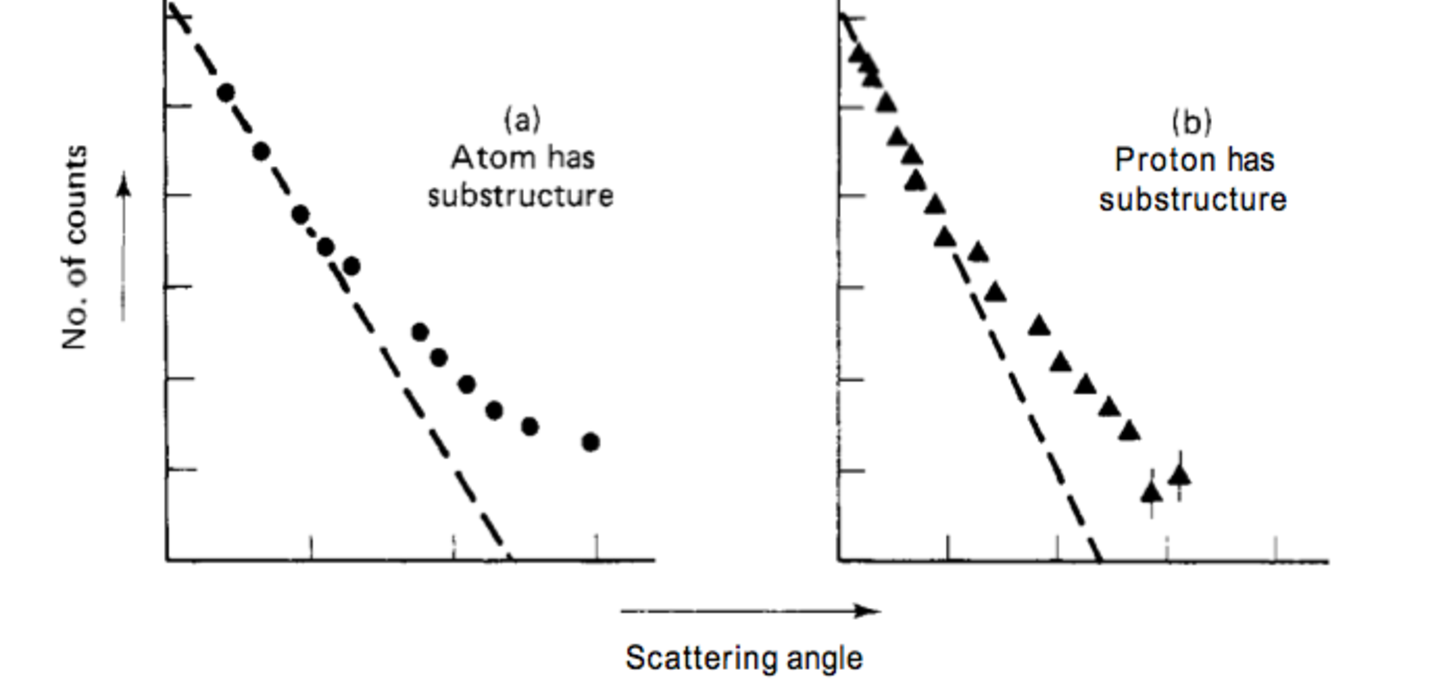
\includegraphics[width = .6\textwidth]{protonSubstructureScattering}
\caption[Scattering at SLAC shows proton substructure]{The dashed line shows expectation if positive charge was uniformly distributed in a) the atom and b) the proton \cite{IEP}.}
\label{fig:protonSubstructureScattering}
\end{center}
\end{figure}





\section{quark model}

In parallel with these developments, experiments detected particles that behaved differently from those currently known. In 1949 a neutral particle, eventually called the $K^0$, was found to decay into a $\pi^+$ and a $\pi^-$. In 1950 another neutral particle was found which decayed into a proton and a negatively charged pion. These newly discovered particles were labeled strange. By 1953 this strange label was found to be a quantum number that had to be conserved just like electric charge, which follows from the fact that these new strange particles are always created in pairs. In 1961 Gell-Mann was able to organize all the known particles using what he called the Eightfold Way. All the known mesons and baryons were arranged in a hexagon based on their electric charge and strangeness.  Gell-Mann went even further by proposing that these meson and baryons were actually composed of smaller particles called quarks. He used these quarks to explain why the mesons and baryons were able to be grouped so nicely. His model consisted of three quarks, the up quark, the down quark, and the strange quark. He also theorized these quarks were bound together by a force mediated by a gluon; a spin 1 boson. The quark makeup of the eight lightest baryons are shown in Table \ref{tab:baryontable}. Today we know that there are six quarks, not just the three that were originally proposed. 

\begin{table}[h!]
\begin{center}
\begin{tabular}{|c|c|c|c|c|c|c|} \hline
particle & quark content & rest mass & isospin & $J^p$ & charge & strangeness \\
\hline
p			& uud & 938.27 MeV/$c^2$ 		& 1/2 & $1/2^+$ & +1 & 0  \\
n			& udd & 939.57 MeV/$c^2$		& 1/2 & $1/2^+$ & 0   & 0  \\
$\Sigma^+$	& uus & 1189.37 MeV/$c^2$		& 1    & $1/2^+$ & +1 & -1 \\
$\Sigma^0$	& uds & 1192.64 MeV/$c^2$		& 1    & $1/2^+$ & 0 & -1 \\
$\Sigma^-$	& dds & 1197.45 MeV/$c^2$		& 1    & $1/2^+$ & -1 & -1 \\
$\Lambda^0$	& uds & 1115.68 MeV/$c^2$		& 0    & $1/2^+$ & 0 & -1 \\
$\Xi^0$		& uss & 1314.86 MeV/$c^2$		& 1/2  & $1/2^+$ & 0 & -2 \\
$\Xi^-$		& dss & 1321.71 MeV/$c^2$		& 1/2  & $1/2^+$ & -1 & -2 \\
\hline
\end{tabular}
\caption{The eight lightest baryons in the quark model}
\label{tab:baryontable}
\end{center}
\end{table}



\section{Electron-Proton Scattering and Structure Functions}

The proton structure can be investigated through the study of electron-proton scattering. The differential cross section for electron-proton deep inelastic scattering, such as the experiments performed at SLAC, can be written in terms of two proton structure functions $W_1(Q^2, x)$ and $W_2(Q^2, x)$.
\begin{equation}
\frac{\text{d}\sigma}{\text{d}\Omega} = \left(\frac{\text{d}\sigma}{\text{d}\Omega}\right)_{mott}\left[2W_1\tan^2\left(\frac{\theta}{2}\right) + W_2\right]
\end{equation}
where $\left(\frac{\text{d}\sigma}{\text{d}\Omega}\right)_{mott}$ is the well-known Mott cross section.

In the deep inelastic scattering limit, where the momentum transfer $Q^2\rightarrow\infty$ and proton momentum $p\rightarrow\infty$, but $x = -\frac{q^2}{2q\cdot p}$ stays fixed, Bjorken predicted the $Q^2$ dependence of the structure functions would disappear. We call this Bjorken scaling.
\begin{eqnarray}
\lim\limits_{Q^2\rightarrow\infty, x \text{ fixed}}& MW_1(Q^2,x) &= F_1(x) \label{eq:bjscaling1}\\
\lim\limits_{Q^2\rightarrow\infty, x \text{ fixed}}& -\frac{q^2}{2Mx}W_2(Q^2,x) &= F_2(x) \label{eq:bjscaling2}
\end{eqnarray}
Although Bjorken scaling cannot hold exactly in any relativistic field theory \cite{AlderTungPhysRevLett.22.978}, experiments have shown approximate Bjorken scaling. The structure functions in equations \ref{eq:bjscaling1} and \ref{eq:bjscaling2} can be written as $F_1(Q^2,x)$ and $F_2(Q^2,x)$ with the dependence on $Q^2$ being logarithmic. This can be seen in Fig. \ref{fig:F2Scaling}. It was found that Bjorken scaling up to logarithmic violations could be explained in asymptotically free field theories \cite{Gross:1992cw}. This led to the asymptotically free theory of Quantum Chromo Dynamics we have today. 
\begin{figure}
\begin{center}
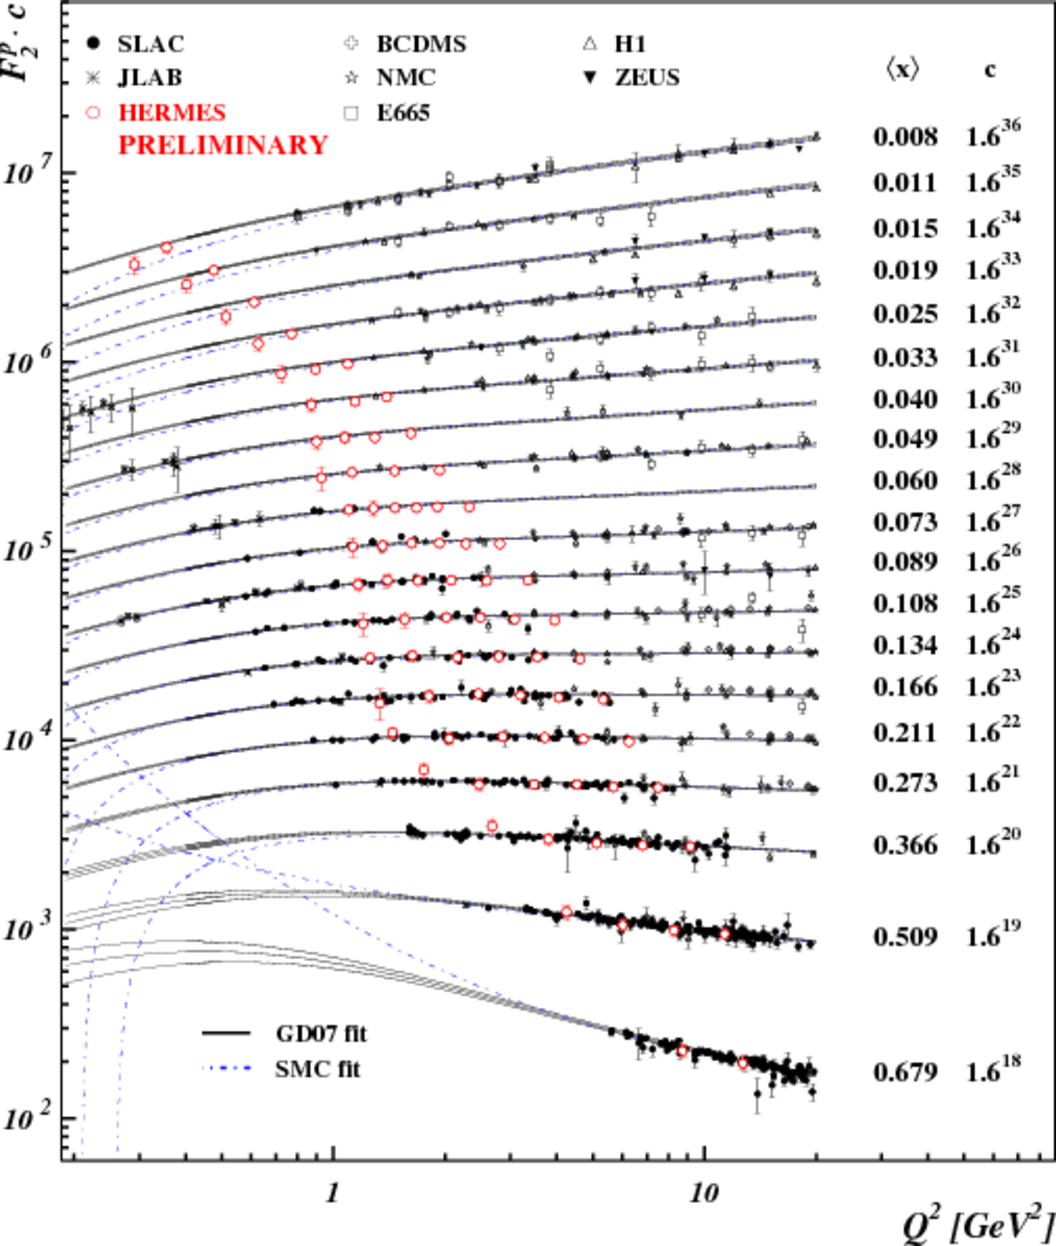
\includegraphics[width = .6\textwidth]{StructFunc2}
\caption[Scaling of the proton structure function $F_2$]{The proton stucture funtion shows approximate Bjorken scaling.}
\label{fig:F2Scaling}
\end{center}
\end{figure}



\section{Factorization theorem and the unpolarized parton distribution function}

The factorization theorem says that in the DIS limit,  scattering occurs between free partons. Because of this, we are able build up the structure functions for the proton from distributions of its constituent partons. 
\begin{eqnarray}
F_1(Q^2,x) &= \sum\limits_a \int\limits_x^1 \frac{\text{d}\xi}{\xi}f_a(\xi,\mu)H_{1a}\left(\frac{x}{\xi},\frac{Q}{\mu}, \alpha_s(\mu)\right) + \text{ remainder}\\
\frac{1}{x}F_2(Q^2,x) &= \sum\limits_a \int\limits_x^1 \frac{\text{d}\xi}{\xi}f_a(\xi,\mu)\frac{\xi}{x}H_{2a}\left(\frac{x}{\xi},\frac{Q}{\mu}, \alpha_s(\mu)\right) + \text{ remainder}
\end{eqnarray} 
Here $f_a(\xi,\mu)$ is the unpolarized parton distribution function of flavor "$a$". It gives the probability of finding a free quark for flavor $a$ inside the proton with momentum fraction $\xi$. The renormalization scale, $\mu$, is free to be chosen. The functions $H_{1a}$ and $H_{2a}$ are the hard scattering coefficients which can be calculated. The convenient choice of $\mu = Q$ will be used.\cite{factorization} At leading order, the form of the structure functions simplify \cite{IEP}.

\begin{equation}
F_2(Q^2,x) = 2x F_1(Q^2,x) = \frac{1}{2}\sum\limits_a e_a ^2 f_a(x, Q)
\end{equation} 
Where $e_a$ is the charge of parton $a$.

The factorization theorem can also be applied directly to the cross sections. In this manner, we can write the cross section of electron-proton scattering directly in terms of parton distribution functions and parton cross sections as seen in Fig.~\ref{fig:FactDIS}.
\begin{equation}
\sigma_{ep} = \sum\limits_a \int\limits_x^1 \text{d}\xi f_a(\xi) \hat{\sigma}_{ea}\left(\frac{x}{\xi},Q^2\right)
\end{equation}
Where $\hat{\sigma}_{ea}$ is a calculable cross section for electron scattering off a parton of type $a$. In this way the factorization theorem can be generalized to other high energy processes.\cite{factorization}
The unpolarized distribution function $f_1(x)$ is well known. It can be extracted by fitting a large number of data points from different DIS experiments at different values of $Q^2$ and $x$ \cite{unpolDisFuncPic}. In Fig.~\ref{fig:f1} the unpolarized distribution functions for different partons are shown. Not surprisingly partons carrying the largest momentum fraction $x$ are the up quark and down quark. 
\begin{figure}[!tbp]
  \centering
  \subfloat[Electron proton scattering]{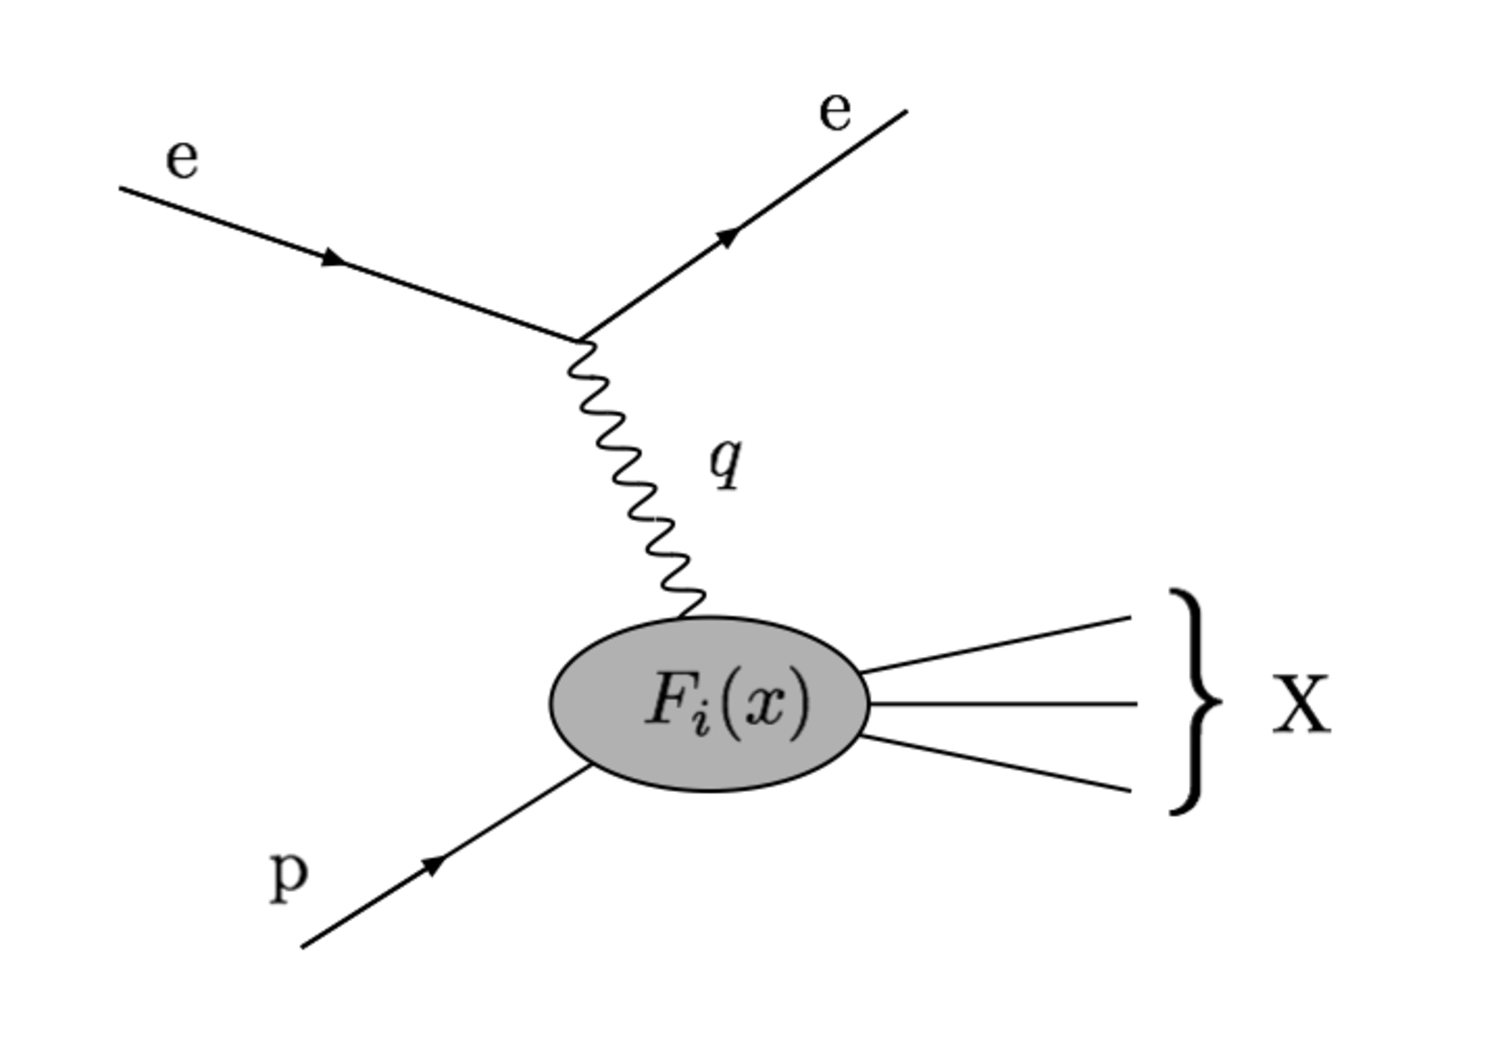
\includegraphics[width=0.55\textwidth]{epScattering}\label{fig:epScat}}
  \hfill
  \subfloat[Scattering becomes electron off quark a in factorization picture]{\includegraphics[width=0.45\textwidth]{factorizationDis}\label{fig:FactDIS}}
  \caption{Factorization theorem of e + p $\rightarrow$ X}
\end{figure}
\begin{figure}
\begin{center}
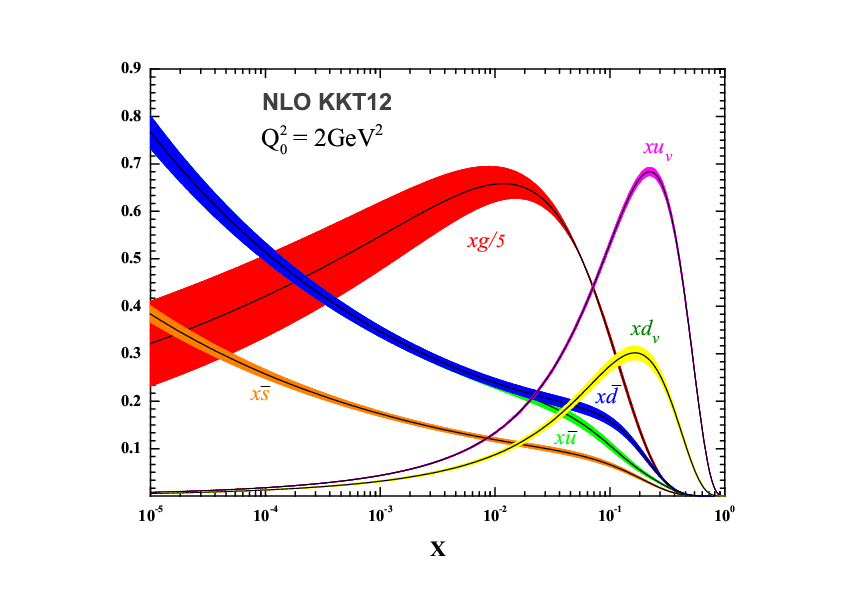
\includegraphics[width = .8\textwidth]{unpolDistFunct}
\caption[unpolarized parton distrubution function]{The unpolarized parton distribution functions as a function of $x$ at initial scale $Q^2_0 = 2 \text{ GeV}^2$ in the NLO approximation \cite{unpolDisFuncPic}.}
\label{fig:f1}
\end{center}
\end{figure}

\FloatBarrier

%\section{Spin-dependent parton distributions}
%
%While the unpolarized distribution tells us some information about the number density of quarks inside a proton, it does not give a complete picture, and does nothing to answer the question about the origin of proton spin. For this we need to look at two other parton distribution functions: the helicity distribution function $g_1(x)$ (sometimes written $\Delta q(x)$), and the transversity distribution function $h_1(x)$ (sometimes written $\Delta_T q(x)$). In the infinite momentum reference frame of the proton with the proton's spin aligned to its direction of motion, the helicity distribution describes the number of quarks with their spin aligned minus the number of quarks with their spin anti-aligned with the proton's spin carrying momentum fraction $x$. Similarly, the transversity distribution function, which wasn't even considered until Ralston and Soper introduced it in 1979\cite{transIntroduced}, describes the number of quarks with their spin aligned minus the number of quarks with their spin anti-aligned with the proton's spin carrying momentum fraction $x$ when the proton's spin in perpendicular to its direction of motion. These parton distribution functions are represented pictorially in figure \ref{fig:PDFs}.  
%\begin{figure}
%\begin{center}
%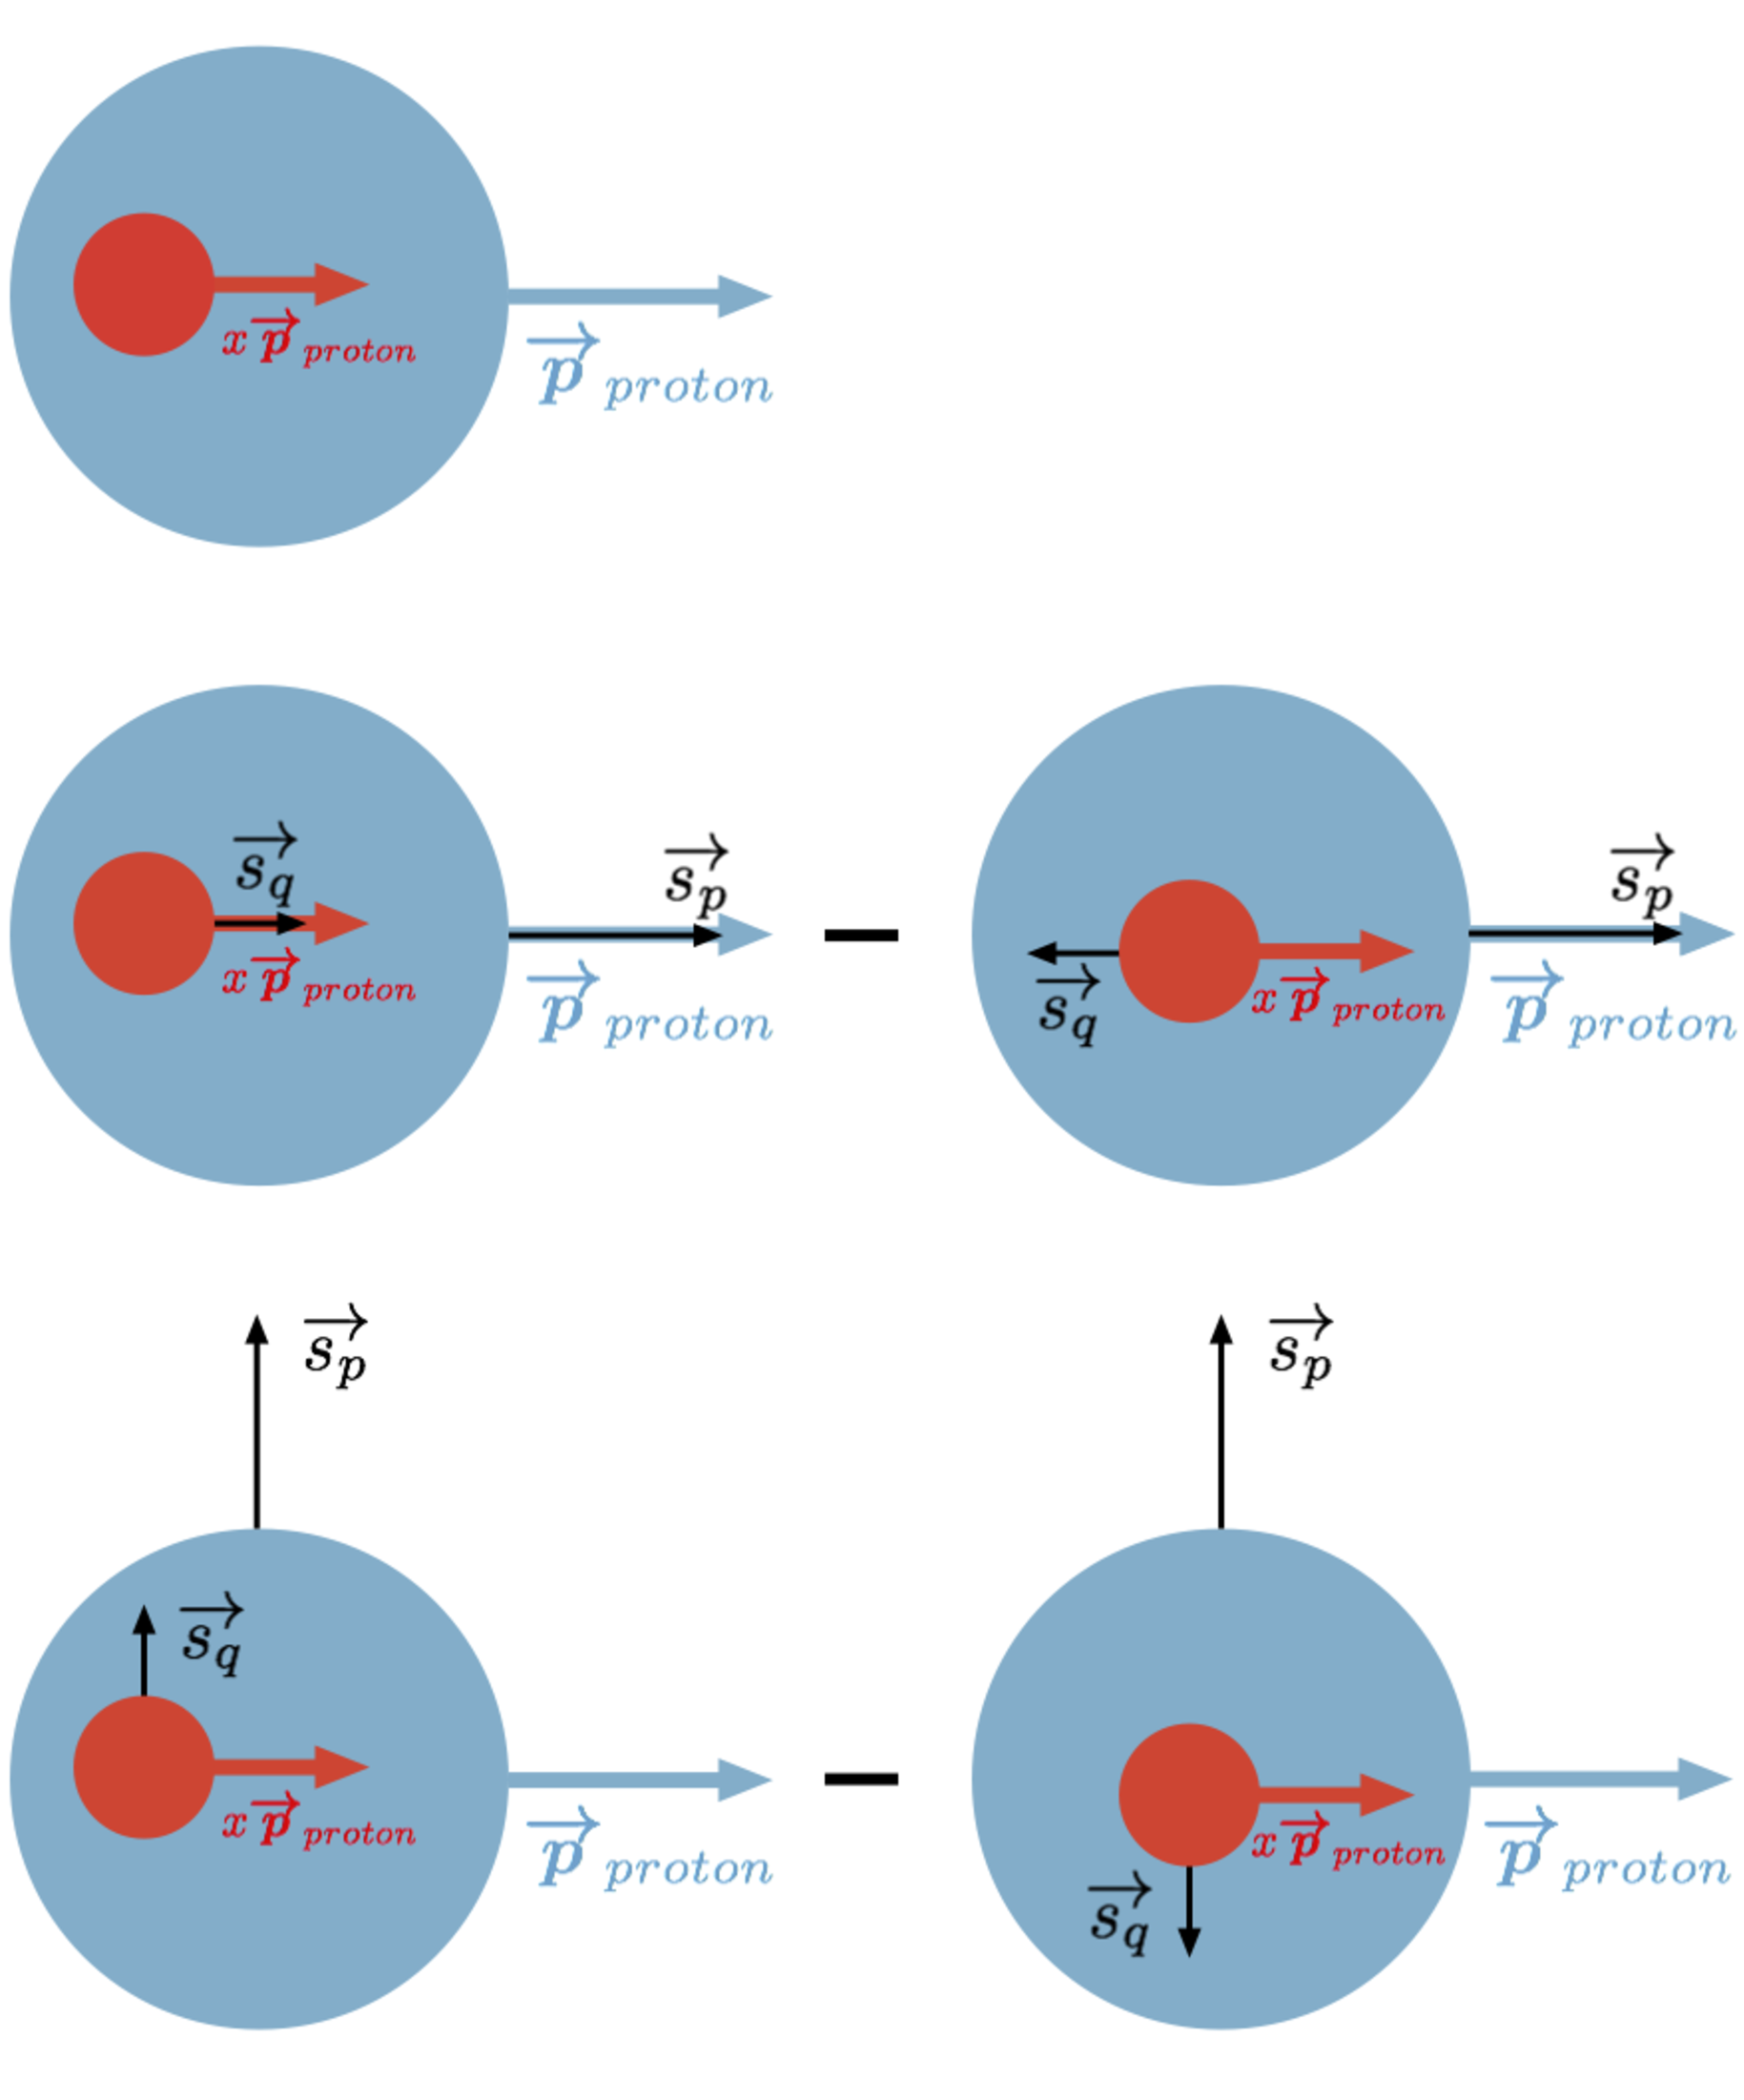
\includegraphics[width = .7\textwidth]{allDistsPic3}
%\caption[Visual representation of unpolarized, hellicity, and transversity distribution functions]{Top: Unpolarized distribution function $f_1(x)$ \\
%Middle: Helicity distribution function $g_1(x)$ \\
%Bottom: Transversity distribution function $h_1(x)$}
%\label{fig:PDFs}
%\end{center}
%\end{figure}

\chapter{Spin Physics}
While the unpolarized distribution tells us some information about the number density of quarks inside a proton, it does not give a complete picture, and does nothing to answer the question about the origin of proton spin. For this we need to look at spin dependent physics, which gives rise to spin dependent parton distribution functions. One of which will be of interest in the remainder of this thesis. 

\section{Logintudinally Polarized Deep Inelastic Scattering}
A good starting point for the study of spin physics is the polarized version of deep inelastic scattering. Specifically we are interested in a longitudinally polarized lepton beam scattering off of a longitudinally polarized proton. Similarly to the unpolarized case, we can describe it in terms of two structure functions $G_1$ and $G_2$. The difference in cross sections when the beam and proton are polarized in the same versus opposite directions is given by
\begin{equation}
\frac{\text{d}^2 \theta^{\substack{\leftarrow \\ \leftarrow}}}{\text{d} \Omega \text{d}E^{'}} - \frac{\text{d}^2\theta^{\substack{\leftarrow \\ \rightarrow}}}{\text{d}\Omega\text{d}E^{'}} = \frac{4\alpha^2E^{'}}{Q^2E}\left[(E+E^{'}cos\theta)MG_1(\nu,Q^2) - Q^2G_2(\nu,Q^2)\right],
\end{equation}
where $E$ and $E^{'}$ are the energies of the lepton in the initial and final states, $\nu = p\cdot q/M$, and $G_1$ and $G_2$ are spin dependent structure functions. In the deep inelastic scattering limit the structure functions $G_1$ and $G_2$ can be written in terms of  dimensionless structure functions that show approximate Bjoken scaling \cite{longReviewPaper}. 
\begin{eqnarray}
\lim\limits_{Q^2\rightarrow\infty, x \text{ fixed}}& M^2G_1(\nu,Q^2) &= g_1(x) \label{eq:g1}\\
\lim\limits_{Q^2\rightarrow\infty, x \text{ fixed}}& M\nu^2G_2(\nu,Q^2) &= g_2(x) \label{eq:g2}
\end{eqnarray}
At leading twist, the contribution from $g_2$ vanishes. The spin dependent structure function $g_1$ can be build up from parton distribution functions in the same way as the unpolarized structure functions. At leading order $g_1$ is given by
\begin{equation}
g_1(x,Q^2) = \frac{1}{2} \sum\limits_a e^2_a\left(\Delta f_a(x,Q^2) + \Delta \bar{f}_a(x,Q^2)\right).
\end{equation}
Called the ``helicity distribution function", $\Delta f$ describes, in the infinite momentum frame of the proton, the number of quarks inside a longitudinally polarized proton with their spin aligned minus the number of quarks with their spin anti-aligned with the proton's spin, carrying momentum fraction $x$ \cite{longReviewPaper}.


In 1997 the HERMES collaboration measured $g_1$ using a combination of inclusive and semi-inclusive lepton-nucleon deep inelastic scattering data \cite{hermesHel}. The data was taken with 27.6 GeV longitudinally polarized positron beam scattering off a longitudinally polarized hydrogen gas target. They constructed a single spin asymmetry $A_{||}$ in the number of scattered positrons. 
\begin{equation}
A_{||} = \frac{N^-L^+ - N^+L^-}{N^-L_P^+ + N^+L_P^-} 
\end{equation}
Where $N^+(N^-)$ is the number of positrons scattered when the target spin is parallel(antiparallel) to the positron beam spin. The luminosities are $L^+$, $L^-$ when the target spin is parallel or antiparallel with the beam spin, while $L^+_P$, $L^-_P$ are weighted luminosities. The structure function $g_1$ was extracted based on its relation to this asymmetry,
\begin{equation}
\frac{g_1}{F_1} = \frac{1}{1+\gamma^2}\left[\frac{A_{||}}{D} + (\gamma - \eta)A_2\right]
\end{equation}
where $\gamma = 2Mx/\sqrt{Q^2}$. Here $A_2$ was previously measured to be small\cite{hermesHel}\cite{strucFuncsg1g2}.
HERMES is not the only collaboration to extract the helicity distribution. The HERMES data, along with other data from other experiments, is shown in figure \ref{fig:helicityDist}. 
 \begin{figure}
\begin{center}
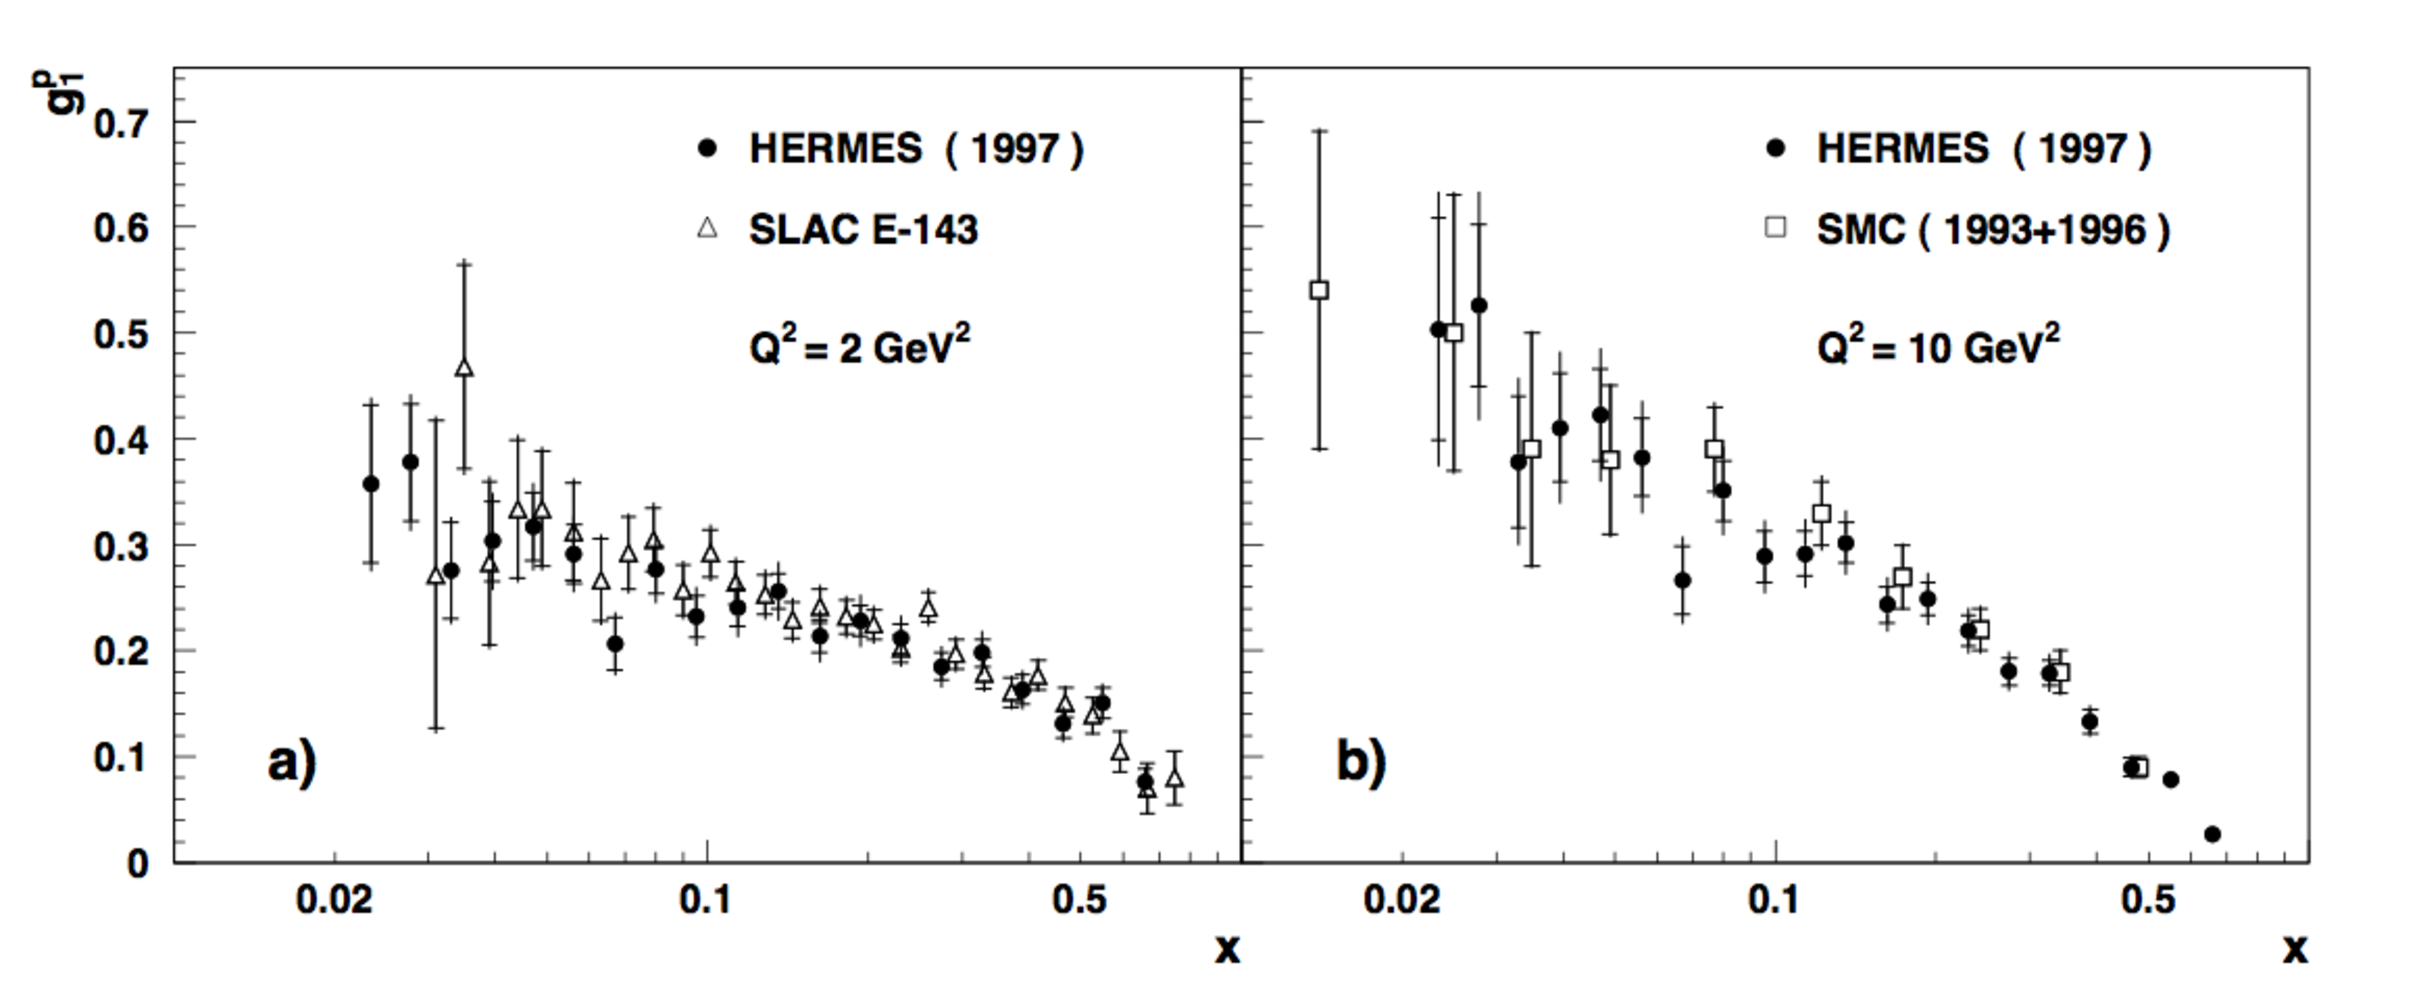
\includegraphics[width = 1\textwidth]{helicityDistFromHermes}
\caption[HERMES results for helicity distribution function]{The helicity distribution as a function of momentum fraction $x$ for $Q^2$ = 2 GeV$^2$ and 10 GeV$^2$.}
\label{fig:helicityDist}
\end{center}
\end{figure}

\section{Proton Spin Crisis}
However the spin of the proton comes about, it must be conceived from the spin of the quarks, $\Sigma$, the orbital angular momentum of the quarks, $L_q$, the orbital angular momentum of the gluons, $L_g$, and the spin of the gluon, $\Delta G$. These must sum to equal the spin of the proton.
\begin{equation}
\frac{1}{2} = \frac{1}{2}\Sigma + L_q + L_g + \Delta G
\end{equation}
In the naive quark model, it was expected that the entirety of the proton spin would be carried by the three valence quarks. In a relativistic theory with QCD corrections, only about 60\% of the proton spin is thought to be carried by the quarks. The initially measured value of $\int\limits_0^1 \text{d}x g_1(x)$, however corresponds to a value of $\Sigma$ of $0.120 \pm 0.16$ or consistent with zero \cite{jaffeWhereSpinComeFrom}. This suggests that virtually none of the proton spin in carried by valence quarks. More recent measurements provide a value of $0.27\pm 0.05$ for $\Sigma$, still much smaller than the theoretical expectation from relativistic models \cite{jaffeWhereSpinComeFrom}.  

It is possible that the contribution to proton spin from gluon spin is larger than previously thought. A global analysis of data from both STAR and PHENIX suggest the contribution from $\Delta G$ is sizable after all \cite{deFlorian:2014yva}. More data is needed to form a more conclusive answer. 

\section{Transversity Distribution Function}
So far only logintudinal spin has been taken into account. Another piece to the proton spin puzzle deals with transverse spin. This can be described by another parton distribution function (written $h_1$ or $\Delta_T f$), which wasn't even considered until Ralston and Soper introduced it in 1979 \cite{transIntroduced}, called the ``transversity distribution function". This distribution function describes the number of quarks with their spin aligned minus the number of quarks with their spin anti-aligned with the proton's spin carrying momentum fraction $x$ when the proton's spin is perpendicular to its direction of motion. One might think this is equivalent to the helicity distribution function as the probability of finding a parton whose spin is aligned versus anti-aligned with the proton spin shouldn't depend on the direction of the proton spin. This is true for a proton in its rest frame. However this interpretation of the helicity and transversity distributions are only viable in the infinite momentum frame of the proton. In a relativistic setting such as this, Lorentz boosts cause these distributions to differ \cite{BacchettaThesis}.

Unlike the helicity distribution function, the transversity distribution function does not appear in lepton inclusive deep inelastic scattering due to its chiral-odd nature. In order to observe its effects, it must be paired with another chiral-odd object to create a chiral-even observable, making it harder to access. Because of this, the transversity distribution function is currently not very well-known.
\section{First Experimental Measurements of Transversity}
\subsection{In Single Hadron Production semi-inclusive DIS}
The detection of a single hadron in the final state introduces another chiral-odd piece to the cross section in the form of a quark fragmentation function which describes how probable it is for a quark to fragment into a given hadron. When paired with the transversity distribution, a chiral-even observable is created, allowing the transversity distribution to be probed. This was first done by HERMES through semi-inclusive DIS of positrons off of a polarized proton target with a single hadron detected in the final state \cite{Airapetian:2004tw, Anselmino:2007fs}, 
\begin{equation}
e+p^\uparrow \rightarrow e + h + X.
\end{equation}
Just as in the experiment to measure the helicity distribution, a single spin asymmetry was detected \cite{Airapetian:2004tw},
\begin{equation}
A^h_{UT}(\phi,\phi_S) = \frac{1}{|S_T|}\frac{N^\uparrow_h(\phi,\phi_S) - N^\downarrow_h(\phi,\phi_S)}{N^\uparrow_h(\phi,\phi_S) + N^\downarrow_h(\phi,\phi_S)}
\end{equation} 
where $N^{\uparrow(\downarrow)}_h(\phi,\phi_S)$ is the number of hadrons produced at azimuthal angle $\phi$ and angle $\phi_S$ to the proton spin when the spin is polarized up(down), and $|S_T|$ is the polarization of the target proton spin. 

There are two sources of this asymmetry present in the cross section. These are the Collins azimuthal moment $\langle\sin(\phi+\phi_S)\rangle_{UT}^h$ and the Sivers moment $\langle\sin(\phi-\phi_S)\rangle_{UT}^h$. These were both measured and can be seen in figures \ref{fig:singleHadHERMES}a, \ref{fig:singleHadHERMES}b. From these transversity could be extracted \cite{Anselmino:2007fs}.

\begin{figure}
	\caption{Single Spin Asymmetry in SIDIS single hadron production measurements from HERMES \cite{Airapetian:2004tw}}
	\label{fig:singleHadHERMES}
	\begin{tabular}{cc}
	\subfloat[Measurement of Collins moment]{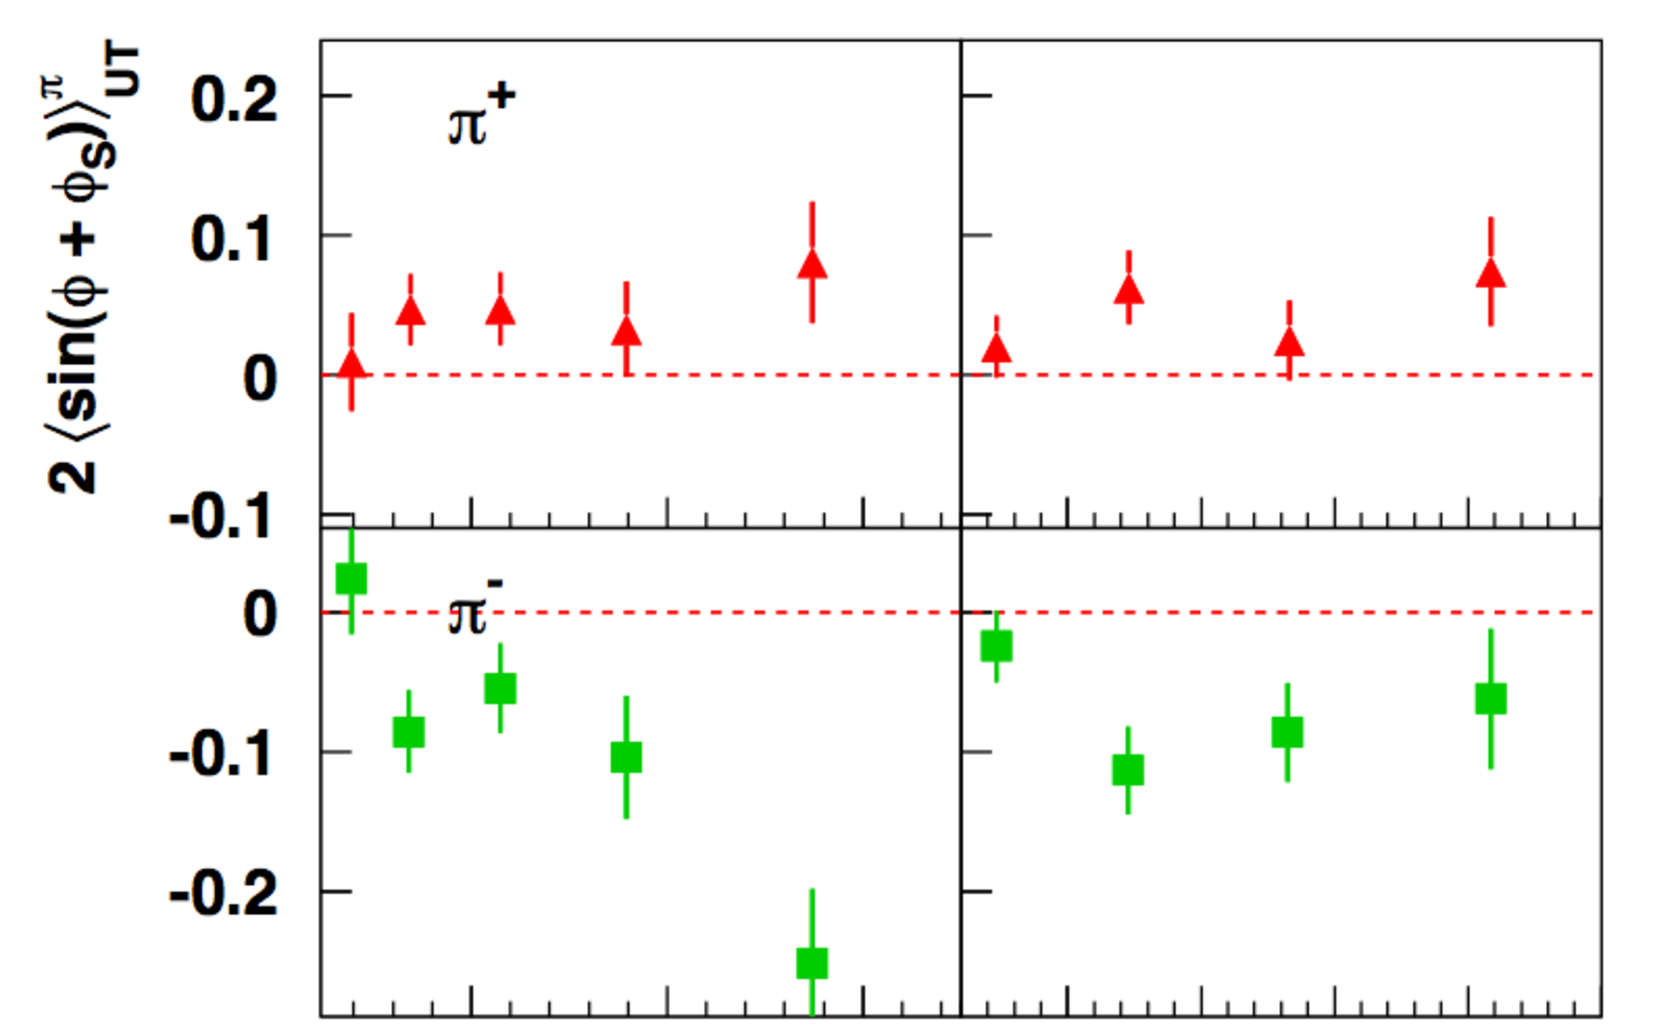
\includegraphics[width=.5\textwidth]{colinsMomentSHsidis}\label{fig:colMoment}} & \subfloat[Measurement of Sivers moment]{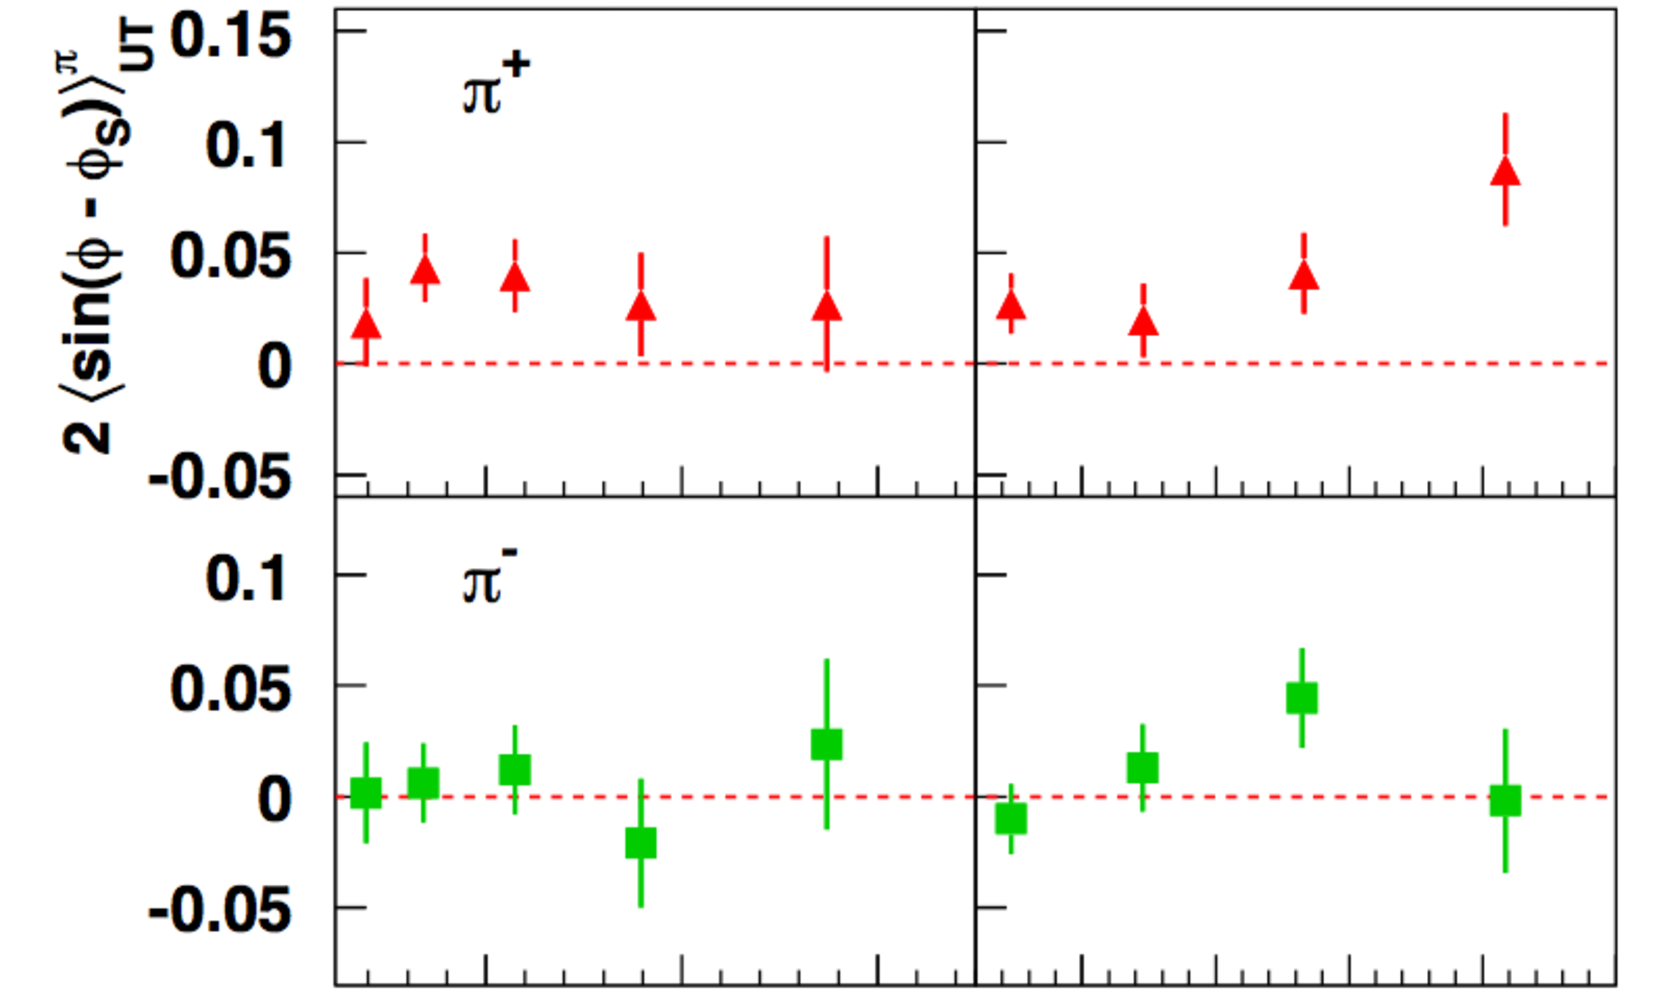
\includegraphics[width=.5\textwidth]{siversMomentSHsidis}\label{fig:sivMoment}} 
	\end{tabular}
\end{figure}
\FloatBarrier
\subsection{In Double Hadron Production semi-inclusive DIS}
\label{subSec:doublehadProd}
Quark fragmentation into two hadrons in the same jet, as described by the interference fragmentation function (IFF) and shown in Fig.~\ref{fig:IFF}, can also be paired with transversity to create a chiral-even observable \cite{EFREMOV1992394, Bianconi:1999cd}. This was done by the COMPASS collaboration \cite{compassRes} and the HERMES collaboration \cite{hermesRes} $via$ the process
\begin{figure}
\begin{center}
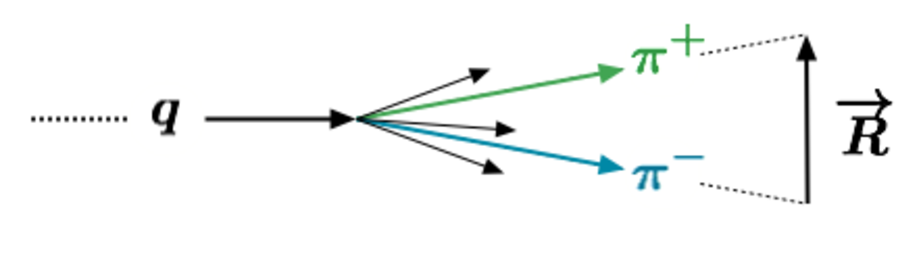
\includegraphics[width = .7\textwidth]{IFFwrite}
\caption[Interference Fragmentation Function]{an outgoing quark fragments into a $\pi^+\pi^-$ pair. This is described by the Interference Fragmentation Function (IFF). The Vector $\vec{R}$ gives the orientation of the pair.}
\label{fig:IFF}
\end{center}
\end{figure}
 \begin{equation}
e+p^\uparrow \rightarrow e + (\pi^+,\pi^-)_{jet} + X.
\end{equation}
Once again a singe spin asymmetry was measured. This is shown in figure \ref{fig:hermesAsym} for HERMES data.
 \begin{figure}
\begin{center}
\includegraphics[width = 1\textwidth]{hermesAsym}
\caption[Single Spin Asymmetry measured by the HERMES collaboration]{Single Spin Asymmetry measured by the HERMES collaboration \cite{hermesRes}}
\label{fig:hermesAsym}
\end{center}
\end{figure}
This asymmetry is related to the transversity distribution by \cite{hermesRes},
 \begin{equation}
A_{UT}^{\sin(\phi_{R\perp}+\phi_S)\sin\theta} = - \frac{1-y}{1-y-\frac{y^2}{2}}\frac{1}{2}\sqrt{1-4\frac{M_\pi^2}{M_{\pi\pi}^2}}\frac{\sum\limits_q e_q^2h_1^q(x)H_{1,q}^{\sphericalangle,sp}(z,M_{\pi\pi})}{\sum\limits_q e_q^2f_1^q(x)D_{1,q}(z,M_{\pi\pi})}
\end{equation}
where $y = (P\cdot q)/(P\cdot k)$, $q$ and $k$ are the momenta of the virtual photon and incoming positron respectively, $H_{1,q}^{\sphericalangle,sp}(z,M_{\pi\pi})$ is the IFF describing the probability of transversely polarized quark q fragmenting into a pion pair with invariant mass $M_{\pi\pi}$ retaining momentum fraction $z$ of the fragmenting quark, and $D_{1,q}(z,M_{\pi\pi})$ is the unpolarized partner of the IFF, $h_1^q(x)$ is the transversity distribution for parton $q$ while $f_1^q(x)$ is the unpolarized parton distribution for parton $q$.

The asymmetry observed in this dihadron production does not depend on parton transverse momentum allowing it to be analyzed in the collinear framework. The single hadron production must be analyzed in the Transverse Momentum Dependent (TMD) framework. TMD factorization has been shown to depend on physical processes; however, collinear factorization is the same from process to process. This makes the asymmetry in dihadron production a useful observable when comparing results in lepton scattering and hadronic collisions as well as when making predictions \cite{univTrans}.  
  
%Go into benefits of the two-hadron process (collinear vs TMD = universal so I can make predictions of hadron processes)

\subsection{Transversity measurment in $p+p$ Collisions}
There are several benefits in measuring the transversity distribution in proton-proton collisions as well. First of all, it can test the universality of the parton distributions. Furthermore, in proton-proton collisions, the momentum fraction carried by the interacting quarks is much higher than the fixed target SIDIS experiments previously discussed. This allows us to extend our knowledge we have of the transversity distribution into a new kinematic regime. 

There are several ongoing measurements at STAR which are sensitive to the transversity distribution, and will thus test the consistency of the extracted transversity. One such experiment uses a single charged hadron, typically a pion, production $p^\uparrow + p \rightarrow \pi + X$ at mid-rapidity coupled to the Collins Fragmentation Function. Another is mid-rapidity W and Z boson production coupled to the Sivers Function. At forward rapidity, neutral pion production is sensitive to the transversity distribution through the Collins function. 
%both the Collins and the Sivers Functions. 

The rest of this thesis will cover the measurement of transversity through double charged hadron production $p^\uparrow + p \rightarrow h_1^+h_2^- + X$ at mid-rapidity. As mentioned in chapter \ref{subSec:doublehadProd}, this is coupled with the Interference Fragmentation Function. Therefore in order to obtain useful information about the transversity distribution, we need a measurement of the IFF. 

%\section{Use or not?}
%We know a lot about the internal structure of the proton. We have known for a quite a while that the proton is made up of even smaller particles. In 1968 deep inelastic scattering experiments at the Stanford Linear Accelerator (SLAC) showed the first evidence the proton was made up of quarks, and in 1979 the Positron-Electron Tandem Ring Accelerator (PETRA) produced evidence of gluons inside the proton. We know that the intrinsic angular momentum (or spin) of the proton is $\frac{1}{2}$.  
%however, we are not quite sure why. 
Since the proton is made up of quarks and gluons, it seems like the spin of the proton needs to come from these constituents, so we look at the parton kinematics inside the proton. This is described to leading order by a set of three distributions -  the unpolarized distribution $f_1(x)$, the helicity distribution function $g_1(x)$, and the transversity distribution function $h_1(x)$.            
%
%The unpolarized distribution function describes the probability of finding a parton with momentum fraction $x$ inside of the proton. This is known quite well from deep inelastic scattering (DIS). The helicity distribution function is similar. It also describes the probability to find a parton with momentum fraction $x$ inside the proton but with a difference. The proton in this case has its spin direction aligned with its momentum, and the probability is the difference in finding the quark's spin aligned vs anti-aligned with the proton's spin. Like the unpolarized distribution, this too is known quite well from DIS experiments.
%
%
%We know a lot about the structure of the proton. Thanks to something we know it consists of partons (quarks and gluons). We know that the valence quarks are uud. other stuff. We know it's intrinsic angular momentum (or spin) is $\frac{1}{2}$. However we still don't know why it's spin is always $\frac{1}{2}$.  The naive explanation is that it comes directly from the spin of the two up quarks and the down quark that make up the proton. However this does not totally account for the proton's spin. The spin of gluons and the orbital angular momentum of both the quarks and gluons needs to be taken into account.   
%
%
%\section{use or not 2?}
%
%In order to understand the spin of the proton, we need to look to the patron distribution functions. This set of three functions tell the complete story of parton kinematics inside the proton at leading order. The first parton distribution function called the unpolarized distribution function $f_1(x)$ is well known from deep inelastic scattering (DIS). It tells the probability of finding a parton with momentum fraction $x$ inside of the proton. That is, if the proton has a momentum $\vec{P}$, $f_1(x)$ tells the probability of finding a parton with momentum $x\vec{P}$.  The second parton distribution function is also fairly well known from DIS. It is called the helicity distribution function and denoted $g_1(x)$. This distribution function tells the difference in probability of finding a parton whose spin is aligned with the proton's spin with momentum fraction $x$ and of finding a parton whose spin is anti aligned with the proton spin with momentum fraction $x$ inside a proton whose spin is aligned with its direction of motion. The final parton distribution function, which wasn't even considered until Ralston and Soper introduced it in 1979\cite{transIntroduced}, is the transversity Distribution function $h_1(x)$. This is very similar to the helicity distribution function. The only difference being the proton spin is perpendicular to the direction of motion for the transversity distribution function instead of aligned with it. These parton distribution functions are represented pictorially in figure \ref{fig:PDFs}. \\
%
%The unpolarized and helicity distributions, which can be seen in figure \ref{pdfDist}, are known accurately for different Bjorken $x$ and momentum transfer of the hard scattering process $Q^2$. On the other hand, the transversity distribution, which can also be seen in figure \ref{pdfDist}, is not well known at all even for just $x$. This is because the transversity distribution function is chiral odd while the unpolarized and helicity distributions are chiral even. This allows the unpolarized and helicity distribution to be accessed through DIS. Since all observables must be chiral even, the transveristy distribution can not be accessed through DIS. It has to be paired with another chiral odd quantity to make a chiral even observable. <??DO I DO SOMETHING HERE SHOWING THAT IT'S CHIRAL ODD WITH SOME PICTURES AND STUFF???> \\ 
%
%\begin{figure}
%\begin{center}
%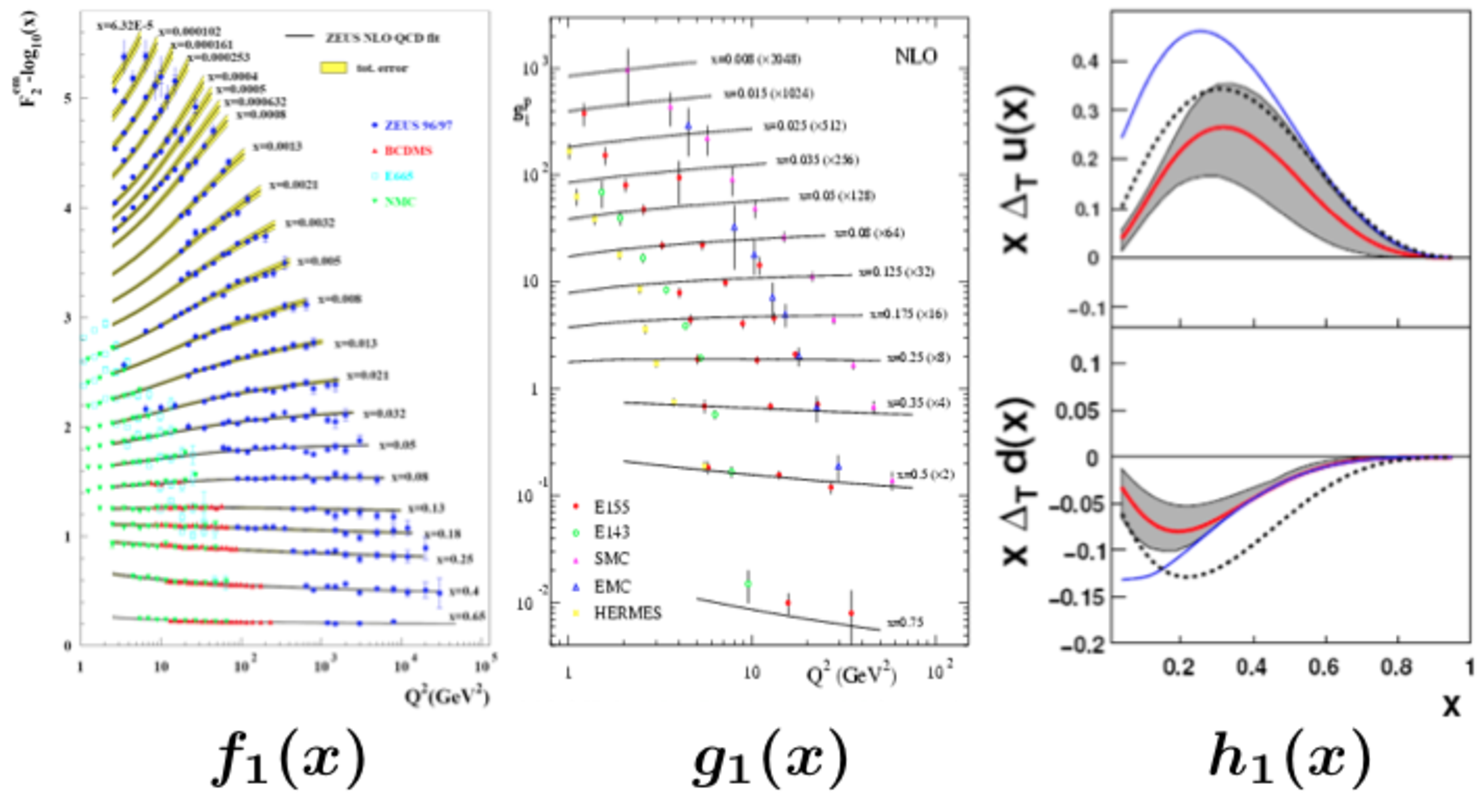
\includegraphics[width = 1\textwidth]{pdfDistributions}
%\caption[Current knowlege of parton distribution functions]{Left and center pannels show the unpolarized and helicity distribution functions as a function of momentum transfer $Q^2$ for different values of the momentum fraction $x$. The right pannel shows out best knowlege of the transversity distribution function for the up quark (top) and the down quark (bottom) vs momentum fraction $x$. The grey band shows the uncertainty of the transversity distribution function. The Blue line is a more leanient uncertainty. The dotted line shows the helicity distribution function for the up and down quarks. <ADD REFERENCES TO THE PLOTS>}
%\label{fig:pdfDist}
%\end{center}
%\end{figure}
%
%Several chiral odd candidates to pair with the transversity distribution function have been considered. One such candidate is a transversely polarized Drell-Yan process. This is not ideal because the cross section is small and involves an antiquark transversity distribution as well. <STUFF ABOUT OTHER POSSIBLE CANDIDATES> The candidates which makes the most sense are chiral odd quark fragmentation functions. 

%\section{Quark Fragmentation and Interference Fragmentation Function get rid of this}
%Due to confinement of quarks, free quarks are never observed. Instead a ``free" quark will pull other partons from the vacuum to form a hadron. This process is called quark fragmentation. We describe this process by fragmentation functions. A fragmentation fucntion $D_{c/C}(z)$ will give the probability of quark $c$ fragmenting into hadron $C$ retaining a fraction $z$ of the fragmenting quark's momentum.
%
%Once again, we can use the factorization theorem to write cross sections in terms of a convolution of partonic pieces. Take a SIDIS of a lepton beam off of a proton where a hadron C is detected.
%\begin{equation}
%\ell + p \rightarrow \ell + C + X
%\end{equation}
%The cross section for this process can schematically be written as 
%\begin{equation}
%\sigma = \sum\limits_{a,c}f_a(x) \otimes \sigma^{\ell a\rightarrow\ell c} \otimes D_{c/C}.
%\end{equation}
%
%\begin{figure}
%\begin{center}
%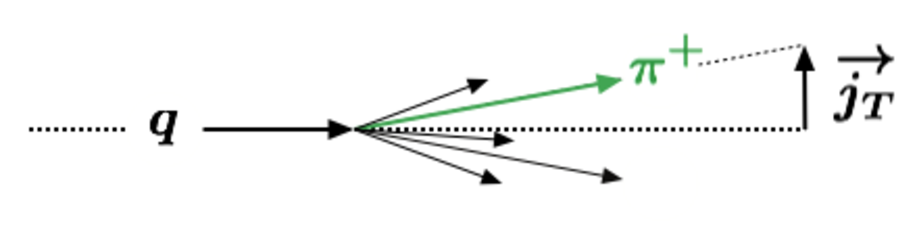
\includegraphics[width = .7\textwidth]{otherFrac2}
%\caption[Collins Fragmentation Function]{an outgoing quark fragments into a $\pi^+$ (or $\pi^-$). This is described by the collins fragmentation function. $\vec{j}_T$ is the component of the pion momentum transvers to the jet axis.} 
%\label{fig:collins}
%\end{center}
%\end{figure}
%
%
%A specific fragmentation function we are interested in is the Interference Fragmentation Function (IFF). The IFF describes the fragmentation of a transversely polarized quark into a pair of oppositely charged pions (figure \ref{fig:IFF}). This can be used to access transversity\cite{accessTransWithIFF}.   
%
%\begin{figure}
%\begin{center}
%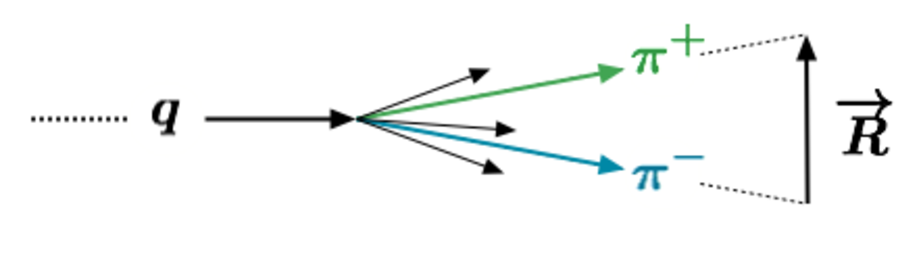
\includegraphics[width = .7\textwidth]{IFFwrite}
%\caption[Interference Fragmentation Function]{an outgoing quark fragments into a $\pi^+\pi^-$ pair. This is described by the Interference Fragmentation Function (IFF). The Vector $\vec{R}$ gives the orientation of the pair.}
%\label{fig:IFF}
%\end{center}
%\end{figure}

\section{Measuring the Interference Fragmentation Function at BELLE}

In our experiment, transversity only shows up as a convolution with the interference fragmentation function, $h_1H_1^\sphericalangle$. In order to isolate transversity in our data we need to know how the interference fragmentation function behaves. The BELLE experiment at KEK has already done this work\cite{belleIFF}. They performed an electron-positron annihilation experiment detecting back-to-back $\pi^+\pi^-$ pairs. The relative angle between the two pions was determined and the modulation, $a_{12}$, of the number of back-to-back pairs found at different values of the relative angle was measured. This modulation, called the Artuo-Collins asymmetry, is related to two IFFs. 
     
\begin{multline}
%\begin{equation}
a_{12} \propto \frac{1}{2} \frac{\sin^2\theta}{1+\cos^2\theta} \left[ \sum_{q,\bar{q}}e_q^2z_1^2z_2^2H_1^{\sphericalangle q}(z_1, m_1^2)H_1^{\sphericalangle \bar{q}}(z_2, m_2^2)\right] \\ \times \left[ \sum_{q,\bar{q}}e_q^2z_1^2z_2^2D^{q}(z_1, m_1^2)D^{\bar{q}}(z_2, m_2^2)\right]^{-1}
%\end{equation}
\label{eq:A-Casym}
\end{multline}

Here $\theta$ is the polar angle defined between the beam axis and the reference axis, $D^q$ is the unpolarized equivalent of the IFF, $z_{1(2)}$ is the energy fraction pion pair 1(2) has, and $m_{1(2)}$ is the invariant mass of pair 1(2). BELLE reported the modulation $a_{12}$ for different $z_1,z_2$ bins as well as different $m_1,m_2$ bins for different quark flavors \cite{belleIFF}. The modulation $a_{12}$ is shown in Fig.~\ref{fig:BelleMod} plotted versus the invariant mass. With this data, Courtoy $et~al$ \cite{extractIFF} were able to extract the Interference Fragmentation Function.

 \begin{figure}
\begin{center}
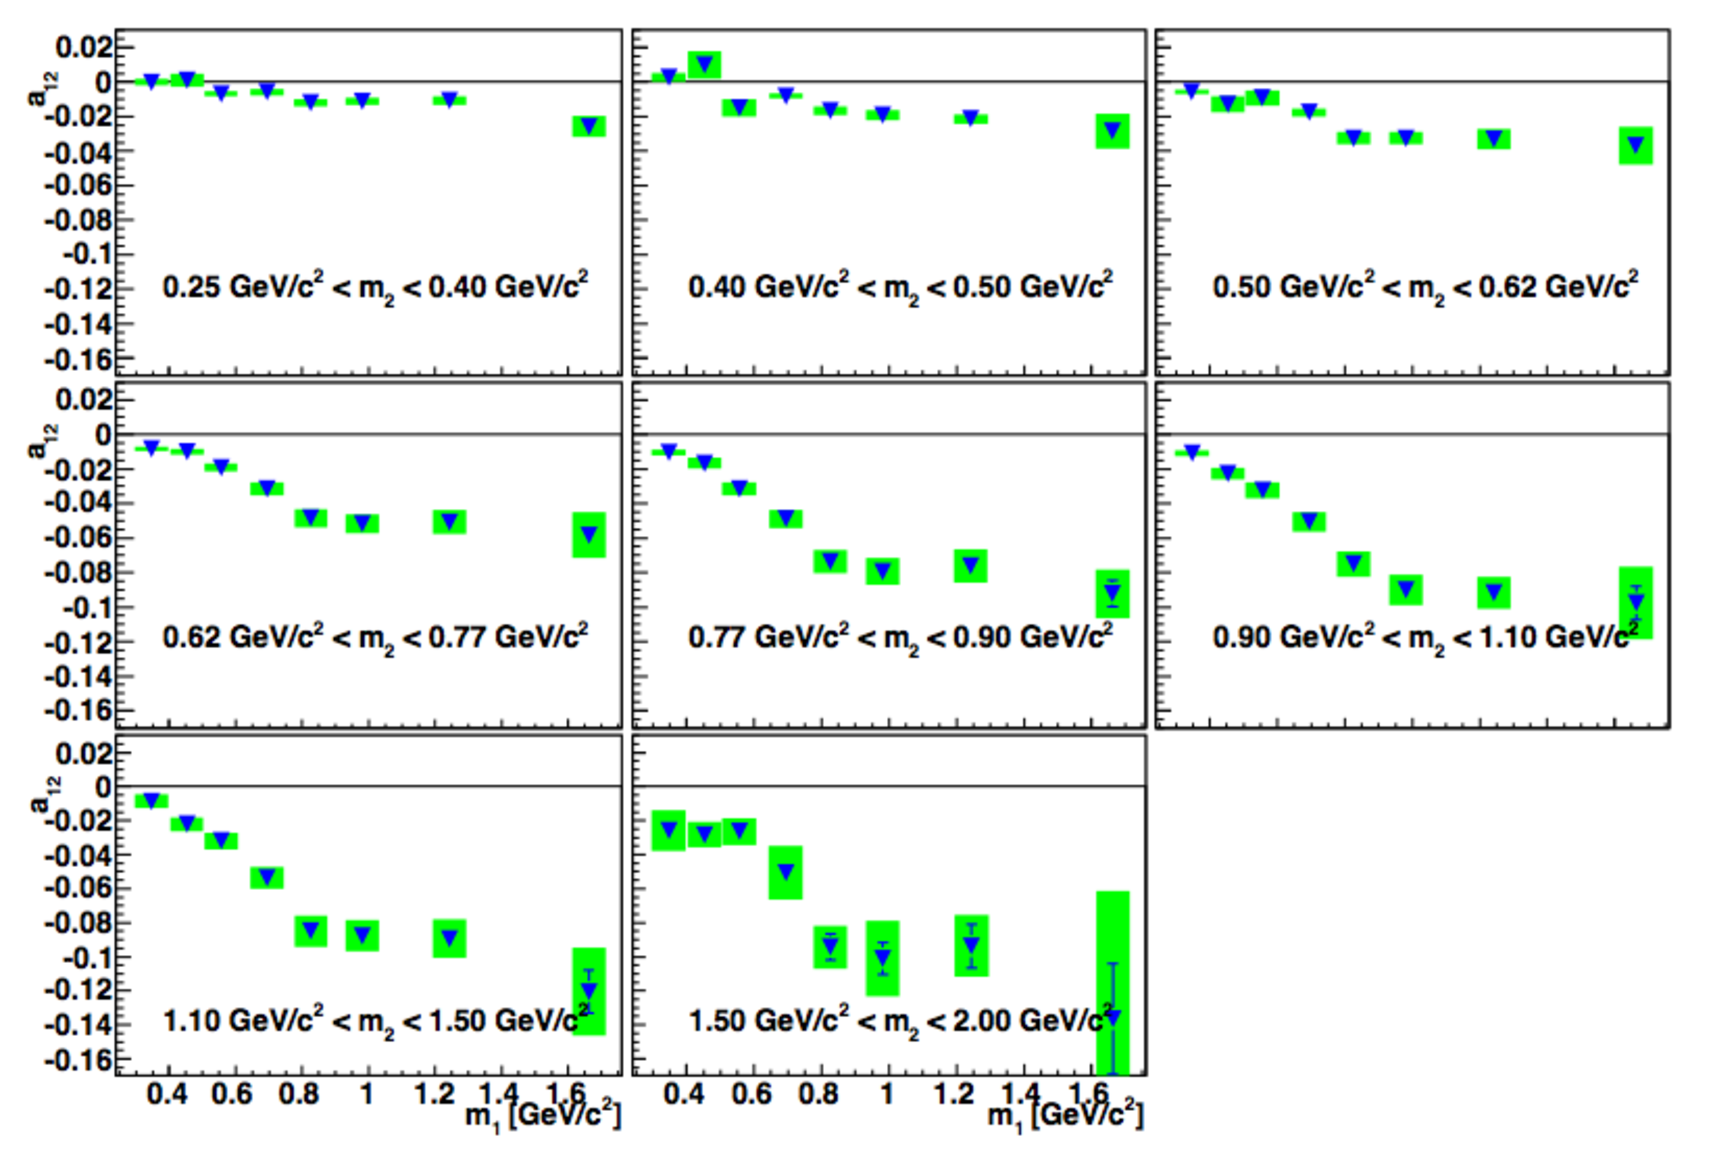
\includegraphics[width = .7\textwidth]{BelleAnnModulationM}
\caption[Asymmetry seen in $e^-e^+$ annihilation at BELLE]{Asymmetry in the number of back-to-back pion pairs seen at BELLE plotted $vs$ the invariant mass \cite{belleIFF}.}
\label{fig:BelleMod}
\end{center}
\end{figure}




%\chapter{Experimental Landscape}
%
%Before getting into my analysis, I would like to start by acknowledging the experiments that have impacted our knowledge of the parton distribution functions. 
%
%\section{Unpolarized Distribution Function}
%
%\section{The Helicity Distribution Funtion}
%
%The helicity distribution $g_1(x)$ has been measured accurately by multiple collaborations. In 1997 the HERMES collaboration measured the helicity distribution using a combination of inclusive and semi-inclusive lepton-nucleon deep inelastic scattering data. \ref{bib:} The data was taken with 27.6 GeV longitudinally polarized positron beam scattering off a longitudinally polarized hydrogen gas target. They constructed an asymmetry $A_{||}$ in the number of scattered positrons. 
%
%\begin{equation}
%A_{||} = \frac{N^-L^+ - N^+L^-}{N^-L_P^+ + N^+L_P^-} 
%\end{equation}
%
%Where $N^+(N^-)$ is the number of positrons scattered when the target spin is parallel(antiparallel) to the positron beam spin. The luminosities are $L^+$, $L^-$ when the target spin is parallel or antiparallel with the beam spin, while $L^+_P$, $L^-_P$ are weighted luminosities. The helicity distribution function was extracted based on its relation to this asymmetry.
%
%\begin{equation}
%\frac{g_1}{F_1} = \frac{1}{1+\gamma^2}\left[\frac{A_{||}}{D} + (\gamma - \eta)A_2\right]
%\end{equation}
%
%   
%Hermes is not the only collaboration to extract the helicity distribution. The Hermes data along with other experiments data is shown in figure \ref{fig:helicityDist}. 
%
%
% \begin{figure}
%\begin{center}
%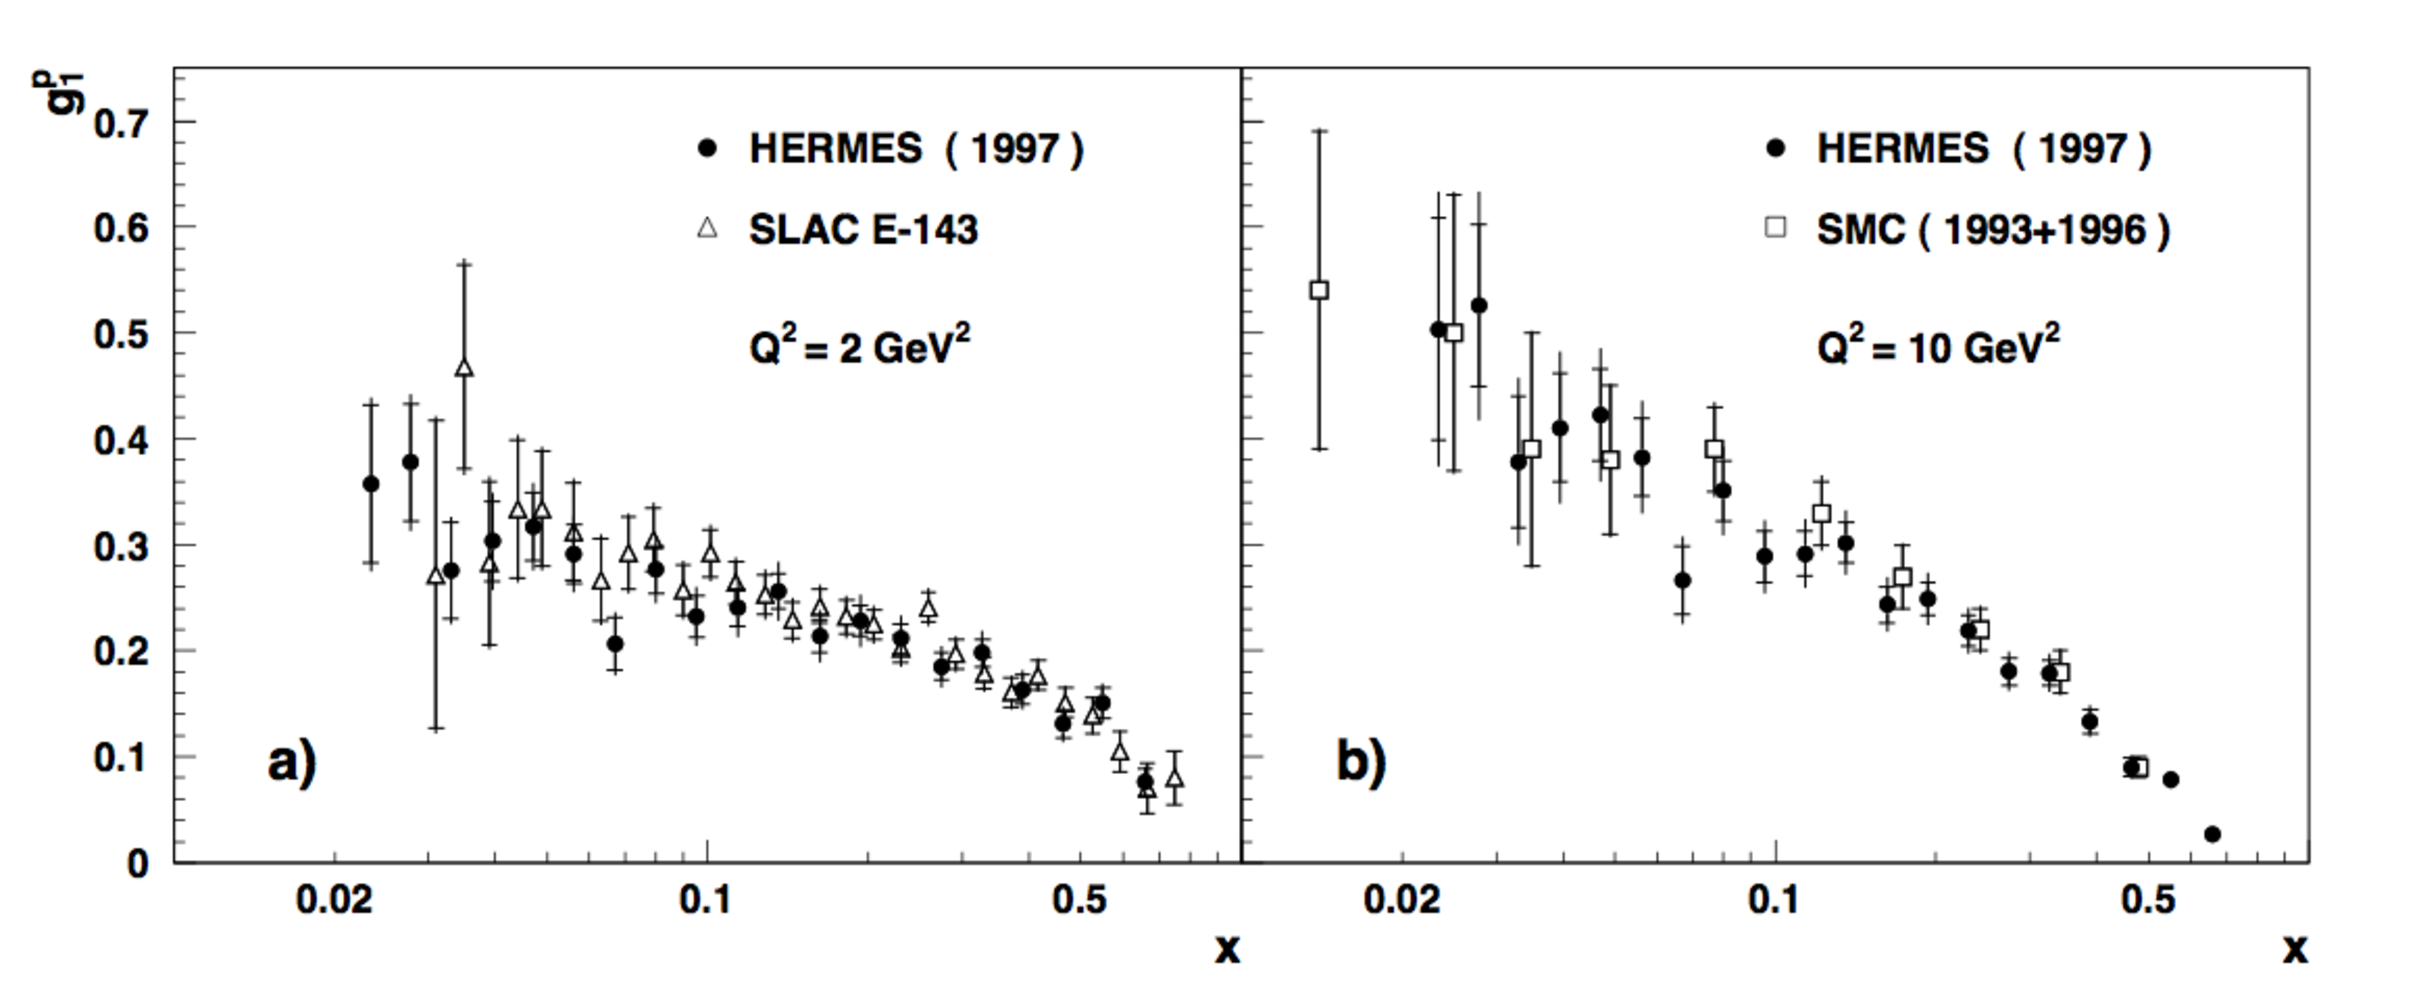
\includegraphics[width = 1\textwidth]{helicityDistFromHermes}
%\caption[HERMES results for helicity distribution function]{The helicity distribution as a functuon of momentum fraction x for $Q^2$ = 2 GeV$^2$ and 10 GeV$^2$.}
%\label{fig:helicityDist}
%\end{center}
%\end{figure}
%
%\FloatBarrier
%\section{Measuring the Interference Fragmentation Function at Belle}
%
%In our experiment, transversity only shows up as a convolution with the interference fragmentation function $h_1H_1^\sphericalangle$. In order to isolate transversity in our data we need to know how the interference fragmentation function behaves. Luckily for us Belle already did this work. They performed an electron positron annihilation experiment detecting back to back $\pi^+\pi^-$ pairs. A relative angle between the two pions was measured and a modulation $a_{12}$ of the number of back to back pairs found at different values of the relative angle was seen. This modulation is related to two IFFs. 
%     
%\begin{multline}
%\begin{equation}
%a_{12} \propto \frac{1}{2} \frac{\sin^2\theta}{1+\cos^2\theta} \left[ \sum_{q,\bar{q}}e_q^2z_1^2z_2^2H_1^{\sphericalangle q}(z_1, m_1^2)H_1^{\sphericalangle \bar{q}}(z_2, m_2^2)\right] \\ \times \left[ \sum_{q,\bar{q}}e_q^2z_1^2z_2^2D^{q}(z_1, m_1^2)D^{\bar{q}}(z_2, m_2^2)\right]^{-1}
%\end{equation}
%\end{multline}
%
%Here $\theta$ is the polar angle defined between the beam axis and the reference axis, $D^q$ is the unpolarized equivalent of the IFF, $z_{1(2)}$ is the energy fraction pion pair 1(2) has, and $m_{1(2)}$ is the invariant mass of pair 1(2). The people at Belle reported the modulation $a_{12}$ for different $z_1,z_2$ bins as well as different $m_1,m_2$ bins for different quark flavors. The modulation $a_{12}$ is shown in figure \ref{fig:BelleMod} plotted versus the invariant mass. With this data, Courtoy et al were able to extract the Interference Fragmentation Function.\cite{extractIFF}
%
% \begin{figure}
%\begin{center}
%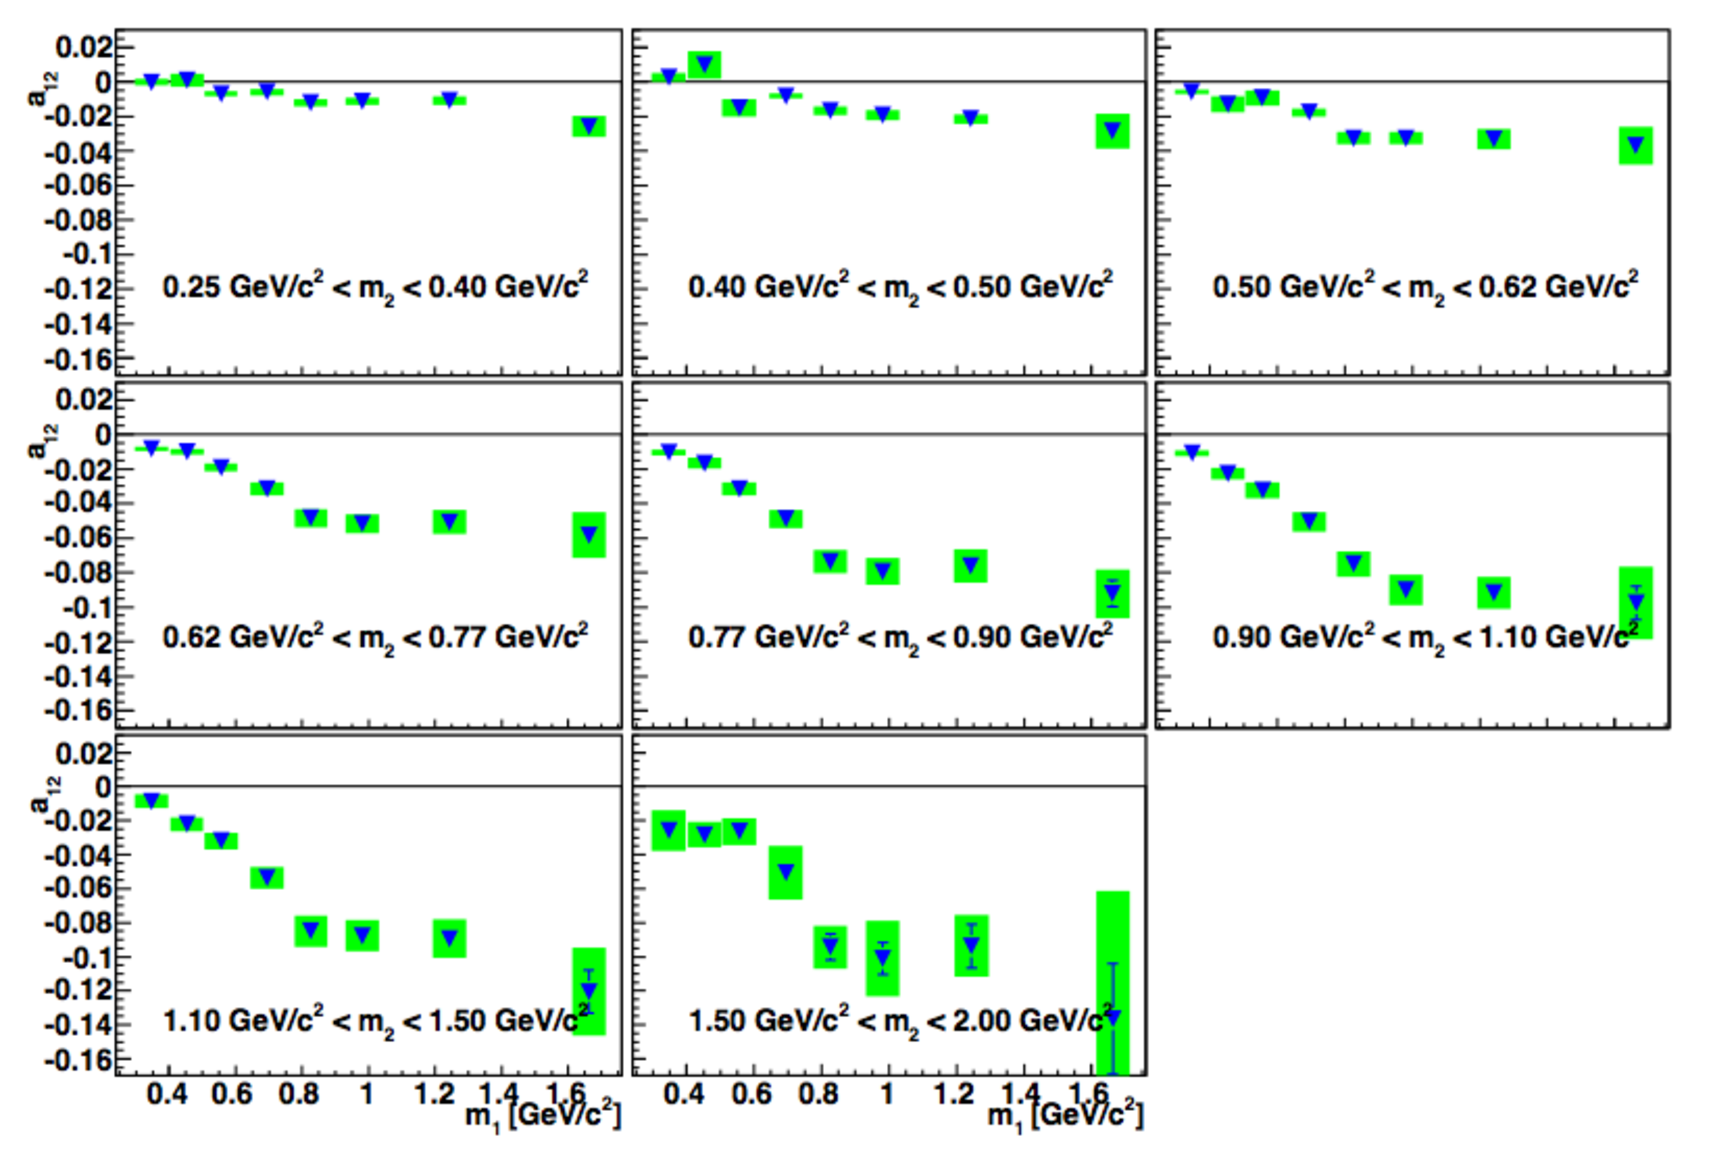
\includegraphics[width = 1\textwidth]{BelleAnnModulationM}
%\caption[Asymmetry seen in $e^-e^+$ annihilation at Belle]{Asymmetry in the number of back to back pion pairs seen at Belle plotted vs the invariant mass.}
%\label{fig:BelleMod}
%\end{center}
%\end{figure}
%
\section{Extracting IFF}
\label{sec:extractIFF}

The interference fragmentation function was extracted from the BELLE data using the replica method \cite{extractIFF}. N sets of replica data points were produced by shifting the experimentally determined data points by gaussian noise with the same width as the measured error. It was found that roughly 100 replicas were sufficient for the mean and standard deviation of the replicated data points to accurately reflect the measurements~\cite{extractIFF2}. 

By integrating over the antiquark jet, the Arturo-Collins asymmetry from equation \ref{eq:A-Casym} becomes proportional to
\begin{equation}
a_{12} \propto \frac{H(z_1,m_1;Q^2)}{D(z_1,m_1;Q^2)},
\end{equation}
where $D(z_1,m_1;Q^2)$ 
%is known from other unpolarized experiments. 
is estimated from PYTHIA calculations~\cite{Courtoy:2012ry}.
Restricting to only up and down quarks and requiring $n_u^\uparrow(Q^2) = -n_d^\uparrow(Q^2)$ gives
\begin{equation}
H(z_1,m_1;Q^2) = \frac{|\bm{R}|}{m_1}H_1^{\sphericalangle u}(z_1,m_1;Q^2)n^\uparrow(Q^2).
\end{equation}
Here the normalization $n^\uparrow(Q^2) = \int\text{d}z\int\text{d}m_1 H(z_1,m_1;Q^2)$. 

The theoretical value, $H^{TH}(z_1,m_1,Q^2;\{p\})$, is a complicated function\cite{RealEstValTrans} with parameter vector $\{p\}$ containing 9 parameters. These best-fit parameters were found for each replicated data set by minimizing the error
\begin{equation}
E_r^2(\{p\}) = \sum\limits_{ij} \left(H_{ij}^{TH}(z_1,m_1,Q^2;\{p\}) - H_{ij}(z_1,m_1;Q^2)\right)^2/\sigma_{ij}^2
\end{equation}
where index $i$ runs over the data points in invariant mass bin $j$. This results in $N=100$ different parameter vectors. A value of $H_1^{\sphericalangle u}(z_1,m_1;Q^2)$ is calculated from $H^{TH}(z_1,m_1,Q^2;\{p\})$ using the best fit parameters for each replica. The largest and smallest 16\% of the N calculated values are rejected leaving a 68\% confidence interval for the IFF.
\begin{equation}
R(z_1,m_1) = \frac{|\bm{R}|}{m_1} \frac{H_1^{\sphericalangle u}(z_1,m_1;Q^2)}{D_1^u(z_1,m_1;Q^2)}
\end{equation}
To visualize the IFF, a ratio, which can be seen as a function of $m_1$ for different values of the fractional energy $z$ in Fig.~\ref{fig:extractionIFF}, is constructed. Each colored band represents one of these values of z and corresponds to 68\% of the 100 replicas. Now armed with $H_1^\sphericalangle$, we can access the transversity in our analysis.  

 \begin{figure}
\begin{center}
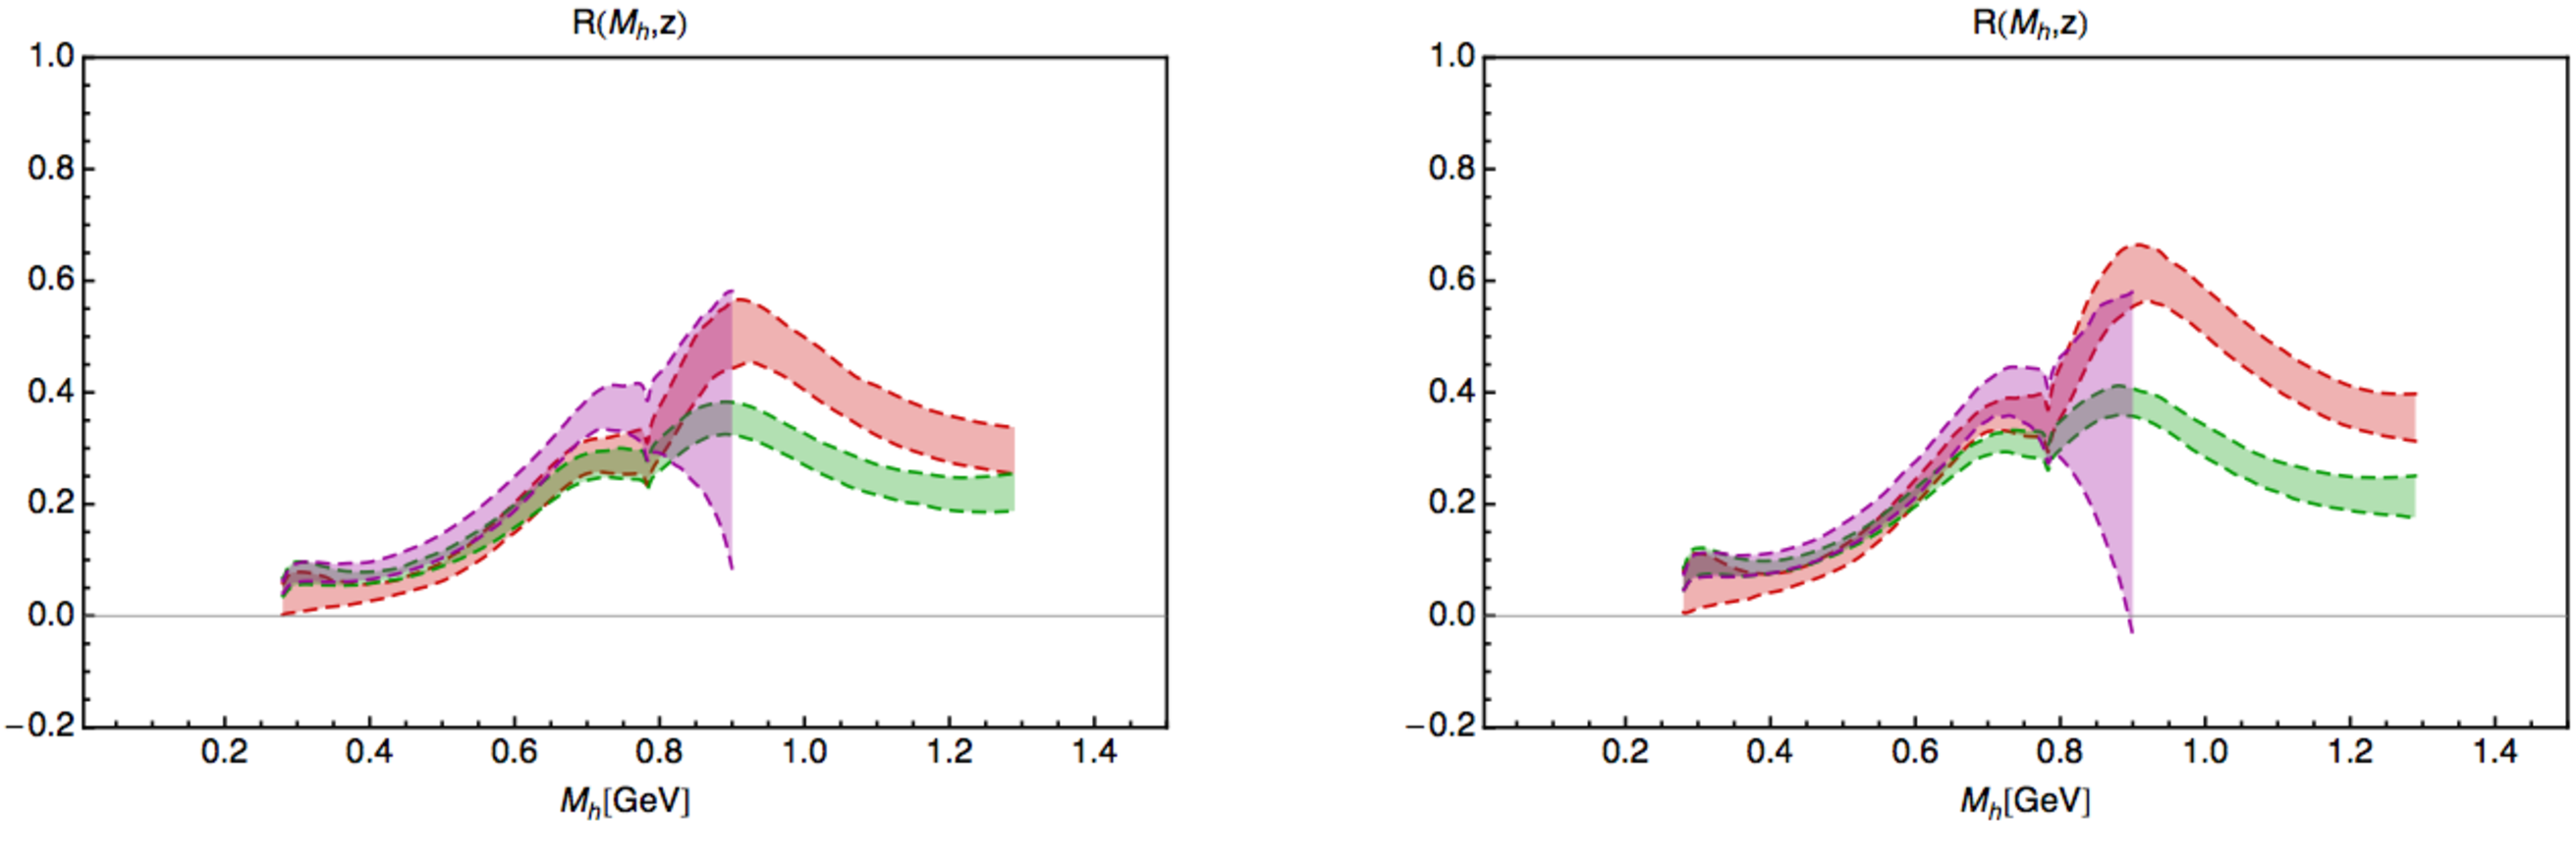
\includegraphics[width = .8\textwidth]{extractionIFF2}
\caption[Extraction of IFF from BELLE data]{The ratio $R(z,M_h)$ as a function of $M_h$ for three values of $z$: $z = 0.25$(purple), $z=0.45$(green), and $z=0.65$(red). The left panel is for $\alpha_s = 0.125$, and the right pannel is for $\alpha_s = 0.139$ \cite{RealEstValTrans}. Note: In their notation, $M_h = m_1$ is the invariant mass of the pion pair coming from the quark.}
\label{fig:extractionIFF}
\end{center}
\end{figure}




\section{Summary}

To leading order, the parton kinematics inside a proton can be described by three parton distribution functions (Fig.~\ref{fig:PDFs}); the unpolarized distribution function, $f_1(x)$, the helicity distribution function $\Delta f (x)$, and the transversity distribution function, $h_1(x)$ \cite{JaffeTONS}. The first two are well-known from DIS experiments, while the transversity distribution is not. Due to its chiral odd nature, a more different type of experiment is required to probe the transversity of partons inside the proton.  
\begin{figure}
\begin{center}
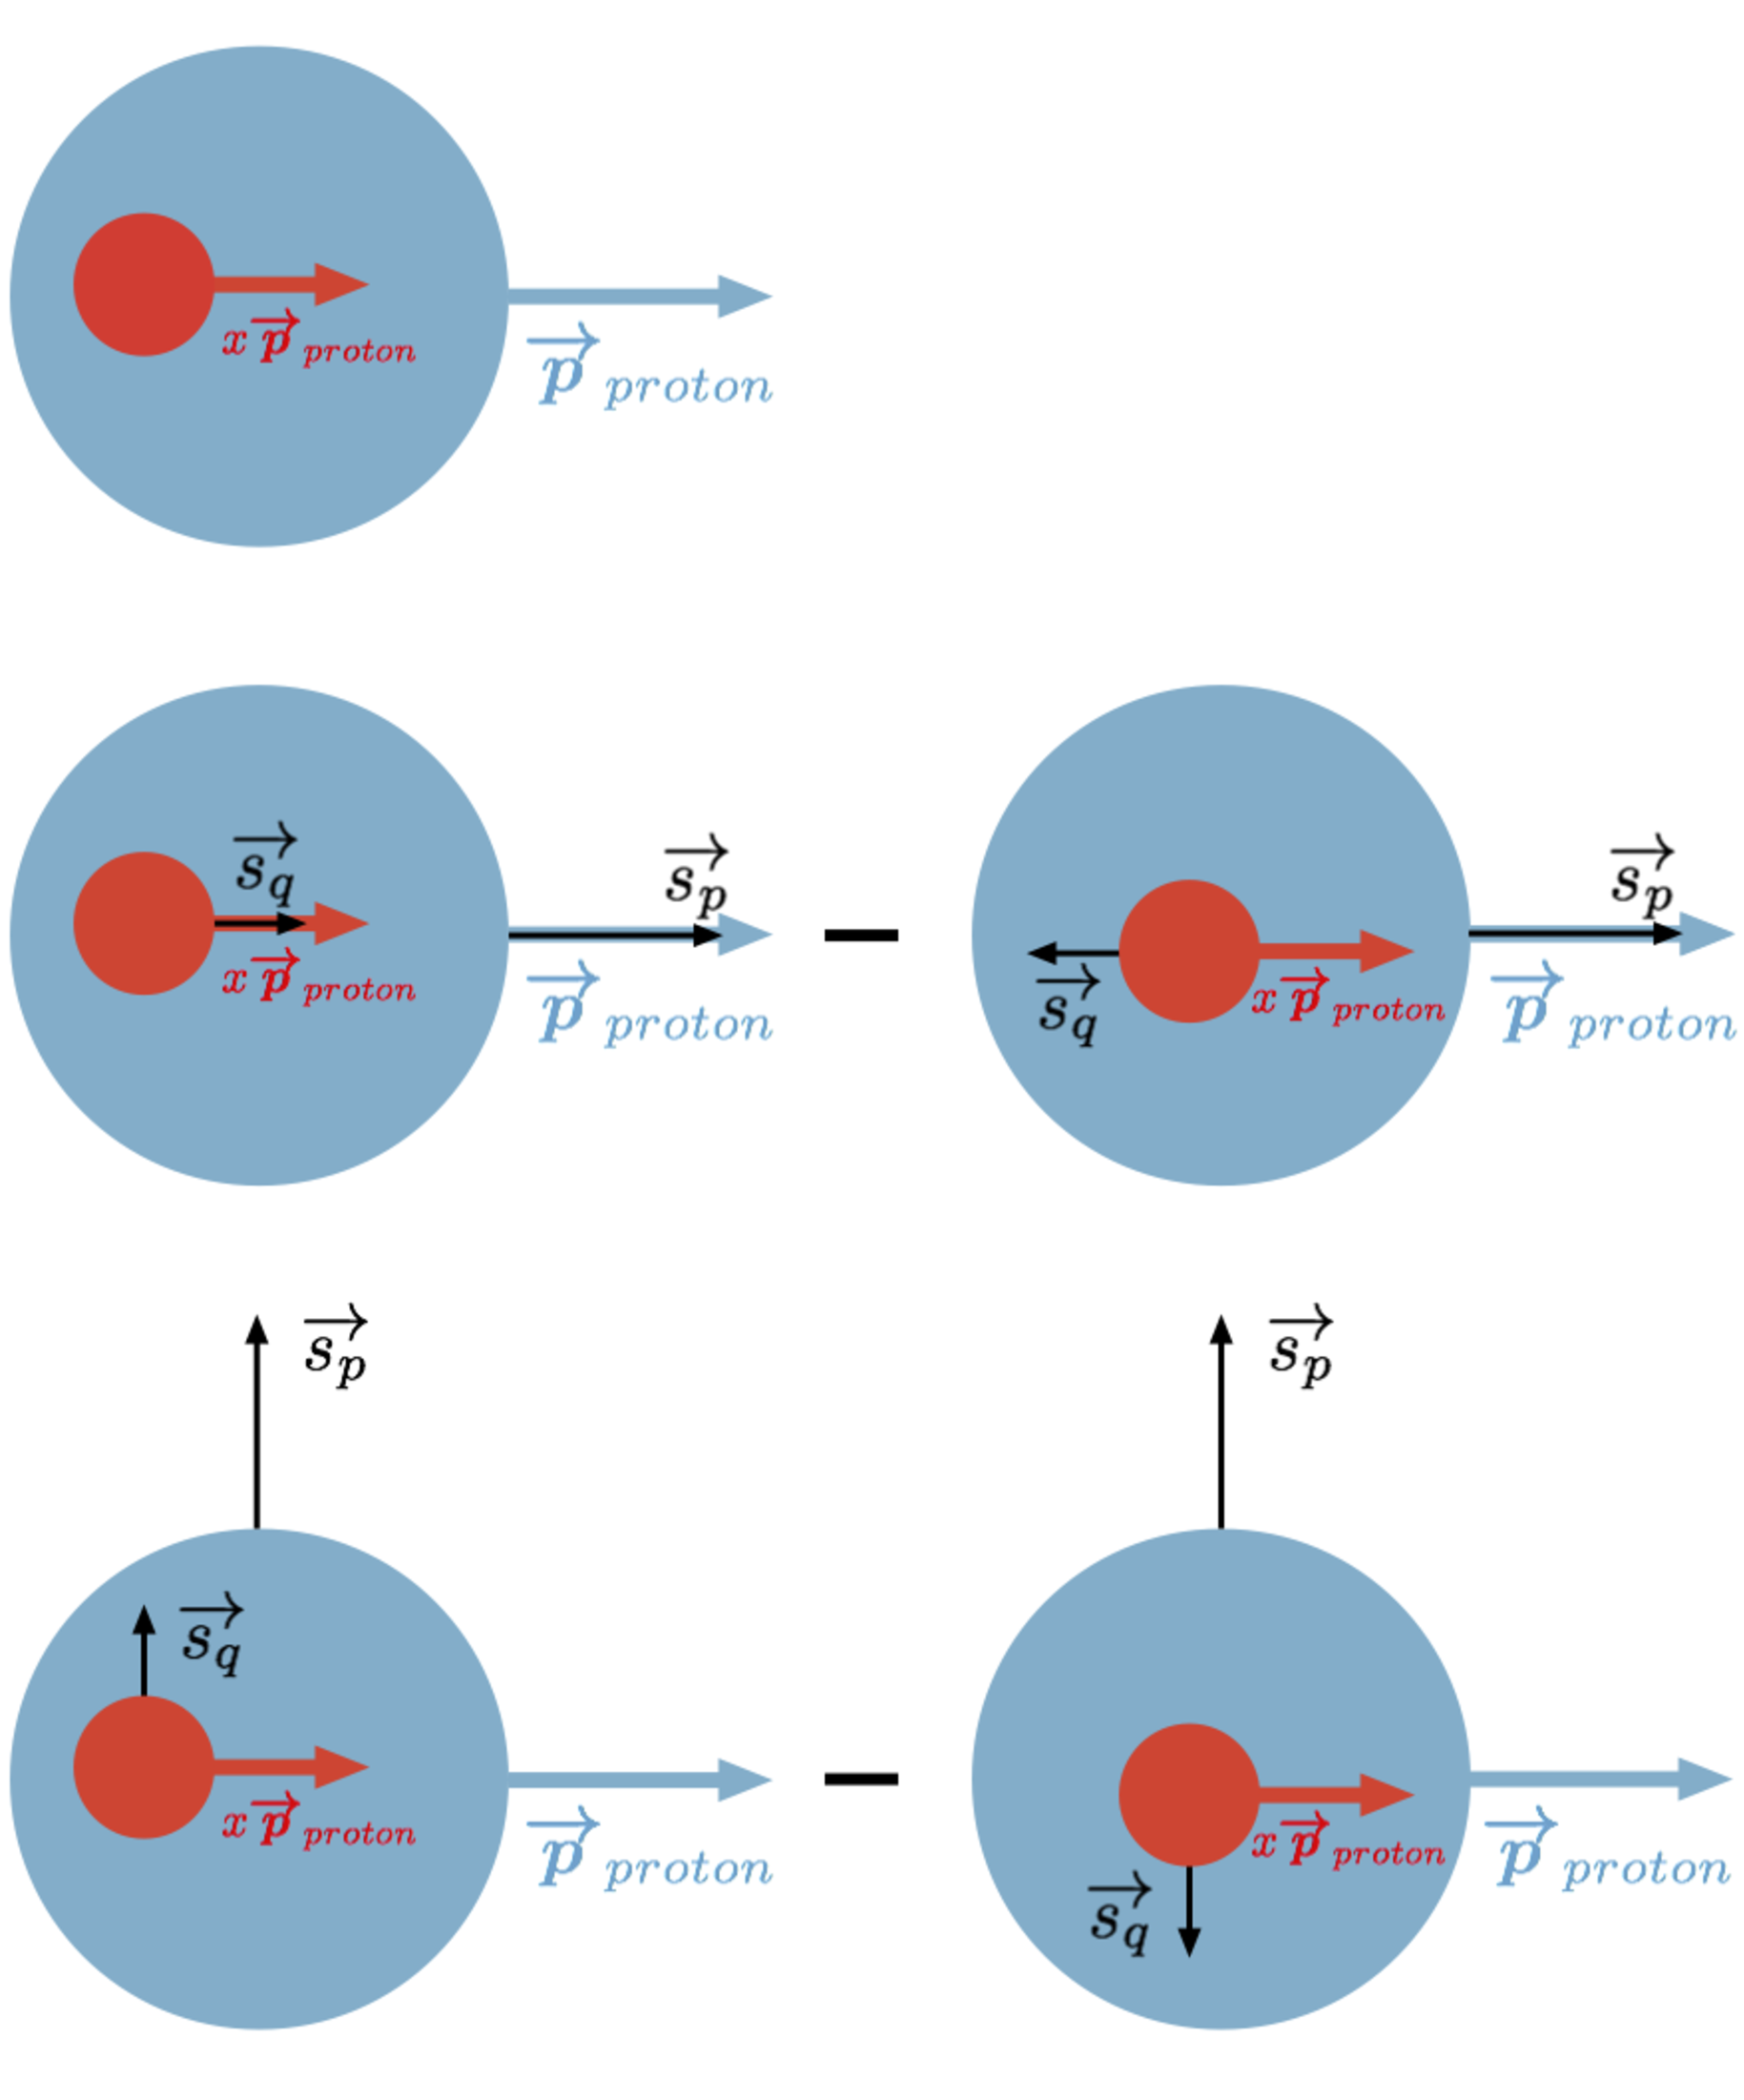
\includegraphics[width = .7\textwidth]{allDistsPic3}
\caption[Visual representation of unpolarized, helicity, and transversity distribution functions]{Top: Unpolarized distribution function $f_1(x)$ \\
Middle: Helicity distribution function $\Delta f(x)$ \\
Bottom: Transversity distribution function $h_1(x)$}
\label{fig:PDFs}
\end{center}
\end{figure}
%In the case of this thesis, a SIDIS experiment where two oppositely charged pions are detected will be utilized to probe transversity. 
%  I don't understand this sentence.  You have to make it clearer.
The IFF, which is used to describe how a transversely polarized quark fragments into a pair of oppositely charged pions is used as the second chiral odd object to pair with the transversity distribution function in order to construct an observable. A more detailed overview of the physics involved in the analysis will be given in chapter \ref{ch:theory}.

\chapter{RHIC and The STAR Experiment}

\section{The RHIC complex}
The Relativistic Heavy Ion Collider (RHIC), located at Brookhaven Nation Laboratory, is the only collider in the world that allows for spin-polarized proton collisions, as well as heavy nuclei collisions as the name suggests. The RHIC complex, shown in Fig.~\ref{fig:rhic}, is composed of a chain of accelerators which boost the energy in steps before finally injecting the particles into the large ring of RHIC. Heavy nuclei are first delivered to the Booster Synchrotron where they are accelerated to 95~MeV per nucleon. After which they are transferred to the Alternating Gradient Synchrotron (AGS). Here they are re-bunched into four bunches and accelerated to 10.8~GeV per nucleon, at which point they are injected into the RHIC ring and accelerated to their final energy. The highest energy RHIC can accommodate for heavy ions is 100~GeV per nucleon for gold nuclei. 
The story for protons is a little different. They are injected already spin polarized into the Booster Synchrotron from an older LINAC accelerator. From this point they are accelerated in the Booster and AGS before being injected into the RHIC storage ring. Here they are accelerated up to a maximum 250 GeV. 
In order to keep the spin polarization for the proton beam, special magnets called Siberian Snakes are used. These magnets flip the proton spin twice per revolution by 180 degrees in two orthogonal directions. 
The RHIC storage ring itself actually consists of two independent rings 3.8 km in circumference. This allows for the collisions of different species. The independent rings intersect at six locations. the STAR detector is located at one such intersection points\cite{RHICoverview}.

 \begin{figure}
\begin{center}
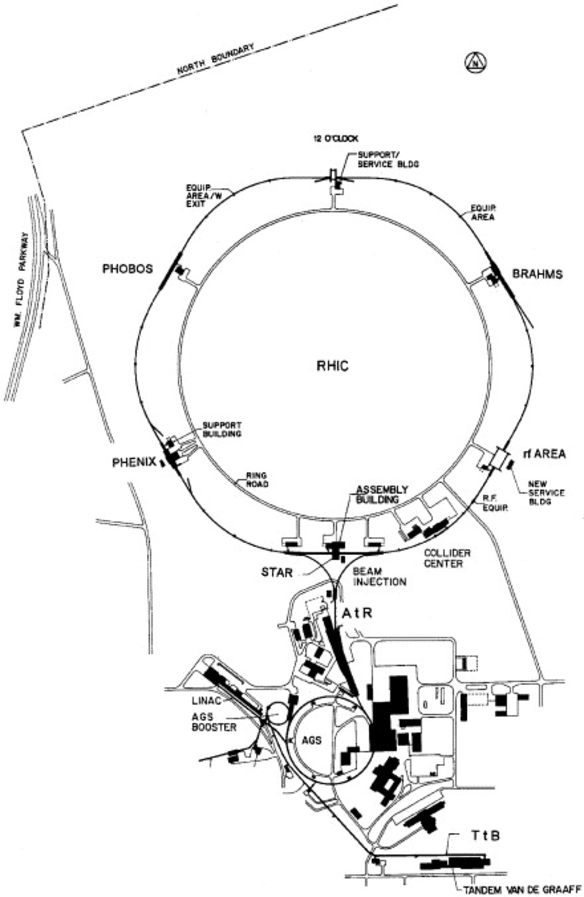
\includegraphics[width = 1\textwidth]{rhicBNL}
\caption[The RHIC complex]{The RHIC complex}
\label{fig:rhic}
\end{center}
\end{figure}
Acceleration of polarized protons in a circular accelerator can encounter resonant conditions which act to depolarize the beam. Special magnets called Siberian Snakes are used to overcome these depolarizing resonances. Each Siberian Snake consists of 4 superconducting helical dipole magnets. The role of the Siberian Snakes are to rotate the proton spin as shown in Fig.~\ref{fig:spinFlip}. If the spin rotation from the Siberian Snakes is much larger than that of the depolarizing resonances, the beam polarization is kept intact. In the RHIC ring, this is achieved with a pair Siberian Snakes in each ring which rotate the proton spin by 180 degrees in orthogonal directions for each orbit. The lower energy of the AGS calls for only partial Siberian Snakes which rotate less than 180 degrees, but still enough to maintain beam polarization \cite{ppCollider}.
Along with the Siberian Snakes, spin rotators are located at the experimental interaction points. These allow for the proton spin to be rotated from the transverse plane to the longitudinal plane before collisions, depending on the requirements of each  experiments \cite{ppCollider}.

Polarized protons start out as polarized $H^-$ ions produced from an optically pumped proton ion source (OPPIS).  This source produces $9\times 10^{11}$ polarized $H^-$ ions per 300$\mu$s pulse. These polarized ions are then accelerated to 200~MeV in the LINAC. They are then stripped of the electrons and injected into the Booster where they are further accelerated to 10.5~GeV. From here they are sent to the AGS and accelerated to 25~GeV. The final step is a transfer to RHIC for acceleration to a maximum of 250~GeV and storage \cite{ppCollider}.
\begin{figure}
\begin{center}
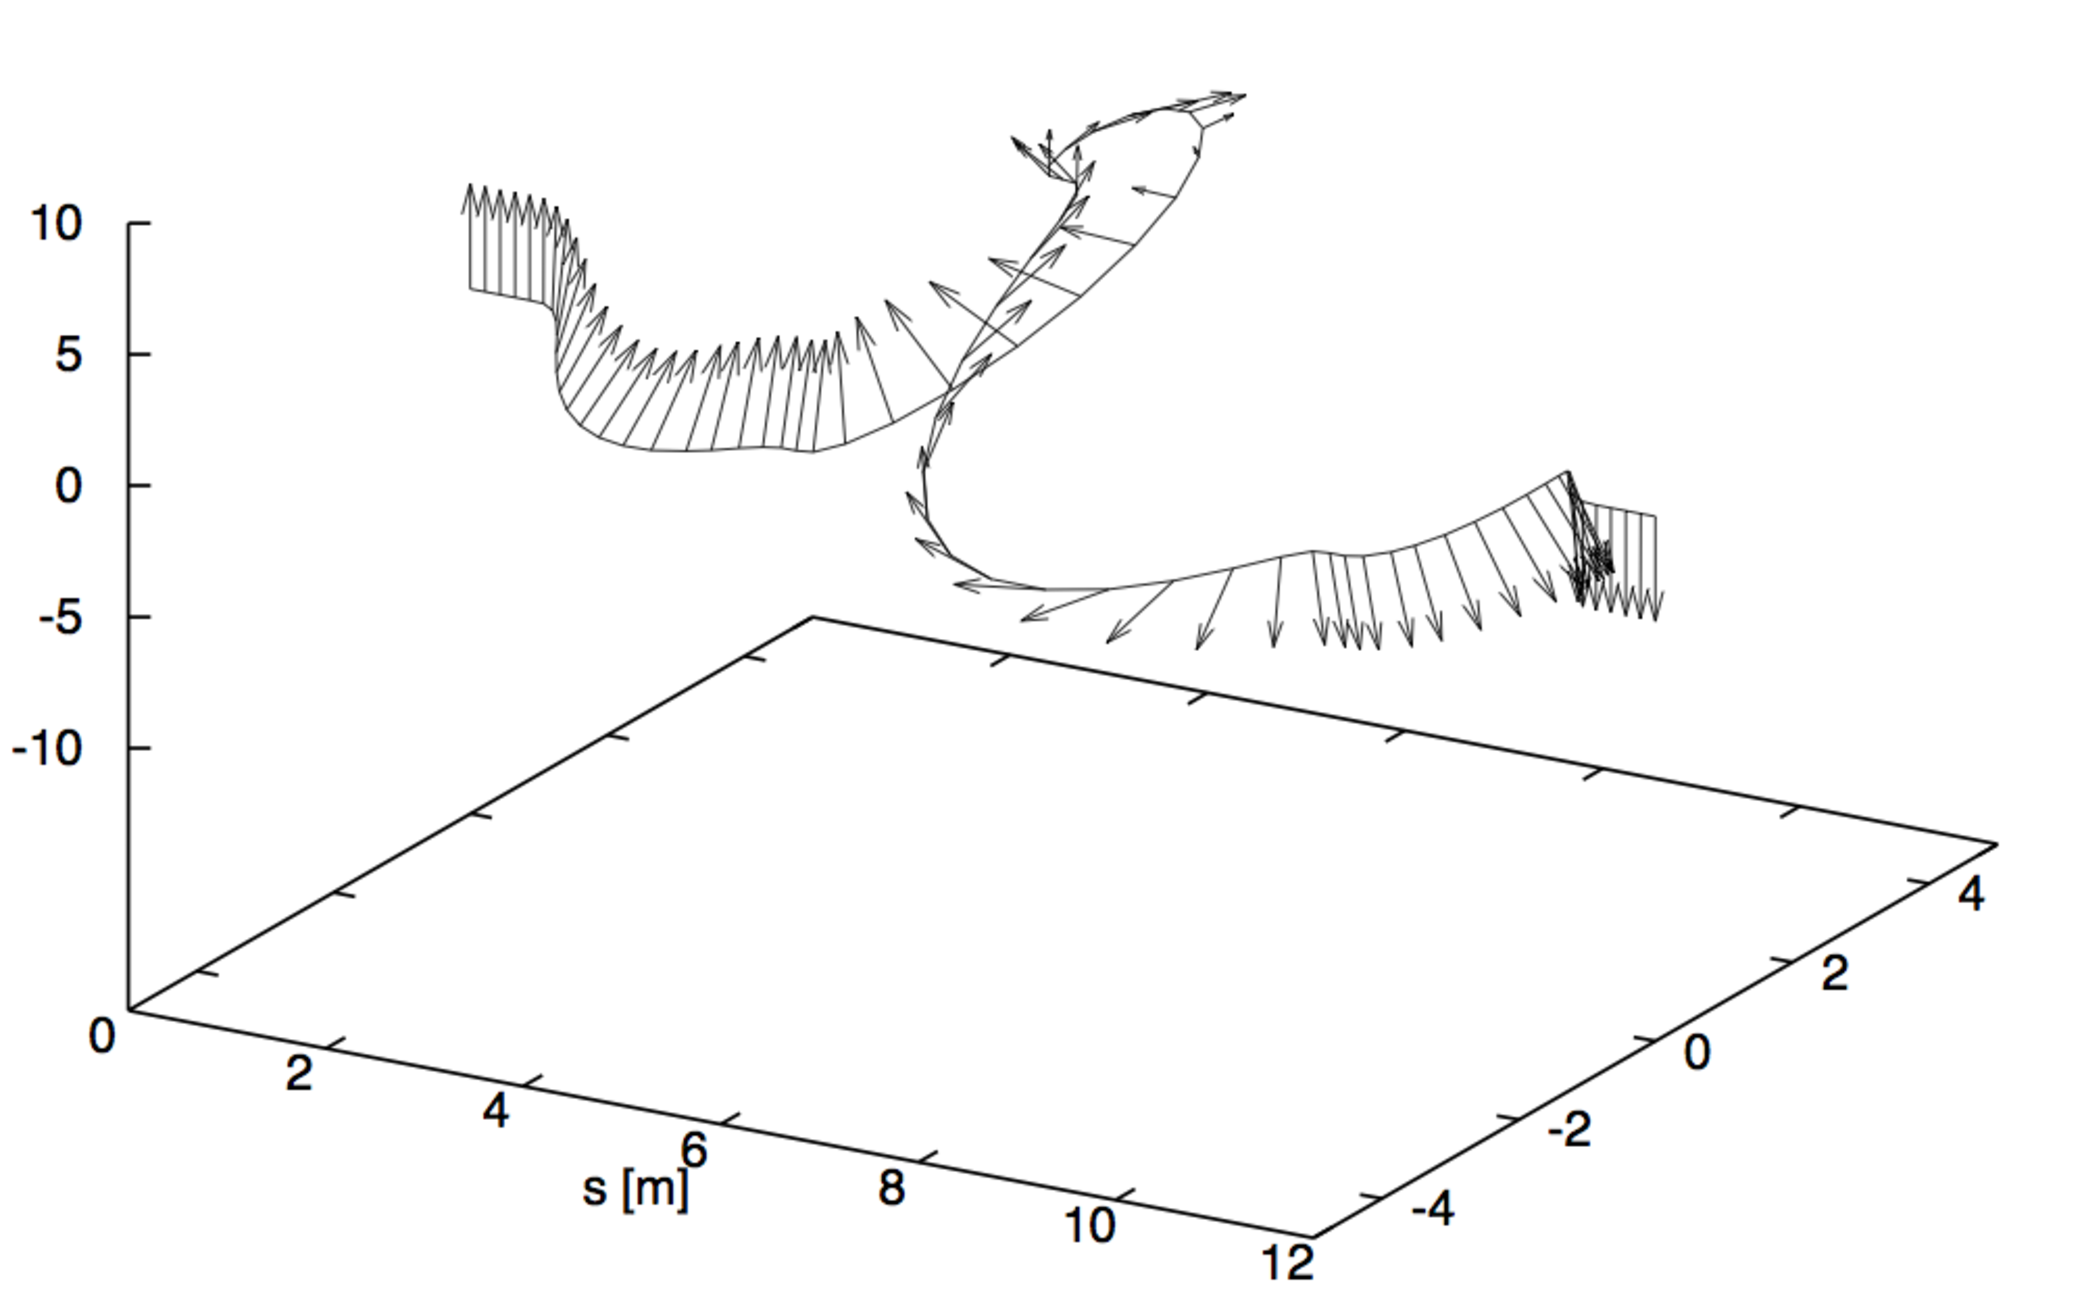
\includegraphics[width = 1\textwidth]{spinFlipFromPaper}
\caption[Spin flip by Siberian Snake]{180 degree proton spin flip by Siberian Snake}
\label{fig:spinFlip}
\end{center}
\end{figure}



\FloatBarrier

\section{The STAR Detector}
The Solenoid Tracker at RHIC (STAR) is located at the 6 o'clock position on the RHIC ring. It consists of several sub-detectors working in conjunction to detect, identify, and track particles. 

\subsubsection[TPC]{Time Projection Chamber}

\begin{figure}[h!]
\begin{center}
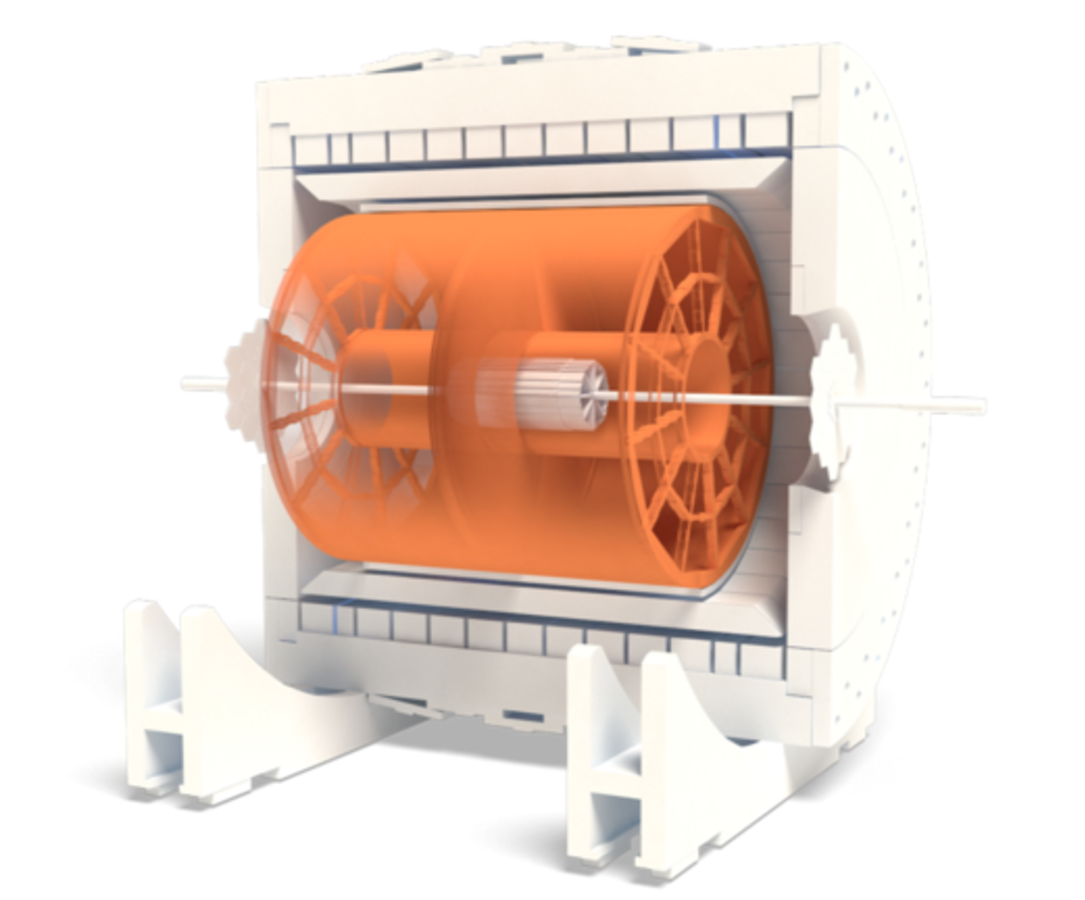
\includegraphics[width = .7\textwidth]{TPCfull}
\caption[STAR Time Projection Chamber]{STAR Time Projection Chamber}
\label{fig:tpcSchem}
\end{center}
\end{figure}

%
% There is a NIM volume dedicated to all the STAR detector
% subsystems.  Please refer to reader to these review articles.
%


One of they key detectors of STAR is the Time Projection Chamber (TPC). It is tasked with tracking particles, measuring momenta, and detecting ionization energy loss, $dE/dx$, to aid in particle identification. The TPC is the large cylindrical gas chamber covering $\pm1.8$ units of pseudorapidity around the interaction point. It's filled with a mixture of 10$\%$ methane and $90\%$ argon at a pressure of 2~mbar above atmospheric pressure. As a charged particle passes through the TPC, the gas is ionized, leaving a trail of electrons in it's wake. These electrons drift to the end caps of the TPC under a uniform electric field of about 135~V/cm where they are collected in a proportional chamber to record their drift time and location in the $r-\phi$ plane and along the $z$ direction. This information can be analyzed to reconstruct the track of the ionizing particle. The particle's path will curve due to the presence of STAR's magnetic field an amount proportional to the particles charge and it's velocity, allowing for the measurement of particle momenta, charge, and ionization energy loss.



%\begin{figure}
%\begin{center}
%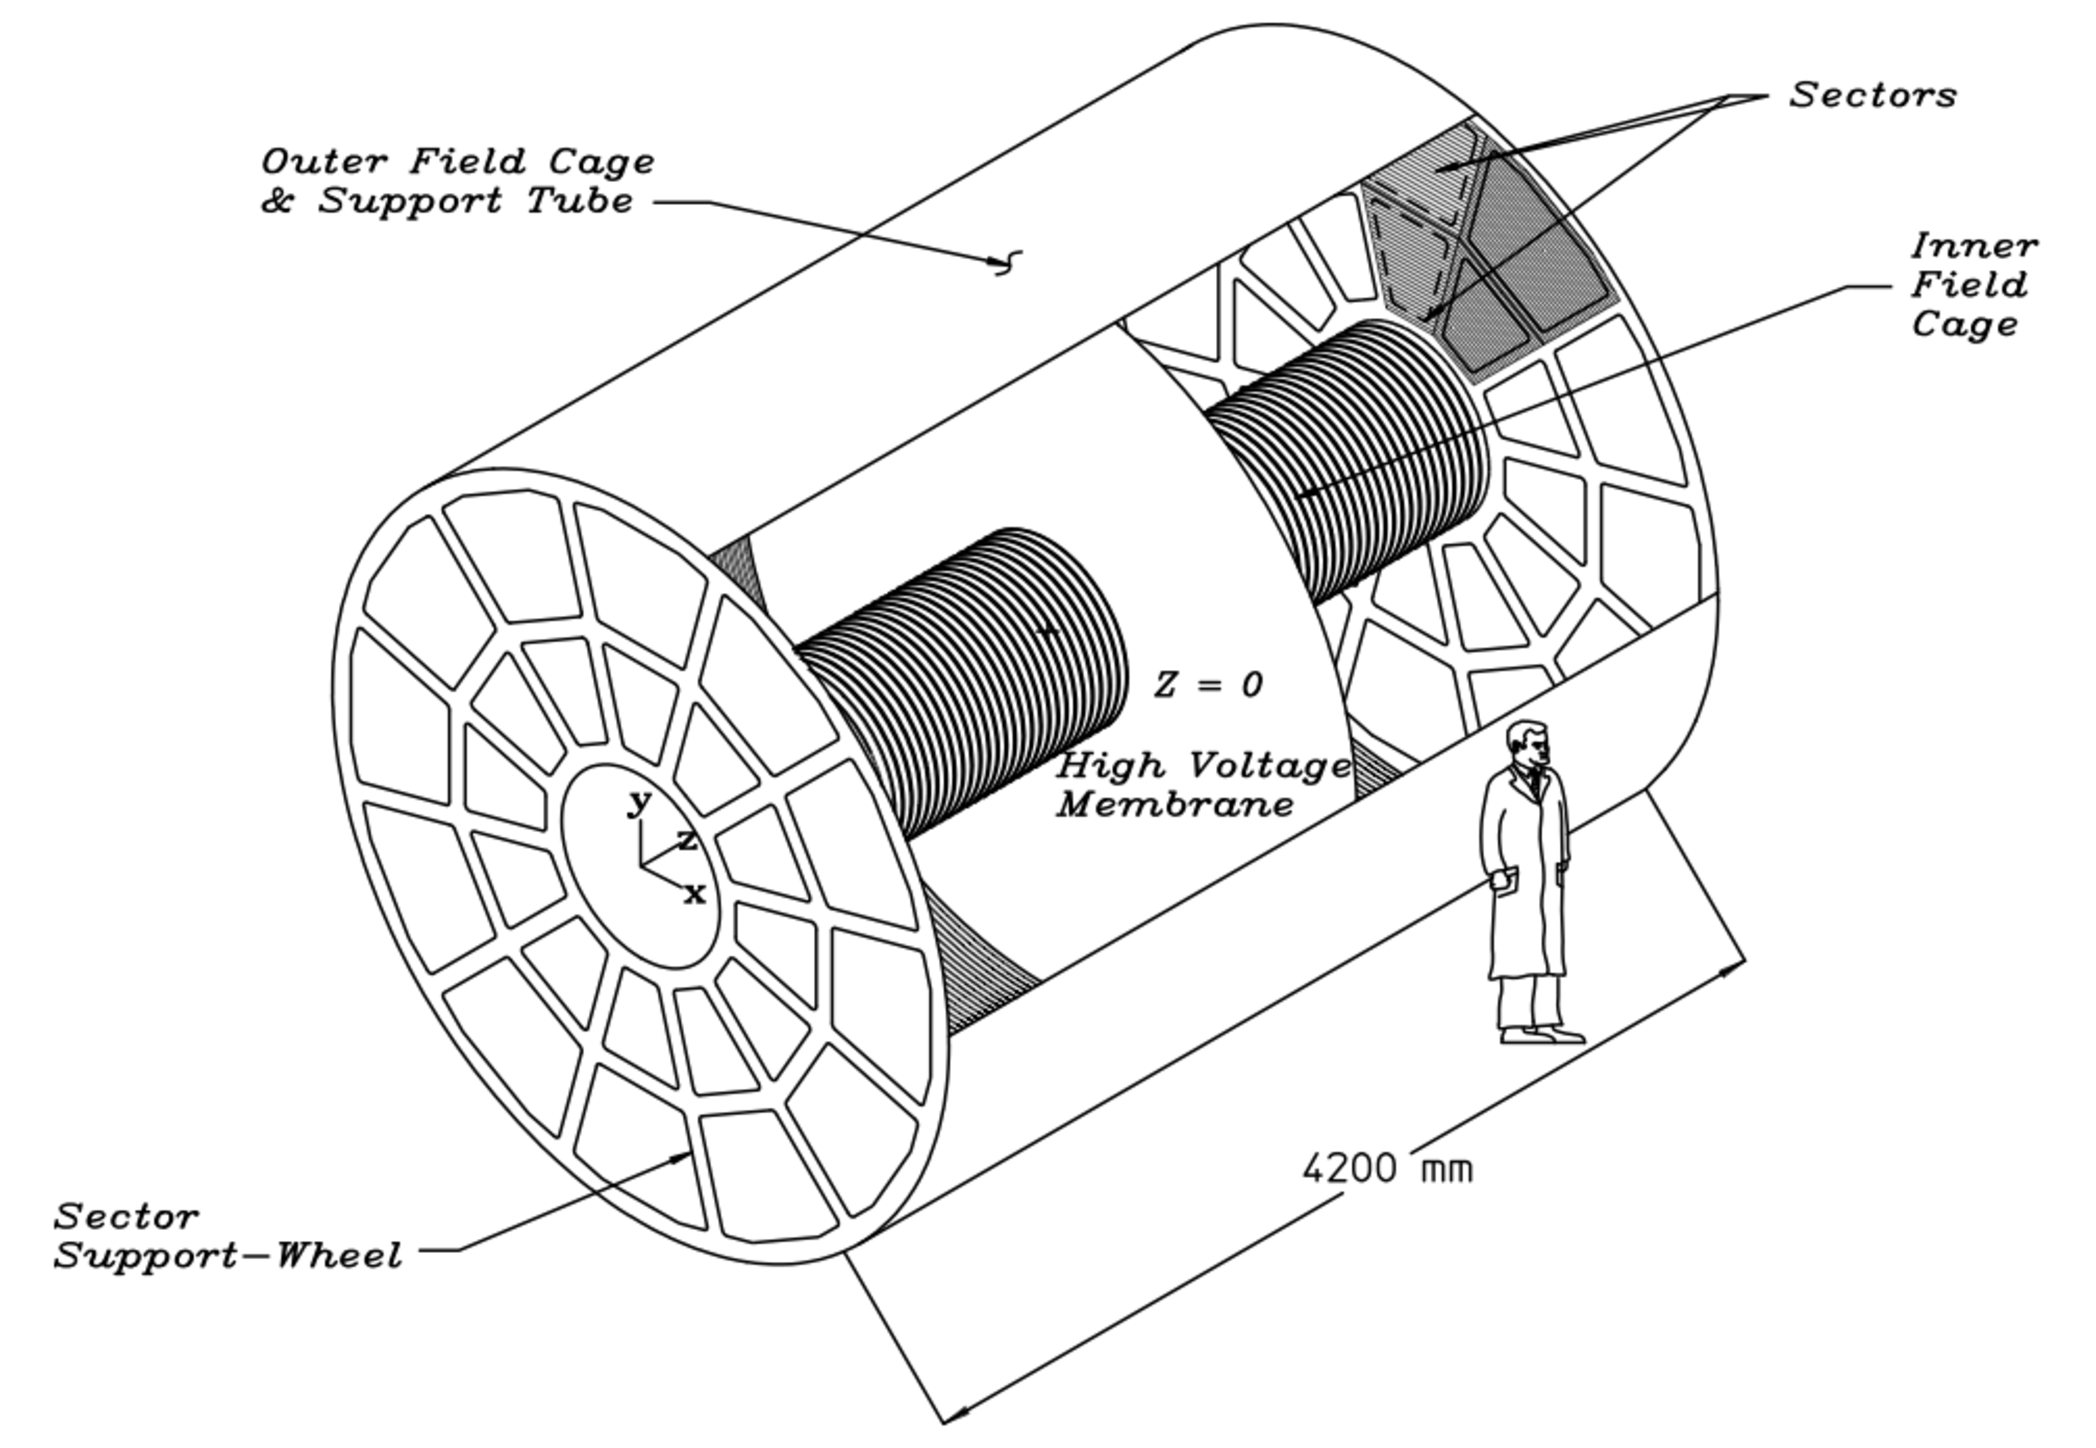
\includegraphics[width = 1\textwidth]{tpcSchem}
%\caption[STAR Time Projection Chamber]{STAR Time Projection Chamber}
%\label{fig:tpcSchem}
%\end{center}
%\end{figure}


At the center of the TPC is a central membrane which splits the TPC in two halves. This membrane is kept at 28 kV while the two end caps are at ground. A field cage is located around the TPC to create 182 equipotential slices in the TPC. This set up allows for a very uniform electric field to be kept.   

A mixture of 10$\%$ methane and $90\%$ argon is chosen for the TPC gas due to its relatively large drift velocity. This drift velocity also peaks at the operating electric field (135 V/cm) making it relatively unaffected by subtle fluctuations in the electric field.

The TPC gas drift velocity is calibrated with a laser system. Thirty six aluminum stripes are positioned on either side of the central membrane and are illuminated with an ultraviolet laser. This causes photo-ejection of electrons which drift to the end caps where they are read. The position of the aluminum stripes are known with such precision that the time it takes the ejected electrons to reach the end cap readouts, as well as the position they reach, can be used for calibration. 

The end cap is equipped with 12 modular sectors arranged covering 180 degrees in azimuth. These sectors are arranged like a clock with only 3~mm separating them. Each sector, shown in figure \ref{fig:tpcPad}, has a grid of readout pads and a wire proportional chamber consisting of three wire grids; a gating grid, a shield (or ground) grid and an anode grid. The gating grid is required to keep boundary conditions with the central membrane and field cage in order to achieve the uniform electric field, and is thus arranged to do so. It prohibits ions generated from avalanches on the anode wire from drifting back into the main TPC region and effecting the drift field. The anode wire plane is made up of 20$\mu$ wires aligned radially around the sector. This is to achieve maximum precision of the measurement of momenta from high momentum (straight) tracks. The anode grid is completed by wires in the other direction separated by 4 mm.

\begin{figure}
\begin{center}
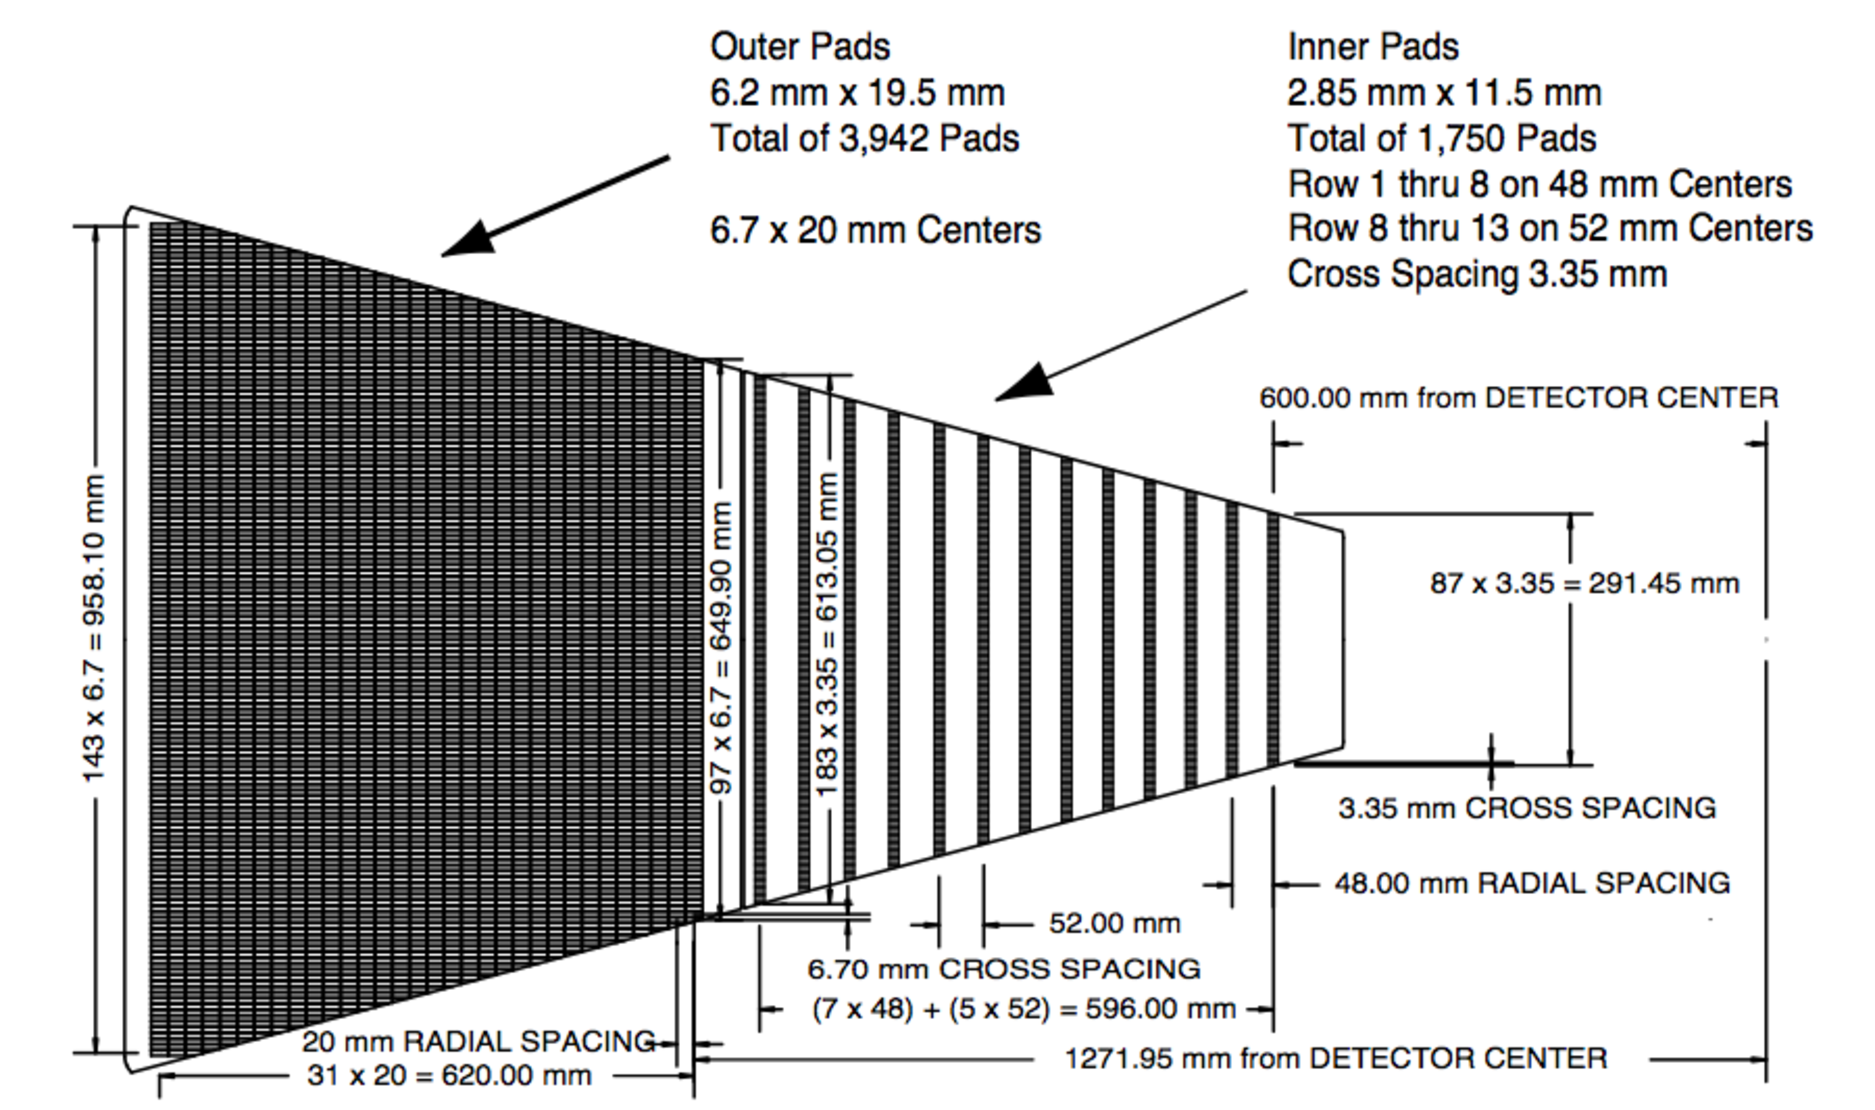
\includegraphics[width = 1\textwidth]{tpcPAD}
\caption[Anode sector of STAR TPC]{One of the 12 anode sectors of the TPC. The outer portion has densely packed pads, while the inner portion is composed of wider rows.}
\label{fig:tpcPad}
\end{center}
\end{figure}
As the drifting electrons reach the anode grid an avalanche occurs triggering a temporary image charge to be induced on the read-out pads. The width of each read-out pad is optimized to ensure that at least three read-out pads will share the signal from a single avalanche. This allows for the best centroid reconstruction. The grid of read-out pads is broken up into two sections. The outer portion of the grid has continuously packed read-out pads measuring 6.7~mm by 20~mm optimized for good $dE/dx$ resolution. These pads are located 4~mm behind the anode grid. The inner portion has smaller read-out pads measuring 3.35~mm by 12~mm optimized for good 2-hit detection. This helps with the large track density seen in the inner portion of the TPC. Due to the nature of the small pads, the space for electronics was limited. Unfortunately the electronic boards for read-out were not compact enough in the late 1990's when the TPC was constructed to fit in this available space. Because of this, it was impossible to have continuous radial coverage for the inner section as in the outer section. Instead they are arrange in strips as seen in Fig.~\ref{fig:tpcPad}. This arrangement prohibits the inner section to be much help in $dE/dx$ resolution \cite{TPC}.
\begin{figure}
\begin{center}
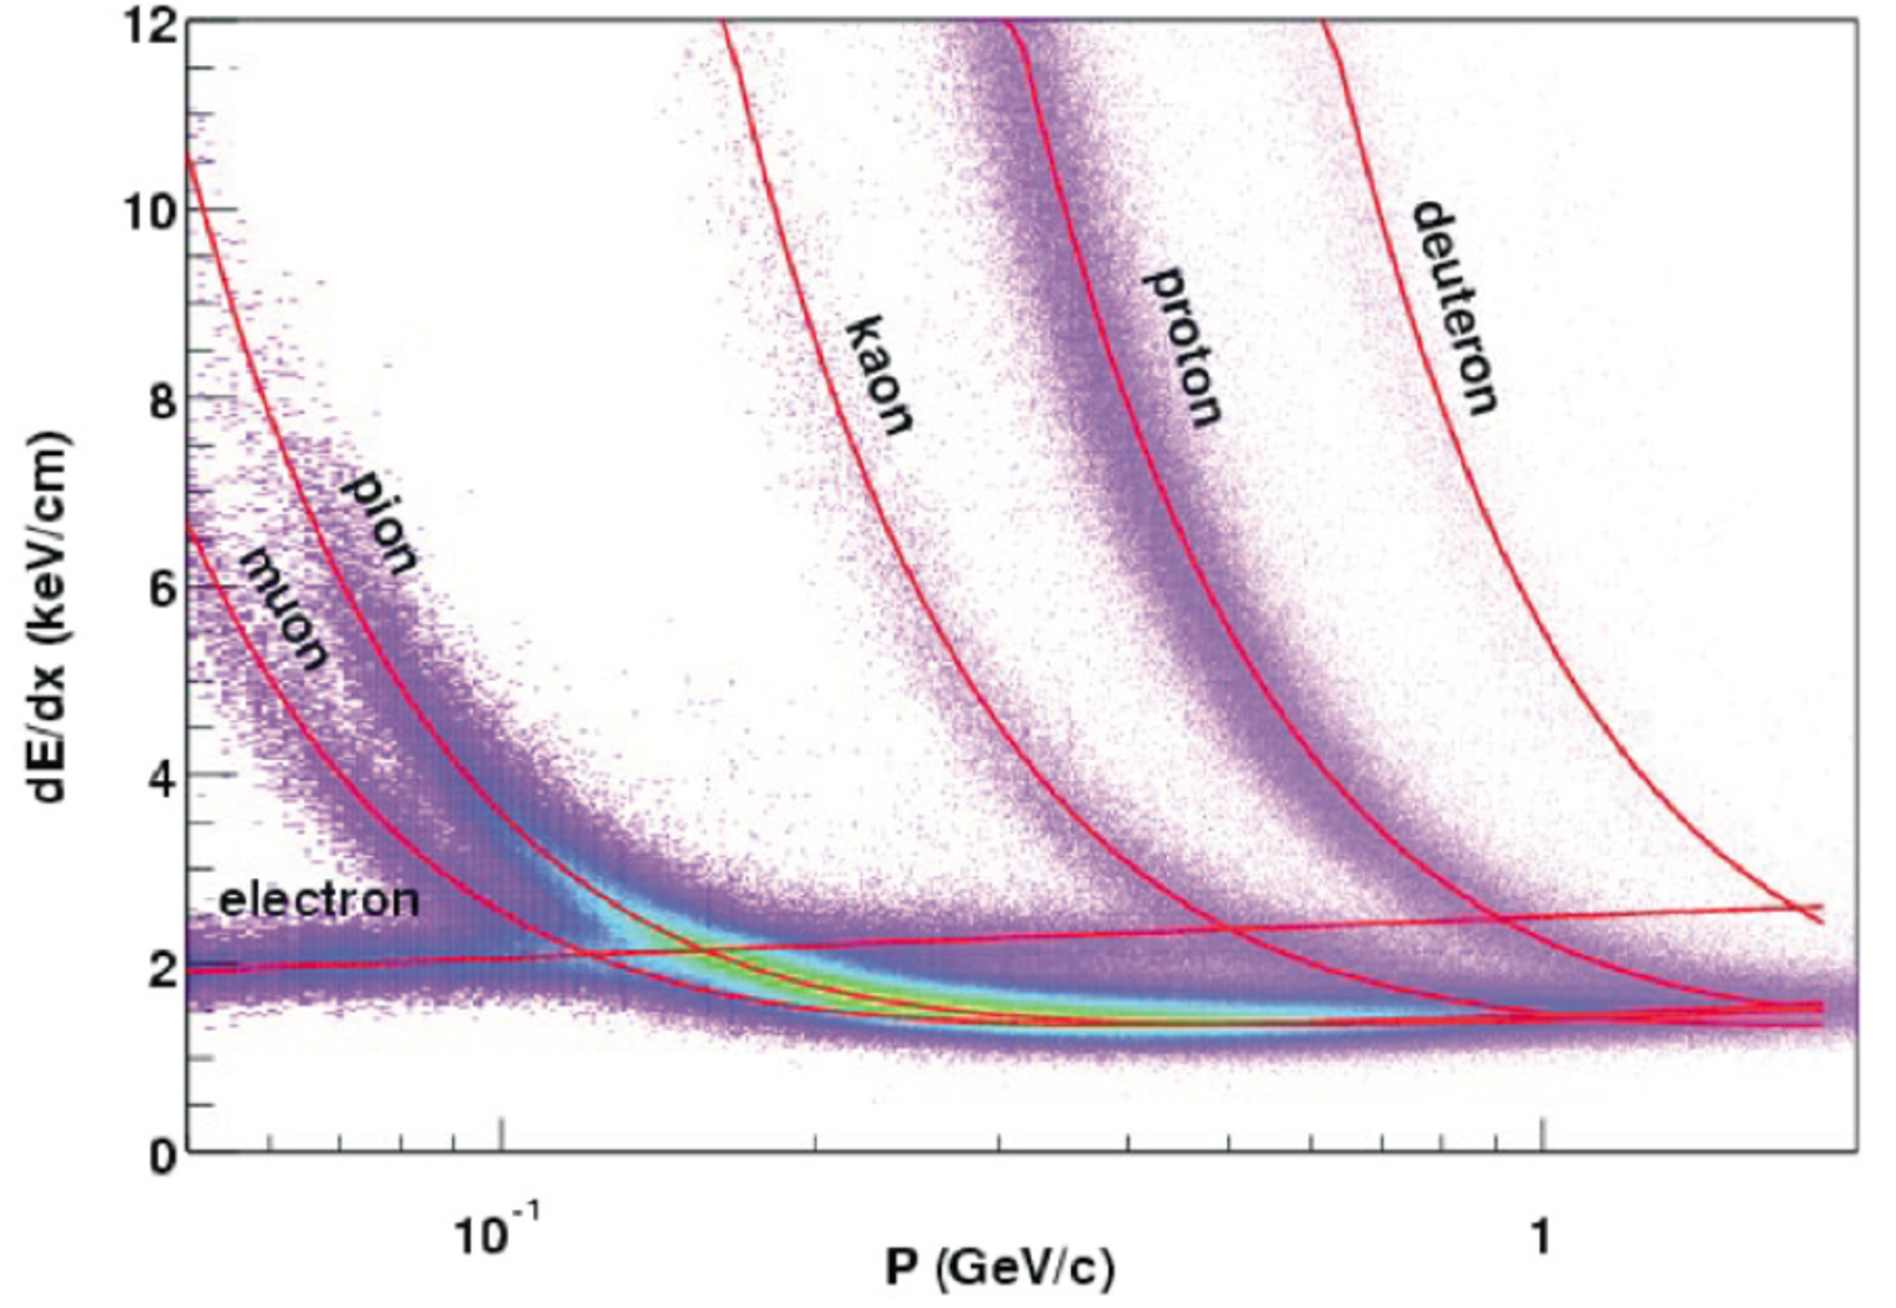
\includegraphics[width = 1\textwidth]{tpc_dEdx}
\caption[Ionization energy loss in TPC gas]{Ionization energy loss in TPC gas. Different species show different energy loss signature. This aids in particle identification.}
\label{fig:tpc_dEdx}
\end{center}
\end{figure}

\FloatBarrier
\subsubsection[BEMC]{Barrel Electromagnetic Calorimeter}


\begin{figure}[h!]
\begin{center}
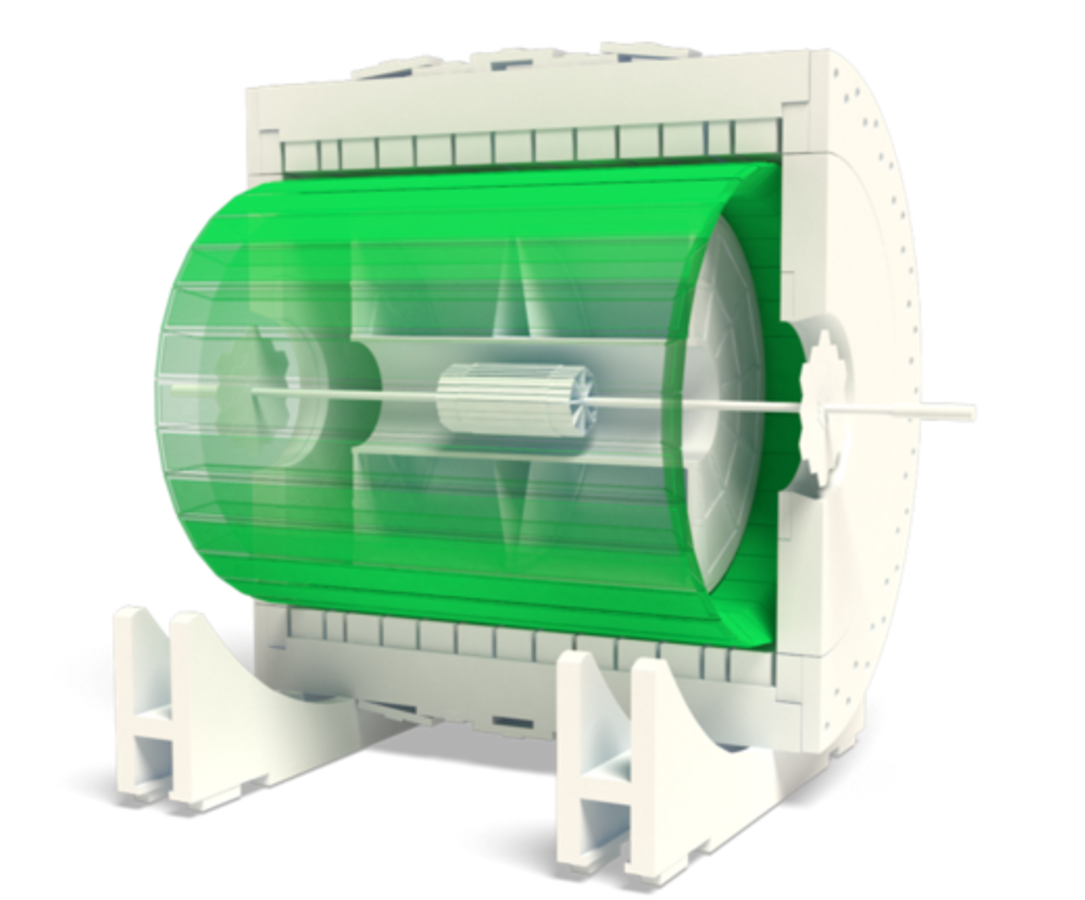
\includegraphics[width = .7\textwidth]{BEMC}
\caption[BEMC]{Barrel Electromagnetic Calorimeter (BEMC)}
\label{fig:BEMC}
\end{center}
\end{figure}


The Barrel Electromagnetic Calorimeter (BEMC) is a large array of lead and plastic scintillator sampling calorimeter sitting outside the TPC and inside the STAR magnet. At $\eta = 0$ the BEMC is roughly 20 radiation lengths thick allowing it to contain electromagnetic showers up to 60 GeV. Optical fibers are used to carry scintillation light from the BEMC array to outside the STAR magnet where it is fed into photomultiplier tubes (PMT).

The BEMC is composed of a total of 4800 towers, each one subtending 0.05$^\circ$ in $\phi$ and 0.05 units in $\eta$. A tower consists of 20 layers of 5~mm thick lead, 19 layers of 5~mm thick scintillator, and two layers of 6~mm thick scintillator. The tower geometry is projective toward the nominal interaction point, as seen in Fig.~\ref{fig:BEMC2}.  

The BEMC is equipped with a pre-shower detector which provide readings of the longitudinal shower development after 1 to 1.5 radiation lengths. Made up of the first two (6~mm) scintillating layers of the tower, the pre-shower detector aids in distinguishing between $\pi^0$ and $\gamma$ as well as between electrons and hadrons. Electrons will typically have a larger energy loss inside the BEMC than hadrons resulting in roughly 63\% of electrons showering before the pre-shower volume and 84\% by the middle of the pre-shower detector compared to only 3\% and 6\% for hadrons. The pre-shower detector consists of two 6 mm thick layers of scintillator instead of the 5~mm thick scintillator layers in the rest of the BEMC. 

The active scintillating layers, both pre-shower and regular, are made of Kuraray SCSN81 and light from each layer is carried out with wavelength-shifting fiber embedding into the scintillator layer. The scintillation light from each layer is transferred to a 2.1~m long optical fiber which carries it through gaps in the magnet steel to boxes containing an array of photomultipliers which are mounted outside the magnet. Here the light from all 21 layers in a tower, including the two pre-shower layers, are combined and fed into a single PMT. The pre-shower detector also passes a second sample of scintillation light from layers 1 and 2 to a separate PMT, this time not combined with light from any other layers.  

\begin{figure}
\begin{center}
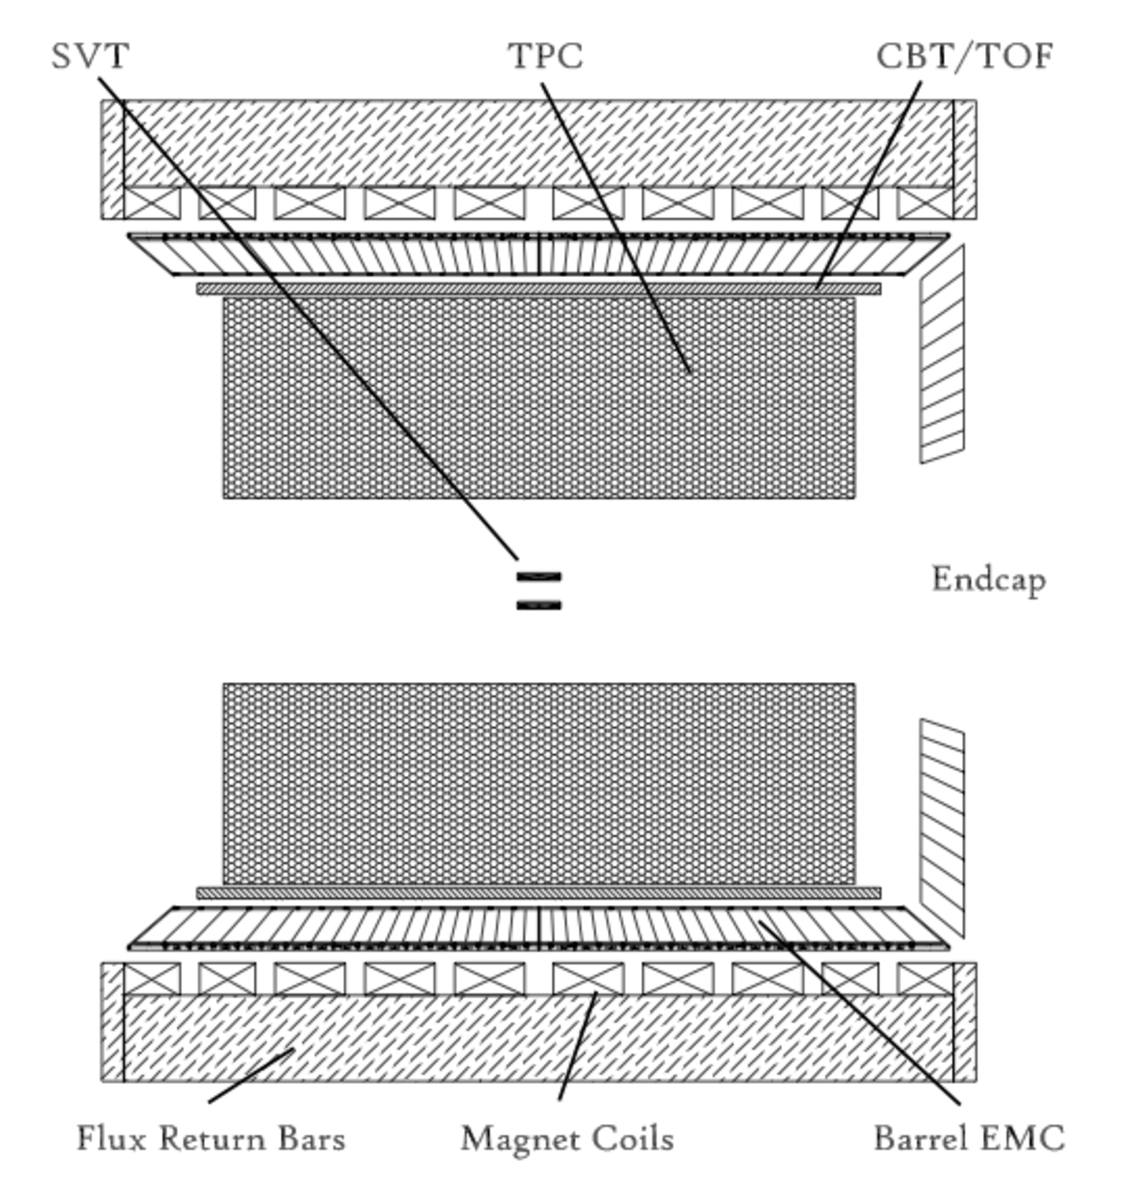
\includegraphics[width = .7\textwidth]{BEMC1}
\caption[Barrel Electromagnetic Calorimeter]{The BEMC is located outside the TPC but inside the STAR magnet and magnet flux return bars. The scintillation light is transported through gaps in the flux return bars where it is read out by PMTs.}
\label{fig:BEMC1}
\end{center}
\end{figure}

\begin{figure}
\begin{center}
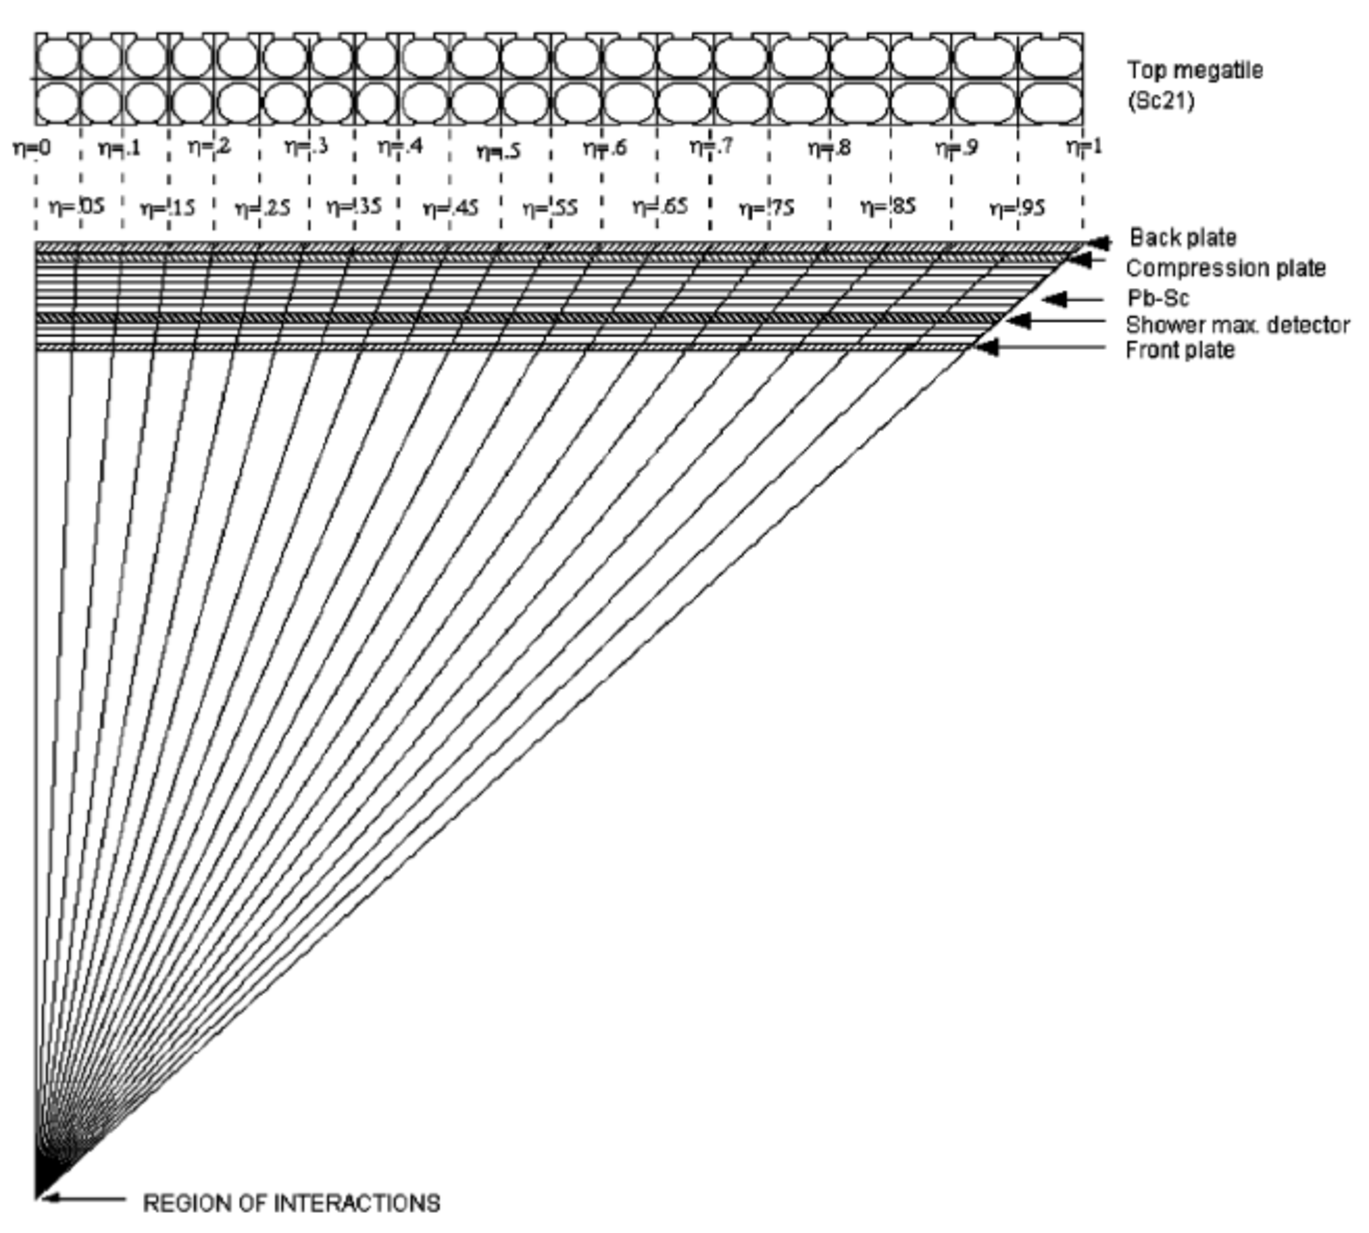
\includegraphics[width = .7\textwidth]{BEMC2}
\caption[Barrel Electromagnetic Calorimeter 2]{Each geometrical shape of each tower of the BEMC is projective, back to the nominal interaction region of STAR. The shower max detector as well as the individual scintillator/lead layers are shown.}
\label{fig:BEMC2}
\end{center}
\end{figure}

Some neutral particles, such as $\pi^0$, $\rho$, $etc.$ do not ionize the TPC gas, but may decay to daughter particles which interact electromagnetically. The BEMC is tasked with providing spatial resolution of such species. Instead of making the size of each tower of the BEMC comparable to the Moliere radius in the lead-plastic scintillator, a shower maximum detector (SMD) is added into the BEMC for spatial resolution. The SMD, set at about 5.6 radiation lengths at $\eta=0$, is composed of an aluminum plate with channels on either side. As seen in Fig.~\ref{fig:SMD2}, a 50$\mu$m gold-plated tungsten anode wire lies in each channel. The wires run along the barrel. As $e+e^-$ pairs generated in the electromagnetic shower enter the gas volume, a large ionization signal is generated. Detection strips are located on the top and bottom faces of the aluminum plate. One set of strips runs parallel to the wires and provides the spatial distribution of the shower in the $\eta$ direction. The other set, running perpendicular to the wires provides the spatial distribution in the $\phi$ direction. A schematic of this is shown in Fig.~\ref{fig:SMD1}. Together they give a full description of the shower position \cite{BEMC}.

\begin{figure}
\begin{center}
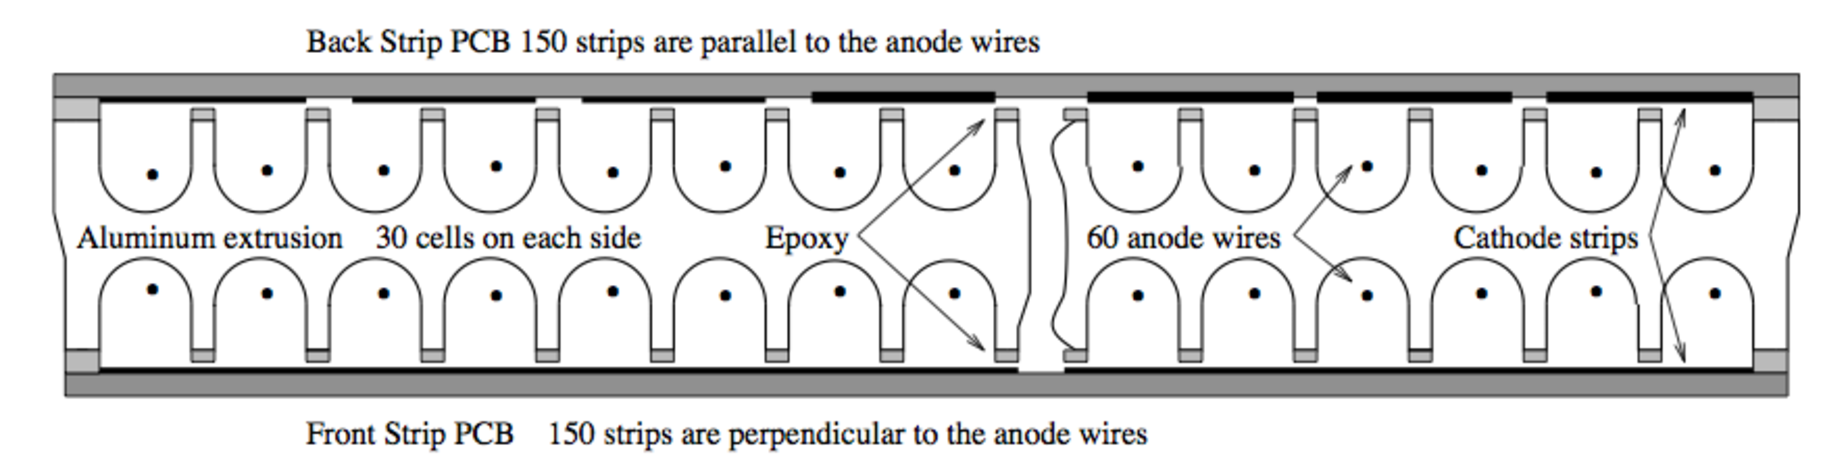
\includegraphics[width = .6\textwidth]{SMD2}
\caption[Shower Maximum Detector cross sectional view]{Cross sectional view of the shower max detector. Aluminum extrusion in the center containing two sets of anode wires. Cathode strips on the top and bottom face run either parallel or perpendicular to the anode wires.}
\label{fig:SMD2}
\end{center}
\end{figure}

\begin{figure}
\begin{center}
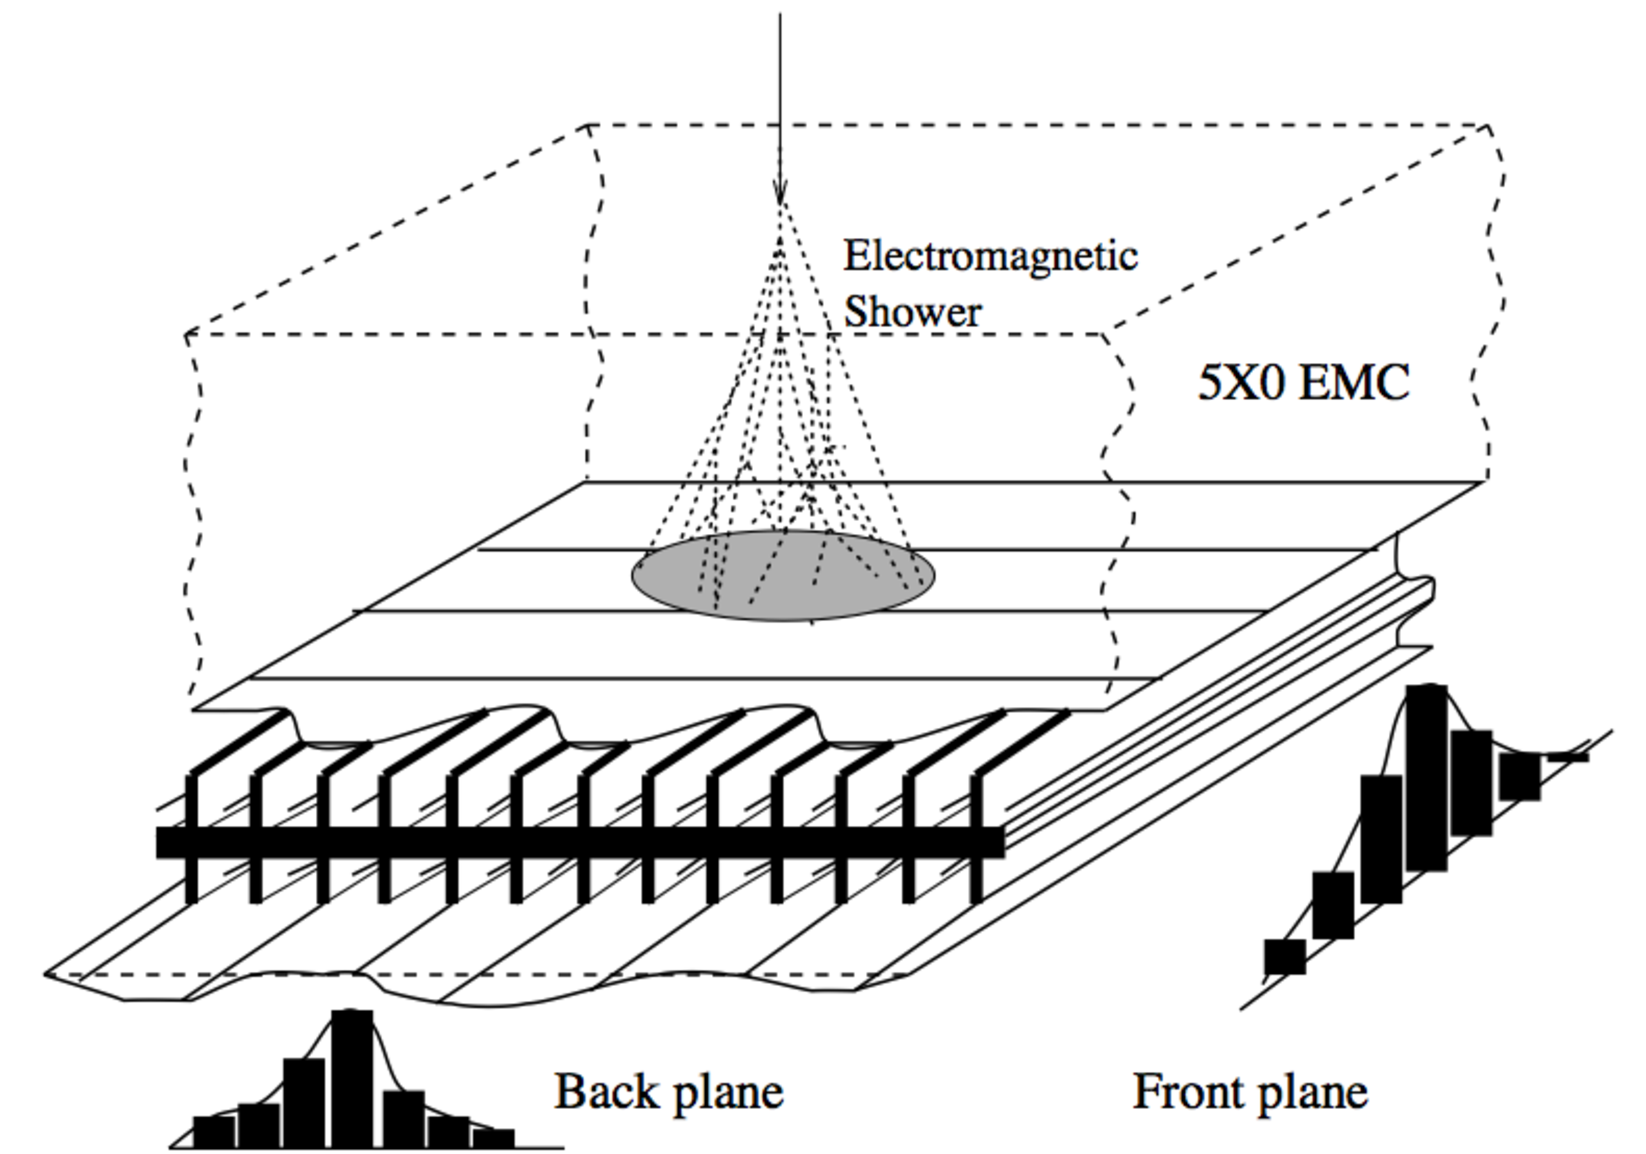
\includegraphics[width = .6\textwidth]{SMD1}
\caption[Spatial reconstruction in the SMD]{Schematic of spatial reconstruction in SMD. The cathode strips on the top and bottom faces read the induced charged in the $\phi$ and $\eta$ directions separately.}
\label{fig:SMD1}
\end{center}
\end{figure}

\FloatBarrier
%\subsubsection[EEMC]{Endcap Electromagnetic Calorimeter}

\subsubsection[TOF]{Time of Flight}

STAR has a time-of-flight system for particle identification. The system is composed of two different detectors, the Time of Flight Patch Detector (TOF) and the Vertex Position Detector (VPD).  Together these detectors allow for direct 2$\sigma$ $\pi$/$K$/$p$ identification for track momenta up to about 1.7 GeV/$c$.

The VPD is responsible for starting the clock of the time-of-flight system. It consists of two segmented plastic scintillator detectors, one on either side of the STAR interaction region, at a distance of 5.6 m from the center of the STAR detector. Both are positioned very close to the beam pipe and detect very forward, high energy photons produced in the collision. The average of the start time for both detectors to see this photon pulse is declared the ``start time" for the event. The scintillation light is read out by PMTs. 
%The magnetic field strength near the VPD is on the order of a few hundred Gauss. Because of this the PMTs are shielded on the sides with a steel outer shield, a nickel-Iron alloy intermediate shield, and finally a foil inner shield. They are also shielded from the front with a lead face sheet and a steel cap. A pVPD detector element is shown in Fig.~\ref{fig:vpdDetector}. This is mounted to the beam pipe support structure as shown in Fig.~\ref{fig:vpdAssembly}.    

%\begin{figure}
%\begin{center}
%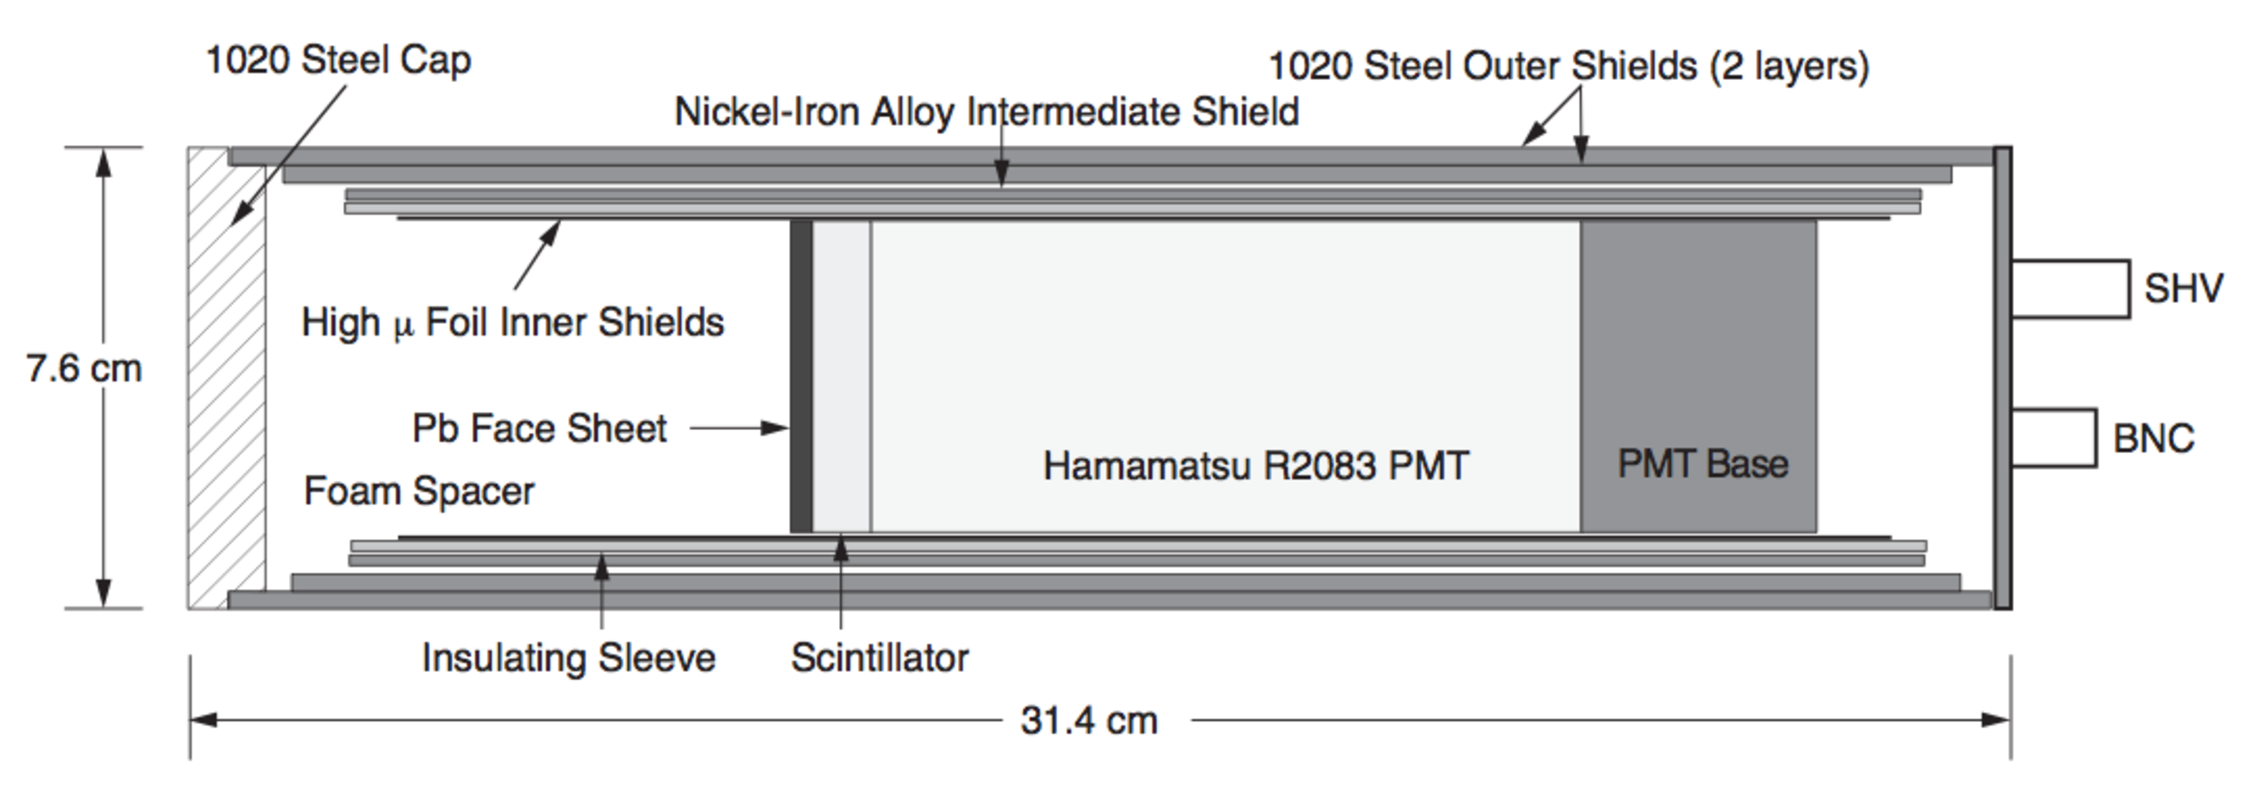
\includegraphics[width = .8\textwidth]{vpdDetector}
%\caption[VPD detector element]{A cross section of a VPD detector element.}
%\label{fig:vpdDetector}
%\end{center}
%\end{figure}

\begin{figure}
\begin{center}
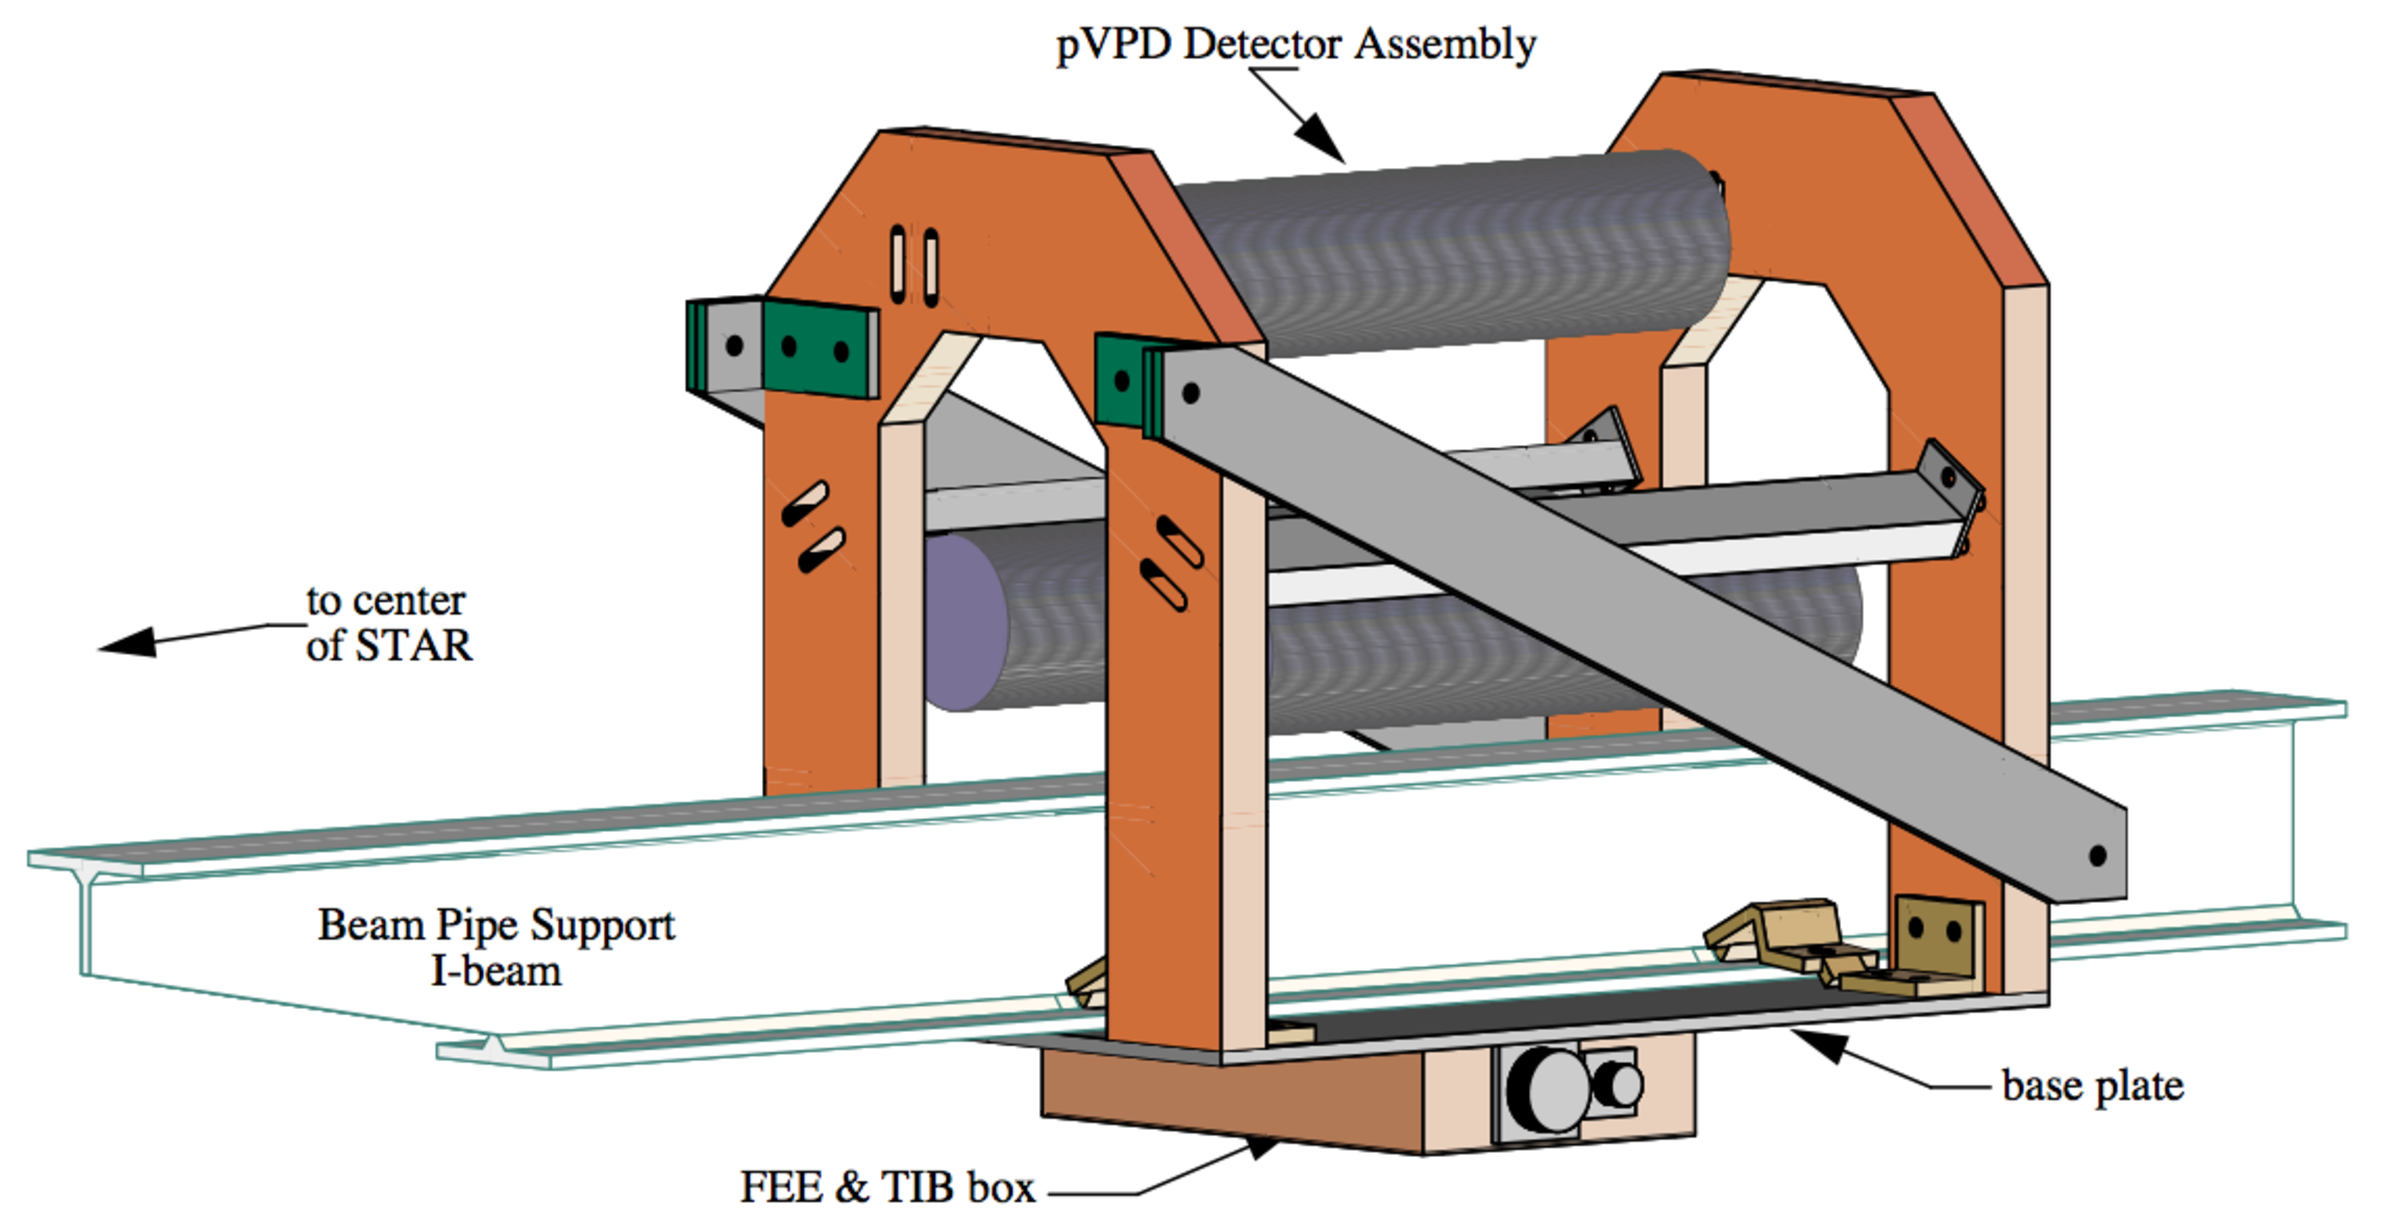
\includegraphics[width = .6\textwidth]{vpdAssembly}
\caption[VPD Assembly]{The VPD detector is mounted in the assembly.}
\label{fig:vpdAssembly}
\end{center}
\end{figure}

The VPD starts the clock for the event and the TOF stops it. The TOF uses the multi-gap resistive plate chamber (MRPC) technology developed by the ALICE group. The MRPC, shown in Fig.~\ref{fig:MRPC}, is a stack of resistive plates with uniform gas gaps in between. Applying a high voltage to electrodes on the outer plates creates a strong electric field in each gap. An avalanche is generated in the gaps when a charged particle passes through. Copper pickup pads located outside the electrodes are used to read out the signal \cite{largeAreaTOF}. 
\begin{figure}
\begin{center}
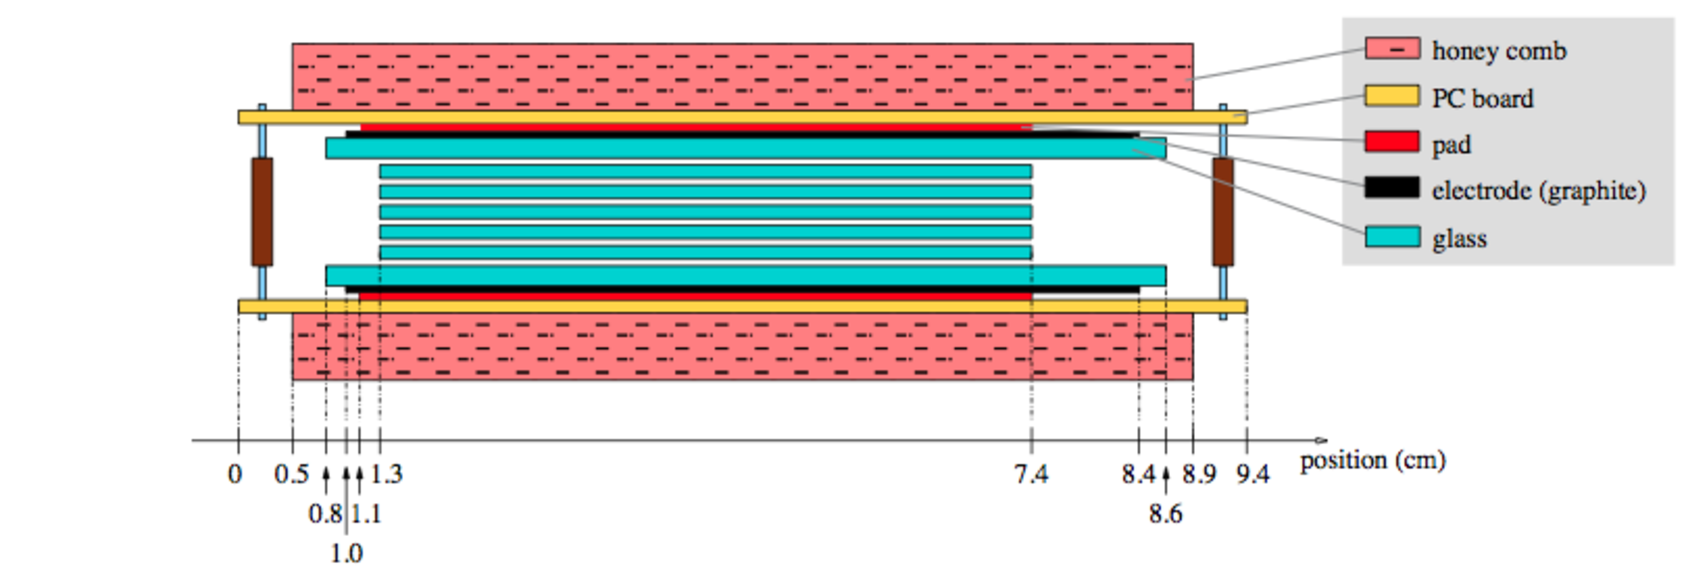
\includegraphics[width = 1\textwidth]{MRPC}
\caption[multi-gap resistive plate chamber]{multi-gap resistive plate chamber (MRPC) used in the TOF detector \cite{largeAreaTOF}}
\label{fig:MRPC}
\end{center}
\end{figure}

The TOF consists of 120 "trays". Each tray, shown in Fig.~ref{fg:starToF}, consists of 32 MRPC modules. The trays are arranged at the outer radius of the TPC, 60 on the east side and 60 on the west. In total they cover two units in pseudorapidity ($-1<\eta<1$), and give full azimuthal coverage. The total time resolution of the TOF system is 87 ps \cite{largeAreaTOF}.   

%The VPD starts the clock for the event and the TOF stops it. The TOF, shown in Fig.~\ref{fig:starToF}, is again a scintillator/PMT detector. It covers about one unit in $\eta$ and about 1/60 of STAR's azimuthal coverage. It is encapsulated in an aluminum tray which is fastened to the outer field cage of the TPC at the 7 o'clock position. There are a total of 41 detector assemblies, each consisting of a 3.81 $\times$ 2 $\times$ 10 cm$^3$ BC420 plastic scintillator and a PMT. The PMTs are specially designed to work inside the STAR magnet.\cite{TOFppVPD}




\begin{figure}
\begin{center}
\includegraphics[width = .9\textwidth]{starToF2}
\caption[STAR Time of Flight System]{One tray of the Time-of-Flight Detector is shown at the 7 o'cock position of STAR. Also shown here are the two VPD detectors on either side of the STAR detector.}
\label{fig:starToF}
\end{center}
\end{figure}

Once the clock is stopped a value of $\beta$ for the track can be calculated as in Eqn.~\ref{eq:tof}. 

\begin{equation}
\label{eq:tof}
\frac{1}{\beta} = \frac{c\tau}{s}
\end{equation}
%
Here $c$ is the speed of light, $\tau$ is the time measured by the time-of-flight system, and $s$ is the path length of the track using the reconstructed path of the TPC. From here the mass of the particle can be found using the momentum of the track measured in the TPC.

\begin{equation}
\label{eq:mtof}
M^2 = \frac{p^2}{\beta^2} - 1
\end{equation}

\begin{figure}
\begin{center}
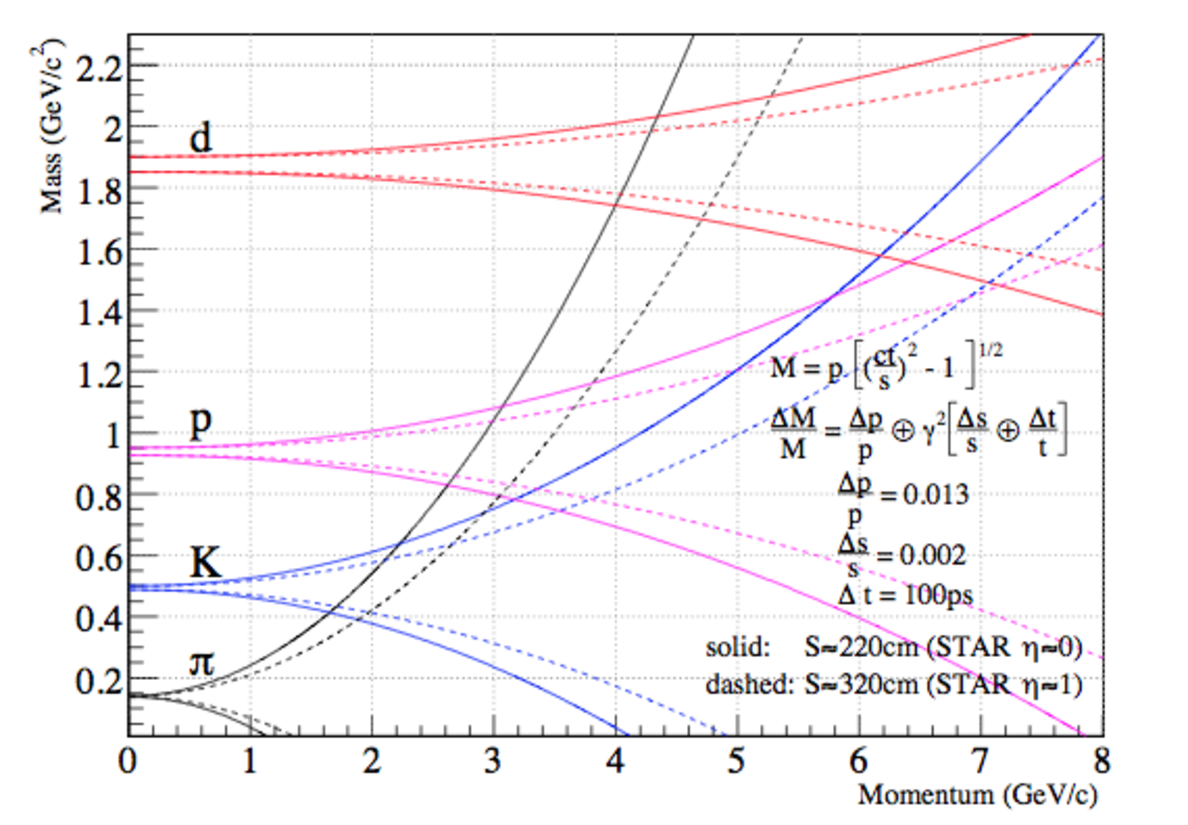
\includegraphics[width = 1\textwidth]{TOFpid}
\caption[Particle identification with TOF]{Particle mass resolution of the STAR TOF system. Solid lines correspond to tracks near $\eta=0$, dashed lines correspond to tracks near $\eta=1$. Particles can be identified with greater than $2\sigma$ confidence in areas where lines do not overlap \cite{largeAreaTOF}.}
\label{fig:tofPID}
\end{center}
\end{figure}



%\section{STAR triggers?}

\chapter{Theoretical Background for Analysis}
\label{ch:theory}

One of the most theoretically clean ways to access the transversity distribution function is through the observation of a single spin asymmetry(SSA) in a semi-inclusive deep inelastic scattering(SIDIS) process between transversely polarized and unpolarized protons where a hadron pair is detected \cite{bacchettaRadici2}. This thesis will be focused mainly on the case where the hadron pair is \pair. At leading twist, only one source for a SSA exists \cite{bacchettaRadici2}. 

The process we are interested in is $p_ap_b^\uparrow \rightarrow \pi^+\pi^- + X$, where unpolarized proton $a$ collides with transversely polarized proton $b$ with spin $\boldsymbol{s}_b$. Outgoing pions with momentum $p_{h,1}$ for the positively charged pion and $p_{h,2}$ for the negatively charged pion are detected. The total pair momentum $\bm{P}_h$ is the sum of $p_{h,1}$ and $p_{h,2}$, the transverse component of which is written as $\ptpair$. 
 The difference of the pion momenta is defined as $\bm{R}= (p_{h,1}-p_{h,2})/2$.

The difference between cross sections when proton $b$ is polarized up and down can be written in a factorized form which includes the transversity distribution $h_1$, and the IFF, $H_1^{\sphericalangle}$.
\begin{align}
\label{eq:crossSecUT}
\text{d}\sigma^\uparrow - \text{d}\sigma^\downarrow = \text{d}\sigma_{UT} = 2\ptpair \sum_{a,b,c,d} |\boldsymbol{s}_b| \frac{|\boldsymbol{R}|}{\mpair}\sin(\phirs) & \int \frac{dx_a dx_b}{8\pi^2 z_c} f_1(x_a) h_1(x_b) \frac{d\Delta\hat{\sigma}_{a b^\uparrow \rightarrow c^\uparrow d}}{d\hat{t}} \nonumber \\ 
&\times \sin\theta H_1^{\sphericalangle c} \left(\bar{z}_c,\cos\theta, {\mpair}^2\right) 
\end{align}
Where $\theta$ is the angle between $p_{h,1}$ in the center of mass frame of the pair and $\bm{P}_h$ in the lab frame. In the above expression, $\phirs = \phis-\phir$, where $\phis$ is the angle between the spin vector of proton $b$ and the scattering plane and $\phir$ is the angle between the scattering plane and the two hadron plane. These angles are shown in Fig.~\ref{fig:angleDeff} and defined as \cite{bacchettaRadici2}
\begin{equation}
\label{eq:angles}
\begin{aligned}[c]
\cos\phi_S &= \frac{(\bm{\hat{P}}_b \times \bm{P}_h)}{|\bm{\hat{P}}_b \times \bm{P}_h|} \cdot \frac{(\bm{\hat{P}}_b \times \bm{S}_b)}{|\bm{\hat{P}}_b \times \bm{S}_b|} \\
\cos\phi_R &= \frac{(\bm{\hat{P}}_h \times \bm{P}_a)}{|\bm{\hat{P}}_h \times \bm{P}_a|} \cdot \frac{(\bm{\hat{P}}_h \times \bm{R})}{|\bm{\hat{P}}_h \times \bm{R}|} \\
\end{aligned}
\qquad
\begin{aligned}[c]
\sin\phi_S &= \frac{(\bm{P}_h \times \bm{S}_b) \cdot \bm{\hat{P}}_b}{|\bm{\hat{P}}_b \times \bm{P}_h| |\bm{\hat{P}}_b \times \bm{S}_b|} \\
\sin\phi_R &= \frac{(\bm{P}_a \times \bm{R}) \cdot \bm{\hat{P}}_h}{|\bm{\hat{P}}_h \times \bm{P}_a| |\bm{\hat{P}}_h \times \bm{R}|} 
\end{aligned}
\end{equation}
where $\bm{P}_a$ and $\bm{P}_b$ are the momenta of protons $a$ and $b$ respectively.

Also appearing in Eqn.~\ref{eq:crossSecUT} is the calculable hard scattering cross section of parton $a$ scattering off of transversly polarized parton $b$ into transversely polarized parton $c$ and parton $d$. Parton $c$ then goes on to fragment into a \pair pair keeping a fraction $z_c$ of parton $c$'s momentum as described by $H_1^{\sphericalangle}$.


%\begin{equation}
%\label{eq:crossSecUT}
%d\sigma_{UT} \propto \ptpair |\overrightarrow{s_a}| \sin(\phirs) \int dx_a dx_b h_1(x_a) f_1(x_b) \frac{d\Delta\hat{\sigma}_{a^\uparrow b \rightarrow c^\uparrow d}}{d\hat{t}}H_1^{\sphericalangle c} \left(z,{\mpair}^2\right) 
%\end{equation}
%\begin{equation}
%\label{eq:crossSecUT_2}
%d\sigma_{UT} = 2\ptpair \sum_{a,b,c,d} |\overrightarrow{s_a}| \sin(\phirs)  \int \frac{dx_a dx_b}{8\pi^2 z_c} h_1(x_a) f_1(x_b) \frac{d\Delta\hat{\sigma}_{a^\uparrow b \rightarrow c^\uparrow d}}{d\hat{t}}\sin\theta H_1^{\sphericalangle c} \left(z_c,\cos\theta, {\mpair}^2\right) 
%\end{equation}

%\begin{align}
%\label{eq:crossSecUT_3}
%d\sigma_{UT} = 2\ptpair \sum_{a,b,c,d} |\boldsymbol{s}_b| \frac{|\boldsymbol{R}|}{\mpair}\sin(\phirs) & \int \frac{dx_a dx_b}{8\pi^2 z_c} f_1(x_a) h_1(x_b) \frac{d\Delta\hat{\sigma}_{a b^\uparrow \rightarrow c^\uparrow d}}{d\hat{t}} \nonumber \\ 
%&\times \sin\theta H_1^{\sphericalangle c} \left(\bar{z}_c,\cos\theta, {\mpair}^2\right) 
%\end{align}
%\begin{align}
%\label{eq:crossSecUT_3}
%d\sigma_{UT} = 2\ptpair \sum_{a,b,c,d} |\overrightarrow{s_a}| \sin(\phirs) & \int \frac{dx_a dx_b}{8\pi^2 z_c} h_1(x_a) f_1(x_b) \frac{d\Delta\hat{\sigma}_{a^\uparrow b \rightarrow c^\uparrow d}}{d\hat{t}} \nonumber \\ 
%&\times \sin\theta H_1^{\sphericalangle c} \left(z_c,\cos\theta, {\mpair}^2\right) 
%\end{align}
%
%Here $|\bm{s}_b|$ is the spin direction of the polarized proton. In our exeriment we always want the polarized proton's spin to be either up or down. However we can't always the it 100\% polarized so we use the polarization of the fill as $|\bm{s}_b|$. Moving on, $\phirs$ is the relative orientation of the outgoing pion pair shown in Fig.~\ref{fig:angleDeff}, $z_c$ is the fraction of the fragmenting quark momentum the pion pair retains, and $\theta$ is the azimuthal angle of the outgoing \pair piar. The difference in momenta of the final state \pair pair is $\boldsymbol{R}$. The hard scattering cross section of a transversely polarized quark $b$ scattering off of an unpolarized quark $a$ into a transversely polarized quark $c$ and an unpolarized quark $d$ $\frac{d\Delta\hat{\sigma}_{a b^\uparrow \rightarrow c^\uparrow d}}{d\hat{t}}$ can be found in Ref.~\cite{bacchettaRadici2}.
%We can make better sense of the above equation by looking closely at each part. First we see the magnitude of the \pair pair transverse momentum. We then see the polarization of the beam. Next is the sinusoidal modulation of the production of \pair pairs. Inside the integral we have the unpolarized distribution function $f_1$, due to the unpolarized  quark $a$ and the transversity distribution function $h_1$ due to the polarized quark $b$. After this we see the elementary scattering cross section of unpolarized quark $a$ scattering off transversely polarized quark $b$ into a transversely polarized quark $c$ and an unpolarized quark $d$. Quark $c$ goes on to fragment into $\pip\pim + X$ described by the IFF $H_1^{\sphericalangle}$, while $d$ goes undetected. 

Comparing this to the cross section when both initial state quarks are unpolarized we see several similarities.
\begin{equation}
\label{eq:crossSecUU}
d\sigma_{UU} = 2 \ptpair \sum_{a,b,c,d} \int \frac{dx_adx_b}{8\pi^2z_c} f_1^a(x_a)f_1^b(x_b) \frac{d\hat{\sigma}_{ab \rightarrow cd}}{d\hat{t}}D_1^c(\bar{z_c},\textnormal{cos}\theta_C,M_C^2)
\end{equation}
As similar as Eqns.~\ref{eq:crossSecUT} and \ref{eq:crossSecUU} look, there are some important differences worth noting. Obviously the polarization isn't there since we now are dealing with unpolarized scattering. The sinusoidal modulation has also disappeared. The transversity distribution has turned into a second unpolarized distribution, and the IFF has turned into $D_1^c$ which is the unpolarized counterpart to the IFF.   

The most important thing to mention is that the sine modulation seen in unpolarized-transversely polarized (U-T) scattering is not seen in unpolarized-unpolarized (U-U) scattering. This means that there is a bias to the yield of \pair pairs in U-T scattering when compared to U-U scattering. We can observe this by looking at the number of \pair pairs at a given value of $\phirs$ when the polarization of the proton beam is $\hat{y}$ $vs$ the number when the polarization is $-\hat{y}$. We then normalize by the number we see at that value of $\phirs$ for U-U scattering, which gives the Single Spin Asymmetry (SSA) $A_{UT}$.
\begin{equation}
\label{eq:asymCS}
A_{UT} \sin (\phirs) =\frac{1}{|\bm{s}_b|} \frac{d\sigma^\uparrow - d\sigma^\downarrow}{d\sigma_{UU}}
\end{equation}

In our experiment we never scatter unpolarized protons, so we have to be clever about the cross section seen in the denominator of Eqn.~\ref{eq:asymCS}. If we sum over the two spin states we are left with the entire unpolarized cross section $d\sigma^\uparrow + d\sigma^\downarrow = d\sigma_{UU}$. Using this, Eqn.~\ref{eq:asymCS} can be rewritten as \cite{bacchettaRadici2, BacchettaThesis, PhysRevLett.80.1166} 
\begin{equation}
\label{eq:SSA}
A_{UT} \sin (\phirs) =\frac{1}{|\bm{s}_b|} \frac{d\sigma^\uparrow - d\sigma^\downarrow}{d\sigma^\uparrow + d\sigma^\downarrow}.
\end{equation}
This is the only source of a single spin asymmetry at leading twist \cite{bacchettaRadici2}. It is important to keep this single spin asymmetry differential in as many kinematic variables as possible, otherwise it is likely to average to zero \cite{keepDifferential}. In this analysis the asymmetry will be kept differential in $\mpair$, $\ptpair$, and $\etapair$ individually. $\etapair$ acts as a surrogate for momentum fraction $x$, as partons with higher $x$ will fragment into hadrons at larger $\eta$. The asymmetry will also be kept differential in two of the three variables simultaneously ($i.e.$, $\mpair$/$\ptpair$, $\mpair$/$\etapair$, and $\ptpair$/$\etapair$). 

Important physics can be seen by performing a partial-wave expansion of the cross section \cite{partialWave}. Expanding $\sin \theta H_1^\sphericalangle$ and looking at the first two terms, 

%\begin{equation}
%\label{eq:partialwaveexpansion}
%\sin \theta H_1^{\sphericalangle c} (\bar{z_c},\cos \theta, {\mpair}^2) \approx H^{\sphericalangle c}_{1,ot}(\bar{z_c},{\mpair}^2) \sin\theta + H^{\sphericalangle c}_{1,lt}(\bar{z_c},{\mpair}^2) \sin\theta \cos\theta
%\end{equation}

\begin{align}
\label{eq:partialwaveexpansion}
\sin \theta H_1^{\sphericalangle c} (\bar{z_c},\cos \theta, {\mpair}^2) \approx &H^{\sphericalangle c}_{1,ot}(\bar{z_c},{\mpair}^2) \sin\theta \nonumber \\
+ &H^{\sphericalangle c}_{1,lt}(\bar{z_c},{\mpair}^2) \sin\theta \cos\theta
\end{align}
%
The first term, S/P wave interference, is due to the interference between amplitudes for a decay into an $L = 0$  \pair pair and an $L = 1$ transversely polarized \pair pair. The second term, P/P wave interference, is due to the interference between amplitudes for a decay into an $L = 1$ \pair pair and an $L = 1$ transversely polarized \pair pair. The $L=1$ contributions comes from a \pair pair that went through a spin-1 intermediate state. One such intermediary we have the ability and statistics to look for is the $\rho$ meson. We expect there to be an enhancement in the IFF, and thus the asymmetry, in the invariant mass region of the $\rho$ (770 MeV) \cite{bacchettaRadici2, Tang}.    



\begin{figure}
\begin{center}
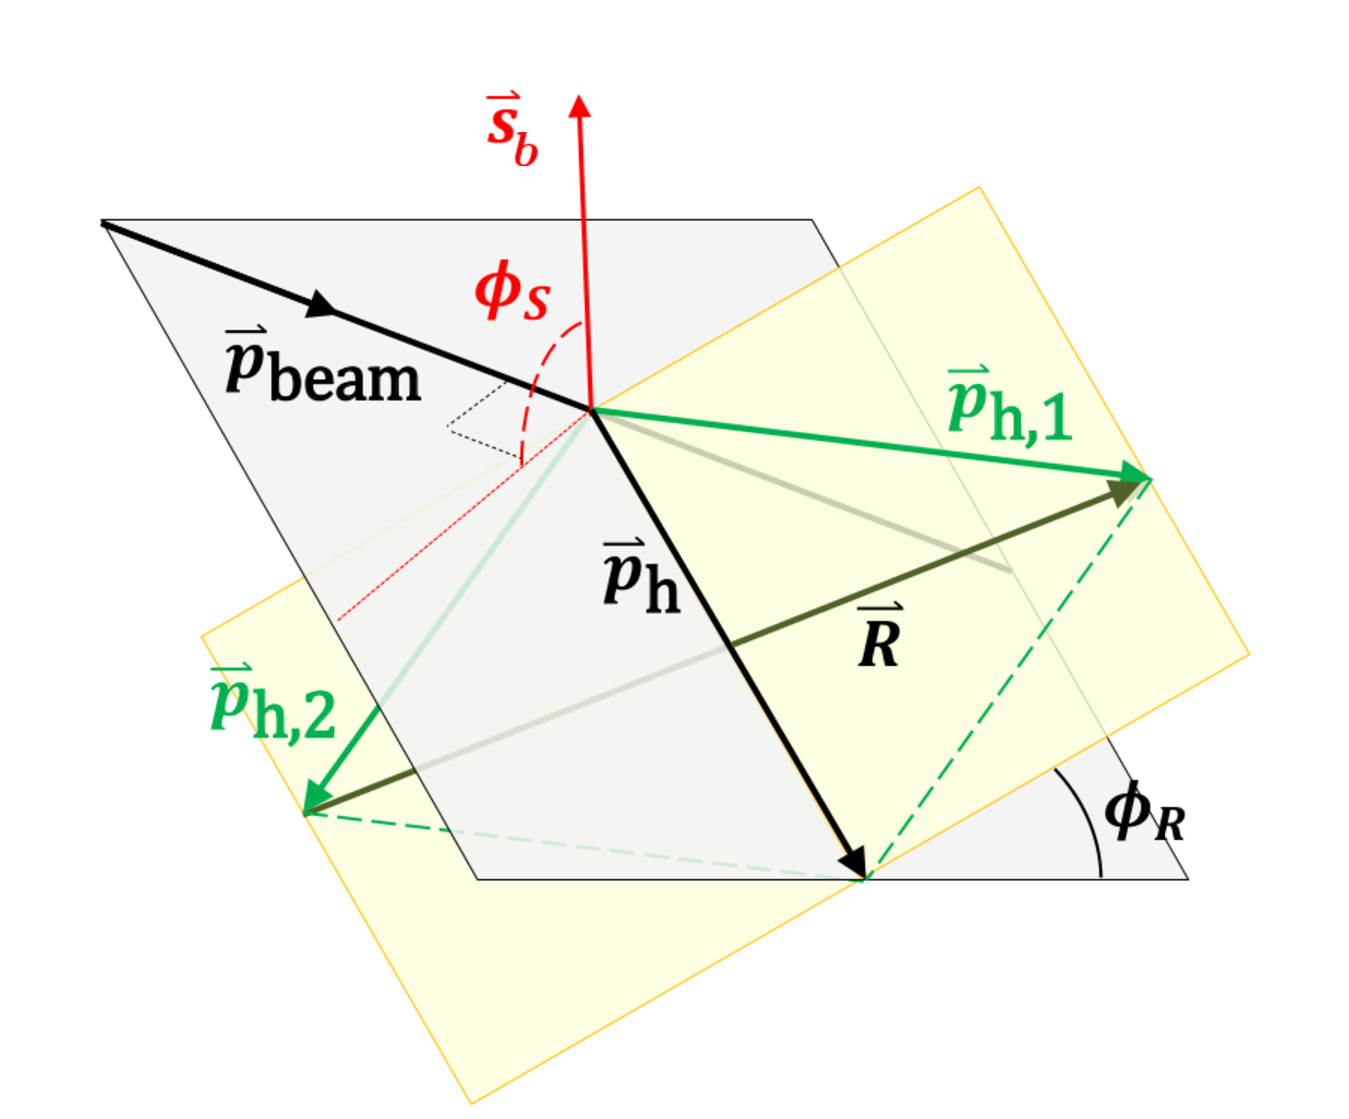
\includegraphics[width = 1\textwidth]{IFF_frame_edit2}
\caption[Angles $\phis$ and $\phir$]{Visual representation of angles $\phi_R$ and $\phi_S$. $\phi_{RS} = \phi_R - \phi_S$ \\ $\vec{p}_{h,1}$ is the momentum of the positive hadron while  $\vec{p}_{h,2}$ is the momentum of the negative hadron.}
\label{fig:angleDeff}
\end{center}
\end{figure}




\chapter{2006 Analysis and Simulation}
\label{chap:2006}

The 2006 data set gave us the first glimpse of this asymmetry in $p+p$ collisions. The analysis of the 2006 data set was done mostly by Dr. Anselm Vossen from Indiana University with an integrated luminosity of 1.8 pb$^{-1}$ of 200 GeV transverse proton proton collisions. The average beam polarization was 60\%~\cite{2006Paper}. 

%Expand this paragraph.  Give a reference for Anselm's work, give the value of the integrated luminosity, etc.


Figure \ref{fig:ansM} shows the asymmetry as a function of the pion pair invariant mass. As hinted from the theory there is an increase in the asymmetry around the $\rho$ meson mass for both forward ($\eta > 0$) and backward pairs ($\eta < 0$). 


 \begin{figure}
\begin{center}
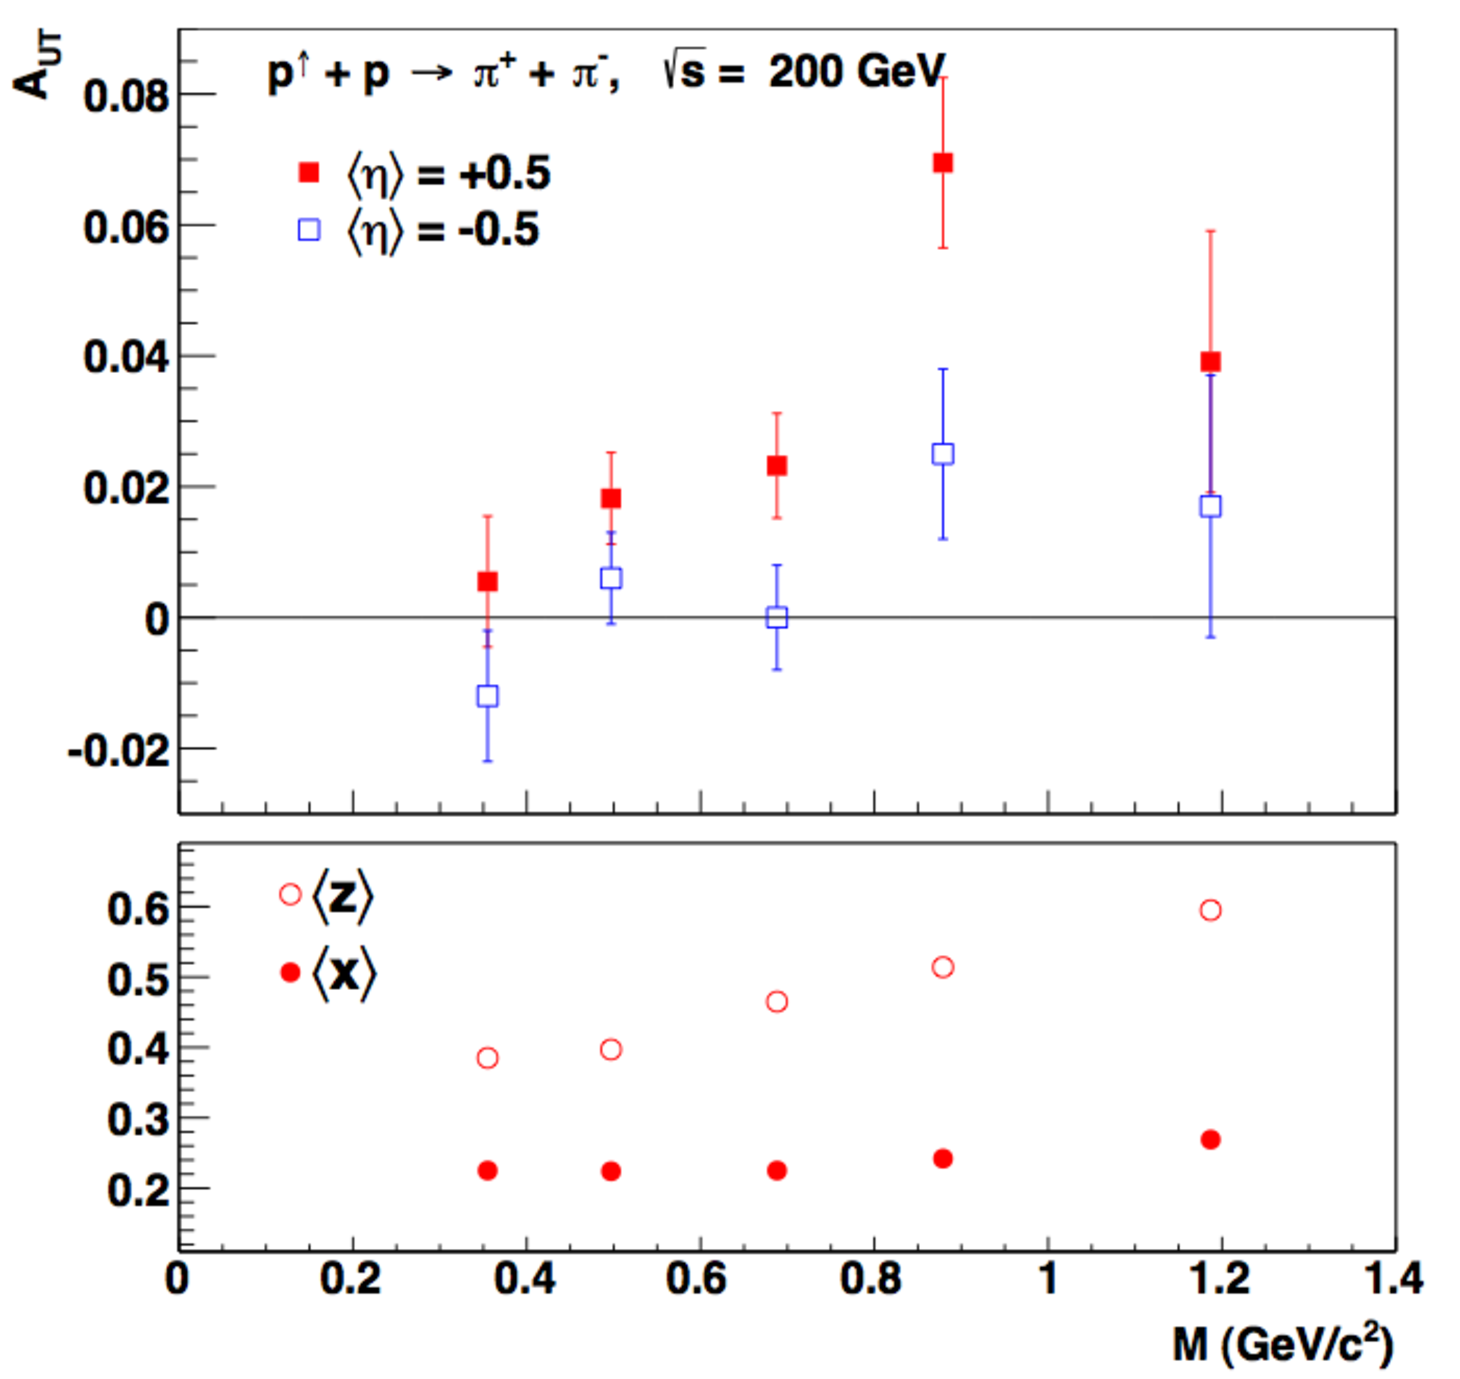
\includegraphics[width = 1\textwidth]{ansM_new}
\caption[$A_{UT}$ $vs$ Invariant Mass in the 2006 data set]{Asymmetry versus invariant mass of the \pair pair for the 2006 data set for pairs scattering in the forward direction (red) and in the backward direction (blue).}
\label{fig:ansM}
\end{center}
\end{figure}


Varying the opening angle of the pion pair addresses the $z$ dependence of the asymmetry. The fraction of the fragmenting quark momentum the pion pair retains, $z$, influences the size of the IFF. It turns out the asymmetry increases as the opening angle decreases as seen in Fig.~\ref{fig:ansAng}.

 \begin{figure}
\begin{center}
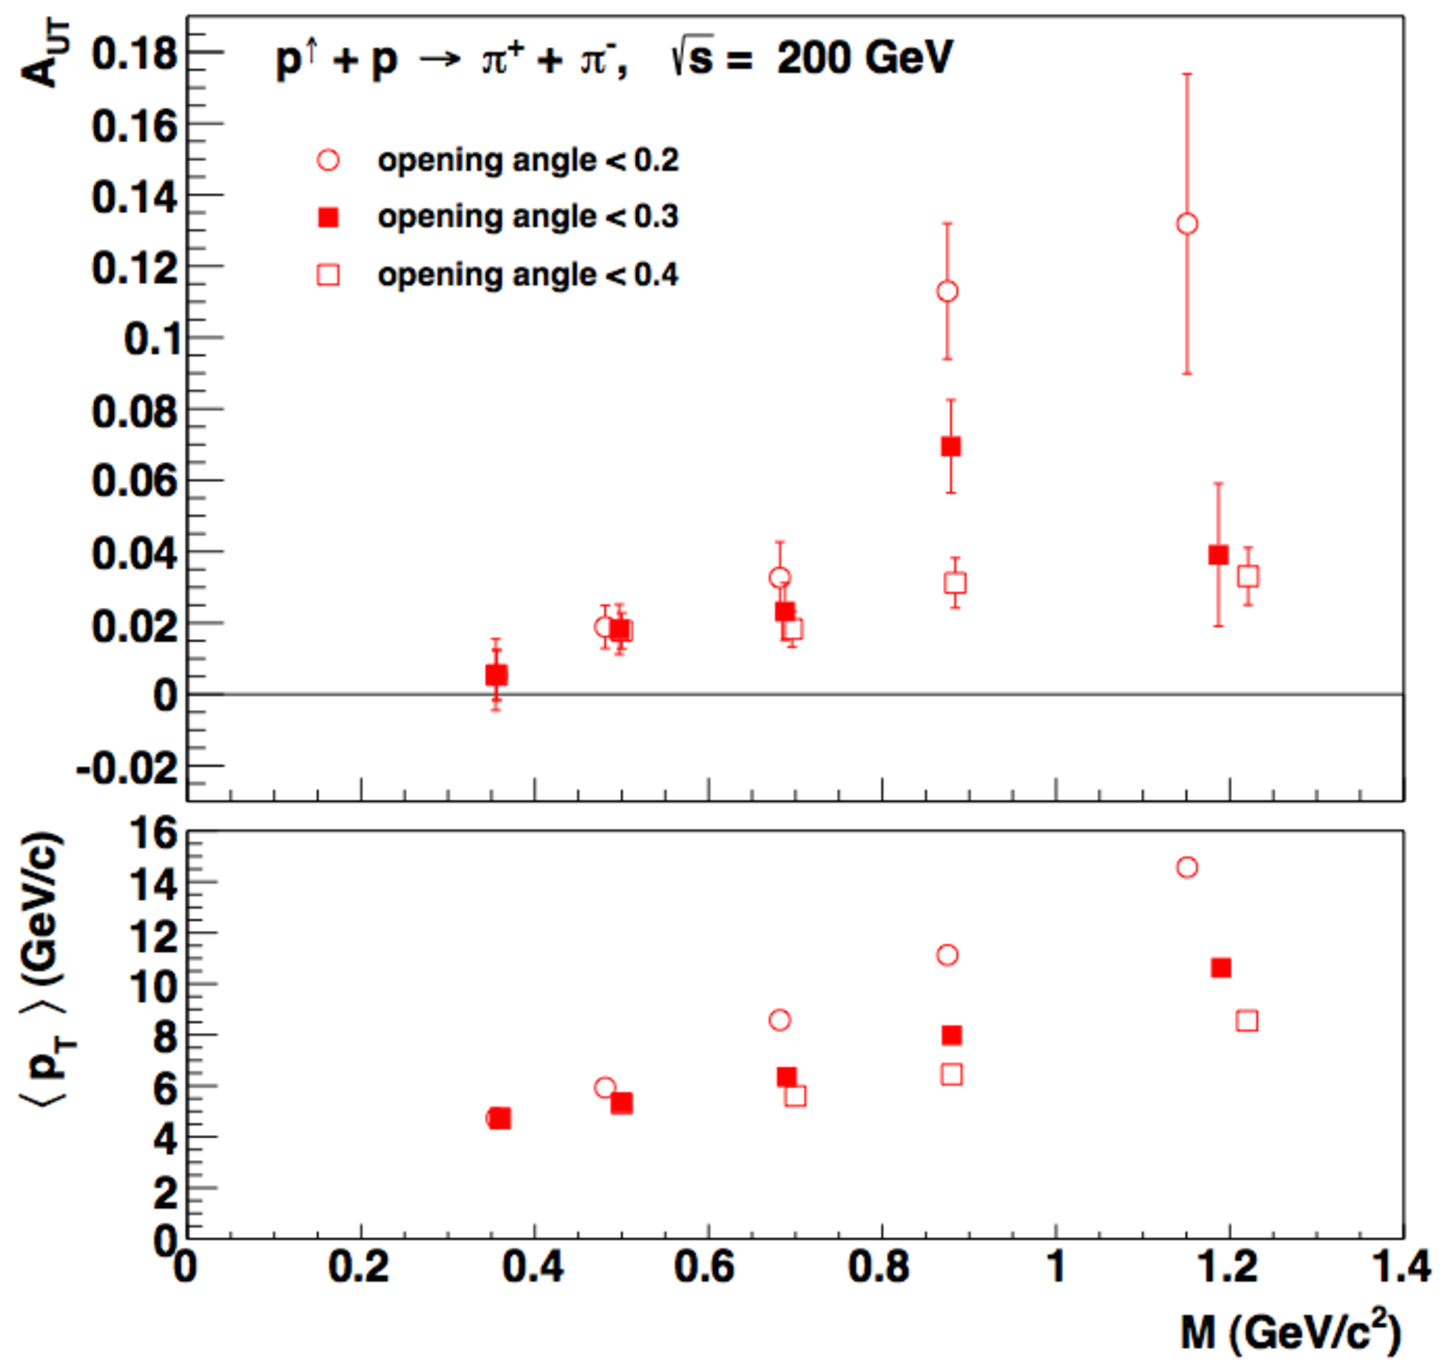
\includegraphics[width = 1\textwidth]{ansAngles_new}
\caption[$A_{UT}$ for different opening angles]{Asymmetry versus invariant mass of the \pair pair for the 2006 data set for different opening angles of pairs are scattered into the forward direction.}
\label{fig:ansAng}
\end{center}
\end{figure}

As stated previously, $\etapair$ acts as a surrogate for the momentum fraction of the polarized parton, as a larger partonic momentum fraction will cause the pion pair to be produced in a more forward direction. The asymmetry is plotted as a function of $\etapair$ in Fig.~\ref{fig:ansEta}. As one might expect, the asymmetry is larger the more forward the pion pair is. This is explained by the fact that pairs from more forward pseudorapidity result from polarized partons with larger momentum fractions, allowing for a larger spin transfer. 

A supplemental analysis was done on simulated data to investigate partonic momentum fractions as well as biases introduced by STAR triggers. Figure \ref{fig:2006SimX} shows the momentum fraction of the fragmenting quark for pairs in the forward and reverse directions. This bias toward higher $x$ events is shown in Fig.~\ref{fig:TriggerBiasXHiQualColor}. A more in-depth discussion about the need for an analysis on simulated data as well as the results of the analysis on the 2012 simulation is given in appendix \ref{ch:trigBias}.

 \begin{figure}
\begin{center}
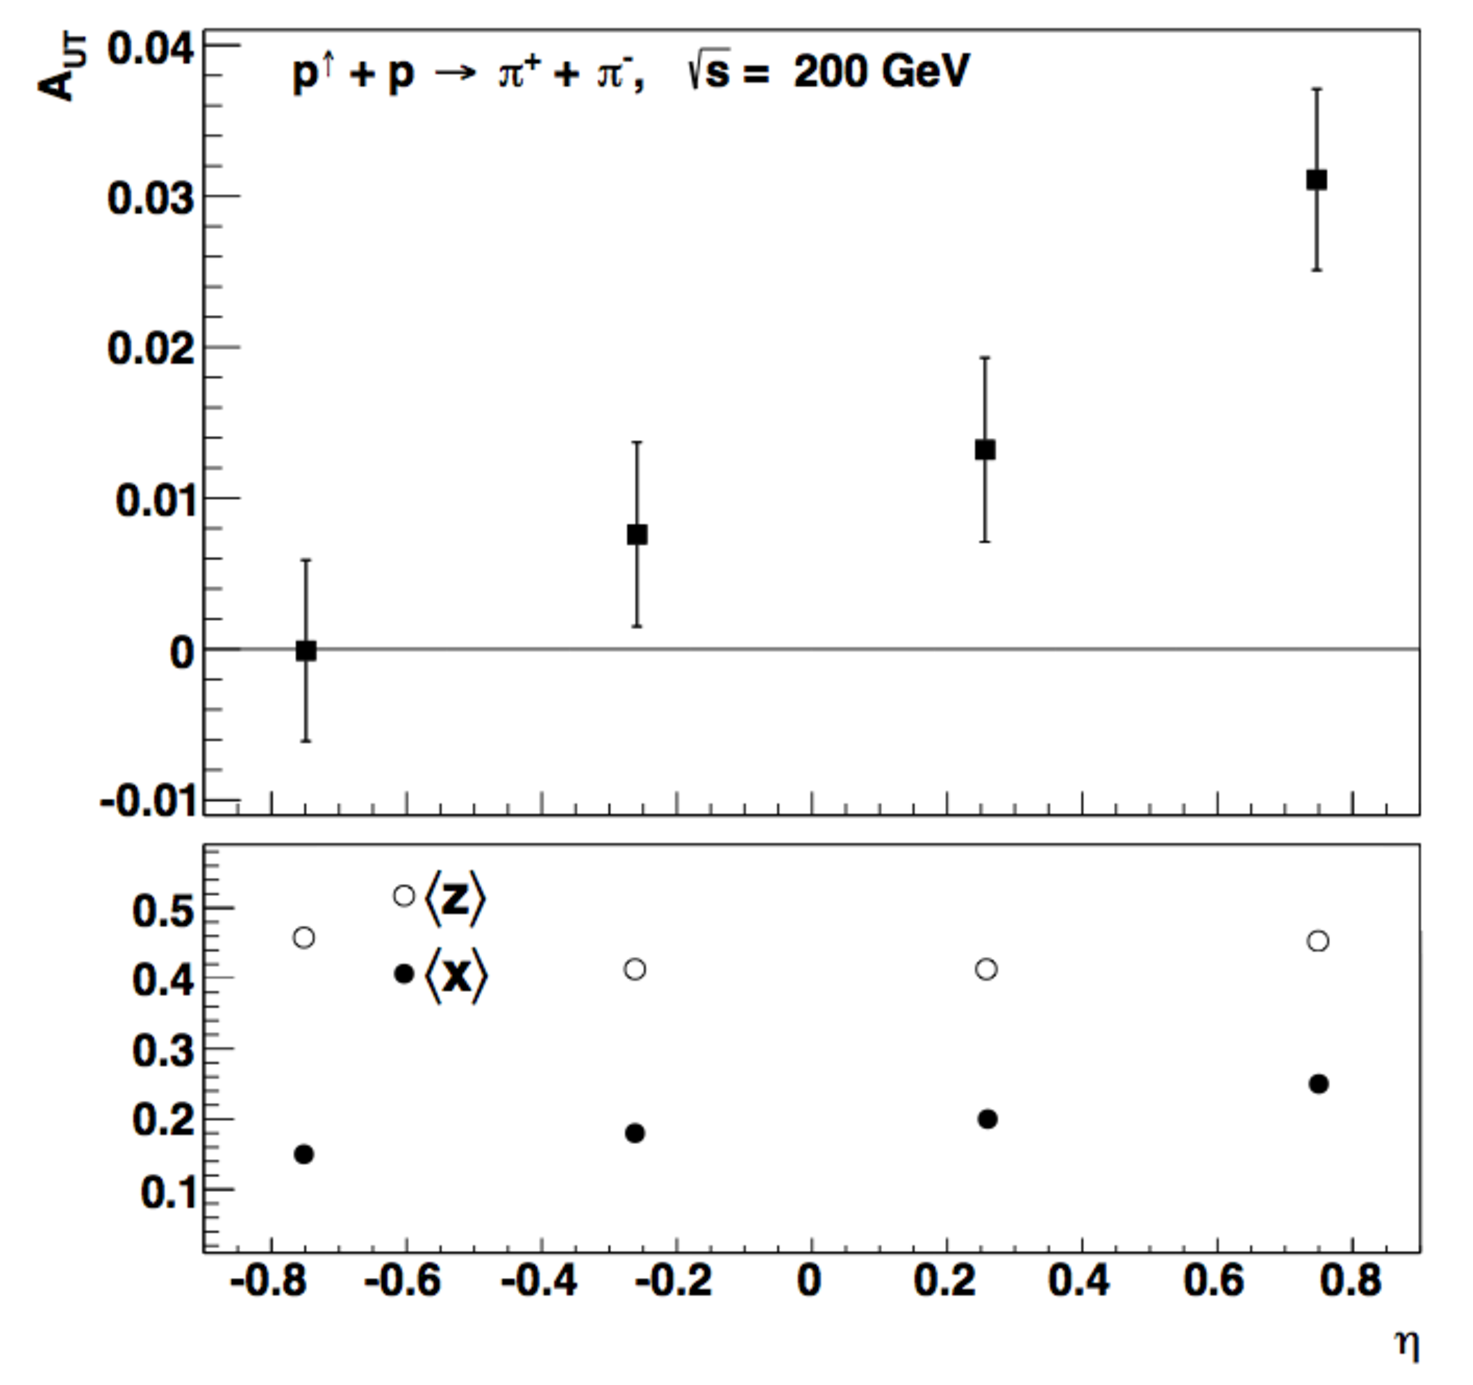
\includegraphics[width = 1\textwidth]{ansEta_new}
\caption[$A_{UT}$ vs $\etapair$ in 2006 data set]{Asymmetry versus $\etapair$ for the 2006 data set}
\label{fig:ansEta}
\end{center}
\end{figure}

 \begin{figure}
\begin{center}
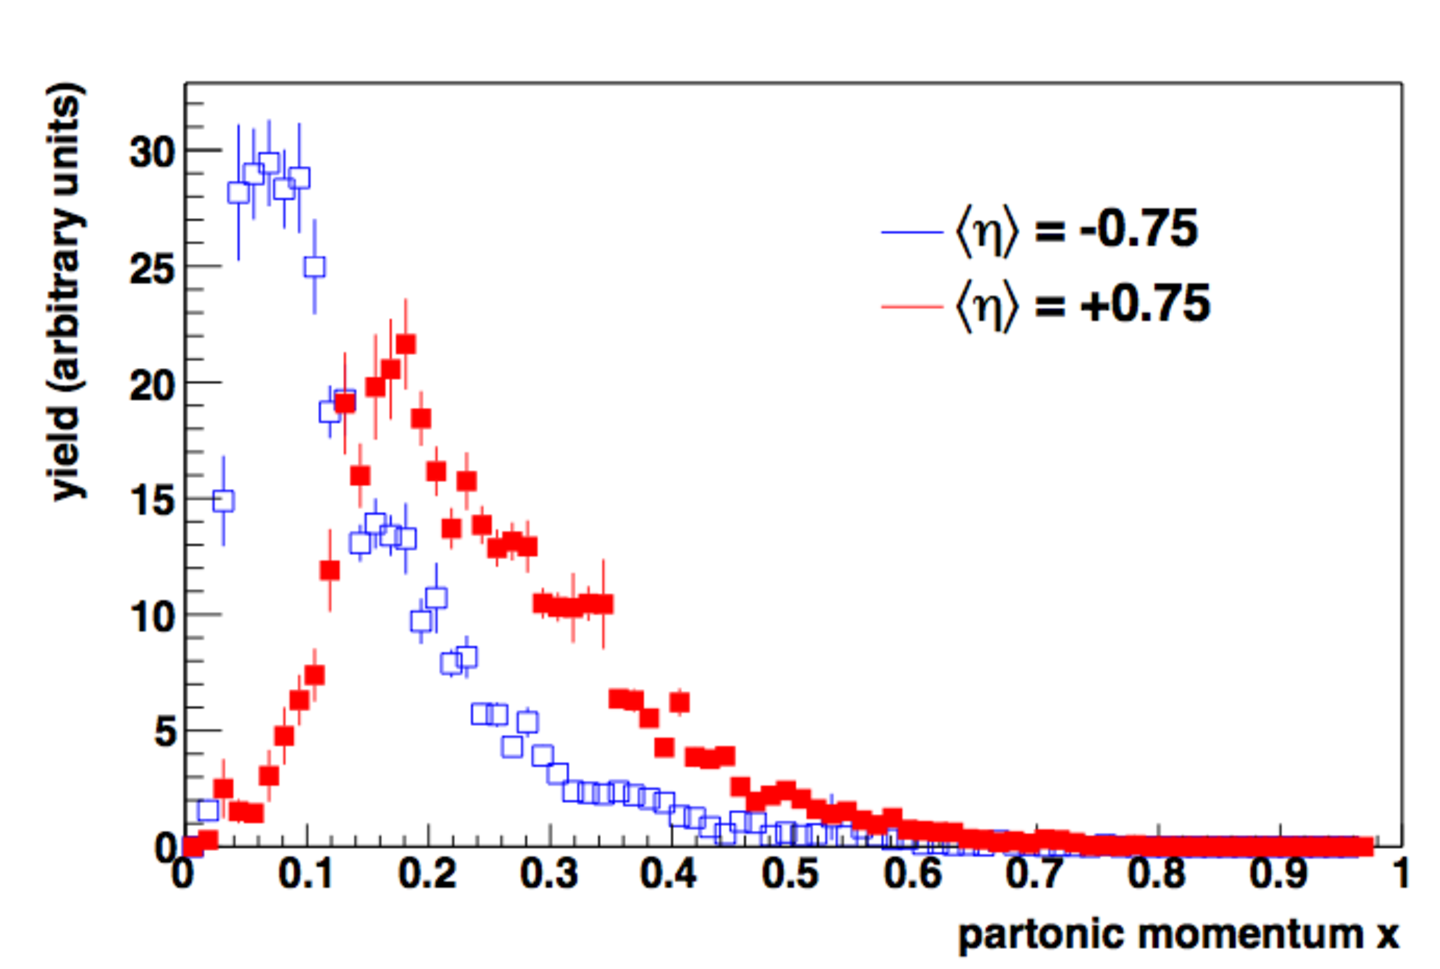
\includegraphics[width = 1\textwidth]{2006SimX}
\caption[Partonic momentum fraction in 2006 simulation forward and backward \pair pair]{Partonic momentum fraction $x$ obtained from simulation for the parton from the polarized proton in the forward (red) and backward (blue) direction}
\label{fig:2006SimX}
\end{center}
\end{figure}

\begin{figure}
\begin{center}
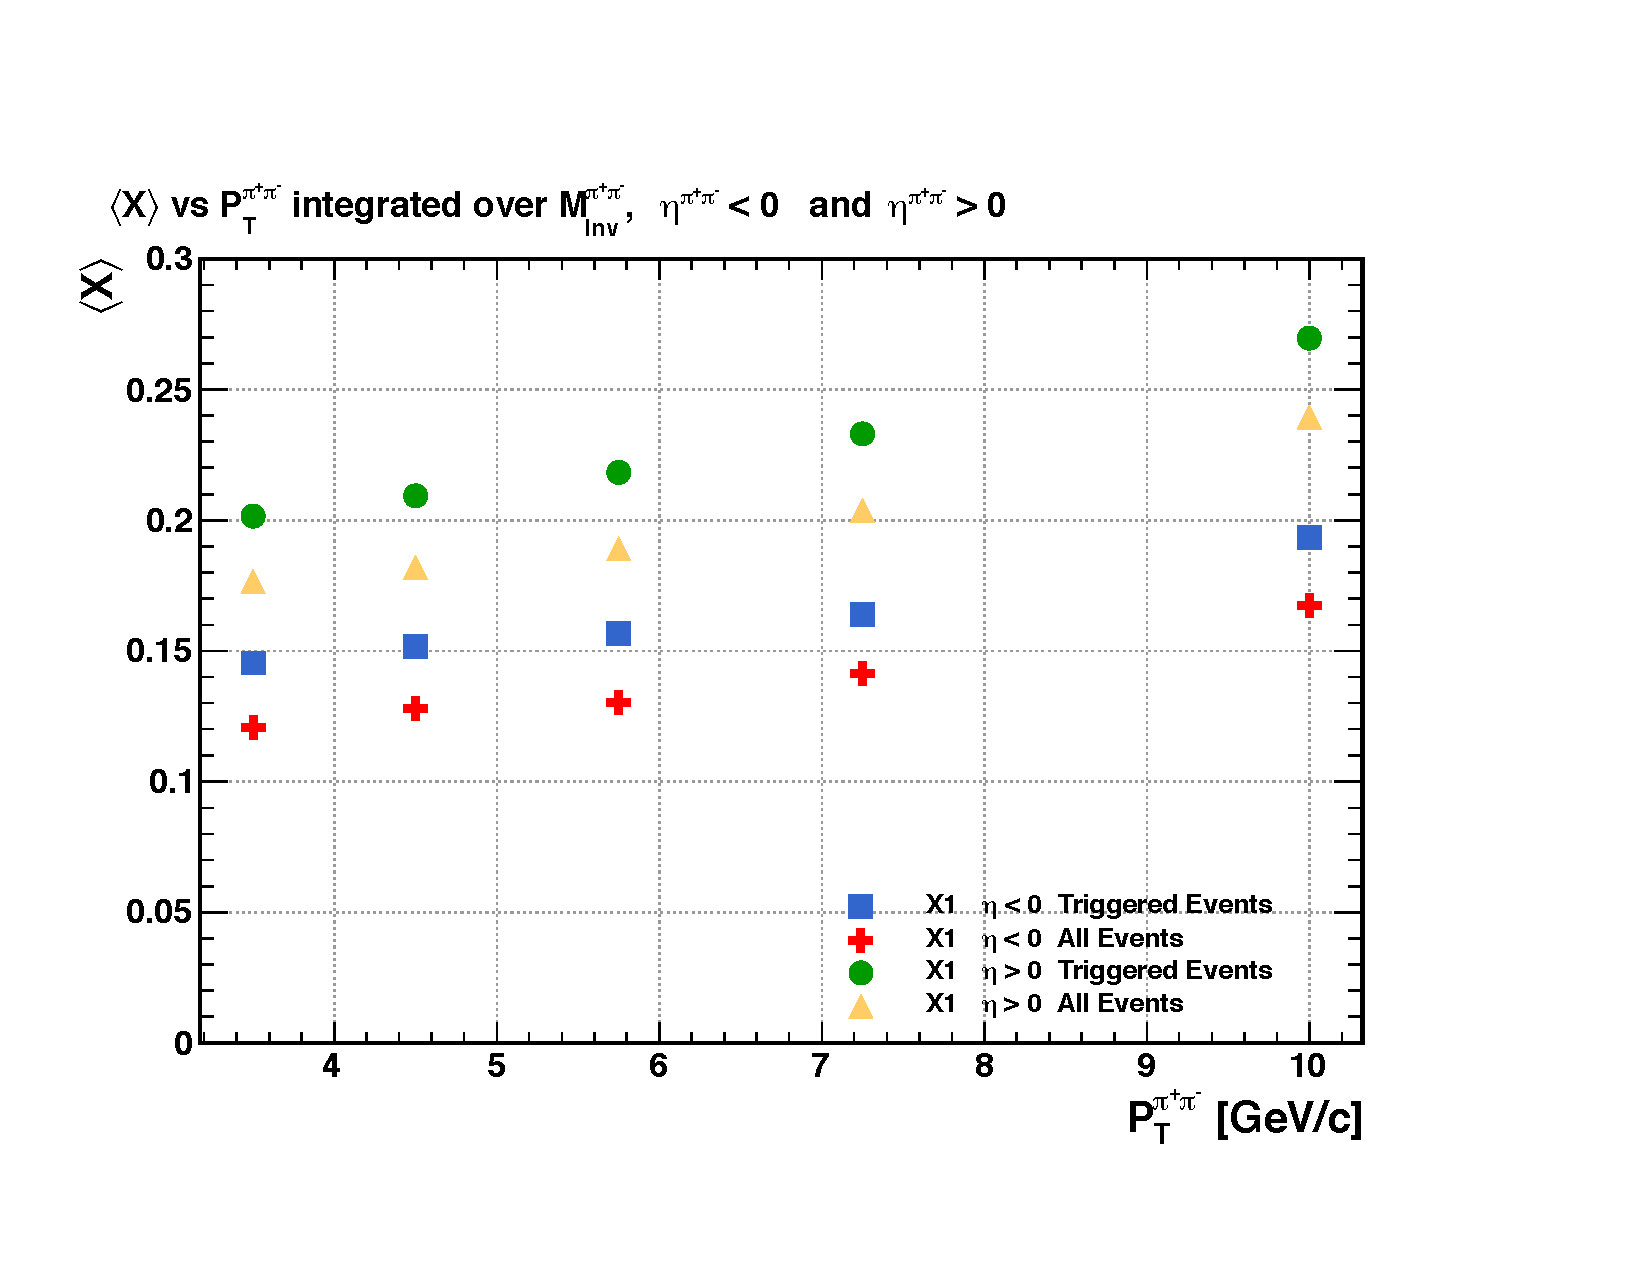
\includegraphics[width = 1\textwidth]{TriggerBiasXHiQualColor}
\caption[Trigger bias toward higher momentum fraction $x$ events]{The averge momentum fraction $x$ of the polarized quark (quark 1) is larger for triggered events than for all events. This effefct is seen in both the forward and backward directions and for all \pair transverse momenta. Note: this figure is caclulated for the 2006 detector configuration and triggers.}
\label{fig:TriggerBiasXHiQualColor}
\end{center}
\end{figure}



These results are the first sign of non-zero asymmetries in \pair pair correlation in polarized proton collisions. More can be read about the 2006 study in reference \cite{2006Paper}.

\chapter{2012 IFF}

\section{Data Set, Triggers, and Cuts}

The total integrated luminosity for the 2012 200GeV transverse proton data set was 7.74 pb$^-1$ \cite{BeamUse}. The runs from the 2012 production that passed quality tests and are eligible to be used in the analysis are listed in the table below. The average beam polarization from pairs found in these runs is 61.618 $\pm .003 \%$.
%\begin{center}
%\begin{table}[h!]
\tiny{
\begin{longtable}{cccccccc} \hline
13044126  &  13045001  &  13045003  &  13045005  &  13045006  &  13045007  &  13045012  &  13045029  \\ 
13045056  &  13045133  &  13045134  &  13045135  &  13045138  &  13045145  &  13045146  &  13045164  \\ 
13046001  &  13046002  &  13046003  &  13046004  &  13046011  &  13046012  &  13046013  &  13046014  \\ 
13046015  &  13046017  &  13046121  &  13047003  &  13047004  &  13047022  &  13047023  &  13047024  \\ 
13047026  &  13047027  &  13047028  &  13047029  &  13047030  &  13047031  &  13047032  &  13047033  \\ 
13047034  &  13047035  &  13048010  &  13048011  &  13048012  &  13048013  &  13048014  &  13048015  \\ 
13048016  &  13048017  &  13048018  &  13048019  &  13048030  &  13048031  &  13048032  &  13048040  \\ 
13048041  &  13048042  &  13048043  &  13048044  &  13048045  &  13048046  &  13048049  &  13048050  \\ 
13048051  &  13048052  &  13048053  &  13048087  &  13048088  &  13048089  &  13048090  &  13048091  \\ 
13048092  &  13048093  &  13049031  &  13049032  &  13049035  &  13049039  &  13049041  &  13049042  \\ 
13049044  &  13049045  &  13049046  &  13049047  &  13049048  &  13049049  &  13049050  &  13049072  \\ 
13049073  &  13049080  &  13049081  &  13049082  &  13049089  &  13049093  &  13049094  &  13049096  \\ 
13049098  &  13049099  &  13049101  &  13050001  &  13050007  &  13050009  &  13050011  &  13050012  \\ 
13050015  &  13050016  &  13050020  &  13050022  &  13050023  &  13050028  &  13050029  &  13050031  \\ 
13050032  &  13050033  &  13050036  &  13050037  &  13050038  &  13050039  &  13050041  &  13050043  \\ 
13050044  &  13050046  &  13050047  &  13050049  &  13050050  &  13051011  &  13051012  &  13051015  \\ 
13051016  &  13051017  &  13051019  &  13051020  &  13051021  &  13051022  &  13051023  &  13051024  \\ 
13051026  &  13051028  &  13051074  &  13051080  &  13051081  &  13051083  &  13051085  &  13051086  \\ 
13051087  &  13051088  &  13051092  &  13051093  &  13051095  &  13052001  &  13052002  &  13052003  \\ 
13052004  &  13052005  &  13052009  &  13052010  &  13052011  &  13052012  &  13052013  &  13052014  \\ 
13052015  &  13052016  &  13052017  &  13052018  &  13052020  &  13052021  &  13052022  &  13052037  \\ 
13052039  &  13052042  &  13052043  &  13052045  &  13052048  &  13052050  &  13052051  &  13052052  \\ 
13052053  &  13052054  &  13052056  &  13052088  &  13053004  &  13053005  &  13053006  &  13053007  \\ 
13053012  &  13053013  &  13053015  &  13053027  &  13053028  &  13054022  &  13054023  &  13054044  \\ 
13054045  &  13054060  &  13054061  &  13054062  &  13054063  &  13054064  &  13054065  &  13054066  \\ 
13054068  &  13054069  &  13054084  &  13054085  &  13055004  &  13055006  &  13055007  &  13055008  \\ 
13055009  &  13055010  &  13055011  &  13055014  &  13055016  &  13055017  &  13055018  &  13055019  \\ 
13055020  &  13055021  &  13055022  &  13055023  &  13055024  &  13055035  &  13055036  &  13055037  \\ 
13055038  &  13055039  &  13055068  &  13055070  &  13055072  &  13055075  &  13055076  &  13055080  \\ 
13055081  &  13055082  &  13055086  &  13055087  &  13056005  &  13056007  &  13056008  &  13056020  \\ 
13056021  &  13056022  &  13056023  &  13056024  &  13056025  &  13056026  &  13056027  &  13056028  \\ 
13056029  &  13056030  &  13056031  &  13056033  &  13056034  &  13056035  &  13056037  &  13056038  \\ 
13056039  &  13057011  &  13057014  &  13057015  &  13057016  &  13057017  &  13057018  &  13057019  \\ 
13057021  &  13057022  &  13057023  &  13057024  &  13057025  &  13057026  &  13057027  &  13057044  \\ 
13057045  &  13057046  &  13057047  &  13057048  &  13057049  &  13057050  &  13057051  &  13057052  \\ 
13057053  &  13057055  &  13057056  &  13057057  &  13057058  &  13058002  &  13058015  &  13058016  \\ 
13058017  &  13058018  &  13058025  &  13058026  &  13058028  &  13058029  &  13058030  &  13058031  \\ 
13059084  &  13060010  &  13061024  &  13061025  &  13061026  &  13061030  &  13061031  &  13061035  \\ 
13061054  &  13061055  &  13061059  &  13061060  &  13061061  &  13062001  &  13062002  &  13062004  \\ 
13062005  &  13062006  &  13062007  &  13062013  &  13062025  &  13062026  &  13062028  &  13062029  \\ 
13062049  &  13062050  &  13062052  &  13062059  &  13062060  &  13062061  &  13062062  &  13062063  \\ 
13063009  &  13063010  &  13063011  &  13063020  &  13063022  &  13063023  &  13063030  &  13063031  \\ 
13063032  &  13063033  &  13063034  &  13063035  &  13063036  &  13063053  &  13063054  &  13063062  \\ 
13063063  &  13063065  &  13063067  &  13063068  &  13063071  &  13063072  &  13063073  &  13063074  \\ 
13063076  &  13064001  &  13064002  &  13064003  &  13064004  &  13064005  &  13064006  &  13064012  \\ 
13064014  &  13064020  &  13064021  &  13064022  &  13064023  &  13064024  &  13064025  &  13064026  \\ 
13064028  &  13064029  &  13064030  &  13064031  &  13064032  &  13064052  &  13064055  &  13064056  \\ 
13064057  &  13064059  &  13064061  &  13064064  &  13064065  &  13064066  &  13064068  &  13064070  \\ 
13064074  &  13064075  &  13065005  &  13065006  &  13065007  &  13065008  &  13065009  &  13065013  \\ 
13065014  &  13065015  &  13065016  &  13065017  &  13065018  &  13065019  &  13065020  &  13065021  \\ 
13065022  &  13065047  &  13065048  &  13065049  &  13065050  &  13065052  &  13065053  &  13065055  \\ 
13065056  &  13065058  &  13065059  &  13065060  &  13066021  &  13066022  &  13066023  &  13066024  \\ 
13066025  &  13066026  &  13066027  &  13066028  &  13066029  &  13066030  &  13066031  &  13066033  \\ 
13066034  &  13066035  &  13066036  &  13068084  &  13068088  &  13068090  &  13069001  &  13069002  \\ 
13069003  &  13069004  &  13069005  &  13069006  &  13069007  &  13069014  &  13069016  &  13069017  \\ 
13069018  &  13069020  &  13069021  &  13069022  &  13069023  &  13069024  &  13069026  &  13069027  \\ 
13069029  &  13069030  &  13069031  &  13069035  &  13069036  &  13069066  &  13069067  &  13069068  \\ 
13069069  &  13069073  &  13070006  &  13070008  &  13070010  &  13070011  &  13070012  &  13070014  \\ 
13070015  &  13070016  &  13070017  &  13070018  &  13070019  &  13070020  &  13070021  &  13070022  \\ 
13070024  &  13070025  &  13070026  &  13070027  &  13071009  &  13071010  &  13071011  &  13071012  \\ 
13072006  &  13072014  &  13072015  &  13072016  &  13072017  &  13072018  &  13072019  &  13072020  \\ \hline
\end{longtable}
} 
\normalsize

From these runs, events were selected which triggered at least one of the following STAR triggers of interest: JP0, JP1, JP2, AJP, BHT0VPD, BHT1VPD, BHT2BBC, or BHT2. These were chosen because they were most similar to the triggers used to select events in the 2006 analysis, thus allowing for a proper comparison of the results. The thresholds for these triggers can be found in table \ref{tab:thresh}.

\begin{table}[h!]
\begin{center}
\begin{tabular}{|c|c|} \hline
Trigger & Threshold  \\
\hline
BEMC-JP0	& 20  \\
BEMC-JP1	& 28  \\
BEMC-JP2	& 36  \\
BEMC-HT0	& 11  \\
BEMC-HT1	& 15  \\
BEMC-HT2	& 18  \\
VPD-TACdiff-MAX	& 4083  \\
VPD-TACdiff-MIN	&  3883 \\
VPD-East-ADC-SUM & 10 \\
VPD-West-ADC-SUM & 10 \\
BBC-Small-TACdiff-MAX	& 4933  \\
BBC-Small-TACdiff-MIN	& 3267  \\
BBC-Small-East-ADC-SUM	& 20  \\
BBC-Small-West-ADC-SUM	& 20  \\
\hline
\end{tabular}
\caption{Relevant Trigger Thresholds}
\label{tab:thresh}
\end{center}
\end{table}


%needs an estimate of the integrated luminosity and luminosity weighted polarization for each beam (with errors).
% you also need a description of what each trigger was, eg.
% JP sums tower energies in a patch Del_etaxDel_phi ~1x1.
% Different energy thresholds. prescales for lower threshold
% triggers.
% you also need a distribution of the Z vertex distribution.

Tracks from these triggered events were then scrutinized. As the BEMC only covers a finite range in $\eta$, tracks at pseudorapidity greater than $2$ and less than $-2$ were rejected. To ensure good track resolution in the TPC necessary for particle identification, tracks with less than five fit points were also rejected. Since different trajectories in the TPC offer a different number of possible fit points, tracks are also required to have at least half of the possible fit points. The position of the vertex the track originated is required to be less than 60 cm from the center of the STAR detector. This helps the detector reconstruct the correct kinematic location of the particle. The track is also required to have a transverse momentum larger than 1.5 $GeV/c$. If a track possesses all the required attributes, it is included in the analysis.


\section{Particle Identification and Contamination}

Once a track is selected for the analysis, identification of the particle type is an important next step. As charged particles traverse the TPC, they lose energy when ionizing the TPC gas. This specific energy loss is a function of velocity, and is therefore different for different particles at a given momentum. A value, $n_\sigma(\pi)$, is given to each track in an event describing how many standard deviations away it's energy loss is from the expected energy loss for a pion on the ionization energy loss curve shown in Fig.~\ref{fig:tpcDedx2}; the ideal curves showing the expected energy loss for each species are given as black lines. Each track is also given values of $n_\sigma(p)$, $n_\sigma(k)$, and $n_\sigma(e)$ describing how close they are to ideal protons, kaons, and electrons. For example if a track has an $n_\sigma(\pi)$ value of zero and a momentum at which the ideal energy loss curves don't intersect, it is very likely a pion and should be included in the analysis. 

 \begin{figure}
\begin{center}
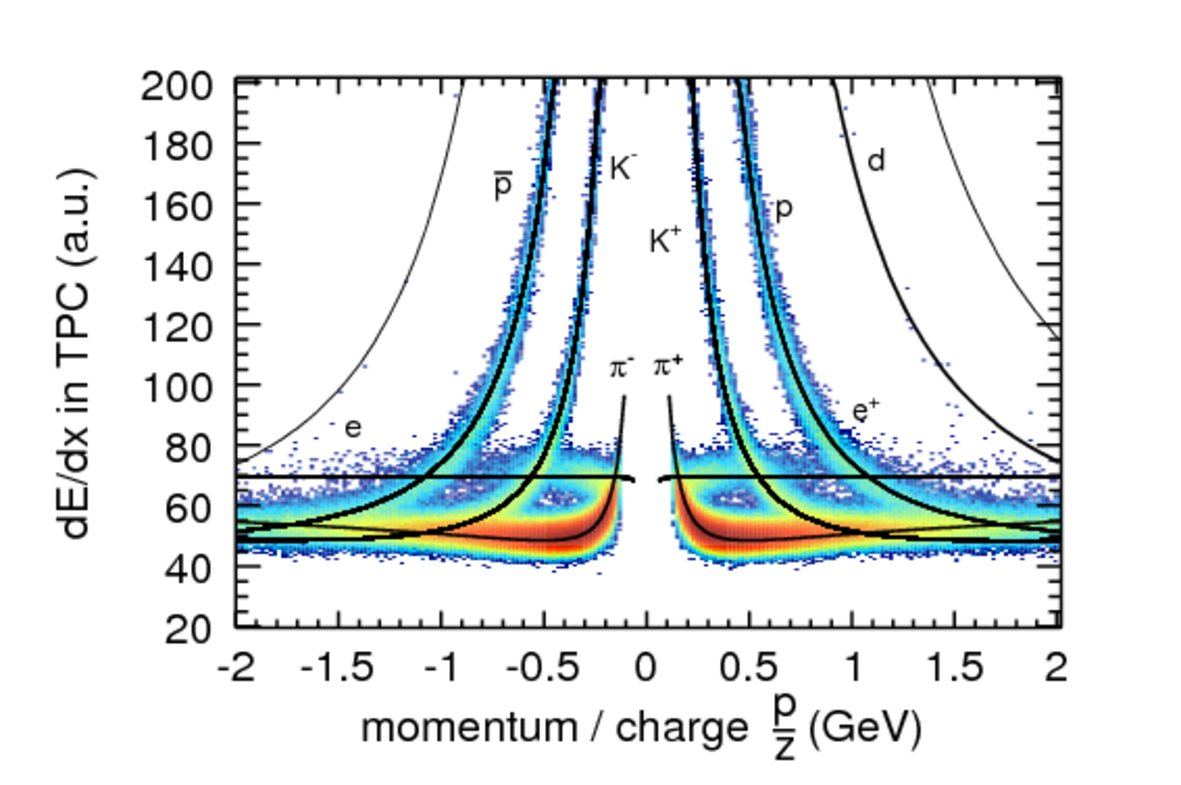
\includegraphics[width = .8\textwidth]{TPC_dedx2}
\caption[Ionization energy loss in TPC]{Ionization energy loss as a function of particle momentum divided by electric charge for TPC tracks}
\label{fig:tpcDedx2}
\end{center}
\end{figure}


If the data set strictly contained pions, the $n_\sigma(\pi)$ distribution would be gaussian centered around zero. However as seen in Fig.~\ref{fig:nSigExample} it is not exactly gaussian. Although it looks gaussian near $n_\sigma(\pi) = 0$, there is a clear shoulder on the left side due to kaon and proton contamination and a smaller shoulder to the right from electron contamination. To account for this contamination, we fit the $n_\sigma(\pi)$ distribution with a 5-gaussian fit; one gaussian for each particle species plus one gaussian to account for the tail at high $n_\sigma(\pi)$ most likely due to pile up or merged tracks. 

Several of the degrees of freedom of the fit can be constrained for physical reasons. First, the expected $n_\sigma(\pi)$ value of an ideal kaon can be readily found from fitting a plot of $n_\sigma(\pi)$ vs $n_\sigma(k)$ as in Fig.~\ref{fig:nSignSig}. The separation between the pion and kaon gaussians in the 5-gaussian fit is required to be equal to the value of $n_\sigma(\pi)$ at $n_\sigma(k) = 0$. This is repeated to constrain the separation between the pion and proton gaussians, as well as the separation between the pion and electron gaussians. Secondly, kaons and protons are required to have the same width. Third the ``pile up" gaussian is required to have a smaller amplitude and be located at a larger $n_\sigma(\pi)$ than the electron gaussian. This is to make sure it actually does fit the high $n_\sigma(\pi)$ tail. This tail is more prominent at higher track momentum but is sometimes absent at lower momentum.  

Armed with this fitting procedure, the location and amount of each particle species becomes clear (Fig.~\ref{fig:nSigExampleFit}). A clean sample of pions can be found by selecting tracks with an $n_\sigma(\pi)$ between $-1$ and 2.5. This choice maximizes the number of pions included in the analysis while not compromising the purity of the pion sample too much.  


         
 \begin{figure}
\begin{center}
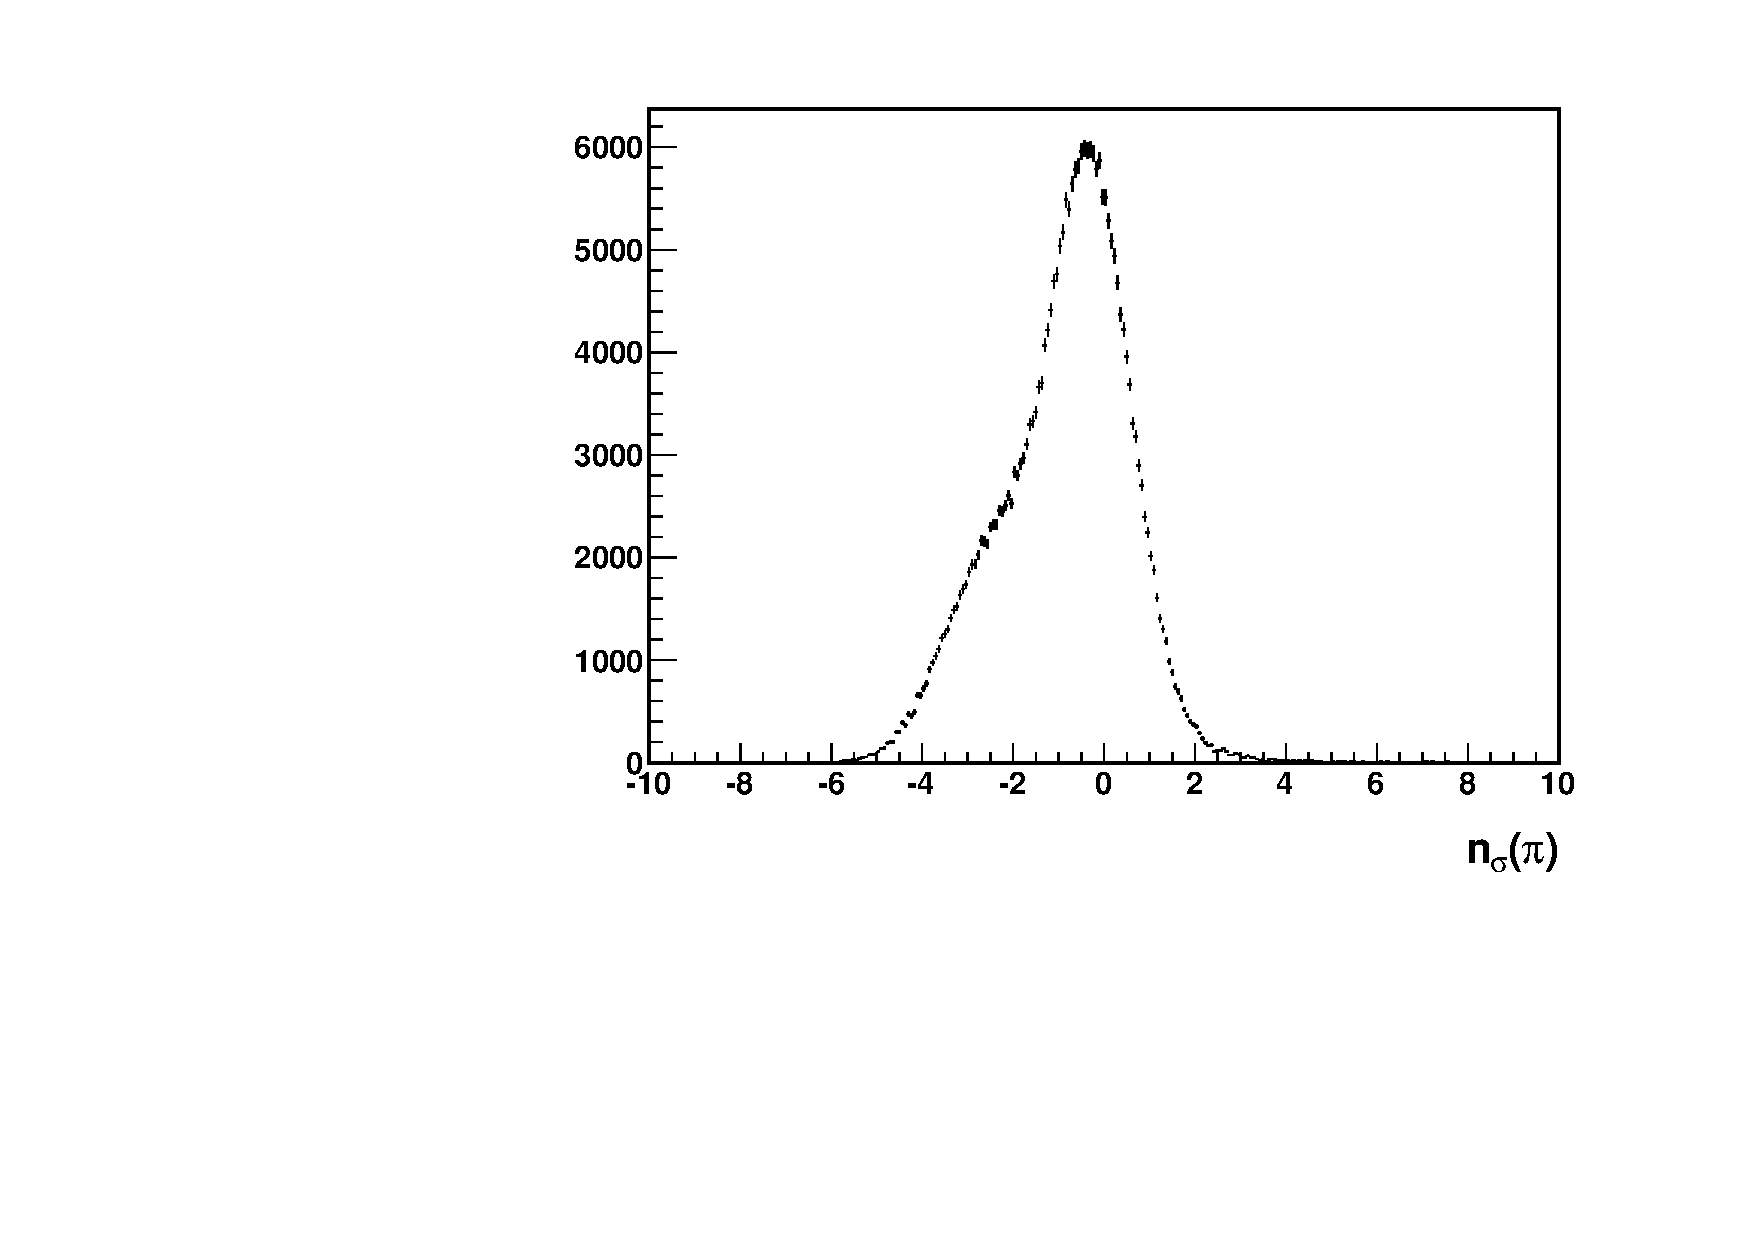
\includegraphics[width = .7\textwidth]{histogramExample.pdf}
\caption[$n_\sigma(\pi)$ distribution]{$n_\sigma(\pi)$ distribution of TPC tracks}
\label{fig:nSigExample}
\end{center}
\end{figure}



 \begin{figure}
\begin{center}
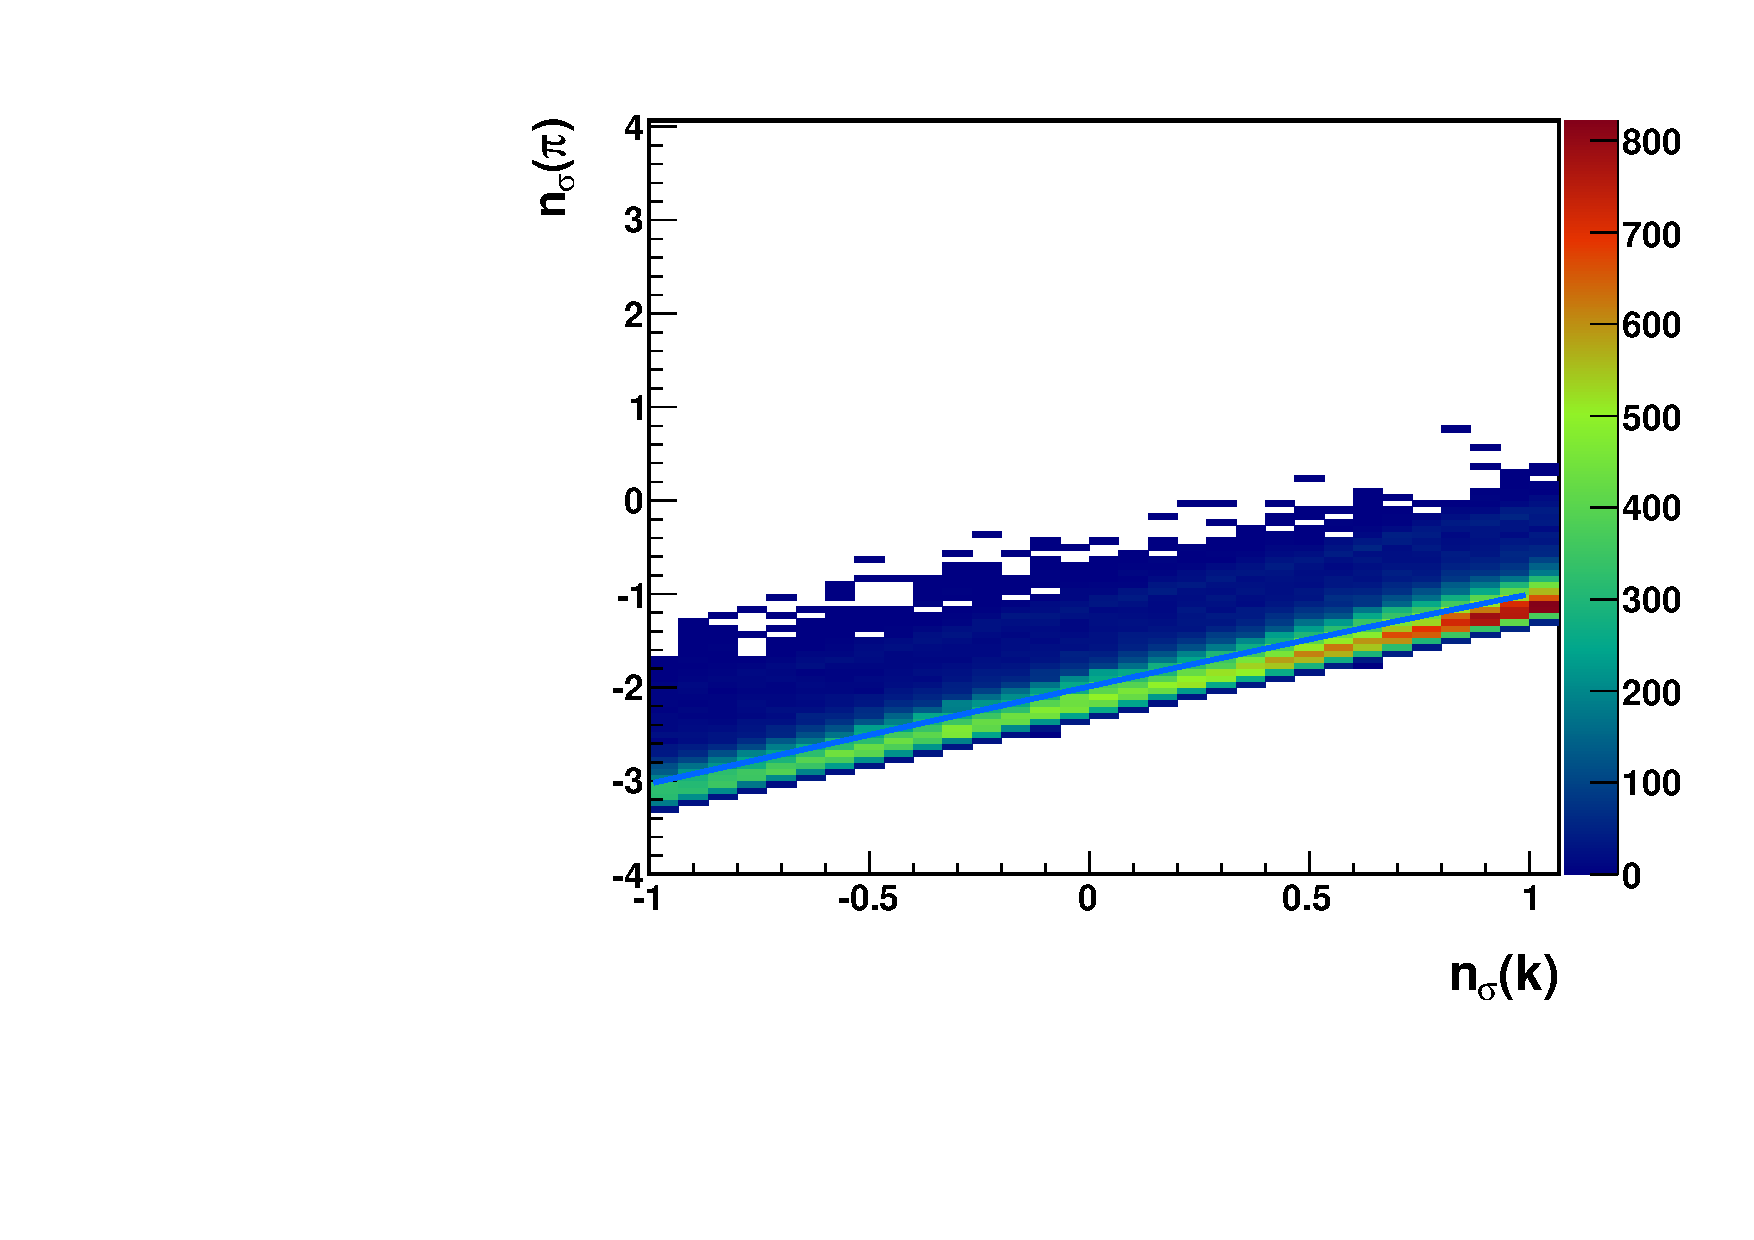
\includegraphics[width = .7\textwidth]{exampleNsigNsig.pdf}
\caption[$n_\sigma(\pi)$ versus $n_\sigma(k)$]{$n_\sigma(\pi)$ versus $n_\sigma(k)$ The blue line is a 3rd order polynomial fit of the profile. The $n_\sigma(\pi)$ value at $n_\sigma(k) = 0$ is taken as the separation between the pion gaussian and the kaon gaussian in the 5-gaussian fit.}
\label{fig:nSignSig}
\end{center}
\end{figure}



 \begin{figure}
\begin{center}
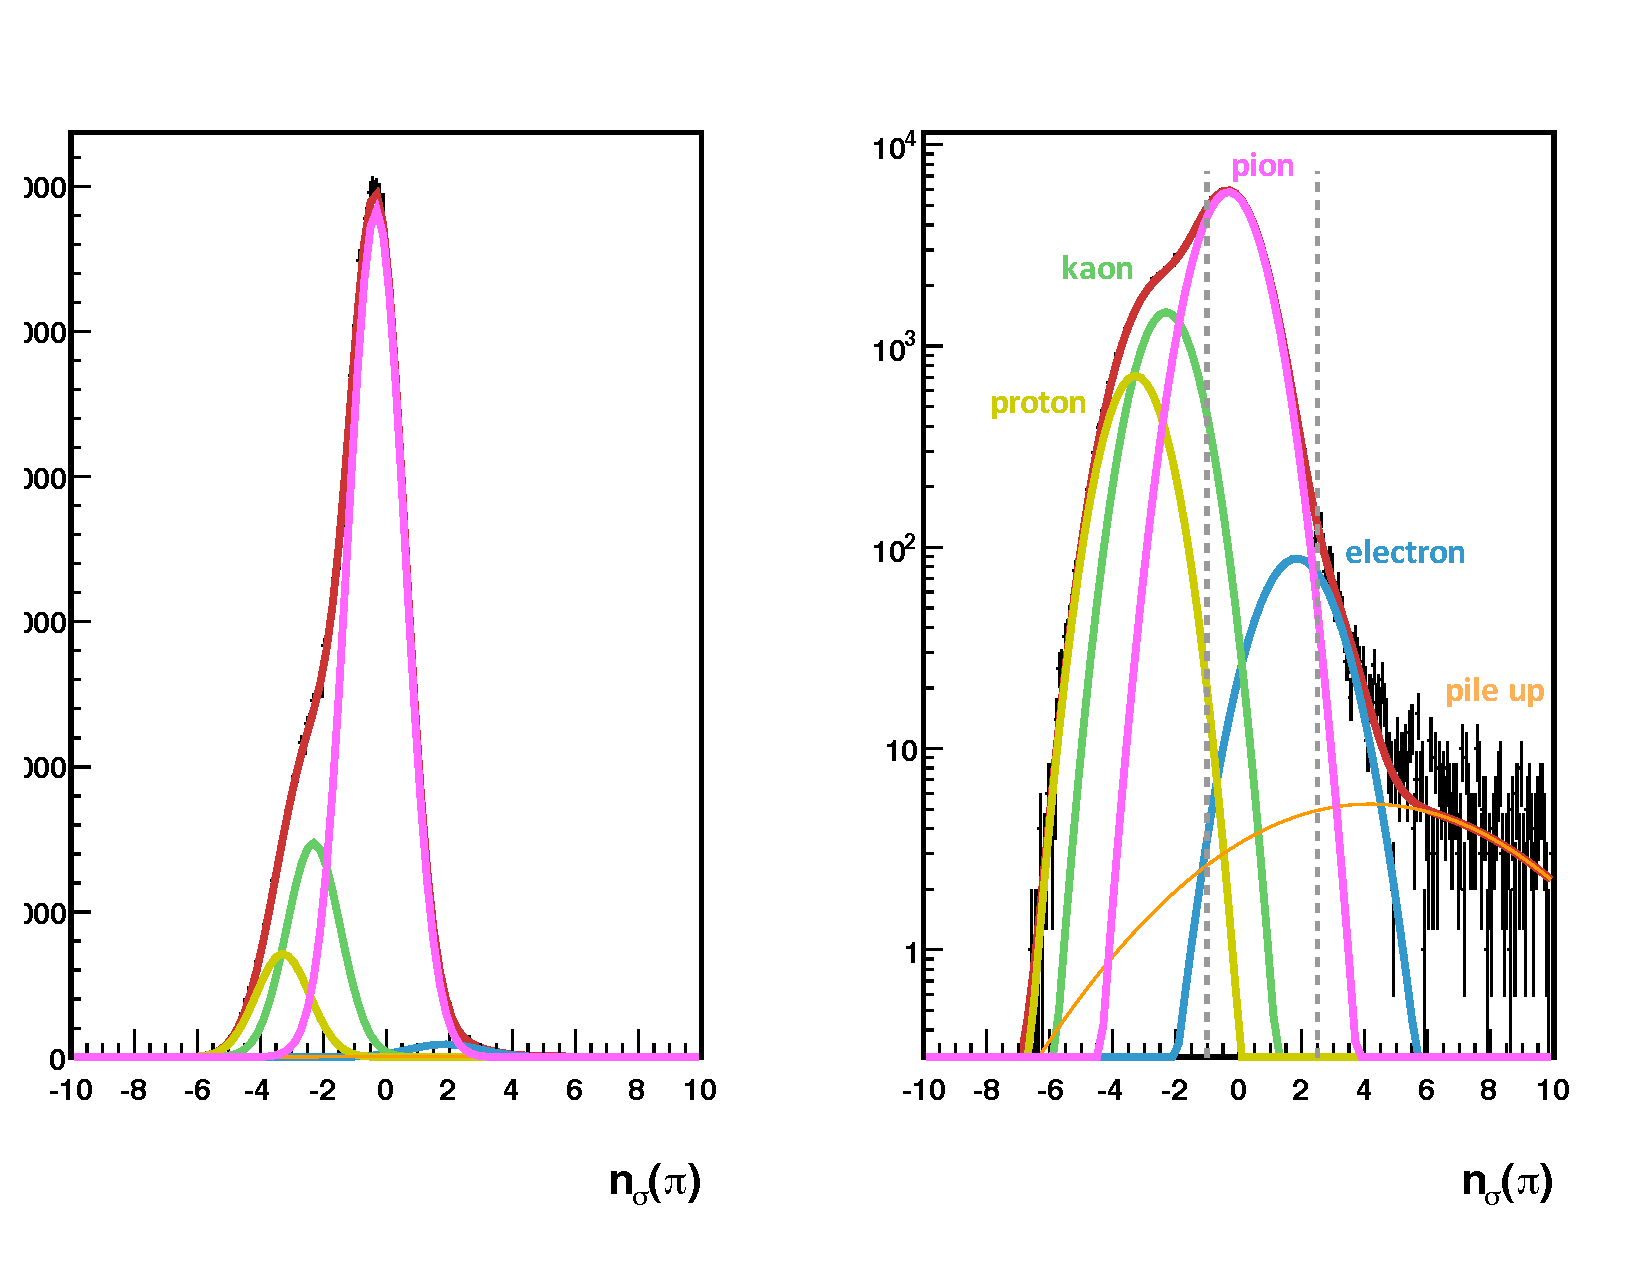
\includegraphics[width = 1\textwidth]{histogramExample2Fit_editFlat2.pdf}
\caption[5-gaussian fit of $n_\sigma(\pi)$ distribution]{5-gaussian fit of $n_\sigma(\pi)$ distribution. The pion peak is shown in pink, the kaon peak in green, the proton peak in yellow, the electron peak in blue, and the pile up peak in orange. Right panel is a log scale for better visibility of smaller peaks. The red line is the sum of all gaussian fits and matches the histogram almost perfectly. The dashed lines indicate the $-1 < n_\sigma(\pi) < 2.5$ range chosen for the analysis.}
\label{fig:nSigExampleFit}
\end{center}
\end{figure}


When teseting interpreting the asymmetry results, it is important to quantify the pion purity of the data. As the ionization energy loss curves show (Fig.~\ref{fig:tpcDedx2}), the energy loss depends on track momentum. More importantly, each particle species displays a different energy loss behavior. Some of these energy loss curves even cross each other at track momentum between 1 and 2 $GeV/c$, making it hard to determine the contamination in the pion data set all at once. Instead the data set is broken into 5 bins in track momentum and 5 in detector $\theta$ (the polar angle measured with respect to the beam direction). In each of these bins, the 5-gaussian fitting procedure is repeated. The 5 gaussian fits are shown in Fig.~\ref{fig:5gaus4} to \ref{fig:5gaus0}. For the four highest track momentum bins, the pion fraction is calculated by integrating the pion gaussian from $n_\sigma(\pi) = -1$ to $n_\sigma(\pi) = 2.5$ and dividing by the integral of the total fit in the same range. As seen in Fig.~\ref{fig:tpcDedx2}, the proton and pion energy loss curves start to overlap in the smallest track momentum bin used ($1.5 \text{ GeV/c} < p < 2.04 \text{ GeV/c}$). This prohibits an accurate determination of the pion fraction using the same method. Luckily in this low momentum range, the time-of-flight can accurately distinguish protons and pions. A two dimensional histogram of $M^2$ versus $n_\sigma(\pi)$ given in Fig.~\ref{fig:tofPlot} shows how the protons are distinguished from pions. Any particle above the red line is taken to be a proton. The proton fraction is then computed by dividing the number of tracks above the red line by the total number of tracks. The kaon, electron, and pile up fractions can still be computed from integrating the 5-gaussian fits, and the pion fraction is determined by the relationship: $1-F_k - F_p - F_e - F_{pile-up} = F_\pi$. 

Since the actual asymmetry analysis is binned in pion pair transverse momentum, invariant mass, and pseudorapidity, we need to find pion fractions for these bins. These purity fractions were computed from the known pion fractions found in the track momentum and detector $\theta$ bins using a weighted mean. The purity values for the analysis binning can be found in tables \ref{tab:1dbinPurity} and \ref{tab:2dbinPurity}. The error for these purity values are on the order of $1\times 10^{-3}$.






 \begin{figure}
\begin{center}
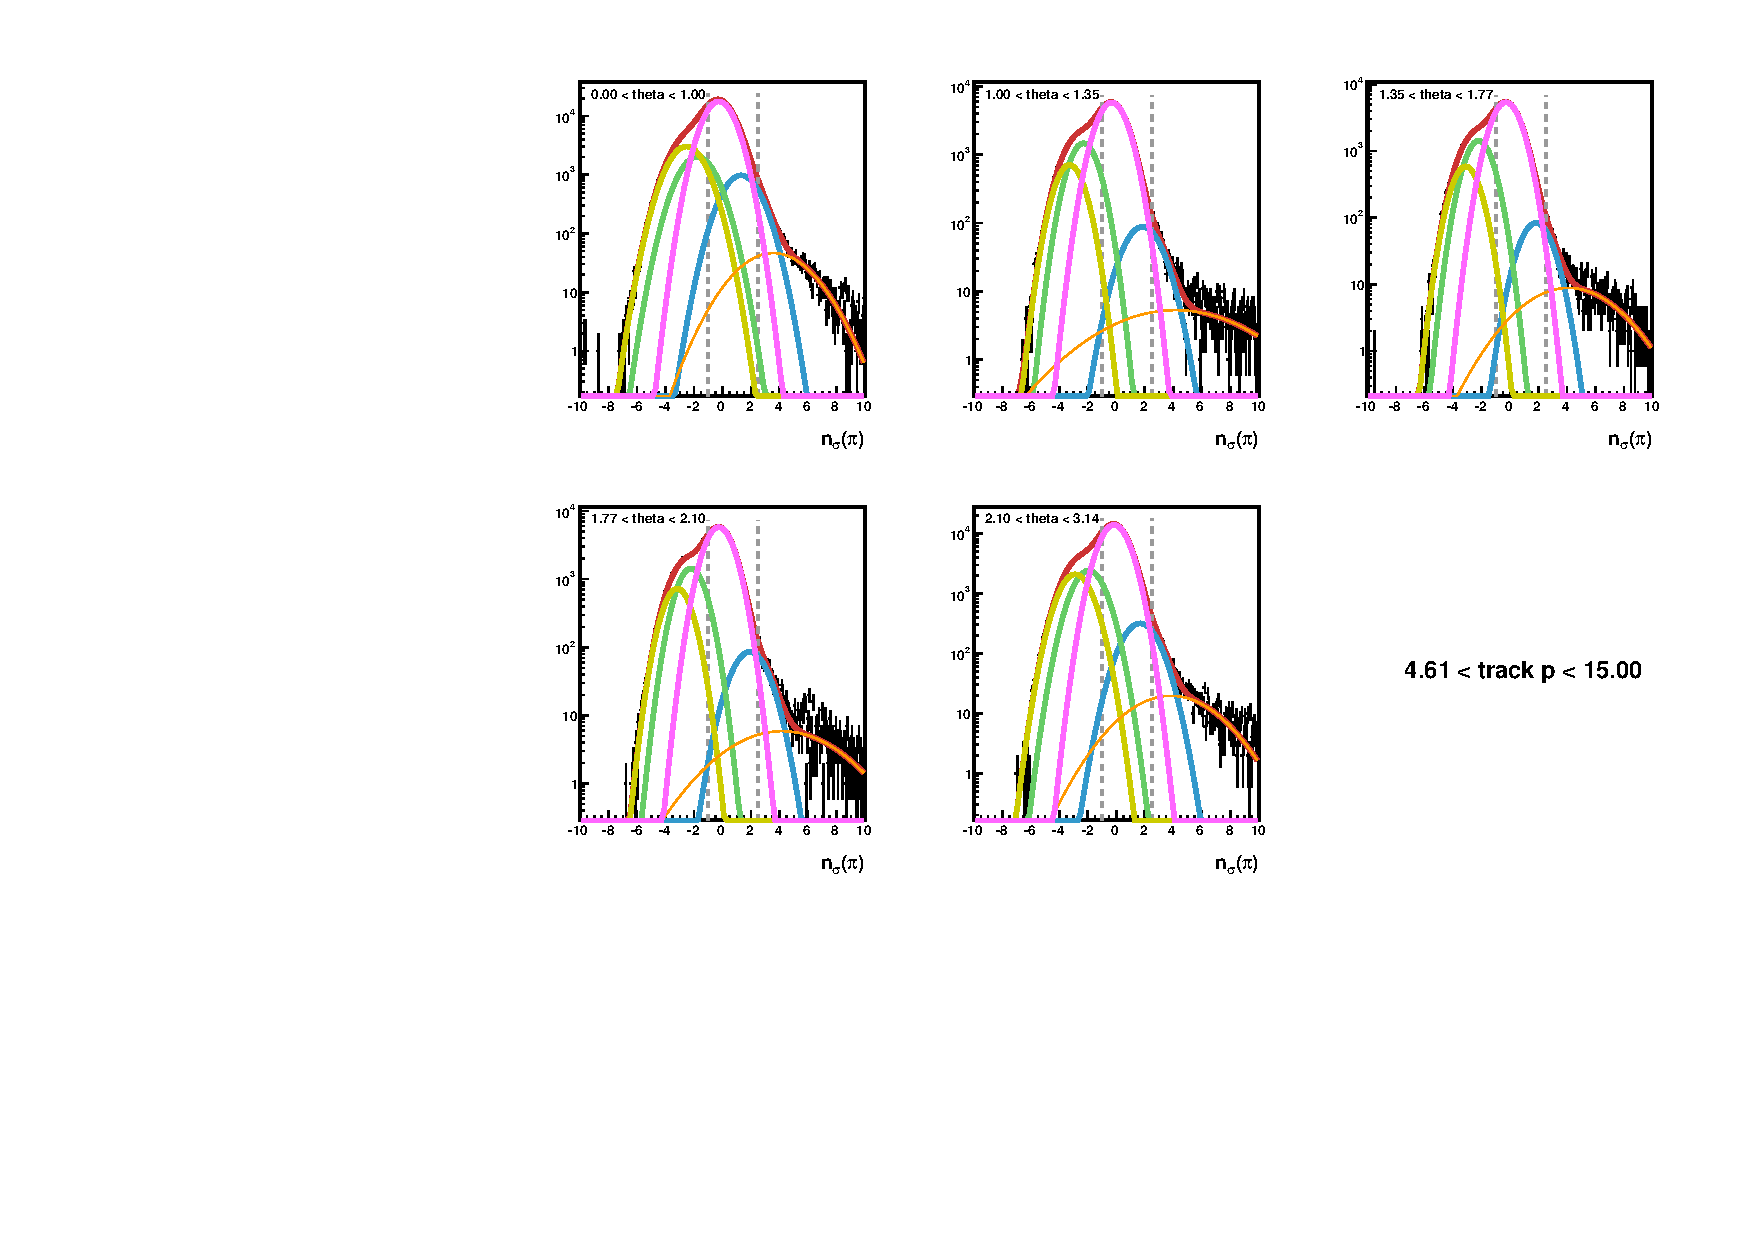
\includegraphics[width = .7\textwidth]{5gausFit_pbin_4.pdf}
\caption[]{}
\label{fig:5gaus4}
\end{center}
\end{figure}

 \begin{figure}
\begin{center}
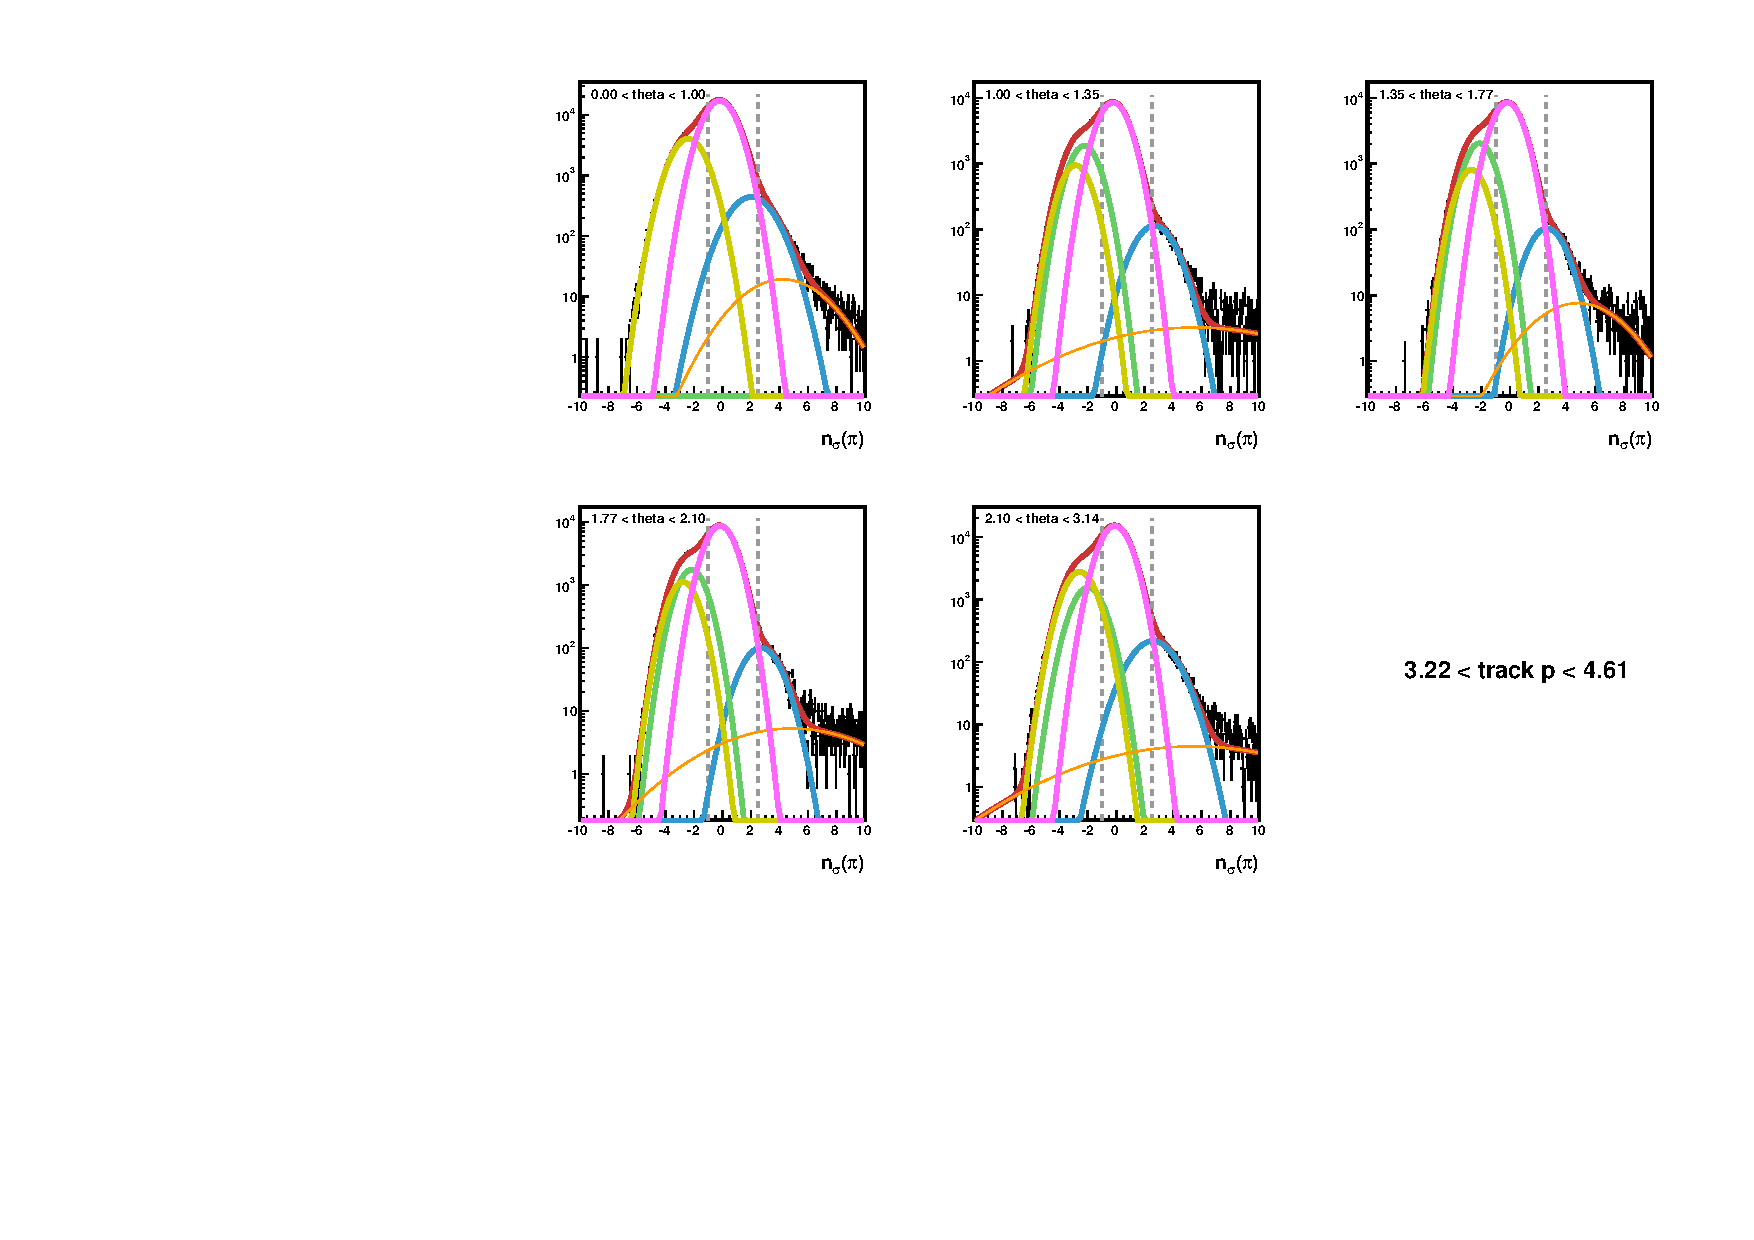
\includegraphics[width = .7\textwidth]{5gausFit_pbin_3.pdf}
\caption[]{}
\label{fig:5gaus3}
\end{center}
\end{figure}

 \begin{figure}
\begin{center}
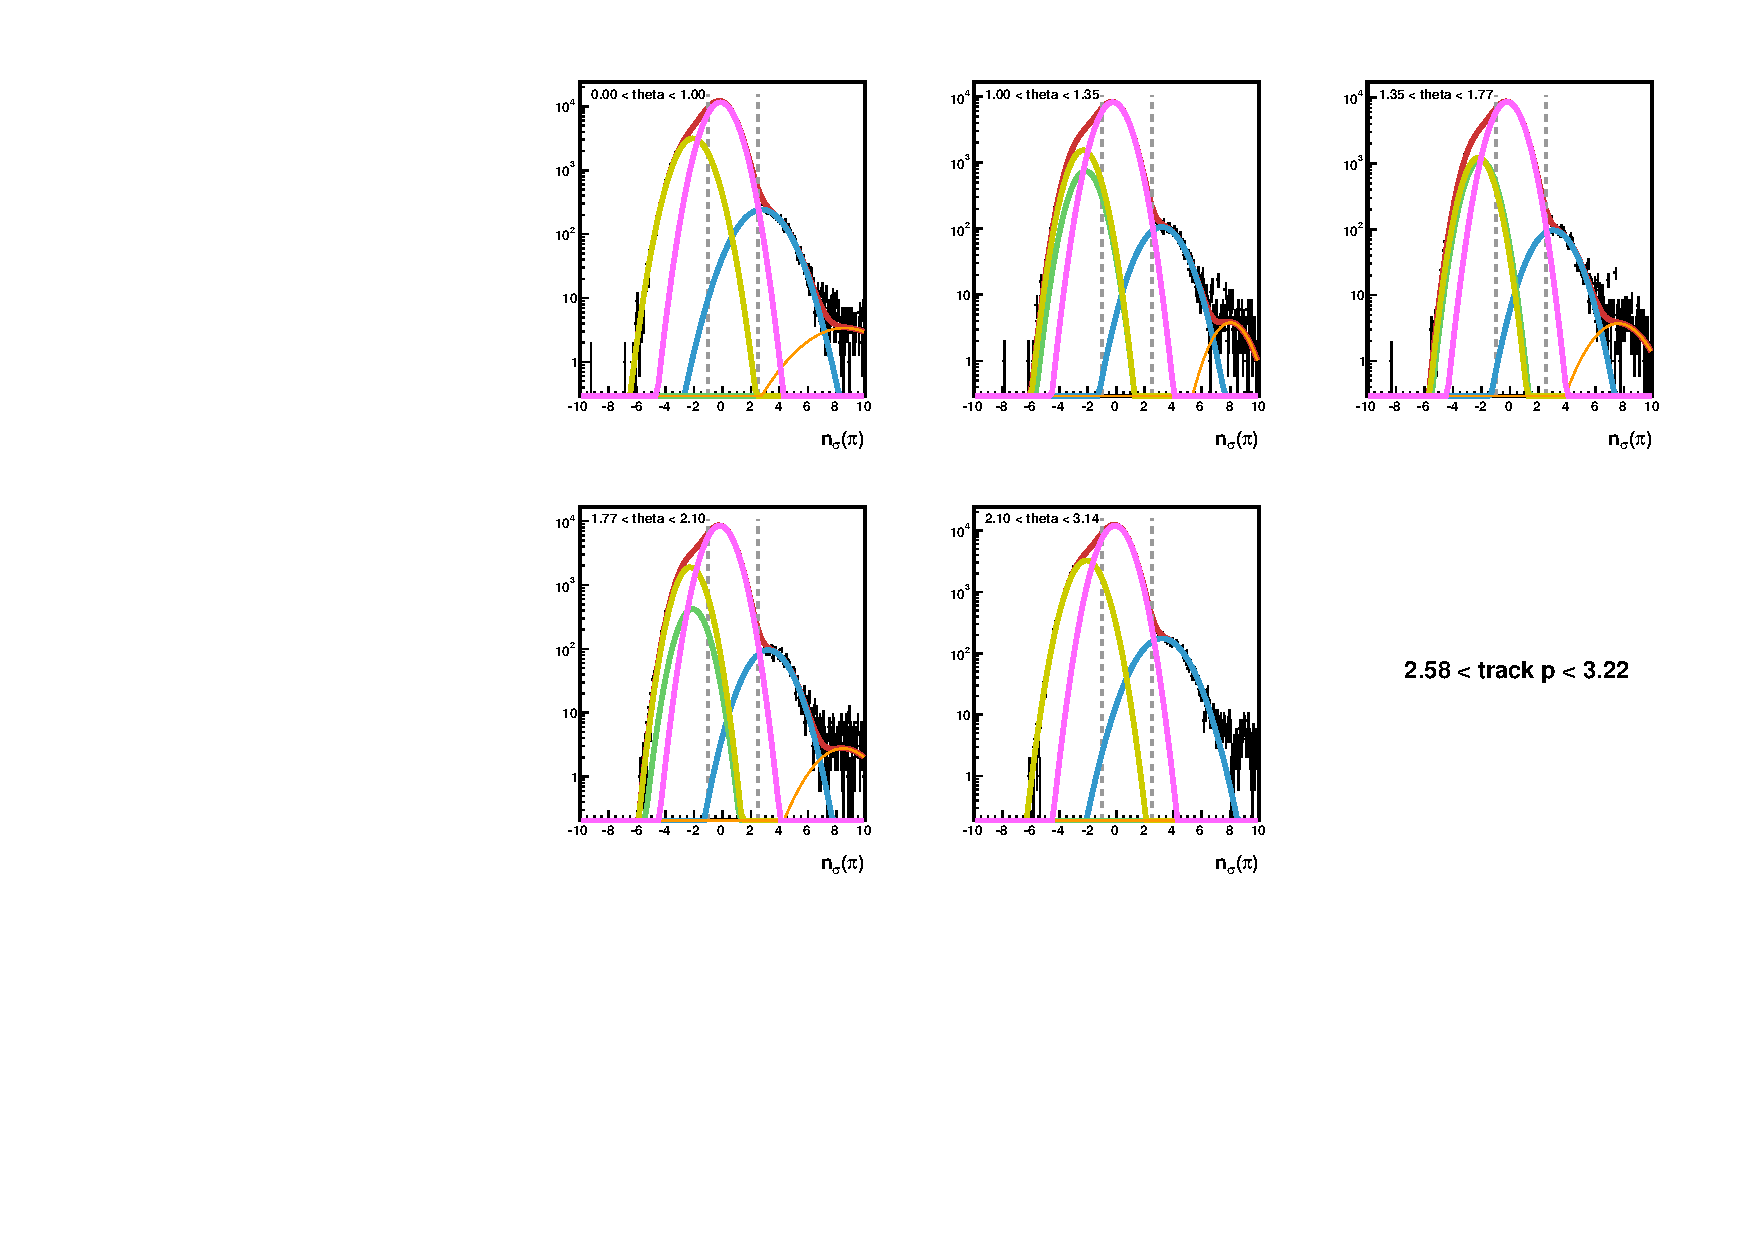
\includegraphics[width = .7\textwidth]{5gausFit_pbin_2.pdf}
\caption[]{}
\label{fig:5gaus2}
\end{center}
\end{figure}

 \begin{figure}
\begin{center}
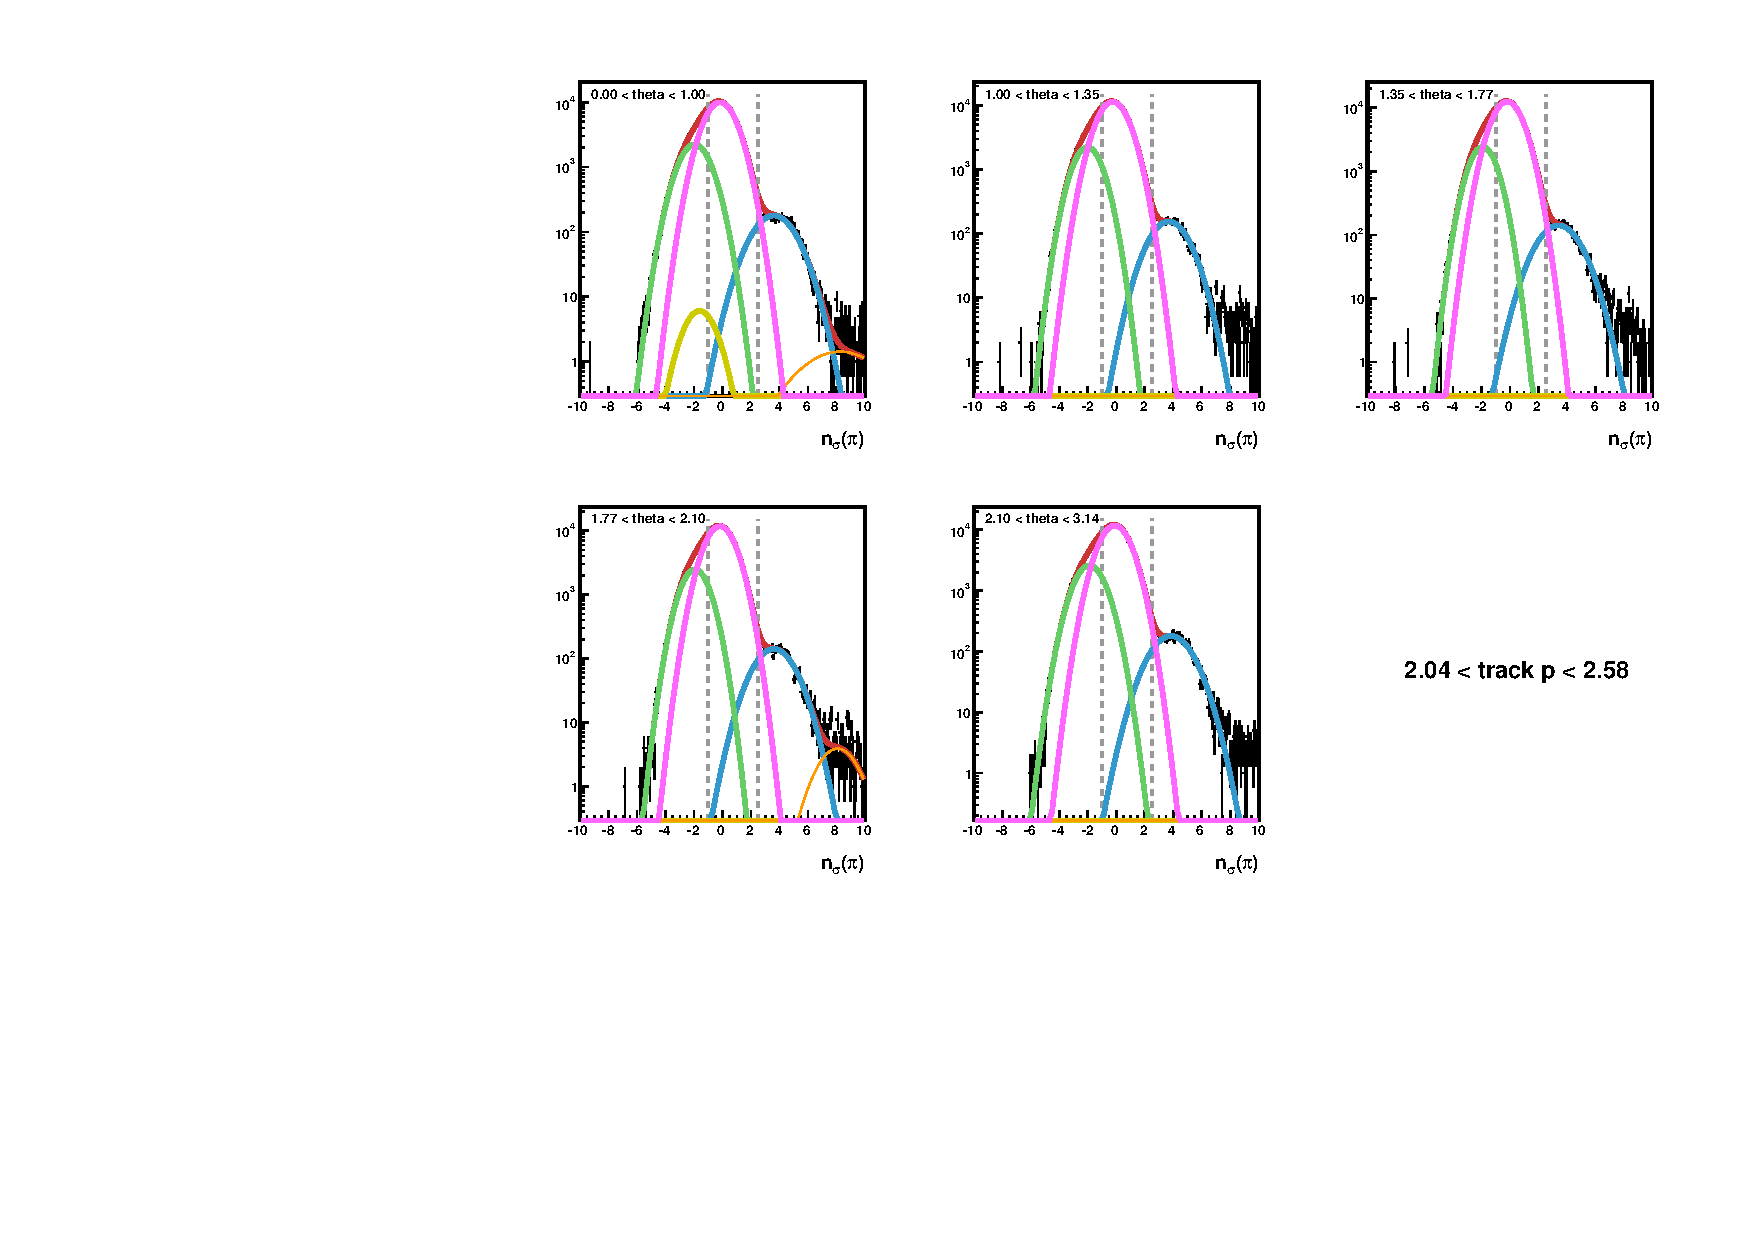
\includegraphics[width = .7\textwidth]{5gausFit_pbin_1.pdf}
\caption[]{}
\label{fig:5gaus1}
\end{center}
\end{figure}

 \begin{figure}
\begin{center}
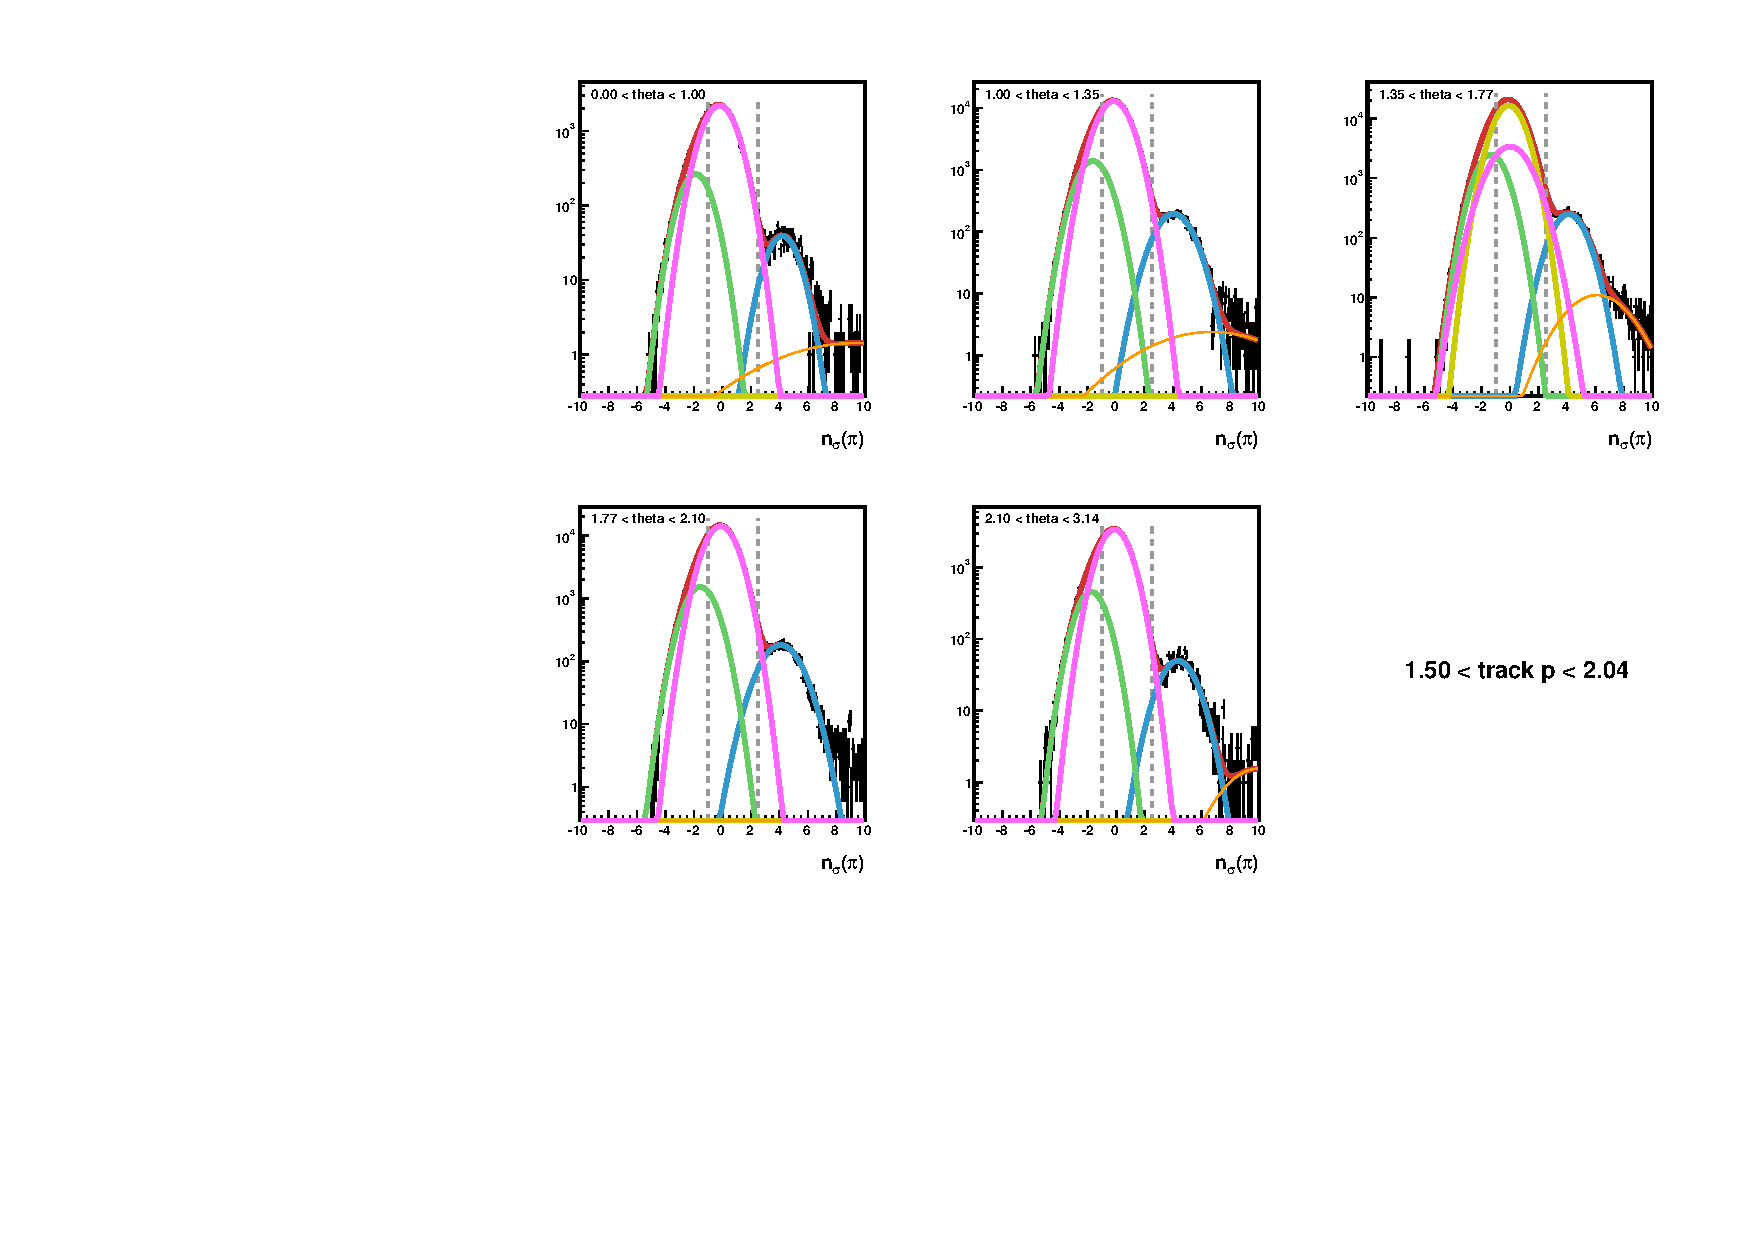
\includegraphics[width = .7\textwidth]{5gausFit_pbin_0.pdf}
\caption[]{}
\label{fig:5gaus0}
\end{center}
\end{figure}

 \begin{figure}
\begin{center}
\includegraphics[width = .7\textwidth]{tofPlot.pdf}
\caption[]{}
\label{fig:tofPlot}
\end{center}
\end{figure}


\begin{table}[!h]
\tiny
	\caption{pion purity for 1D binning}
	\label{tab:1dbinPurity}
\begin{minipage}{.33\linewidth}
		%\caption{purity in $\etapair$}
		%\hline
\begin{tabularx}{\textwidth}{@{}YY@{}}
		$\etapair$ & pion \%  \\
		\hline
		-2.00 $-$ -0.60 & 95\\
		-0.60 $-$ -0.30 & 95\\
		-0.30 $-$ 0.00 & 95\\
		0.00 $-$ 0.40 & 95\\
		0.40 $-$ 0.75 & 95\\
		0.75 $-$ 2.00 & 92\\
		\\
		\\
		\\
		\hline
		\end{tabularx}
	\end{minipage}%
\begin{minipage}{.33\linewidth}
		%\caption{purity in $\mpair$}
		%\hline
\begin{tabularx}{\textwidth}{@{}|YY|@{}}
		$\mpair$ & pion \%  \\
		\hline
0.00 $-$ 0.38 & 94\\
0.38 $-$ 0.44 & 94\\
0.44 $-$ 0.50 & 94\\
0.50 $-$ 0.56 & 94\\
0.56 $-$ 0.62 & 95\\
0.62 $-$ 0.72 & 95\\
0.72 $-$ 0.86 & 95\\
0.86 $-$ 1.10 & 94\\
1.10 $-$ 100  & 94\\
		\hline
		\end{tabularx}
	\end{minipage}%
\begin{minipage}{.33\linewidth}
		%\caption{purity in $\ptpair$}
		%\hline
\begin{tabularx}{\textwidth}{@{}YY@{}}
		$\ptpair$ & pion  \% \\
		\hline
3.00 $-$ 3.70 & 93\\
3.70 $-$ 4.15 & 95\\
4.15 $-$ 4.63 & 95\\
4.63 $-$ 5.19 & 95\\
5.19 $-$ 5.87 & 95\\
5.87 $-$ 6.80 & 95\\
6.80 $-$ 7.80 & 94\\
7.80 $-$ 10.00 & 94\\
10.00 $-$ 50.00 & 94\\
		\hline
		\end{tabularx}
	\end{minipage}
\end{table}


\begin{table}[!h]
\tiny
	\caption{pion purity for 2D binning}
	\label{tab:2dbinPurity}
\begin{minipage}[t]{.33\linewidth}
		%\caption{\small purity in \\ $\mpair,\etapair$}
		\begin{tabular}[t]{ccc}%\hline
		$\mpair$  & $\etapair$  & pion \%  \\
		\hline
0.00 $ - $ 0.40 & -2.00 $-$ -0.50 & 96\\
0.00 $-$ 0.40 & -0.50 $-$ 0.00 & 94\\
0.00 $-$ 0.40 & 0.00 $-$ 0.50 & 94\\
0.00 $-$ 0.40 & 0.50 $-$ 2.00 & 94\\
0.40 $-$ 0.60 & -2.00 $-$ -0.50 & 96\\
0.40 $-$ 0.60 & -0.50 $-$ 0.00 & 94\\
0.40 $-$ 0.60 & 0.00 $-$ 0.50 & 94\\
0.40 $-$ 0.60 & 0.50 $-$ 2.00 & 94\\
0.60 $-$ 0.80 & -2.00 $-$ -0.50 & 96\\
0.60 $-$ 0.80 & -0.50 $-$ 0.00 & 94\\
0.60 $-$ 0.80 & 0.00 $-$ 0.50 & 94\\
0.60 $-$ 0.80 & 0.50 $-$ 2.00 & 94\\
0.80 $-$ 1.00 & -2.00 $-$ -0.50 & 96\\
0.80 $-$ 1.00 & -0.50 $-$ 0.00 & 94\\
0.80 $-$ 1.00 & 0.00 $-$ 0.50 & 94\\
0.80 $-$ 1.00 & 0.50 $-$ 2.00 & 94\\
1.00 $-$ 100.50 & -2.00 $-$ -0.50 & 96\\
1.00 $-$ 100.50 & -0.50 $-$ 0.00 & 95\\
1.00 $-$ 100.50 & 0.00 $-$ 0.50 & 94\\
1.00 $-$ 100.50 & 0.50 $-$ 2.00 & 94\\
\\
\\
\\
\\
\\		
		\hline
		\end{tabular}
	\end{minipage}%
\begin{minipage}[t]{.33\linewidth}
		%\caption{\small purity in \\ $\mpair,\ptpair$}
		\begin{tabular}[t]{|ccc|}%\hline
		$\mpair$  & $\ptpair$  & pion \%  \\
		\hline
3.00 $-$ 4.00 & 0.00 $-$ 0.40 & 94\\
3.00 $-$ 4.00 & 0.40 $-$ 0.60 & 94\\
3.00 $-$ 4.00 & 0.60 $-$ 0.80 & 94\\
3.00 $-$ 4.00 & 0.80 $-$ 1.00 & 94\\
3.00 $-$ 4.00 & 1.00 $-$ 100.50 & 94\\
4.00 $-$ 5.00 & 0.00 $-$ 0.40 & 94\\
4.00 $-$ 5.00 & 0.40 $-$ 0.60 & 94\\
4.00 $-$ 5.00 & 0.60 $-$ 0.80 & 94\\
4.00 $-$ 5.00 & 0.80 $-$ 1.00 & 94\\
4.00 $-$ 5.00 & 1.00 $-$ 100.50 & 94\\
5.00 $-$ 6.50 & 0.00 $-$ 0.40 & 95\\
5.00 $-$ 6.50 & 0.40 $-$ 0.60 & 94\\
5.00 $-$ 6.50 & 0.60 $-$ 0.80 & 94\\
5.00 $-$ 6.50 & 0.80 $-$ 1.00 & 94\\
5.00 $-$ 6.50 & 1.00 $-$ 100.50 & 94\\
6.50 $-$ 8.00 & 0.00 $-$ 0.40 & 94\\
6.50 $-$ 8.00 & 0.40 $-$ 0.60 & 94\\
6.50 $-$ 8.00 & 0.60 $-$ 0.80 & 94\\
6.50 $-$ 8.00 & 0.80 $-$ 1.00 & 94\\
6.50 $-$ 8.00 & 1.00 $-$ 100.50 & 94\\
8.00 $-$ 50.00 & 0.00 $-$ 0.40 & 94\\
8.00 $-$ 50.00 & 0.40 $-$ 0.60 & 94\\
8.00 $-$ 50.00 & 0.60 $-$ 0.80 & 94\\
8.00 $-$ 50.00 & 0.80 $-$ 1.00 & 94\\
8.00 $-$ 50.00 & 1.00 $-$ 100.50 & 94\\
		\hline
		\end{tabular}
	\end{minipage}%
\begin{minipage}[t]{.33\linewidth}
		%\caption{\small purity in \\ $\ptpair,\etapair$}
		\begin{tabular}[t]{ccc}%\hline
		$\ptpair$  & $\etapair$  & pion \%  \\
		\hline
		3.00 $-$ 4.00 & -2.00 $-$ -0.50 & 95\\
3.00 $-$ 4.00 & -0.50 $-$ 0.00 & 93\\
3.00 $-$ 4.00 & 0.00 $-$ 0.50 & 93\\
3.00 $-$ 4.00 & 0.50 $-$ 2.00 & 94\\
4.00 $-$ 5.00 & -2.00 $-$ -0.50 & 96\\
4.00 $-$ 5.00 & -0.50 $-$ 0.00 & 95\\
4.00 $-$ 5.00 & 0.00 $-$ 0.50 & 94\\
4.00 $-$ 5.00 & 0.50 $-$ 2.00 & 94\\
5.00 $-$ 6.50 & -2.00 $-$ -0.50 & 96\\
5.00 $-$ 6.50 & -0.50 $-$ 0.00 & 95\\
5.00 $-$ 6.50 & 0.00 $-$ 0.50 & 94\\
5.00 $-$ 6.50 & 0.50 $-$ 2.00 & 94\\
6.50 $-$ 8.00 & -2.00 $-$ -0.50 & 96\\
6.50 $-$ 8.00 & -0.50 $-$ 0.00 & 94\\
6.50 $-$ 8.00 & 0.00 $-$ 0.50 & 94\\
6.50 $-$ 8.00 & 0.50 $-$ 2.00 & 94\\
8.00 $-$ 50.00 & -2.00 $-$ -0.50 & 95\\
8.00 $-$ 50.00 & -0.50 $-$ 0.00 & 94\\
8.00 $-$ 50.00 & 0.00 $-$ 0.50 & 93\\
8.00 $-$ 50.00 & 0.50 $-$ 2.00 & 94\\
\\
\\
\\
\\
\\		
		\hline
		\end{tabular}
	\end{minipage}
\end{table}




%\begin{table}[!h]
%\tiny
%	\caption{pion purity for 2D binning}
%	\label{tab:2dbinPurity}
%\begin{minipage}[t]{.33\linewidth}
%		%\caption{\small purity in \\ $\mpair,\etapair$}
%		\begin{tabularx}{\textwidth}{@{}YYY@{}}\hline
%		$\mpair$  & $\etapair$  & pion \%  \\
%		\hline
%0.00 $ - $ 0.40 & -2.00 $-$ -0.50 & 96\\
%0.00 $-$ 0.40 & -0.50 $-$ 0.00 & 94\\
%0.00 $-$ 0.40 & 0.00 $-$ 0.50 & 94\\
%0.00 $-$ 0.40 & 0.50 $-$ 2.00 & 94\\
%0.40 $-$ 0.60 & -2.00 $-$ -0.50 & 96\\
%0.40 $-$ 0.60 & -0.50 $-$ 0.00 & 94\\
%0.40 $-$ 0.60 & 0.00 $-$ 0.50 & 94\\
%0.40 $-$ 0.60 & 0.50 $-$ 2.00 & 94\\
%0.60 $-$ 0.80 & -2.00 $-$ -0.50 & 96\\
%0.60 $-$ 0.80 & -0.50 $-$ 0.00 & 94\\
%0.60 $-$ 0.80 & 0.00 $-$ 0.50 & 94\\
%0.60 $-$ 0.80 & 0.50 $-$ 2.00 & 94\\
%0.80 $-$ 1.00 & -2.00 $-$ -0.50 & 96\\
%0.80 $-$ 1.00 & -0.50 $-$ 0.00 & 94\\
%0.80 $-$ 1.00 & 0.00 $-$ 0.50 & 94\\
%0.80 $-$ 1.00 & 0.50 $-$ 2.00 & 94\\
%1.00 $-$ 100.50 & -2.00 $-$ -0.50 & 96\\
%1.00 $-$ 100.50 & -0.50 $-$ 0.00 & 95\\
%1.00 $-$ 100.50 & 0.00 $-$ 0.50 & 94\\
%1.00 $-$ 100.50 & 0.50 $-$ 2.00 & 94\\
%\\
%\\
%\\
%\\
%\\		
%		\hline
%		\end{tabularx}
%	\end{minipage}%
%\begin{minipage}[t]{.33\linewidth}
%		%\caption{\small purity in \\ $\mpair,\ptpair$}
%		\begin{tabularx}{\textwidth}{@{}|YYY|@{}}\hline
%		$\mpair$  & $\ptpair$  & pion \%  \\
%		\hline
%3.00 $-$ 4.00 & 0.00 $-$ 0.40 & 94\\
%3.00 $-$ 4.00 & 0.40 $-$ 0.60 & 94\\
%3.00 $-$ 4.00 & 0.60 $-$ 0.80 & 94\\
%3.00 $-$ 4.00 & 0.80 $-$ 1.00 & 94\\
%3.00 $-$ 4.00 & 1.00 $-$ 100.50 & 94\\
%4.00 $-$ 5.00 & 0.00 $-$ 0.40 & 94\\
%4.00 $-$ 5.00 & 0.40 $-$ 0.60 & 94\\
%4.00 $-$ 5.00 & 0.60 $-$ 0.80 & 94\\
%4.00 $-$ 5.00 & 0.80 $-$ 1.00 & 94\\
%4.00 $-$ 5.00 & 1.00 $-$ 100.50 & 94\\
%5.00 $-$ 6.50 & 0.00 $-$ 0.40 & 95\\
%5.00 $-$ 6.50 & 0.40 $-$ 0.60 & 94\\
%5.00 $-$ 6.50 & 0.60 $-$ 0.80 & 94\\
%5.00 $-$ 6.50 & 0.80 $-$ 1.00 & 94\\
%5.00 $-$ 6.50 & 1.00 $-$ 100.50 & 94\\
%6.50 $-$ 8.00 & 0.00 $-$ 0.40 & 94\\
%6.50 $-$ 8.00 & 0.40 $-$ 0.60 & 94\\
%6.50 $-$ 8.00 & 0.60 $-$ 0.80 & 94\\
%6.50 $-$ 8.00 & 0.80 $-$ 1.00 & 94\\
%6.50 $-$ 8.00 & 1.00 $-$ 100.50 & 94\\
%8.00 $-$ 50.00 & 0.00 $-$ 0.40 & 94\\
%8.00 $-$ 50.00 & 0.40 $-$ 0.60 & 94\\
%8.00 $-$ 50.00 & 0.60 $-$ 0.80 & 94\\
%8.00 $-$ 50.00 & 0.80 $-$ 1.00 & 94\\
%8.00 $-$ 50.00 & 1.00 $-$ 100.50 & 94\\
%		\hline
%		\end{tabularx}
%	\end{minipage}%
%\begin{minipage}[t]{.33\linewidth}
%		%\caption{\small purity in \\ $\ptpair,\etapair$}
%		\begin{tabularx}{\textwidth}{@{}YYY@{}}\hline
%		$\ptpair$  & $\etapair$  & pion \%  \\
%		\hline
%		3.00 $-$ 4.00 & -2.00 $-$ -0.50 & 95\\
%3.00 $-$ 4.00 & -0.50 $-$ 0.00 & 93\\
%3.00 $-$ 4.00 & 0.00 $-$ 0.50 & 93\\
%3.00 $-$ 4.00 & 0.50 $-$ 2.00 & 94\\
%4.00 $-$ 5.00 & -2.00 $-$ -0.50 & 96\\
%4.00 $-$ 5.00 & -0.50 $-$ 0.00 & 95\\
%4.00 $-$ 5.00 & 0.00 $-$ 0.50 & 94\\
%4.00 $-$ 5.00 & 0.50 $-$ 2.00 & 94\\
%5.00 $-$ 6.50 & -2.00 $-$ -0.50 & 96\\
%5.00 $-$ 6.50 & -0.50 $-$ 0.00 & 95\\
%5.00 $-$ 6.50 & 0.00 $-$ 0.50 & 94\\
%5.00 $-$ 6.50 & 0.50 $-$ 2.00 & 94\\
%6.50 $-$ 8.00 & -2.00 $-$ -0.50 & 96\\
%6.50 $-$ 8.00 & -0.50 $-$ 0.00 & 94\\
%6.50 $-$ 8.00 & 0.00 $-$ 0.50 & 94\\
%6.50 $-$ 8.00 & 0.50 $-$ 2.00 & 94\\
%8.00 $-$ 50.00 & -2.00 $-$ -0.50 & 95\\
%8.00 $-$ 50.00 & -0.50 $-$ 0.00 & 94\\
%8.00 $-$ 50.00 & 0.00 $-$ 0.50 & 93\\
%8.00 $-$ 50.00 & 0.50 $-$ 2.00 & 94\\
%\\
%\\
%\\
%\\
%\\		
%		\hline
%		\end{tabularx}
%	\end{minipage}
%\end{table}




\section{Finding $\pi^+\pi^-$ Pairs}

%\begin{figure}
%\begin{center}
%\includegraphics[width = .7\textwidth]{starPic6}
%\caption[Schematic of Analysis]{}
%\label{fig:analSchem}
%\end{center}
%\end{figure}


\begin{figure}
	\caption{Schematic of Analysis}
	\begin{tabular}{cc}
	\subfloat[pion pair produced in collision]{\includegraphics[width=.7\textwidth]{starPic6}\label{fig:pairInEvent}} & \subfloat[radius check on pion pair]{\includegraphics[width=.3\textwidth]{coneNew3}\label{fig:radCheck}} 
	\end{tabular}
\end{figure}


%\begin{figure}
%\begin{center}
%\includegraphics[width = 1\textwidth]{dedxforPID}
%\caption[Ionization energy loss in TPC gas on log scale]{ionization energy loss $vs$ momentum in TPC. Tracks in the red band are pions we want to consider for analysis. The blue and pink bands are kaons and protons, respectively, that we want minimize in our sample.}
%\label{fig:dedx}
%\end{center}
%\end{figure}


%\begin{figure}
%\begin{center}
%\includegraphics[width = 1\textwidth]{nSigma_05_1}
%\caption[$\nsigpi$ distribution and triple Gaussian fit]{Distribution of $\nsigpi$ fit with three Gaussians.}
%\label{fig:nSigPiCut}
%\end{center}
%\end{figure}

%\begin{figure}
%\begin{center}
%\includegraphics[width = 1\textwidth]{nSigmaVsEta_witherrors.pdf}
%\caption[Contamination of pion sample]{contamination from kaon, proton, and electron}
%\label{fig:contamination}
%\end{center}
%\end{figure}

Once a clean pion sample is found, $\pi^+$s and $\pi^-$s must be combined into $\pi^+\pi^-$ pairs. An example of an event of interest can be seen in Fig.~\ref{fig:pairInEvent}. Here we see a positively charged pion and negatively charged pion produced in close proximity by the proton collision. This is what we refer to as a pion pair.  Every combination of $\pi^+$ and $\pi^-$ in an event is checked. Since the two pions are required to be from the same fragmenting quark, they are taken as a pair and used in the analysis if they pass the individual track cuts and if they are contained in a cone of a certain radius in $\eta-\phi$ space (Fig.~\ref{fig:radCheck}). For 1D binning, radii of 0.2, 0.3, and 0.4 are used, while 0.7 is used in 2D binning in order to increase statistics. Even the largest of these radii should still be effective to ensure the the two pions are from the same fragmenting quark.  

%\begin{figure}
%\begin{center}
%\includegraphics[width = 1\textwidth]{coneNew3}
%\caption[Radius cut]{radius cut}
%\label{fig:radCut}
%\end{center}
%\end{figure}

\FloatBarrier
\section{Pair Distributions}

The entire data set provides 17544516 $\pi^+\pi^-$ pairs in a radius between 0.05 and 1.0 in $\eta,\phi$ space before trigger information is used. The minimum radius cut of 0.05 is used because when the tracks are very close together, the uncertainty in track position can cause the orientation of the pairs to flip. Since the orientation of the pair is so important to the observed asymmetry, this is unacceptable for our analysis. 


Once the data set was ready, quality tests were performed on the pion pairs. These included looking at the invariant mass, transverse momentum, and pseudorapidity distributions for the pairs. Quality control plots of relevant kinematic variables of individual pions and pion pairs with a maximum radius of 0.3 can be seen in Figs.~\ref{fig:posPt} to \ref{fig:cosTheta}. 

\FloatBarrier
\begin{figure}
\begin{center}
\includegraphics[width = .8\textwidth]{hPosPt}
\caption[$P_{T}$ distribution of $\pi^+$]{$P_{T}$ distribution of $\pi^+$}
\label{fig:posPt}
\end{center}
\end{figure}

\begin{figure}
\begin{center}
\includegraphics[width = .8\textwidth]{hNegPt}
\caption[$P_{T}$ distribution of $\pi^-$]{$P_{T}$ distribution of $\pi^-$}
\label{fig:negpt}
\end{center}
\end{figure}

\begin{figure}
\begin{center}
\includegraphics[width = .8\textwidth]{hPosPhi}
\caption[$\phi$ distribution of $\pi^+$]{$\phi$ distribution of $\pi^+$}
\label{fig:posphi}
\end{center}
\end{figure}

\begin{figure}
\begin{center}
\includegraphics[width = .8\textwidth]{hNegPhi}
\caption[$\phi$ distribution of $\pi^-$]{$\phi$ distribution of $\pi^-$}
\label{fig:negphi}
\end{center}
\end{figure}

\begin{figure}
\begin{center}
\includegraphics[width = .8\textwidth]{hPosEta}
\caption[$\eta$ distribution of $\pi^+$]{$\eta$ distribution of $\pi^+$}
\label{fig:poseta}
\end{center}
\end{figure}

\begin{figure}
\begin{center}
\includegraphics[width = .8\textwidth]{hNegEta}
\caption[$\eta$ distribution of $\pi^-$]{$\eta$ distribution of $\pi^-$}
\label{fig:negeta}
\end{center}
\end{figure}

\begin{figure}
\begin{center}
\includegraphics[width = .8\textwidth]{hPtPair}
\caption[$P_{T}$ distribution of \pair pair]{$P_{T}$ distribution of \pair pair}
\label{fig:pt}
\end{center}
\end{figure}

\begin{figure}
\begin{center}
\includegraphics[width = .8\textwidth]{hPhiPair}
\caption[$\phi$ distribution of \pair pair]{$\phi$ distribution of \pair pair}
\label{fig:phi}
\end{center}
\end{figure}

\begin{figure}
\begin{center}
\includegraphics[width = .8\textwidth]{hEtaPair}
\caption[$\eta$ distribution of \pair pair]{$\eta$ distribution of \pair pair}
\label{fig:eta}
\end{center}
\end{figure}


\begin{figure}
\begin{center}
\includegraphics[width = .8\textwidth]{hInvarM}
\caption[Invariant mass distribution of \pair pair]{Invariant mass distribution of \pair pair}
\label{fig:invarM}
\end{center}
\end{figure}

\begin{figure}
\begin{center}
\includegraphics[width = .8\textwidth]{hPhiRy}
\caption[$\phir$ distribution of \pair pair with reference to the yellow beam polarization]{$\phir$ distribution of \pair pair with reference to the yellow beam polarization}
\label{fig:phiry}
\end{center}
\end{figure}


\begin{figure}
\begin{center}
\includegraphics[width = .8\textwidth]{hPhiRb}
\caption[$\phir$ distribution of \pair pair with reference to the blue beam polarization]{$\phir$ distribution of \pair pair with reference to the blue beam polarization}
\label{fig:phirb}
\end{center}
\end{figure}


\begin{figure}
\begin{center}
\includegraphics[width = .8\textwidth]{hPhiSy}
\caption[$\phis$ distribution of \pair pair with reference to the yellow beam polarization]{$\phis$ distribution of \pair pair with reference to the yellow beam polarization}
\label{fig:phisy}
\end{center}
\end{figure}


\begin{figure}
\begin{center}
\includegraphics[width = .8\textwidth]{hPhiSb}
\caption[$\phis$ distribution of \pair pair with reference to the blue beam polarization]{$\phis$ distribution of \pair pair with reference to the blue beam polarization}
\label{fig:phisb}
\end{center}
\end{figure}


\begin{figure}
\begin{center}
\includegraphics[width = .8\textwidth]{hPhiSRy}
\caption[$\phirs$ distribution of \pair pair with reference to the yellow beam polarization]{$\phirs$ distribution of \pair pair with reference to the yellow beam polarization. This is the angle of interest in the sinusoidal modulation in asymmetry and is expected to be flat when spin state is integrated over as it is here.}
\label{fig:phisry}
\end{center}
\end{figure}


\begin{figure}
\begin{center}
\includegraphics[width = .8\textwidth]{hPhiSRb}
\caption[$\phirs$ distribution of \pair pair with reference to the blue beam polarization]{$\phirs$ distribution of \pair pair with reference to the blue beam polarization. This is the angle of interest in the sinusoidal modulation in asymmetry and is expected to be flat when spin state is integrated over as it is here.}
\label{fig:phisrb}
\end{center}
\end{figure}


\begin{figure}
\begin{center}
\includegraphics[width = .8\textwidth]{hTheta}
\caption[$\theta$ distribution of \pair pair]{$\theta$ distribution of \pair pair}
\label{fig:theta}
\end{center}
\end{figure}

\clearpage %reached too many unporcessed floats


\begin{figure}
\begin{center}
\includegraphics[width = .8\textwidth]{hCosTheta}
\caption[$\cos\theta$ distribution of \pair pair]{$\cos\theta$ distribution of \pair pair}
\label{fig:cosTheta}
\end{center}
\end{figure}


\begin{figure}
\begin{center}
\includegraphics[width = .8\textwidth]{invMassSameVsOpp4}
\caption[Invariant mass of opposite and same sign pion pairs]{Invariant mass of \pair pairs (black) and $\pi^+\pi^+$,$\pi^-\pi^-$ pairs (red). The histograms are normalized to a total area of 1 unit to account for differing numbers of opposite and same sign pairs found.}
\label{fig:invMSO}
\end{center}
\end{figure}

%\begin{figure}
%\begin{center}
%\includegraphics[width = 1\textwidth]{diffInvMassSameOpp2}
%\caption[Difference in the invariant mass of opposite and same sign pion pairs]{Difference in Invariant mass of \pair pairs and $\pi^+\pi^+$,$\pi^-\pi^-$ pairs}
%\label{fig:dInvMSO}
%\end{center}
%\end{figure}

%\section{Determining the angles}
%
%The angles $\phir$ and $\phis$ seen in Fig.~\ref{fig:angleDeff} are defined in Eqn.~\ref{eq:angles} according to reference~\cite{bacchettaRadici2}. When calculating the angles, the spin vector of the proton is always taken to be up. In this case the angles $\phir$ and $\phis$ represent the spatial orientation of the pion pair.  
%
%\begin{equation}
%\label{eq:angles}
%\begin{aligned}[c]
%\cos\phi_S &= \frac{(\bm{\hat{P}}_b \times \bm{P}_h)}{|\bm{\hat{P}}_b \times \bm{P}_h|} \cdot \frac{(\bm{\hat{P}}_b \times \bm{S}_b)}{|\bm{\hat{P}}_b \times \bm{S}_b|} \\
%\cos\phi_R &= \frac{(\bm{\hat{P}}_h \times \bm{P}_a)}{|\bm{\hat{P}}_h \times \bm{P}_a|} \cdot \frac{(\bm{\hat{P}}_h \times \bm{R})}{|\bm{\hat{P}}_h \times \bm{R}|} \\
%\end{aligned}
%\qquad
%\begin{aligned}[c]
%\sin\phi_S &= \frac{(\bm{P}_h \times \bm{S}_b) \cdot \bm{\hat{P}}_b}{|\bm{\hat{P}}_b \times \bm{P}_h| |\bm{\hat{P}}_b \times \bm{S}_b|} \\
%\sin\phi_R &= \frac{(\bm{P}_a \times \bm{R}) \cdot \bm{\hat{P}}_h}{|\bm{\hat{P}}_h \times \bm{P}_a| |\bm{\hat{P}}_h \times \bm{R}|} 
%\end{aligned}
%\end{equation}\\

\FloatBarrier
\section{Calculating The Asymmetry}




\subsubsection{Luminosity Method}

The asymmetry is calculated as in Eqn.~\ref{eq:lum}. We take the ratio of the difference of pion pairs from spin up events and spin down events, weighted by the luminosity of the beam state, to the total number of pion pairs produced.
\begin{equation}
A_{UT}P\sin\left(\phi_{RS}\right) = \frac{\frac{N^\uparrow}{L^\uparrow} - \frac{N^\downarrow}{L^\downarrow}} {\frac{N^\uparrow}{L^\uparrow} + \frac{N^\downarrow}{L^\downarrow}}
\label{eq:lum}
\end{equation}
Where $\phi_{RS}$ can take values from $-\pi$ to $\pi$.

This method requires the knowledge of beam luminosity. Since this is not known exactly, the presence of the luminosity in the calculation introduces another source of error. This is not ideal especially for such a sensitive analysis. We introduce here another way to determine the asymmetry.   

\subsubsection{Cross Ratio Method}

A more clever way of constructing the asymmetry is with the cross ratio method \cite{crossRatio}. I break the angle $\phi_{RS}$ up into 32 bins. I then count the number of pion pairs in that $\phi_{RS}$ bin when the polarization is up $N^\uparrow_{\phi_{RS}}$. 
\begin{equation}
\label{eq:nup}
N^\uparrow_{\phi_{RS}} = L^\uparrow I_{\phi_{RS}}(\theta)\left[1+A_{UT}P\sin(\phi_{RS})\right]
\end{equation}
In the above equation $I_{\phi_{RS}}(\theta)$ is the unpolarized cross section into the designated $\phi_{RS}$ bin and polar angle $\theta$, $L^\uparrow$ is the luminosity when the beam is in the spin up polarization, and P is the polarization of the beam. 
%The asymmetry causes an enhancement in the number of pion pairs seen. 
% It depends on which bin angle you select.  The sine function
% causes enhancements and deficits and integrates to zero.
Next we look at the number of pairs we see in the same $\phi_{RS}$ bin when the spin is down.
\begin{equation}
\label{eq:ndwn}
N^\downarrow_{\phi_{RS}} = L^\downarrow I_{\phi_{RS}}(\theta)\left[1-A_{UT}P\sin(\phi_{RS})\right]
\end{equation}
This time the spin is down so the plus sign in Eqn.~\ref{eq:nup} becomes a negative. 
%This tells us that there will be a decreased number of pairs we %see from a spin down polarization. 
Next we want to look at what happens when we change the $\phi_{RS}$ bin by $\pi$. Still counting when the polarization is spin down we see that:
\begin{equation}
\label{eq:ndwnphi}
N^\downarrow_{\phi_{RS}+\pi} = L^\downarrow I_{\phi_{RS}+\pi}(\theta)\left[1+A_{UT}P\sin(\phi_{RS})\right]
\end{equation}
Since $\sin(x+\pi) = -\sin(x)$, the negative sign from Eqn.~\ref{eq:ndwn} has flipped again. Finally if we look at bin $\phi_{RS} + \pi$, with a spin up polarization we see the sign flip one more time. 
\begin{equation}
\label{eq:nupphi}
N^\uparrow_{\phi_{RS}+\pi} = L^\uparrow I_{\phi_{RS}+\pi}(\theta)\left[1-A_{UT}P\sin(\phi_{RS})\right]
\end{equation}
We then define ``left" and ``right"\footnote{Called left and right because the cross ratio was first used in experiments measuring asymmetries in particle production detected in two different detectors. One of these detectors was situated to the left of the incident beam and the other to the right.} as 
\begin{equation}
\mathcal{L} = \sqrt{N^\uparrow_{\phi_{RS}}N^\downarrow_{\phi_{RS}+\pi}}  = \sqrt{L^\uparrow L^\downarrow I_{\phi_{RS}} I_{\phi_{RS}+\pi}} \left[ 1+A_{UT}P\sin(\phi_{RS})\right]
\end{equation}
\begin{equation}
\mathcal{R} = \sqrt{N^\downarrow_{\phi_{RS}}N^\uparrow_{\phi_{RS}+\pi}} = \sqrt{L^\uparrow L^\downarrow I_{\phi_{RS}} I_{\phi_{RS}+\pi}} \left[ 1-A_{UT}P\sin(\phi_{RS})\right]
\end{equation}
The combination $\frac{\mathcal{L} - \mathcal{R}}{\mathcal{L} + \mathcal{R}}$  gives an expression independent of luminosities. 
\begin{equation}
\label{eq:crossRatio}
\frac{\mathcal{L} - \mathcal{R}}{\mathcal{L} +\mathcal{R}} = \frac{\sqrt{N^\uparrow_{\phi_{RS}}N^\downarrow_{\phi_{RS}+\pi}} - \sqrt{N^\downarrow_{\phi_{RS}}N^\uparrow_{\phi_{RS}+\pi}}}{\sqrt{N^\uparrow_{\phi_{RS}}N^\downarrow_{\phi_{RS}+\pi}} + \sqrt{N^\downarrow_{\phi_{RS}}N^\uparrow_{\phi_{RS}+\pi}}} = A_{UT}P\sin(\phi_{RS})
\end{equation}\\
or in other words
\begin{equation}
\label{eq:crossRatio2}
A_{UT}\sin\left(\phirs\right) = \frac{1}{P}\frac{\sqrt{N^\uparrow_{\phi_{RS}}N^\downarrow_{\phi_{RS}+\pi}} - \sqrt{N^\downarrow_{\phi_{RS}}N^\uparrow_{\phi_{RS}+\pi}}}{\sqrt{N^\uparrow_{\phi_{RS}}N^\downarrow_{\phi_{RS}+\pi}} + \sqrt{N^\downarrow_{\phi_{RS}}N^\uparrow_{\phi_{RS}+\pi}}}
\end{equation}\\

Equation \ref{eq:crossRatio2} is called the cross ratio and is used throughout this analysis. As stated above, this form of the asymmetry has the advantage that luminosity and detector effects are canceled. This helps us for multiple reasons. The uncertainty in luminosity is difficult to pin down as the luminosity can fluctuate. So not having to take this into account is very beneficial. Also detector irregularities causing more pairs to be found near a ``hot tower" are canceled.

One thing to note is that only 16 of my original 32 $\phi_{RS}$ bins are unique because of double-counting. This is because I use the same number for $N^\uparrow_{\phi_{RS}}$ for $\phi_{RS}$ bin 1 and for $N^\uparrow_{\phi_{RS}+\pi}$ for $\phi_{RS}$ bin 9. The unique range of $\phi_{RS}$ I choose to use is $-\pi/2$ to $\pi/2$

In order to extract the asymmetry, a histogram of $\frac{1}{P}\frac{\mathcal{L} - \mathcal{R}}{\mathcal{L} + \mathcal{R}}$ is constructed. This is then fit with a sine function with the resulting amplitude of the fit is taken as $A_{UT}$. This is done for different kinematic bins. An example of this fitting for different pair transverse momentum bins and a radius cut of 0.3 is shown in figure \ref{fig:sinFit}. 

The errors for $N^\uparrow$ and $N^\downarrow$ in each $\phirs$ bin is taken as the poisson error of $\sqrt{N^\uparrow}$ or $\sqrt{N^\uparrow}$ for that bin. By propagating this through, we find the relevant bin error:

\begin{align}
\delta\left(\frac{1}{P}\frac{\mathcal{L} - \mathcal{R}}{\mathcal{L} + \mathcal{R}}\right)_{\phirs} & = \frac{1}{P^2 \left(\sqrt{\nup_{\phirs} \ndw_{\phirs+\pi}} + \sqrt{\ndw_{\phirs}\nup_{\phirs + \pi}}\right)^2} \nonumber \\
& \times \sqrt{P^2\left[   \nup_{\phirs+\pi} \ndw_{\phirs} \left( \ndw_{\phirs+\pi} + \nup_{\phirs}\right) +  \ndw_{\phirs+\pi} \nup_{\phirs} \left( \nup_{\phirs+\pi} + \ndw_{\phirs}\right) \right]}
\label{eq:binError}
\end{align}
%
A smaller contribution to the total error due to the error on the polarization measurement is neglected because it is significantly smaller than the term shown above.



\begin{figure}
\begin{center}
\includegraphics[width = 1\textwidth]{sinFit3}
\caption[Sinusoid modulation of \pair pair produciton and fit for 9 $\ptpair$ bins]{Example of the sine fitting. Here different pair transverse momentum ranges are fit with a sine. as the transverse momentum increases, the amplitude of the fit, and thus the asymmetry $A_{UT}$, increases.}
\label{fig:sinFit}
\end{center}
\end{figure}

%\begin{sidewaysfigure}
%\begin{center}
%\includegraphics[width = 1\textwidth]{sinFit3}
%\caption[Sinusoid modulation of \pair pair produciton and fit for 9 $\ptpair$ bins]{Example of the sine fitting. Here different pair transverse momentum ranges are fit with a sine. as the transverse momentum increases, the amplitude of the fit, and thus the asymmetry $A_{UT}$, increases.}
%\label{fig:sinFit}
%\end{center}
%\end{sidewaysfigure}


\FloatBarrier
\section{Analysis Code}

The analysis code is broken up into two stages. The first stage finds pion pairs in the raw data and saves them in a ``pion pair tree". The second stage analyses all the pairs and calculates the asymmetry. 

The relevant files for the first stage are: 
\begin{center}
\footnotesize
\begin{tabular}{l}
/star/u/klandry/ucladisk/2012IFF/xml/2012\_200GeV\_FinalRunList.txt \\
/star/u/klandry/ucladisk/2012IFF/xml/makeTrees.xml \\
/star/u/klandry/ucladisk/2012IFF/xml/submitMakeTrees.sh \\
/star/u/klandry/ucladisk/2012IFF/StRoot/pionPair/pionPair.h \\
/star/u/klandry/ucladisk/2012IFF/StRoot/pionPair/pionPair.cxx \\
/star/u/klandry/ucladisk/2012IFF/StRoot/pionPairTreeMaker/pionPairTreemaker.h \\
/star/u/klandry/ucladisk/2012IFF/StRoot/pionPairTreeMaker/pionPairTreemaker.cxx \\
/star/u/klandry/ucladisk/2012IFF/makeTrees.C \\
/star/u/klandry/ucladisk/2012IFF/StRoot/LoadLibs.C \\
\end{tabular}
\end{center}
A diagram of the code flow can be seen in Fig.~\ref{fig:codeFlow}.
\begin{figure}
\begin{center}
\includegraphics[width = 1\textwidth]{codeFlowDiagram}
\caption[Diagram of analysis code flow]{Diagram of analysis code flow}
\label{fig:codeFlow}
\end{center}
\end{figure}

The first step is to call submitMakeTrees.sh. This loops through the good runs we will use for the analysis in 2012\_200GeV\_FinalRunList.txt and submits makeTrees.xml to the scheduler with the run number as an input. All the relavent MuDst files for the specific run number are found by the scheduler and made into a file list. Inside makeTrees.xml, this file list is passed as an argument when makeTrees.C runs. In makeTrees.C, a chain of makers is created to carry out the work, one of which is pionPairTreeMaker. This class looks through each event. If two oppositely charged pions are found which pass $n_\sigma(\pi)$, vertex, $P_T$, and $\eta$ cuts, it will save the two tracks in an instance of the class pionPair, provided the two pion are less than 1 unit apart in $\eta,\phi$ space. The class pionPair stores all the track information for each pion, as well as the trigger and other event information. It also handles all the angle calculations. A .root file is created as output from makeTrees.C for each job. After all jobs are processed, all these files are combined and the second stage is ready to begin. 

The second stage consists mainly of two files:
\begin{center}
\footnotesize
\begin{tabular}{l}
/star/u/klandry/ucladisk/2012IFF/calcAsym\_CR.C  \\
/star/u/klandry/ucladisk/2012IFF/calcAsym\_2dCR.C \\
\end{tabular}
\end{center}
They are almost identical except calcAsym\_2dCR.C keeps the asymmetry differential in two kinematic variables simultaneously while calcAsym\_CR.C only keeps it differential in one at a time. 

This step carries out the asymmetry calculation. During this calculation, $A_{UT}$ must be kept differential in as many kinematic variables as possible. For this reason, $\ptpair$, $\mpair$, and $\etapair$ are divided into different bins. The binning scheme can be seen in table \ref{tab:1dbinning}. The 2D binning scheme used in calcAsym\_2dCR.C is shown in table \ref{tab:2dbinning}. For each of these bins, a set of several histograms are created. Two of these histograms are responsible for storing the number of pairs from spin up and from spin down beam states. The x-axis of these histograms, which represents $\phirs$, is divided into 32 bins and range from $-\pi$ to $\pi$. For every pair, these histograms are incremented by one at the corresponding value of pair $\phirs$. In this manner they hold the number of pairs from spin up and down protons at every value of $\phirs$. A third histogram is created for each bin to store every pair's kinematic value to be plotted against the calculated asymmetry. The final piece needed in the asymmetry calculation is the polarization of the beam. A final histogram for each bin is required to hold the polarization for each pair. 

Since both beams are polarized, we first treat the blue beam as the polarized beam. The histograms are filled according the this beam's polarization. The pair is then revisited with the yellow beam considered the polarized beam, and the histograms are filled again according to this beam's state. Positive $\etapair$ corresponds to the direction of the ``polarized" beam. This gives us two values for each pair. Since only one beam is considered polarized at a time, the spin state of the other beam is integrated over. Once all the pairs are processed, the asymmetry calculation begins. 
\begin{center}
\begin{table}[h!]
\caption{Binning for asymmetries differential in one kinematic variable}
\small
\begin{tabular}{c c c|c c c|c c c} 
\\
 & $\ptpair$ binning &  & & $\mpair$ binning & & & $\etapair$ binning &	\\ \hline
3.0 & - & 3.7	& 0.0 & - & 0.38&-2 & - & -0.6\\
3.7 & - & 4.15	&0.38 & - & 0.44&-0.6 & - & -0.3\\
4.15 & - & 4.63 &0.44 & - & 0.50	&-0.3 & - & 0.0	\\
4.63 & - & 5.19&0.50 & - & 0.56&0.0 & - & 0.4\\
5.19 & - & 5.87&0.56 & - & 0.62&0.4 & - & 0.75\\
5.87 & - & 6.80&0.62 & - & 0.72&0.75 & - &2\\
6.80 & - &7.8&0.72 & - & 0.86&\\
7.8 & - & 10.0&0.86 & - & 1.1&\\
10.0 & - & 50.0&1.1 & - & 100.5&\\
\end{tabular}
\label{tab:1dbinning}
\end{table}
\end{center}

As part of the asymmetry calculation, another histogram is created for each kinematic variable bin. It is constructed to be the right hand side of equation \ref{eq:crossRatio2}. Like the pion number histograms, it's x-axis corresponds to $\phirs$. The bin errors for this new histogram are calculated using equation \ref{eq:binError}. These new histograms are then fit with a sine function. The amplitude is taken as the value of $A_{UT}$ for that kinematic bin. The output of calcAsym\_CR.C is a root file containing all the histograms. These can then quickly be refit and plotted using /star/u/klandry/ucladisk/2012IFF/makePlots.C.

\begin{center}
\begin{table}[h!]
\caption{Binning for asymmetries differential in two kinematic variables}
\begin{tabular}{r c l | c c c | c c c } 
\\
 & $\ptpair$ binning &  & & $\mpair$ binning & & & $\etapair$ binning &	\\ \hline
3.0 & - & 4.0 & 0.0 & - & 0.4 & -2 & - & -0.5 \\		
4.0 & - & 5.0 & 0.4 & - & 0.6 & -0.5 & - & 0.0 \\
5.0 & - & 6.5 &0.6 & - & 0.8 & 0.0 & - & 0.5 \\
6.5 & - & 8.0 & 0.8 & - & 1.0 & 0.5 & - & 2\\
8.0 & - & 50.0 & 1.0 & - & 100.5 &	\\
\end{tabular}
\label{tab:2dbinning}
\end{table}
\end{center}



\subsubsection{Advanced Treatment of Beam Polarization}

%Ideally, the polarization of the beam will be constant throughout the entire data set, however in practice, this is not possible. 
The polarization varies from fill to fill due to differences in source and accelerator conditions.
Because of this, I attempted a more advanced treatment of the polarization. The following section will be a detailed explanation of how exactly it is calculated. As an example, I will focus on just one of the kinematic bins with the assumption that this will be done in each kinematic bin separately. 

To handle the polarization, histograms are created for each of the 32 $\phirs$ bins. These histograms store the beam polarization of pairs from spin up and down events, as well as the error of the beam polarization squared from spin up and spin down events. The latter will be used when calculating errors. %
%
%  Huh?  The polarization is measured by inverting a known   
%  up/down asymmetry
% and therefore gives a common value for the polarization
% for up/down.
%  The polarization only varies as a function of time.
%  Presumably, you put in the fill-to-fill variation
%
Because the average polarization can differ between spin up and down pairs as well as between $\phirs$ bins, I alter how the polarization is used in the calculation compared to equation \ref{eq:crossRatio2}. Instead of having one value for the polarization, I use several values for the polarization, one for each spin state and $\phirs$ bin.    
\begin{equation}
\label{eq:crossRatioCode}
A_{UT}\sin(\phi_{RS} ) = \frac{\sqrt{\frac{N^\uparrow_{\phi_{RS}}}{\left<p^\uparrow_{\phirs}\right>} \frac{N^\downarrow_{\phi_{RS}+\pi}}{\left<p^\downarrow_{\phirs+\pi}\right>}} - \sqrt{\frac{N^\uparrow_{\phi_{RS}+\pi}}{\left<p^\uparrow_{\phirs+\pi}\right>} \frac{N^\downarrow_{\phi_{RS}}}{\left<p^\downarrow_{\phirs}\right>}}}       {\sqrt{N^\uparrow_{\phi_{RS}} N^\downarrow_{\phi_{RS}+\pi}} + \sqrt{N^\uparrow_{\phi_{RS}+\pi} N^\downarrow_{\phi_{RS}}}}
\end{equation}\\
%
Where $\left<p^\uparrow_{\phirs}\right>, \left<p^\downarrow_{\phirs+\pi}\right>, \left<p^\uparrow_{\phirs+\pi}\right>, \textnormal{ and } \left<p^\downarrow_{\phirs}\right>$ are the average beam polarizations in pairs from spin up, down events and at angle $\phirs$, $\phirs + \pi$. Therefore the number of pairs from each spin state and angle are weighted by their own separate average polarization.   

The histogram responsible for storing the values to be fit is now used. The x-axis of this histogram is also separated into 32 $\phirs$ bins and ranges from $-\pi$ to $\pi$. For each $\phirs$ bin the left hand side of Eqn.~\ref{eq:crossRatioCode} is calculated and used to set the value of the corresponding $\phirs$ bin in the fit histogram.

The bin errors seen in Fig.~\ref{fig:sinFit} are calculated by a somewhat more complicated procedure. 

\begin{equation}
\label{eq:epsilon}
\textnormal{Let } \mathcal{E} = \frac{\sqrt{\frac{N^\uparrow_{\phi_{RS}}}{\left<p^\uparrow_{\phirs}\right>} \frac{N^\downarrow_{\phi_{RS}+\pi}}{\left<p^\downarrow_{\phirs+\pi}\right>}} - \sqrt{\frac{N^\uparrow_{\phi_{RS}+\pi}}{\left<p^\uparrow_{\phirs+\pi}\right>} \frac{N^\downarrow_{\phi_{RS}}}{\left<p^\downarrow_{\phirs}\right>}}}       {\sqrt{N^\uparrow_{\phi_{RS}} N^\downarrow_{\phi_{RS}+\pi}} + \sqrt{N^\uparrow_{\phi_{RS}+\pi} N^\downarrow_{\phi_{RS}}}}
\end{equation}
The error on $\mathcal{E}$ is defined as $\delta \mathcal{E} = \sqrt{E^2_{stat} + E^2_{pol}}$. Where $E^2_{stat}$ is the statistical error and $E^2_{pol}$ is the error from the polarization uncertainty. Let's look at these two individually starting with the statistical error term.

To make our lives easier let's introduce two new variables, $a = \sqrt{N^\uparrow_{\phi_{RS}}N^\downarrow_{\phi_{RS}+\pi}}$ and $b = \sqrt{N^\uparrow_{\phi_{RS}+\pi}N^\downarrow_{\phi_{RS}}}$

Rewriting Eqn.~\ref{eq:epsilon} with these new variables, gives

\begin{equation}
\label{eq:epsilonAB}
\mathcal{E} = \frac{\frac{a}{\sqrt{\left<p^\uparrow_{\phirs}\right>\left<p^\downarrow_{\phirs+\pi}\right>}}  - \frac{b}{\sqrt{\left<p^\uparrow_{\phirs+\pi}\right>\left<p^\downarrow_{\phirs}\right>}}} {a+b}
\end{equation}\\
%
With this notation, the statistical error becomes

\begin{equation}
\label{eq:Estat}
E_{stat}^2 = \left(\frac{\partial \mathcal{E}}{\partial a}\right)^2 {\delta a}^2 + \left(\frac{\partial \mathcal{E}}{\partial b}\right)^2 {\delta b}^2
\end{equation}\\
%
The errors on a and b are similarly calculated. 


\begin{align}
{\delta a}^2 &= \left(\frac{\partial a}{\partial N^\uparrow_{\phirs}}\right)^2 \left(\delta N^\uparrow_{\phirs}\right)^2 + \left(\frac{\partial a}{\partial N^\downarrow_{\phirs+\pi}}\right)^2 \left(\delta N^\downarrow_{\phirs+\pi}\right)^2 \\
{\delta b}^2 &= \left(\frac{\partial b}{\partial N^\uparrow_{\phirs+\pi}}\right)^2 \left(\delta N^\uparrow_{\phirs+\pi}\right)^2 + \left(\frac{\partial b}{\partial N^\downarrow_{\phirs}}\right)^2 \left(\delta N^\downarrow_{\phirs}\right)^2 
\end{align}
%
Taking the errors on the number of pairs in a bin as $\delta N = \sqrt{N}$,

\begin{align}
{\delta a}^2 &= \frac{1}{4}\left(N^\uparrow_{\phirs}+ N^\downarrow_{\phirs+\pi}\right)\\
{\delta b}^2 &=  \frac{1}{4}\left(N^\uparrow_{\phirs+\pi}+ N^\downarrow_{\phirs}\right)
\end{align}
%
Putting everything together $E_{stat}$ becomes

\begin{align}
E_{stat}^2 = \frac{1}{4}\frac{1}{\left(a+b\right)^4} \left[\frac{1}{\sqrt{\left<p^\uparrow_{\phirs}\right>\left<p^\downarrow_{\phirs+\pi}\right>}}+\frac{1}{\sqrt{\left<p^\uparrow_{\phirs+\pi}\right>\left<p^\downarrow_{\phirs}\right>}}\right]^2 \\ \nonumber
\times \left[b^2\left(N^\uparrow_{\phirs} + N^\downarrow_{\phirs+\pi}\right) + a^2 \left(N^\uparrow_{\phirs+\pi} +  N^\downarrow_{\phirs} \right)\right]
\end{align}\\
%
Assuming all $N$s and polarizations are equal, we see that the statistical error scales like $E_{stat}^2 \sim \frac{1}{p^2 N}$; as expected from the simple treatment of the error.

The error from the polarization uncertainty is a little bit trickier to tackle. Since each pair comes with it's own polarization uncertainty, I want to take all of them into account. To do this I have to change how I write $\mathcal{E}$. Namely I want to explicitly write out how each pair's polarization comes in instead of the average polarization. 

\begin{equation}
\label{eq:epsilonForPol}
\mathcal{E} = \frac{   \sqrt{\frac{{N^\uparrow_{\phirs}}^2 {N^\downarrow_{\phirs+\pi}}^2}{\sum\limits_{i=1}^{N^\uparrow_{\phirs}} p_i \sum\limits_{j=1}^{N^\downarrow_{\phirs+\pi}} p_j}} - \sqrt{\frac{{N^\downarrow_{\phirs}}^2 {N^\uparrow_{\phirs+\pi}}^2}{\sum\limits_{n=1}^{N^\downarrow_{\phirs}} p_n \sum\limits_{m=1}^{N^\uparrow_{\phirs+\pi}} p_m}}   }  {a+b}
\end{equation}\\
%
To obtain this form of $\mathcal{E}$ I have used, $\left<p_x\right> = \frac{1}{N_x}\sum\limits_{x=1}^{N_x} p_x$. 

By writing $\mathcal{E}$ as in Eqn.~\ref{eq:epsilonForPol}, we obtain how the polarization uncertainty propagates to the error of $\mathcal{E}$.

\begin{equation}
\label{eq:Epol}
E_{pol}^2 = \sum\limits_{i=1}^{N^\uparrow_{\phirs}} \left(\frac{\partial\mathcal{E}}{\partial p_i}\right)^2 {\delta p_i}^2 + \sum\limits_{j=1}^{N^\downarrow_{\phirs+\pi}} \left(\frac{\partial\mathcal{E}}{\partial p_j}\right)^2  {\delta p_j}^2 + \sum\limits_{n=1}^{N^\downarrow_{\phirs}}\left(\frac{\partial\mathcal{E}}{\partial p_n}\right)^2  {\delta p_n}^2 +\sum\limits_{m=1}^{N^\uparrow_{\phirs+\pi}} \left(\frac{\partial\mathcal{E}}{\partial p_m}\right)^2  {\delta p_m}^2
\end{equation}\\
%
Computing the derivative $\frac{\partial\mathcal{E}}{\partial p_i}$ gives, 

\begin{equation}
\label{eq:singleDeriv}
\frac{\partial\mathcal{E}}{\partial p_i} = \frac{-1}{2(a+b)} \frac{a^2 \sum\limits_{j=1}^{N^\downarrow_{\phirs+\pi}}p_j}{\left(\sum\limits_{j=1}^{N^\downarrow_{\phirs+\pi}}p_i \sum\limits_{j=1}^{N^\downarrow_{\phirs+\pi}} p_j\right)^{3/2}}
\end{equation}\\
%
Using again the fact that $\left<p_x\right> = \frac{1}{N_x}\sum\limits_{x=1}^{N_x} p_x$, it follows that 
\begin{align}
\sum\limits_{i=1}^{N^\uparrow_{\phirs}} \left(\frac{\partial\mathcal{E}}{\partial p_i}\right)^2 {\delta p_i}^2 &= \sum\limits_{i=1}^{N^\uparrow_{\phirs}} \frac{a^4}{4(a+b)^2} \frac{{\delta p_i}^2}{{N^\uparrow_{\phirs}}^3\left<p^\uparrow_{\phirs}\right>^3N^\downarrow_{\phirs+\pi}\left<p^\downarrow_{\phirs+\pi}\right>} \\
& = \frac{1}{4} \frac{N^\downarrow_{\phirs+\pi}}{(a+b)^2} \frac{\left<{\delta p^\uparrow_{\phirs}}^2\right>}{\left<p^\uparrow_{\phirs}\right>^3\left<p^\downarrow_{\phirs+\pi}\right>}
\end{align}\\
%
Each term has a similar form. Putting them all together gives the error from the polarization uncertainty. 
\begin{align}
E_{pol}^2 = \frac{1}{4(a+b)^2} \Biggl[ N^\downarrow_{\phirs+\pi} \frac{\left<{\delta p^\uparrow_{\phirs}}^2\right>}{\left<p^\uparrow_{\phirs}\right>^3\left<p^\downarrow_{\phirs+\pi}\right>} + N^\uparrow_{\phirs} \frac{\left<{\delta p^\downarrow_{\phirs+\pi}}^2\right>}{\left<p^\downarrow_{\phirs+\pi}\right>^3\left<p^\uparrow_{\phirs}\right>} \\ \nonumber
+  N^\uparrow_{\phirs+\pi} \frac{\left<{\delta p^\downarrow_{\phirs}}^2\right>}{\left<p^\downarrow_{\phirs}\right>^3\left<p^\uparrow_{\phirs+\pi}\right>} + N^\downarrow_{\phirs} \frac{\left<{\delta p^\uparrow_{\phirs+\pi}}^2\right>}{\left<p^\uparrow_{\phirs+\pi}\right>^3\left<p^\downarrow_{\phirs}\right>} \Biggr]
\end{align}\\
%

To compare this error to the statistical error, lets check to see how it scales with the number of pairs in the same way we did before. It turns out $E_{pol}^2 \sim \frac{1}{p^2N} \frac{{\delta p}^2}{p^2}$. In other words the error due to the polarization uncertainty is smaller than the statistical error by a factor of $\frac{{\delta p}^2}{p^2}$. A typical value for this is .01. The total bin error is then 
\begin{equation}
E = \sqrt{E_{stat}^2 + E_{pol}^2}.
\label{eq:errorAdv}
\end{equation}\\
The difference between taking a uniform polarization for the run or the correct fill-by-fill values is negligible.  This can be seen in Fig.~\ref{fig:advPolTreat}.  

\begin{figure}
\begin{center}
\includegraphics[width = .7\textwidth]{advPolVsSimpPolForThesis}
\caption[Advanced Treatment of polarization error]{The black squares are obtained by treating the asymmetry and error as in Eqns.~\ref{eq:crossRatio2} and \ref{eq:binError}. The red circles are obtained using the advanced treatment of beam polarization in Eqns.~\ref{eq:crossRatioCode} and \ref{eq:errorAdv}. The red circles are shifted to a higher mass by 0.015 GeV/c$^2$ to avoid overlap.}
\label{fig:advPolTreat}
\end{center}
\end{figure}








 



















\chapter{Results}
\section{One Dimensional Kinematic Binning}


The first step was to recreate the results of the 2006 study shown in chapter \ref{chap:2006}. The larger data set from the 2012 run allowed for more bins in each kinematic variable. The results can be seen in figures  \ref{fig:compPt}, \ref{fig:compMass}, and \ref{fig:compEta}. The dependence of the asymmetry on $\ptpair$ and $\etapair$ mostly agrees within errors between 2006 and 2012 analyses. The mass dependence shows the same trend but there seems to be some differences between the two years. The large errors of the 2006 data prohibit us from determining anything other than the two years to be anything other than consistent within errors.
%In 2006 a larger increase in asymmetry was seen around the $\rho$ mass than in 2012. Another difference is between the high mass point. In 2006 the highest mass has a decreased asymmetry when compared to the asymmetry near the $\rho$ but in 2012 the highest mass point shows a larger asymmetry. One possible reason could be that the high mass point in 2012 comes with a higher $\ptpair$ or $\etapair$ than it did in 2006 due to slightly different cuts. Since the asymmetry is highly dependent on these two, with a larger values correlated to higher asymmetries, this could cause the asymmetry to be increased. As we will see in section \ref{sec:2dresults}, this trend of a lower asymmetry in the high mass point is indeed a real phenomenon. When we plot the asymmetry in two dimensions, we see the high mass point at a lower asymmetry than the asymmetry near the $\rho$ region when holding $\ptpair$ constant (figure \ref{fig:2dPtMass}), as well as when we hold $\etapair$ constant (figure \ref{fig:2dMassEta}).    


\begin{figure}
\begin{center}
\includegraphics[width = .7\textwidth]{AutVPt0612_difMark}
\caption[$\ptpair$ Asymmetries 2012 and 2006]{Comparison of $\ptpair$ Asymmetries from 2012 and 2006}
\label{fig:compPt}
\end{center}
\end{figure}

\begin{figure}
\begin{center}
\includegraphics[width = .7\textwidth]{AutVM0612_difMark}
\caption[$\mpair$ Asymmetries 2012 and 2006]{Comparison of $\mpair$ Asymmetries from 2012 and 2006}
\label{fig:compMass}
\end{center}
\end{figure}

\begin{figure}
\begin{center}
\includegraphics[width = .7\textwidth]{asymsHiLoAnselm_Eta_8_24_15}
\caption[$\etapair$ Asymmetries 2012 and 2006]{Comparison of $\etapair$ Asymmetries from 2012 and 2006}
\label{fig:compEta}
\end{center}
\end{figure}

Changing the radius changes the invariance mass, transverse momentum relationship. 
\begin{equation}
\label{eq:mptrelate}
\mpair = 2P_T^{\pi^+}P_T^{\pi^-}\left[\cosh \left(\eta^{\pi^+}-\eta^{\pi^-}\right) - \cos \left(\phi^{\pi^+}-\phi^{\pi^-}\right)\right]
\end{equation}
%
As the difference in $\eta$ and $\phi$ of the $\pip$ and $\pim$ decreases, the quantity in the square brackets in Eqn.~\ref{eq:mptrelate} also decreases. To keep the same invariant mass, the transverse momenta must increase. Examining the asymmetry in the same invariant mass bins across several different cone radii, we expect the smaller radii to have a larger average transverse momentum. As we have seen previously, a larger transverse momentum corresponds to an increased asymmetry. Therefore a smaller radius should result in a larger asymmetry for each invariant mass. This can be seen in Fig.~\ref{fig:allConesMass}. This gives us a hint at how the IFF and transversity depend on $z$. Recall that $z$ is the fraction of fragmenting quark momentum the pion pair retains.
\begin{equation}
\label{eq:mptrelate}
z = \frac{\vec{P}_{\pip} + \vec{P}_{\pim}}{\vec{P}_q}
\end{equation}
%
%I'm not really sure this makes sense I need to think about it more.

\begin{figure}
\begin{center}
\includegraphics[width = .8\textwidth]{allConeAsymsVs_Pt_8_24_15_HiEta}
\caption[Asymmetry $vs$ $\ptpair$ for different cone radii.]{Asymmetry $vs$ $\ptpair$ for different cone radii $\etapair > 0$.}
\label{fig:allConesPt}
\end{center}
\end{figure}

\begin{figure}
\begin{center}
\includegraphics[width = .8\textwidth]{allConeAsymsVs_Mass_8_24_15_HiEta}
\caption[Asymmetry $vs$ $\mpair$ for different cone radii.]{Asymmetry $vs$ $\mpair$ for different cone radii $\etapair > 0$.}
\label{fig:allConesMass}
\end{center}
\end{figure}

\begin{figure}
\begin{center}
\includegraphics[width = .8\textwidth]{allConeAsymsVs_Eta_8_24_15_FullEta}
\caption[Asymmetry $vs$ $\etapair$ for different cone radii.]{Asymmetry $vs$ $\etapair$ for different cone radii.}
\label{fig:allConesEta}
\end{center}
\end{figure}





\section{Checking for Asymmetry in Same Sign Pairs}
In order to test if the asymmetry we see is due to the physics we are investigating, or some other actuation, we perform the same analysis on pion pairs of the same charge. We would expect the asymmetry to be zero for same sign pairs since the IFF only results in oppositely charge pairs due to the sequential nature of parton fragmentation.
%
I have performed exactly the same procedure described above, except matching up same-sign pions in each event instead of opposite-sign pions. The analysis was performed over the entire pseudorapidity range. A comparison of the asymmetry of opposite-sign and same-sign pion pairs can be seen in Fig.~\ref{fig:sameOppo}. As expected, the asymmetry for same sign-pairs is consistent with zero. This is a good indication that our analysis for the opposite sign pairs is correct and does not contain a significant contribution from pions whose charge sign is mis-identified. 

\begin{figure}
\begin{center}
\includegraphics[width = 1\textwidth]{sameOppoNewForThesis}
\caption[Asymmetry in \pair pairs when proton spin is randomly assigned]{Comparison of the asymmetry in same-sign pairs and opposite-sign pairs.}
\label{fig:sameOppo}
\end{center}
\end{figure}


%\begin{figure}[b!]
%\begin{center}
%\includegraphics[width = .7\textwidth]{asymVsPt_SameOpp}
%\caption[comparison of $P_T$ asymmetry between same sign and opposite sign pairs]{Comparison of the asymmetry's dependence on transverse momentum between same-sign pairs and opposite-sign pairs.}
%\label{fig:samesignPt}
%\end{center}
%\end{figure}
%
%\begin{figure}
%\begin{center}
%\includegraphics[width = .7\textwidth]{asymVsMass_SameOpp}
%\caption[comparison of $M_{inv}$ asymmetry between same-sign and opposite-sign pairs]{Comparison of the asymmetry's dependence on invariant mass between same-sign pairs and opposite-sign pairs.}
%\label{fig:samesignMass}
%\end{center}
%\end{figure}
%
%\begin{figure}
%\begin{center}
%\includegraphics[width = .7\textwidth]{asymVsEta_SameOpp}
%\caption[comparison of $\eta$ asymmetry between same-sign and opposite-sign pairs]{Comparison of the asymmetry's dependence on pseudorapidity between same-sign pairs and opposite-sign pairs.}
%\label{fig:samesignEta}
%\end{center}
%\end{figure}







\section{Check For Other False Asymmetries}
In order to make sure the asymmetries we detect are not caused by some detector factor or an error in the code, we perform checks on situations where zero asymmetry is expected. The first check is done by analyzing the same data but randomly assigning a spin state to the polarized proton. A randomly chosen spin is assigned correctly half the time and incorrectly the other half. Looking at the cross ratio formula from earlier (Eqn.~\ref{eq:crossRatio}) for both cases we see the asymmetry should vanish. The correct spin assignment is represented to the left of the plus sign in Eqn.~\ref{eq:ranSpin}, and the incorrect assignment to the right. The incorrect assignment is taken into account by the change in the spin orientation superscripts right of the plus sign in Eqn.~\ref{eq:ranSpin}. The two factors cancel exactly with enough statistics and should lead to zero observed asymmetry. 

    

 
\begin{equation}
\label{eq:ranSpin}
\frac{1}{2}\frac{\sqrt{N^\uparrow_{\phi_{RS}}N^\downarrow_{\phi_{RS}+\pi}} - \sqrt{N^\downarrow_{\phi_{RS}}N^\uparrow_{\phi_{RS}+\pi}}}{\sqrt{N^\uparrow_{\phi_{RS}}N^\downarrow_{\phi_{RS}+\pi}} + \sqrt{N^\downarrow_{\phi_{RS}}N^\uparrow_{\phi_{RS}+\pi}}}
+
\frac{1}{2}\frac{\sqrt{N^\downarrow_{\phi_{RS}}N^\uparrow_{\phi_{RS}+\pi}} - \sqrt{N^\uparrow_{\phi_{RS}}N^\downarrow_{\phi_{RS}+\pi}}}{\sqrt{N^\downarrow_{\phi_{RS}}N^\uparrow_{\phi_{RS}+\pi}} + \sqrt{N^\uparrow_{\phi_{RS}}N^\downarrow_{\phi_{RS}+\pi}}} = 0
\end{equation}\\
%
You can see in Fig.~\ref{fig:randomSpin} we see no false asymmetry for random proton spin assignment. 

Just as we randomly assigned the spin state of the proton, we also randomly assign the charges on the $\pip,\pim$. This changes the direction of $\bm{R}$. 

\begin{equation}
\label{eq:sinphir}
\sin(\phi_R) = \frac{(\bm{P}_B \times \bm{R})  \bm{\hat{P}}_h}{|\bm{\hat{P}}_h \times \bm{P}_B||\bm{\hat{P}}_h \times \bm{R}|}
\end{equation}
\begin{equation}
\label{eq:cosphir}
\cos(\phi_R) = \frac{\bm{\hat{P}}_h \times \bm{P}_B}{|\bm{\hat{P}}_h \times \bm{P}_B|}  \frac{\bm{\hat{P}}_h\times \bm{R}}{|\bm{\hat{P}}_h\times \bm{R}|}
\end{equation}
%
By making the substitution $R\rightarrow -R$ in equations \ref{eq:sinphir} and \ref{eq:cosphir}, it is seen that $\phi_R \rightarrow \phi_R + \pi$ (or $\phi_R \rightarrow \phi_R - \pi$ because $\phi_R$ is restricted to the range $-\pi$ to  $\pi$). Since $R$ doesn't appear in the definition of $\sin(\phi_S)$ or $\cos(\phi_S)$, $\phi_S$ is unchanged. This leads to $\phirs \rightarrow \phirs + \pi$ (or $\phirs \rightarrow \phirs - \pi$ again because of the restriction on the values of $\phirs$). Just like the random spin assignment, the random pion charge assignment will be correct half the time and incorrect the other half. By substituting $\phirs \rightarrow \phirs \pm \pi$ into the cross ratio equation \ref{eq:crossRatio} half the time, we come to an equation similar to equation \ref{eq:ranSpin} with both factors canceling.
\begin{equation}
\label{eq:ranCharge}
\frac{1}{2}\frac{\sqrt{N^\uparrow_{\phi_{RS}}N^\downarrow_{\phi_{RS}+\pi}} - \sqrt{N^\downarrow_{\phi_{RS}}N^\uparrow_{\phi_{RS}+\pi}}}{\sqrt{N^\uparrow_{\phi_{RS}}N^\downarrow_{\phi_{RS}+\pi}} + \sqrt{N^\downarrow_{\phi_{RS}}N^\uparrow_{\phi_{RS}+\pi}}}
+
\frac{1}{2}\frac{\sqrt{N^\uparrow_{\phi_{RS}+\pi}N^\downarrow_{\phi_{RS}}} - \sqrt{N^\downarrow_{\phi_{RS}+\pi}N^\uparrow_{\phi_{RS}}}}{\sqrt{N^\uparrow_{\phi_{RS}+\pi}N^\downarrow_{\phi_{RS}}} + \sqrt{N^\downarrow_{\phi_{RS}+\pi}N^\uparrow_{\phi_{RS}}}} = 0
\end{equation}\\
Again, as figure \ref{fig:randomCharge} shows, we detect no asymmetry from randomly assigned pion charges.

%\begin{figure}
%\begin{center}
%\includegraphics[width = .5\textwidth]{sinminussin}
%\caption[Need name here]{When the spin is randomly assigned correctly the relationsip between $\frac{1}{P}\frac{\mathcal{L} - \mathcal{R}}{\mathcal{L} + \mathcal{R}}$ and $\phirs$ is a sine (black). When it is randomly assigned incorrectly the relationship is reversed (violet). Since it is assigned correctly on average half the time and incorrectly half the time, the result is zero (grey).}
%\label{fig:sinminussin}
%\end{center}
%\end{figure}

\begin{figure}
\begin{center}
\includegraphics[width = 1\textwidth]{randomSpin}
\caption[Asymmetry in \pair pairs when proton spin is randomly assigned]{Randomly assigned spin state (open circles) show no sign of asymmety in any kinematic variable. Correct asignment (solid squares) shown for comparison. $-2<\etapair<2$ for $\ptpair$ and $\mpair$ plots.}
\label{fig:randomSpin}
\end{center}
\end{figure}

\begin{figure}
\begin{center}
\includegraphics[width = 1\textwidth]{randomCharge}
\caption[Asymmetry in \pair pair with randomly assigned charges]{Randomly assigned pion charges (open circles) show no sign of asymmety in any kinematic variable. Correct asignment (solid squares) shown for comparison. $-2<\etapair<2$ for $\ptpair$ and $\mpair$ plots.}
\label{fig:randomCharge}
\end{center}
\end{figure}

\section{Two Dimensional Kinematic Binning}
\label{sec:2dresults}

We have obtained a much larger data set in 2012 than 2006. This enabled us to not only divide each kinematic variable into more bins but also bin in multiple kinematic variables simultaneously. This is ideal for extracting the transversity distribution. The asymmetry is determined as a function of $\mpair$ and $\etapair$ (Figs.~\ref{fig:3dmassEta} and \ref{fig:2dMassEta}), as function of $\etapair$ and $\ptpair$ (Figs.~\ref{fig:3dPtEta} and \ref{fig:2dPtEta}), and as a function of $\mpair$ and $\ptpair$ (Figs.~\ref{fig:3dPtMass} and \ref{fig:2dPtMass}). A cone radius cut of 0.7 was used for all 2D binning measurements. There is an $\etapair > 0$ cut used when measuring the asymmetry as a function of $\mpair$ and $\ptpair$. Again there is an increase in the asymmetry around the $\rho$ mass, and the highest mass bin $\mpair > 1 GeV/c^2$ shows decreased asymmetry as in the 2006 analysis.  

%\begin{figure}
%\begin{center}
%\includegraphics[width = 1\textwidth]{JP12_ptEta_2d}
%\caption[Asymmetry $vs$ $\etapair$ and $\ptpair$ 2D binning]{}
%\label{fig:JP12_ptEta_2d}
%\end{center}
%\end{figure}

%\begin{figure}
%\begin{center}
%\includegraphics[width = 1\textwidth]{ptEtaLargeLabels2}
%\caption[Asymmetry $vs$ $\etapair$ and $\ptpair$ 2D binning]{$A_{UT}$ $vs$ $\ptpair$ and $\etapair$. Different colored stands denote different $\etapair$ bins. Note: zero is suppressed in this plot.}
%\label{fig:2dEtaPt}
%\end{center}
%\end{figure}


\begin{figure}
\begin{center}
\includegraphics[width = 1\textwidth]{massEta3d82415}
\caption[Asymmetry $vs$ $\etapair$ and $\mpair$ 2D binning]{$A_{UT}$ $vs$ $\mpair$ and $\etapair$. Different colored stands denote different $\etapair$ bins. Note: zero is suppressed in this plot.}
\label{fig:3dmassEta}
\end{center}
\end{figure}

\begin{figure}
\begin{center}
\includegraphics[width = 1\textwidth]{Asym2dProjMassEta82415_difMark5}
\caption[2D view of $A_{UT}$ $vs$ $\mpair$ for different $\etapair$]{2D view of $A_{UT}$ $vs$ $\mpair$ for different $\etapair$}
\label{fig:2dMassEta}
\end{center}
\end{figure}


\begin{figure}
\begin{center}
\includegraphics[width = 1\textwidth]{ptEta3d82415}
\caption[Asymmetry $vs$ $\etapair$ and $\ptpair$ 2D binning]{$A_{UT}$ $vs$ $\ptpair$ and $\etapair$. Different colored stands denote different $\etapair$ bins. Note: zero is suppressed in this plot.}
\label{fig:3dPtEta}
\end{center}
\end{figure}


\begin{figure}
\begin{center}
\includegraphics[width = 1\textwidth]{Asym2dProjPtEta82415_difMark5}
\caption[2D view of $A_{UT}$ $vs$ $\ptpair$ for different $\etapair$]{2D view of $A_{UT}$ $vs$ $\ptpair$ for different $\etapair$}
\label{fig:2dPtEta}
\end{center}
\end{figure}

\begin{figure}
\begin{center}
\includegraphics[width = 1\textwidth]{ptMass3d82415}
\caption[Asymmetry $vs$ $\mpair$ and $\ptpair$ 2D binning]{$A_{UT}$ $vs$ $\mpair$ and $\ptpair$. Different colored stands denote different $\ptpair$ bins. Note: zero is suppressed in this plot. ($\etapair > 0$)}
\label{fig:3dPtMass}
\end{center}
\end{figure}


\begin{figure}
\begin{center}
\includegraphics[width = 1\textwidth]{Asym2dProjPtMass82415_difMark5}
\caption[2D view of $A_{UT}$ $vs$ $\mpair$ for different $\ptpair$, $\etapair > 0$]{2D view of $A_{UT}$ $vs$ $\mpair$ for different $\ptpair$, $\etapair > 0$}
\label{fig:2dPtMass}
\end{center}
\end{figure}




%
%
%\begin{figure}
%\begin{center}
%\subfloat[]%optionally add here a short text as a label]
%{\label{fig:image_1}
%\includegraphics[width=.8\textwidth]{ptEtaXZ_2}}
%\end{center}
%\hspace{-1.6cm}
%\subfloat[]{
%\label{fig:image_2}
%\includegraphics[width=.8\textwidth]{ptEtaXZ_2}}
%\hspace{-1.6cm}
%\subfloat[]{
%\label{fig:image_3}
%\includegraphics[width=.8\textwidth]{ptEtaXZ_2}}
%\begin{center}
%\caption[Three different views of $\etapair$, $\ptpair$ 2D binning]{Different views of \ref{fig:2dEtaPt} for more percise viewing. \\ (a) view of the XY plane. (b) view of ..... (c) view of ..... }
%\end{center}
%\end{figure}



\section{Asymmetry with partial wave expansion}
As stated in chapter \ref{ch:theory}, the cross section for the scattering process can be expanded. 

\begin{align}
\label{eq:partialwaveexpansion2}
\sin \theta H_1^{\sphericalangle c} (\bar{z_c},\cos \theta, {\mpair}^2) \approx &H^{\sphericalangle c}_{1,ot}(\bar{z_c},{\mpair}^2) \sin\theta \nonumber \\
+ &H^{\sphericalangle c}_{1,lt}(\bar{z_c},{\mpair}^2) \sin\theta \cos\theta
\end{align}

Starting from \ref{eq:nup}, one can come up with a relationship for the yield of pion pairs from spin up and spin down after the expansion. This time the polarization is encapsulated in the asymmetry coefficients $A_{sp}$ and $A_{pp}$. 

\begin{equation}
\label{}
N^\uparrow = L^\uparrow\left[1+\sin(\theta)\left(A_{sp}+A_{pp}\cos(\theta)\right)\sin(\phi_{RS})\right] 
\end{equation}
\begin{equation}
\label{}
N^\downarrow = L^\downarrow \left[1-\sin(\theta)\left(A_{sp}+A_{pp}\cos(\theta)\right)\sin(\phi_{RS})\right]
\end{equation}

The data was separated into two different sets, one for spin up collisions and one for spin down, and fit simultaneously with the corresponding yield relationship using an unbinned maximum likelihood fit. The luminosity values and asymmetry coefficients are both determined from the fit. As a cross-check, the number of pairs from up and down were counted separately and compared to the luminosity values determined from the fit. These were always consistent. A histogram of the data in $\phirs$ and $\theta$ is shown in Fig.~\ref{fig:pt2mass2thetaPhirs_full}, and an example of with the unbinned maximum likelihood fit can be seen in Fig.~\ref{fig:pt2mass2thetaPhirs_PDF_full}.
\begin{figure}[!tbp]
  \centering
  \subfloat[Histogram of $N^\uparrow$]{\includegraphics[width=0.5\textwidth]{pt2mass2thetaPhirs_full}\label{fig:pt2mass2thetaPhirs_full}}
  \hfill
  \subfloat[Maximum Likelyhood Fit]{\includegraphics[width=0.5\textwidth]{pt2mass2thetaPhirs_PDF_full}\label{fig:pt2mass2thetaPhirs_PDF_full}}
  \caption{Data and unbinned maximum likilihood fit}
\end{figure}

The fitting procedure was done for pairs in the forward direction ($\eta > 0$) in the same invariant mass and transverse momentum bins as the previous section, and the results are shown below. Since the polarization was folded into the asymmetry coefficients in the fit the values here must be scaled by 1/polarization in order to make a fair comparison to the values shown in the previous section. The average polarization for data analyzed is <><put in actual value><> .65. This puts the black points in Fig.~\ref{fig:partWaveFits} very close to the values seen in the original two dimensional analysis. This makes sense because if $\theta$ is integrated over, as was the case in the previous 2D binning, only $A_{sp}$ would survive. The red points corresponding to the $A_{pp}$ coefficient are consistent with zero, and have no noticeable trend. If one looks hard enough, the sign of $A_{pp}$ seems to be positive at lower invariant mass and negative at higher invariant mass, the change coming at the $\rho$ mass. However the size of the error bars make this not significant. 


%
%\begin{figure}
%\begin{center}
%\subfloat[]%optionally add here a short text as a label]
%{\label{fig:image_1}
%\includegraphics[width=.8\textwidth]{ptbin0_AspApp}}
%\end{center}
%\hspace{-1.6cm}
%\subfloat[]{
%\label{fig:image_2}
%\includegraphics[width=.8\textwidth]{ptbin1_AspApp}}
%\hspace{-1.6cm}
%\subfloat[]{
%\label{fig:image_3}
%\includegraphics[width=.8\textwidth]{ptbin2_AspApp}}
%\begin{center}
%\hspace{-1.6cm}
%\subfloat[]{
%\label{fig:image_4}
%\includegraphics[width=.8\textwidth]{ptbin3_AspApp}}
%\hspace{-1.6cm}
%\subfloat[]{
%\label{fig:image_5}
%\includegraphics[width=.8\textwidth]{ptbin4_AspApp}}
%\caption[]{}
%\end{center}
%\end{figure}

\begin{figure}
\begin{tabular}{cc}
\subfloat[$0.0 \leq \ptpair < 0.4$]{\includegraphics[width=.5\textwidth]{ptbin1_AspApp}} & \subfloat[$0.4 \leq \ptpair < 0.6$]{\includegraphics[width=.5\textwidth]{ptbin1_AspApp}} \\
\subfloat[$0.6 \leq \ptpair < 0.8$]{\includegraphics[width=.5\textwidth]{ptbin2_AspApp}} & \subfloat[$0.8 \leq \ptpair < 01.0$]{\includegraphics[width=.5\textwidth]{ptbin3_AspApp}} \\
\subfloat[$1.0 \leq \ptpair $]{\includegraphics[width=.5\textwidth]{ptbin4_AspApp}} & \\
\end{tabular}
\caption{$A_{sp}$ (black) and $A_{pp}$ (red) $vs$ invariant mass for different $\ptpair$ ranges for pion pairs scattered into the forward ($\eta > 0$) direction}
\label{fig:partWaveFits}
\end{figure}






\section{Kaon Pion Pairs}

We can perform a similar analysis for other dihadron pairs. In this section, we focus on kaon-pion pairs. Since K$\pi$ pairs go through an intermediate vector meson K$^*$(892) the IFF for the fragmentation of a transversely polarized quark into a kaon and a pion, and therefore observed asymmetry, should be enhanced in this range just like in the $\rho$ mass range for \pair pairs \cite{PhysRevLett.80.1166}. 

In the \pair pair analysis the identification of pions was relatively simple and unimportant because there are so many more pions than kaons or protons. We attempt to cut as many kaons and protons out as possible and the rest just come as a dilution to the pion sample. It is a lot more difficult to look specifically for kaons. To do this we have to use the ToF as well as the ionization energy loss in the TPC to distinguish between pions and kaons accurately. Figure \ref{fig:tofNSigma} shows a heat map of the particle mass determined by the ToF vs the track $\nsigpi$ determined by the ionization energy loss. This is separated into 11 different track momentum ranges. Looking at the first momentum range in the upper left hand plot, the protons are seen as the faint green region at an time of flight mass of just under one GeV/c$^2$. As expected the pions are located around the bright red region at centered at $\nsigpi = 0$. The kaons are the faint green region just above and to the left of the pion region. Since protons are so far away from kaons and pions, they are easily removed from the sample with a ToF mass cut. However in order to correctly identify kaons, we need to make a distinction between them and pions. 

Looking at each momentum bin individually I constructed the interface between the pion region and the kaon region. I then removed the overlap region where it is impossible to distinguish pions and kaons. This can be seen for the lowest momentum bin in Fig.~\ref{fig:tofnsiglines}. Everything between the white lines is not included in the analysis. Particles above the top line is taken to be a kaon, except for the clear proton region which is removed by a horizontal ToF mass cut. Everything below the bottom line is declared a pion. I was able to do this method with varying success for the first four momentum bins. The bin limits can be seen in table \ref{tab:pBinsKpi}. The pion, kaon, and sometimes even proton regions in the remaining bins overlapped too much and were not included in the analysis. As the track momentum increases the exclusion region between the white lines increases.    
\begin{figure}
\begin{center}
\includegraphics[width = 1\textwidth]{TofNSigmaPiPbins_new}
\caption[2D histograms of mass vs $n_\sigma(\pi)$ for differnet track momenta]{2D histograms of mass determined from ToF vs $n_\sigma(\pi)$ for differnet track momenta}
\label{fig:tofNSigma}
\end{center}
\end{figure}
\begin{figure}
\begin{center}
\includegraphics[width = 1\textwidth]{tofnsigbiglines}
\caption[Separation of kaons and pions]{Separation of kaons and pions. Tracks between the white lines are discarded.}
\label{fig:tofnsiglines}
\end{center}
\end{figure}
\begin{table}[h!]
\begin{center}
\caption{Track momentum bins for K$\pi$ analysis}
\begin{tabular}{|c|c|} \hline
momentum bin & momentum range (GeV) \\ 
\hline 
1 & 1.5  - 1.9 \\
2 & 1.9 - 2.3 \\
3 & 2.3 - 2.7 \\
4 & 2.7 - 3.1 \\
\hline
\end{tabular}
\label{tab:pBinsKpi}
\end{center}
\end{table}

Once $K\pi$ pairs are found, the analysis continues as in the \pair pair case, however with much lower statistics. Figure \ref{fig:AutVMass_KPi} shows the asymmetry $vs$ the invariant mass of the $K\pi$ pair for $\etakp > 0$. The lower limit on invariant mass in now 633.25 MeV/$c^2$ and the invariant mass bins are changed accordingly. The low statistics only allow for three invariant mass bins. More bins result in huge error bars in the largest bin. Just like the \pair pair scenario, we expect an enhancement to the asymmetry in the vicinity of $K^*$ mass (892 MeV/$c^2$). As shown in Fig.~\ref{fig:AutVMass_KPi}, we do see an enhancement in this mass region, however we also see a sizable negative asymmetry in the mass region directly before it. It is possible that the asymmetry near the $K^*$ mass may just be do to statistical fluctuations and our low statistics. More investigation is needed to make a clear statement. 

\begin{figure}
\begin{center}
\includegraphics[width = .6\textwidth]{AutVMass_KPi}
\caption[Asymmetry vs Invariant Mass for Kaon Pion Pairs]{Asymmetry vs Invariant Mass for Kaon Pion Pairs. Nonzero asymmetry is only seen in the mass bin containing the K$^*$(892) mass. $\etakp > 0$}
\label{fig:AutVMass_KPi}
\end{center}
\end{figure}




We know from the \pair pair case that the asymmetry should increase with the pseudorapidity of the pair. In Fig.~\ref{fig:AutVMass_KPi} we had a lower $\etakp$ limit of 0. If we increased the lower limit, we should see an increase in the asymmetry. Seeing an increase in the asymmetry near the $K^*$ could be evidence that the asymmetry is real and not a product of statistical fluctuations. The asymmetry when $\etakp > 0.5$ can be seen in Fig.~\ref{fig:AutVMass_KPi_eta050}. 

The third mass bin has an asymmetry of 0.0530 $\pm$ 0.0197 when the lower $\etakp$ limit is 0.5 and 0.0371 $\pm$ 0.0105 when the lower $\etakp$ limit is 0. This suggests the asymmetry in this bin could be physical. Not only that but the asymmetry in the second bin has decreased when the lower $\etakp$ limit was changed to 0.5. 

\begin{figure}
\begin{center}
\includegraphics[width = .6\textwidth]{AsymVsM_eta050}
\caption[Asymmetry $vs$ Invariant Mass for Kaon Pion Pairs]{Asymmetry $vs$ Invariant Mass for Kaon Pion Pairs. Nonzero asymmetry is only seen in the mass bin containing the K$^*$(892) mass. $\etakp > 0.50$}
\label{fig:AutVMass_KPi_eta050}
\end{center}
\end{figure}

In the \pair analysis, the pions were ordered by electric charge; the positive pion always chosen to be hadron 1 in the calculation of the vector $\bm{R}$ (refer to chapter \ref{ch:theory}). In the $K\pi$ analysis, it is not so clear. The two particles could be ordered by charge or by particle type. As a check, the asymmetry was determined in $K^+\pi^-$ and $K^-\pi^+$ pairs separately when using charge ordering. This can be seen in Fig.~\ref{fig:mAsymSeperateCharges}. With the exception of the lowest mass bin, which is hindered by low statistics, the asymmetry is equivalent between $K^+\pi^-$ and $K^-\pi^+$ pairs. %This suggest that charge ordering is correct, which is the expected result. 
\begin{figure}
\begin{center}
\includegraphics[width = .6\textwidth]{mAsymSeperateCharges}
\caption[Asymmetry $vs$ Invariant Mass for different charge cobininations of Kaon Pion Pairs]{Asymmetry $vs$ Invariant Mass for different charge cobininations of Kaon Pion Pairs. $\etakp > 0$}
\label{fig:mAsymSeperateCharges}
\end{center}
\end{figure}

As with the pion pair analysis, I would like to explore the effect of the radius cut on the asymmetry. Since there is only one invariant mass bin with a significant asymmetry, I look at the asymmetry in this bin for different radii. In the pion analysis, the smallest radius cut (0.2) resulted in the highest observed asymmetries. In the $K\pi$ analysis, this same radius cut results in zero observed asymmetry. To investigate this more deeply, I measured the asymmetry at the same three values which were used in the pion analysis (0.2, 0.3, 0.4), as well as other intermediate values of the radius cut. The results are shown in Fig.~\ref{fig:asymVsRadCut}. As in the pion analysis, the asymmetry decreases with increasing radius cut, with the exception of the smallest cuts. Since only three radii were used in the pion analysis, it is not clear whether a decrease in asymmetry would have been seen at lower radii. This may be something to investigate, as it could give insight into very low $z$ behavior of the IFF. 

\begin{figure}
\begin{center}
\includegraphics[width = .6\textwidth]{asymVsRadCut}
\caption[]{Asymmetry $vs$ radius cut for the highest invariant mass bin. $\etakp > 0$}
\label{fig:asymVsRadCut}
\end{center}
\end{figure}

Unfortunately, this is all we could have done so for $K\pi$ pairs. The statistics are so sparse that we cannot do a multivariable analysis as we did for \pair pairs. Since the only nonzero asymmetry we see is in the vicinity of $K^*$ integrating over the invariant mass washes out any asymmetry we see. Thus investigating how the asymmetry behaves with $\ptkp$ or $\etakp$ when the invariant mass is integrated over results in zero asymmetry. With more statistics it would be interesting to look at how varying the transverse momentum affects the asymmetry near $K^*$.  

\chapter{Comparison with Theoretical Calculations}

With the IFF extracted from electron positron annihilation at BELLE (see \ref{sec:extractIFF}) half the puzzle is complete. Once the IFF is known, the transversity distribution can be extracted, also using the replica method \cite{extractIFF} described in Sec.~\ref{sec:extractIFF}, from the observed asymmetry in di-hadron lepto-production \cite{RealEstValTrans}. Combining the results of the extraction of the IFF and the transversity distribution, Radici et. al. made predictions for the observed asymmetry in hadron collisions \cite{univTrans} by replacing the IFF and the transversity distribution in

\begin{equation}
\label{eq:crossSecUT_3}
A_{UT} = 2\ptpair \sum_{a,b,c,d} \frac{|\boldsymbol{R}|}{\mpair} \int \frac{dx_a dx_b}{16\pi z_c} f_1(x_a) h_1(x_b) \frac{d\Delta\hat{\sigma}_{a b^\uparrow \rightarrow c^\uparrow d}}{d\hat{t}} H_1^{\sphericalangle c} \left(\bar{z}_c,{\mpair}^2\right) 
\end{equation}
with the extracted replica. These replicas are first evolved to the STAR transverse momentum scale using the DGLAP evolution equations \cite{univTrans}.  

\subsection{Comparison for 2006 data}

Predictions for $A_{UT}$ as a function of invariant mass of the \pair pair are shown in Fig.~\ref{fig:2006PredM}. The grey band corresponds to the predicted value of 68\% of the replicas. It is superimposed behind the data points shown in Fig.~\ref{fig:ansM} for $\eta > 0$. The 68\% replica band does well to predict the data. The prediction for $A_{UT}$ as a function of $\etapair$ can be seen in Fig.~\ref{fig:2006PredEta}. The convention used is opposite to the one used in this thesis - the direction of the polarized beam is taken to be in the negative $\eta$ direction. The 68\% replica band does not do as well to predict the results especially in the most forward direction. Three replicas (6, 31, and 43) are shown that fall outside the 68\% replica band but predict the result with more accuracy.  

\begin{figure}
\begin{center}
\includegraphics[width = .6\textwidth]{2006PredM}
\caption[Comparison of theoretically calculated asymmetry and 2006 experimental result versus pion pair invariant mass]{Comparison of theoretically calculated asymmetry and 2006 experimental result versus pion pair invariant mass for forward pairs. The grey The uncertainty band corresponds to the 68\% of all replicas.}
\label{fig:2006PredM}
\end{center}
\end{figure}

\begin{figure}
\begin{center}
\includegraphics[width = .6\textwidth]{2006PredEta}
\caption[Comparison of theoretically calculated asymmetry and 2006 experimental result versus pion pair pseudorapidity]{Comparison of theoretically calculated asymmetry and 2006 experimental result versus pion pair pseudorapidity.}
\label{fig:2006PredEta}
\end{center}
\end{figure}



\FloatBarrier
\subsection{Comparison for 2012 data}

The predictions for 2012 are done in the same manner as for 2006. With more data from the 2012 production, these predictions can be put to better test. Figure \ref{fig:A_eta_calc} shows the prediction values of $A_{UT}$ as a function of $\etapair$ and the 2012 data points shown in Fig.~\ref{fig:compEta}. This time the predicted 68\% replica band perfectly matches the data. In Fig.~\ref{fig:A_Mh_eta-neg_calc}, the prediction for $A_{UT}$ is shown as a function of $\mpair$ along with the 2012 data for \pair pairs in the direction of the polarized beam ($\etapair < 0$, in the convention of the authors). There is a slight discrepancy between the prediction and the 2012 data at larger $\mpair$. There is also one data point from 2012 at higher $\mpair$ that has been left off. This data point, which can be see in Fig.~\ref{fig:compMass} at $\mpair > 1.2$, would disagree with the prediction even further. Figure \ref{fig:A_Mh_eta-pos_calc} shows the prediction for pairs in the backwards direction from the polarized beam. Here the calculations do a better job.    

The accuracy seen in these calculations, although not excellent, hints at the universality of the transversity distribution function. In the near future, the transversity distribution will be extracted from a global fit of the STAR data in conjunction with the HERMES/COMPASS data \cite{univTrans}. This should give us the best understanding of the transversity distribution to date.  


%IS THIS NOW USING THE 2006 DATA TO EXTRACT/MAKE PREDICTIONS ALONG WITH THE ep AND ee STUFF???


\begin{figure}
\begin{center}
\includegraphics[width = .6\textwidth]{A_eta}
\caption[Comparison of theoretically calculated asymmetry and 2012 experimental result versus pion pair pseudorapidity]{Comparison of theoretically calculated asymmetry and 2012 experimental result versus pion pair pseudorapidity}
\label{fig:A_eta_calc}
\end{center}
\end{figure}

\begin{figure}
\begin{center}
\includegraphics[width = .6\textwidth]{A_Mh_eta-neg}
\caption[Comparison of theoretically calculated asymmetry and 2012 experimental result versus pion pair invariant mass for forward pairs]{Comparison of theoretically calculated asymmetry and 2012 experimental result versus pion pair invariant mass for forward pairs.}
\label{fig:A_Mh_eta-neg_calc}
\end{center}
\end{figure}

\begin{figure}
\begin{center}
\includegraphics[width = .6\textwidth]{A_Mh_eta-pos}
\caption[Comparison of theoretically calculated asymmetry and 2012 experimental result versus pion pair invariant mass for backward pairs]{Comparison of theoretically calculated asymmetry and 2012 experimental result versus pion pair invariant mass for backward pairs.}
\label{fig:A_Mh_eta-pos_calc}
\end{center}
\end{figure}


\begin{appendices}
\chapter{Pythia Tune Selection}

Typically additional information is needed to frame experimental results which are not accessible experimentally. For this purpose we use embedding with events generated by  Pythia and detector simulation with Geant. This year, much work was done by Kevin Adkins (University of Kentucky) to select Pythia settings in such a way that the simulated events reflect the actual data as well as possible. 

%
%  You cant just mention people/things in your thesis and expect
%  readers to know who they are....what about 20 years from now?
%  Write for the ages!!! 
%
%  Also, you have no references for PYTHIA or GEANT, 
%  Perugia 0, etc
%

The first step was selecting which Pythia tune produced particle yields most comparable to the STAR data. A total of five tunes were investigated. Figure \ref{fig:piPlusPythTunes} shows the ratio of $\pi^+$ yields in simulation to real data as a function of transverse momentum. Perugia 0 seems to be the worst fit out of all the tunes. The only Pythia tune to match at low $p_T$ is CDF Tune A which doesn't match for higher $p_T$. Perugia 2012 seems to be the  best fit overall even though the it doesn't match at low $p_T$. 

\begin{figure}
\begin{center}
\includegraphics[width = .77\textwidth]{piPlusPythTunes}
\caption[]{Ratio of simulated pion yield to real data pion yield for five different Pythia tunes as a function of pion transverse momentum.}
\label{fig:piPlusPythTunes}
\end{center}
\end{figure}

One idea is to decrease the value of the primordial $k_T$ in Perugia 0 which has a high default $k_T$ value at 2 GeV/c. This parameter accounts for the infrared effects \cite{pythTunes}. The quality of the Perugia 0 is drastically increased when changing this parameter from 2 GeV/c to 0.5 GeV/c as seen in Fig.~\ref{fig:pythTunesLowKt}. It seems as though this corrected disagreement at low $p_T$ as caused Perugia 0 to be satisfactory fit at higher $p_T$ as well. In fact, it worked so well that the primordial $k_T$ was decreased to 0.5 GeV/c in Perugia 2012 and Perugia 6 as well. As with Perugia 0, low $p_T$ yields for Perugia 2012 are also improved with the change in primordial $k_T$, as seen in Fig.~\ref{fig:multLowKt}. It is possible that, although it corrects particle yields, altering the default primordial $k_T$ value could have adverse effects on different properties of the data. Because of this we want to keep in mind the Pythia tune which performs best at nominal $k_T$. This seems to be Perugia 2012 as seen in Fig.~\ref{fig:piPlusPythTunes}.

\begin{figure}
\begin{center}
\includegraphics[width = .75\textwidth]{pythiaTunesLowKt}
\caption[]{Ratio of simulated pion yield to real data pion yield for five different Pythia tunes as a function of pion transverse momentum with reduced $k_T$ for Perugia 0.}
\label{fig:pythTunesLowKt}
\end{center}
\end{figure}

\begin{figure}
\begin{center}
\includegraphics[width = .75\textwidth]{multLowKt}
\caption[]{Ratio of simulated pion yield to real data pion yield for best three Pythia tunes as a function of pion transverse momentum all with reduced $k_T$.}
\label{fig:multLowKt}
\end{center}
\end{figure}

With two possible tunes in hand we investigate the effect of our choice of parton distribution function set. Figure \ref{fig:nominalPDFpythTunesBoth} shows the $\pi^+$ yield ratio for default PDF sets for nominal $k_T$ and for reduced $k_T$. By comparing the yield ratio of the default PDF set to other we find the most suitable PDF set to be NNPDF 3.0 Lo for nominal $k_T$ Perugia 2012 shown in figure \ref{fig:nominalKtPDFNNPDFPythTunes}, and CT10 for reduced $k_T$ and Perugia 0 shown in figure \ref{fig:CT10PythTunes2} 


\begin{figure}
\makebox[\linewidth][c]{%
\centering
\includegraphics[width=1.2\textwidth]{nominalPDFPythTunes2}
}
\caption{Pion yield ratios for Perugia 0 and Perugia 2012 for nominal $k_T$ and reduced $k_T$.}
\label{fig:nominalPDFpythTunesBoth}
\end{figure}




\begin{figure}
\begin{center}
\includegraphics[width = .75\textwidth]{nominalKtPDFNNPDFPythTunes}
\caption[]{The best PDF set for Perugia 2012 and nominal $k_T$ is NNPDF 3.0 Lo.}
\label{fig:nominalKtPDFNNPDFPythTunes}
\end{center}
\end{figure}


\begin{figure}
\begin{center}
\includegraphics[width = .75\textwidth]{CT10PythTunes2}
\caption[]{The best PDF set for Perugia 0 and reduced $k_T$ is CT10.}
\label{fig:CT10PythTunes2}
\end{center}
\end{figure}

The best two candidates are Perugia 0 with PDF set CT10 and reduced $k_T$ and Perugia 2012 with PDF set NNPDF 2.0 Lo and nominal $k_T$.  The next thing to look at is if each generates jets with subprocess fractions similar to NLO Theory calculations. Figure \ref{fig:jetSubprocessFractions} shows how the Pythia subprocess fractions compare to NLO theoretical curves for both candidates. It is clearly seen that Perugia 0 matches the theoretical curves much better than Perugia 2012. After this investigation we will choose Perugia 0 with PDF set CT10 and reduced $k_T$ to generate the simulated data for the embedding analysis. 

\begin{figure}
\makebox[\linewidth][c]{%
\centering
\includegraphics[width=1.2\textwidth]{jetSubprocessFraction}
}
\caption[Comparison of subprocess fractions from different pythia tunes]{Comparison of subprocess fractions from different pythia tunes. The CT10 tune with primordial $k_t$ = 0.5 GeV/c (right) reproduces the NLO calculations better.}
\label{fig:jetSubprocessFractions}
\end{figure}

%\chapter{Embedding Analysis}
%\label{ch:embedAnal}
%
%not sure if I want to split this up into two sections like I have. embedding analysis and trigger bias.
%

\chapter{Trigger Bias and Embedding Analysis}
\label{ch:trigBias}

The way the STAR triggers select events introduces a bias to our sample. It does this in two ways. First, it can trigger on quark jets and gluon jets in a different ratio than they are produced in the collisions. This is important to quantify because a theorist interpreting results from this analysis will assume the ratio of quark jets to gluon jets is consistent with their production ratio. To investigate how this affects the asymmetry we will start by revisiting Eqns.~\ref{eq:nup} through \ref{eq:nupphi}. It is convenient to introduce two variables $g = N_g/2\pi$ and $q = N_q/2\pi$, where $N_g$ and $N_q$ are the total number of pion pairs from gluons jets and quark jets at any angle $\phirs$. Since pairs from gluons don't contribute to the asymmetry \cite{Jaffe:spinProc, bacchettaRadici2}, the number of gluon jets at any angle $\phirs$ is simply g. There is no sinusoidal modulation associated with pion pairs from gluons as you would see with pion pairs from fragmenting quarks. Using these two new variables, Eqns.~\ref{eq:nup} through \ref{eq:nupphi} can be rewritten as:

\begin{equation}
\label{eq:nupTB}
N^\uparrow_{\phi_{RS}} = L^\uparrow I_{\phi_{RS}}(\theta)\left[g+q+qA_{UT}P\sin(\phi_{RS})\right]
\end{equation}
\begin{equation}
\label{eq:ndwnTB}
N^\downarrow_{\phi_{RS}} = L^\downarrow I_{\phi_{RS}}(\theta)\left[g+q-qA_{UT}P\sin(\phi_{RS})\right]
\end{equation}
\begin{equation}
\label{eq:ndwnphiTB}
N^\downarrow_{\phi_{RS}+\pi} = L^\downarrow I_{\phi_{RS}+\pi}(\theta)\left[g+q+qA_{UT}P\sin(\phi_{RS})\right]
\end{equation}
\begin{equation}
\label{eq:nupphiTB}
N^\uparrow_{\phi_{RS}+\pi} = L^\uparrow I_{\phi_{RS}+\pi}(\theta)\left[g+q-qA_{UT}P\sin(\phi_{RS})\right]
\end{equation}\\
By defining $\mathcal{L}$ and $\mathcal{R}$ in the same manner as before, 
\begin{equation}
\label{eq:crossRatioTB}
\frac{\mathcal{L} - \mathcal{R}}{\mathcal{L} +\mathcal{R}} = \frac{\sqrt{N^\uparrow_{\phi_{RS}}N^\downarrow_{\phi_{RS}+\pi}} - \sqrt{N^\downarrow_{\phi_{RS}}N^\uparrow_{\phi_{RS}+\pi}}}{\sqrt{N^\uparrow_{\phi_{RS}}N^\downarrow_{\phi_{RS}+\pi}} + \sqrt{N^\downarrow_{\phi_{RS}}N^\uparrow_{\phi_{RS}+\pi}}} =f_q^{detector}A_{UT}P\sin(\phi_{RS})
\end{equation}\\
where $f_q^{detector} = \frac{q}{q+g}$ is the fraction of pion pairs originating from quarks after trigger selection has occurred. What was measured in the analysis should actually be thought of as $A_{UT}^{experiment} = f_q^{detector}A_{UT}$, where $A_{UT}$ is now the ``true" asymmetry. 

The theorist will have a similar result,
\begin{equation}
\label{eq:crossRatioTBTh}
\frac{\mathcal{L} - \mathcal{R}}{\mathcal{L} +\mathcal{R}} = \frac{\sqrt{N^\uparrow_{\phi_{RS}}N^\downarrow_{\phi_{RS}+\pi}} - \sqrt{N^\downarrow_{\phi_{RS}}N^\uparrow_{\phi_{RS}+\pi}}}{\sqrt{N^\uparrow_{\phi_{RS}}N^\downarrow_{\phi_{RS}+\pi}} + \sqrt{N^\downarrow_{\phi_{RS}}N^\uparrow_{\phi_{RS}+\pi}}} =f_q^{collision}A_{UT}P\sin(\phi_{RS}).
\end{equation}\\
This time $f_q^{collision}$ is the fraction of pion pairs originating from quarks before triggers are taken into account. Their perception of the asymmetry is $A_{UT}^{theory} = f_q^{collision}A_{UT}$. 
From this, it can be seen that 
\begin{equation}
A_{UT}^{experiment}  = \frac{f_q^{detector}}{f_q^{collision}} A_{UT}^{theory}.
\end{equation}
The values for $f_q^{detector}$ and $f_q^{theory}$ can be determined from simulated data. ADD PLOT AND TALK ABOUT IT
 
%The main triggers I use in my analysis are the barrel jet patch triggers and the barrel high tower triggers. These triggers are fired when there is substantial amount of energy deposited in one or a group of towers. This happens when there are a lot of high energy neutral particles in the event. This occurs more often in gluon jets than in quark jets. This causes the data set to have a skewed percentage of quark and gluon jets than in reality. Since gluons carry no transversity <><><><, the results actually under represent the asymmetry. In reality, if the number of quark and gluon jets matched with the actual production. we would see a higher asymmetry. <><><> To account for this, we use embedding to determine the ratio of pion pairs coming from a quark to the number coming from a gluon when the triggers are turned off and when the triggers are turned on. This gives us an idea of how the triggers bias the data set. 

The trigger also has a bias toward events coming from a parton carrying a high momentum fraction $x$. A quark with a large $x$ will lead to outgoing products carrying more energy. These products will have a greater chance to be over the trigger threshold. This bias toward higher $x$ events is shown in Fig.~\ref{fig:TriggerBiasXHiQualColor2012}. 

\begin{figure}
\begin{center}
\includegraphics[width = 1\textwidth]{TriggerBiasXHiQualColor}
\caption[Trigger bias toward higher momentum fraction $x$ events]{The averge momentum fraction $x$ of the polarized quark (quark 1) is larger for triggered events than for all events. This effefct is seen in both the forward and backward directions and for all \pair transverse momenta. Note: this figure is caclulated for the 2006 detector configuration and triggers.}
\label{fig:TriggerBiasXHiQualColor2012}
\end{center}
\end{figure}

\chapter{Sine fits for all results}

%1D binning sine fits
\begin{figure}
\begin{center}
\includegraphics[width = 1\textwidth]{cone2Vm_hiEtaV2.pdf}
\caption[sine fits for different mass bins with radius cut 0.2]{sine fits for different mass bins with radius cut 0.2, $\eta > 0$}
\label{}
\end{center}
\end{figure}

\begin{figure}
\begin{center}
\includegraphics[width = 1\textwidth]{cone2Vpt_hiEtaV2.pdf}
\caption[sine fits for different transverse momemtum bins with radius cut 0.2]{sine fits for different transverse momemtum bins with radius cut 0.2, $\eta > 0$}
\label{}
\end{center}
\end{figure}

\begin{figure}
\begin{center}
\includegraphics[width = 1\textwidth]{cone3Vm_loEtaV2.pdf}
\caption[sine fits for different mass bins with radius cut 0.3]{sine fits for different mass bins with radius cut 0.3, $\eta < 0$}
\label{}
\end{center}
\end{figure}

\begin{figure}
\begin{center}
\includegraphics[width = 1\textwidth]{cone3Vm_fullEtaV2.pdf}
\caption[sine fits for different mass bins with radius cut 0.3]{sine fits for different mass bins with radius cut 0.3}
\label{}
\end{center}
\end{figure}


\begin{figure}
\begin{center}
\includegraphics[width = 1\textwidth]{cone3Vm_hiEtaV2.pdf}
\caption[sine fits for different mass bins with radius cut 0.3]{sine fits for different mass bins with radius cut 0.3, $\eta > 0$}
\label{}
\end{center}
\end{figure}

\begin{figure}
\begin{center}
\includegraphics[width = 1\textwidth]{cone3Vpt_loEtaV2.pdf}
\caption[sine fits for different transverse momemtum bins with radius cut 0.3]{sine fits for different transverse momemtum bins with radius cut 0.3, $\eta < 0$}
\label{}
\end{center}
\end{figure}

\begin{figure}
\begin{center}
\includegraphics[width = 1\textwidth]{cone3Vpt_fullEtaV2.pdf}
\caption[sine fits for different transverse momemtum bins with radius cut 0.3]{sine fits for different transverse momemtum bins with radius cut 0.3}
\label{}
\end{center}
\end{figure}

\begin{figure}
\begin{center}
\includegraphics[width = 1\textwidth]{cone3Vpt_hiEtaV2.pdf}
\caption[sine fits for different transverse momemtum bins with radius cut 0.3]{sine fits for different transverse momemtum bins with radius cut 0.3, $\eta > 0$}
\label{}
\end{center}
\end{figure}


\begin{figure}
\begin{center}
\includegraphics[width = 1\textwidth]{cone4Vm_hiEtaV2.pdf}
\caption[sine fits for different mass bins with radius cut 0.4]{sine fits for different mass bins with radius cut 0.4, $\eta > 0$}
\label{}
\end{center}
\end{figure}

\begin{figure}
\begin{center}
\includegraphics[width = 1\textwidth]{cone4Vpt_hiEtaV2.pdf}
\caption[sine fits for different transverse momemtum bins with radius cut 0.4]{sine fits for different transverse momemtum bins with radius cut 0.4, $\eta > 0$}
\label{}
\end{center}
\end{figure}

\begin{figure}
\begin{center}
\includegraphics[width = 1\textwidth]{cone2Veta_fullEtaV2.pdf}
\caption[sine fits for different pseudorapidity bins with radius cut 0.2]{sine fits for different pseudorapidity bins with radius cut 0.2}
\label{}
\end{center}
\end{figure}


\begin{figure}
\begin{center}
\includegraphics[width = 1\textwidth]{cone3Veta_fullEtaV2.pdf}
\caption[sine fits for different pseudorapidity bins with radius cut 0.3]{sine fits for different pseudorapidity bins with radius cut 0.3}
\label{}
\end{center}
\end{figure}

\begin{figure}
\begin{center}
\includegraphics[width = 1\textwidth]{cone4Veta_fullEtaV2.pdf}
\caption[sine fits for different pseudorapidity bins with radius cut 0.4]{sine fits for different pseudorapidity bins with radius cut 0.4}
\label{}
\end{center}
\end{figure}

%2D binning sine fits
\begin{figure}
\begin{center}
\includegraphics[width = .75\textwidth]{2dMassEta.pdf}
\caption[]{}
\label{}
\end{center}
\end{figure}

\begin{figure}
\begin{center}
\includegraphics[width = .75\textwidth]{2dPtEta.pdf}
\caption[]{}
\label{}
\end{center}
\end{figure}

\begin{figure}
\begin{center}
\includegraphics[width = 1\textwidth]{2dPtMass_hiEta.pdf}
\caption[]{}
\label{}
\end{center}
\end{figure}



\end{appendices}


%\chapter{discussion}
%
%
%testing bibliography 
%\cite{pythTunes}
%\cite{IEP}
%\cite{transIntroduced}
%\cite{ppCollider}
%\cite{hermesHel}
%\cite{extractIFF}
%\cite{belleIFF}
%\cite{BEMC}
%\cite{TPC}
%\cite{magnet}
%\cite{STARoverview}
%\cite{RHICoverview}
%\cite{compassRes}
%\cite{hermesRes}
%\cite{crossRatio}
%\cite{bacchettaRadici2}
%\cite{Tang}
%\cite{TOFppVPD}
%\cite{hardScatAmp}
%\cite{PhysRevD.65.074031} %radici paper
%\cite{1742-6596-295-1-012053} %Bacchetta paper
%\cite{PhysRevD.74.114007} %another italian paper
%\cite{PhysRevD.67.094003}
%\cite{PhysRevLett.80.1166}
%\cite{PhysRevLett.106.172001}
%\cite{Ralston1979109}
%\cite{PhysRevD.62.034008}
%\cite{PhysRevD.77.014035}
%\cite{PhysRevD.79.034029}
%\cite{2006Paper}
%\cite{unpolDisFuncPic}
%\cite{jaffeWhereSpinComeFrom}
%\cite{factorization}
%\cite{BacchettaThesis}

\printbibliography
%\bibliographystyle{te}
%\bibliographystyle{plain}
%\bibliographystyle{h-physrev}
%\bibliography{thesisBib.bib}
\end{document}